\documentclass[a4paper, titlepage, 11pt, twocolumn]{article}
\usepackage{of2_ptbr}
%
\begin{document}
{
\newgeometry{bottom=2mm,top=0mm,right=25mm,left=25mm}
\begin{titlepage}
	\begin{center}
	\includegraphics[width=0.92\columnwidth]{./art/images/title.jpg}
	\vspace*{-0.8cm}\\
	\parbox{0.9\columnwidth}{\tableofcontents}
	\vspace*{\fill}\\
	\large\accf{Tradução: Evaldo Figueredo}\vspace*{0.3cm}\\
	{\large\accf{Versão Beta}}\vspace*{1cm}\\
	\tiny
	Final Fantasy, seus temas, arte e outro conteúdo afiliado são propriedades da Square Enix Co., Ltd. 
	Omega Fantasy é um projeto de fan sob as \href{https://creativecommons.org/licenses/by-nc-sa/4.0/}{\accf{Creative Commons License (CC BY-NC-SA 4.0)}} 2021. 
	Submetendo-se a quaisquer exigências do proprietário original da IP, Square Enix Co., Ltd. Como se trata de um projeto de fans, nunca será cobrado ou realizadas interações comerciais. 
	\accf{Créditos:} Edgar Edgelord, JimMorrigan, Bruno Carvalho, Erik Radspinner, OmegaWeapon, StorytellerZeke, Kori, Wally Zielinski, Chris Giannoukos, Joshua Davis, Juan Altamirano, TastyRedTomato, Netzacoatl, Eldi13, Red7394, TaintedBalance, GM-3826, The-Fencer0, Kaiten619 e todos os os usuários de nosso \href{https://discordapp.com/invite/F5fpxMs}{\accf{Servidor do Discord}}
	\end{center}
\end{titlepage}
%
}
%
\clearpage
\defaultgeometry
%
\section*{\hypertarget{gameplay}{Gameplay}}
"You want quiet, you better take the next train."\\
\indent -- Lightning

\begin{center} \includegraphics[width=\columnwidth]{./art/images/ff12.png} \end{center}

\addcontentsline{toc}{section}{Gameplay}

\subsubsection*{Introduction}
Final Fantasy is a series of roleplaying video games that has significantly shaped the genre since its first release in 1987.
Even though each Final Fantasy title features its unique story, setting and characters, they still feel very much as part of the same series.
This is not only due to many recurring elements that they have in common, but also because the stories focus on a group of heroes who face a great conflict.
\mbox{\textbf{Omega Fantasy}} is a tabletop game system that helps you and your friends to create and play in a Final Fantasy adventure of your own.

\vfill

\subsubsection*{Getting Started}
To play Omega Fantasy, you only need dice, paper, pens, this book and at least one more friend, but a group size of 4 to 6 is recommend.
Choose one person to become the \mbox{\textbf{Game Master}}, who creates the fantasy world and narrates the adventure.
Everyone else is a \textbf{Player}, who takes the role of one of the protagonists.
You do not need any prior knowledge of Final Fantasy or roleplaying, everything necessary is explained in the following.

\pagebreak

\subsubsection*{Players}
Players create and roleplay as \textbf{characters} who are the protagonists of the story.
They take the role of their characters and play the game from their perspective.  
These adventurers travel together as a \textbf{party}, who explore the world, interact with people and fight against enemies. 
Usually, the party is confronted with a \textbf{central conflict} by the game master, as the general goal of their adventure.
This book includes various rules and options that help you to create and develop your character.  

\subsubsection*{Game Master}
The Game Master (shortened \textbf{GM}), creates the world the adventure takes place in by using the content and guidelines in this book. 
During the game, he describes the environment to the party and how it reacts to their actions. 
The GM takes the role of all non-player characters to narrate conversations and combat. 
The rules in this book help the GM determine the outcome of some actions, though often he needs to make his own rulings.

\subsubsection*{Dice}
Dice rolls are used in various situations to help decide the outcome uncertain actions.
However, depending on its context, the exact nature of such a roll may differ. 
The only dice used in this game are standard six-sided ones and we often use \textbf{d} shorthand to refer to such a die.
Furthermore, we use for example "4d" to describe a roll of 4 dice, where the result is the sum of all rolled dice.

\vspace{1cm}

\example{Roleplaying}
{
	\begin{description}[leftmargin=*]
	\item[Hironobu (Game Master):]
	You enter the Thunder Plains, which is a vast wasteland covered by thick fog and dark clouds.
	The locals have erected towers, that act as lightning rods, but you can see that bolts often strike the ground in the open field.
	\item[Yoshinori (playing as Wakka):] We head north, not too near and not too far from the towers, ya?
	\item[Nobuo (playing as Rikku):] I wanna go home! I hate lightning! I hate thunder!
	\item[Tetsuya (playing as Auron):] This storm never stops. Better to cross quickly.
	\item[Hironobu (Game Master):] You can also see a small building nearby, that looks like an inn.
	\item[Nobuo (playing as Rikku):] Let’s go rest over there! Please? I'm too young to die!
	\item[Tetsuya (playing as Auron):] Fine, we rest. She is worse than the storm.
	\end{description}
}

\pagebreak

\subsection*{\hypertarget{combat}{Combat}}
\addcontentsline{toc}{subsection}{Combat}
%
"Enough expository banter. It's time we fight like men. And ladies. And ladies who dress like men."\\
\indent -- Gilgamesh 
%
\begin{center} \includegraphics[width=1\columnwidth]{./art/images/ff13-2.png} \end{center}
%
\vspace{0.5cm}
%
Combat takes place in a series of \textbf{rounds} (shortened~\textbf{r}) that take 10 seconds of in-game time each.
Each participant takes one \textbf{turn} per round according to the turn order, which is determined  
through an \mbox{\textbf{initiative check}} at the start of each battle.
Every combatant rolls 2d and the higher their result, the earlier they are placed in this order.
The GM resolves equal results and once determined, the turn order does not change until the end of the battle.
During your turn you can, in any order, move a distance of your AGI+1 units and take an action.
%
\vfill
%
\subsubsection*{Attributes}
Combat proficiencies are determined by the following 7 numerical attributes.
Whenever a calculation results in a non-integer value, the result is always rounded down.
%
\begin{description}[leftmargin=*]
	\item[\large\color{accent} \raisebox{-.2\height}{\includegraphics[height=0.9\baselineskip]{./art/icons/hp.png}} Hit Points (HP)] increase your durability.
	You have a maximum and a current number of HP, if your current HP falls to 0 you fall unconscious.
	
	\item[\large\color{accent} \raisebox{-.2\height}{\includegraphics[height=0.9\baselineskip]{./art/icons/mp.png}} Mana Points (MP)] are the resource required for using abilities such as Magic and Techs.
	Similar to HP, you have a maximum and a current number of MP.
	
	\item[\large\color{accent} \raisebox{-.2\height}{\includegraphics[height=0.9\baselineskip]{./art/icons/str.png}} Strength (STR)] increases the damage dealt by your physical attacks.
	
	\item[\large\color{accent} \raisebox{-.2\height}{\includegraphics[height=0.9\baselineskip]{./art/icons/def.png}} Defense (DEF)] increases your resilience against physical attacks.
	
	\item[\large\color{accent} \raisebox{-.2\height}{\includegraphics[height=0.9\baselineskip]{./art/icons/mag.png}} Magic (MAG)]  increases the potency of your healing and attacking spells.
	
	\item[\large\color{accent} \raisebox{-.2\height}{\includegraphics[height=0.9\baselineskip]{./art/icons/res.png}} Resistance (RES)] increases your resilience against magical attacks.
	
	\item[\large\color{accent} \raisebox{-.2\height}{\includegraphics[height=0.9\baselineskip]{./art/icons/mov.png}} Agility (AGI)] allows you to evade physical attacks and determines how quickly you can move.
\end{description}

\pagebreak

\subsubsection*{\hypertarget{action}{Actions}}
Below is a list of combat actions, but the GM may allow any other action that can be completed in one turn:
\begin{description}[leftmargin=*]	
	\item[\large\color{accent} \raisebox{-.2\height}{\includegraphics[height=\baselineskip]{./art/icons/attack.png}} \textbf{Attack}:]  
	You attack an enemy with your weapon. 
	He may evade by passing an \textbf{evasion check} with a DC of 12 minus his AGI. 
	If he fails the check, you reduce the target's HP by your weapon's DMG plus your STR.
	If the evader rolls a 2, you make a \mbox{\textbf{critical hit}}, doubling your usual damage. 
	If he rolls a 12, not only does your Attack miss, but the evader makes an Attack action on you instead, which you cannot evade.
	
	\item[\large\color{accent}  \raisebox{-.2\height}{\includegraphics[height=\baselineskip]{./art/icons/magic.png}} \textbf{Magic}:] 
	You cast a spell by spending MP, choosing a target within its range and \mbox{\textbf{concentrating}} for a duration.
	While concentrating, you cannot take actions or evade Attacks. 
	After the cast time is up, the spell's effect occurs on the target right \textbf{before your turn} and cannot be evaded even if you are not in range anymore.
	If the spell deals damage or restores HP, add your MAG to the amount.
	Every spell's description has information on its cast time, MP cost, target, range and effect.
	
	\item[\large\color{accent}  \raisebox{-.2\height}{\includegraphics[height=\baselineskip]{./art/icons/tech.png}}  \textbf{Tech}:] 
	You use a non-magical ability. 
	Techs are used the same way as magic, but their damage is not amplified by your attributes. 
	
	\item[\large\color{accent}  \raisebox{-.2\height}{\includegraphics[height=\baselineskip]{./art/icons/defend.png}}  \textbf{Defend}:] 
	All damage that you receive by \hyperlink{action}{Attacks} until your next turn is halved.
	
	\item[\large\color{accent}  \raisebox{-.2\height}{\includegraphics[height=\baselineskip]{./art/icons/item.png}}  \textbf{Item}:] 
	You use an Item from your inventory on yourself or someone within 1u. 
\end{description} 
%
\vspace{0.1cm}
%
\subsubsection*{\hypertarget{sabilities}{Special Abilities}}
Apart from Magic and Techs, characters can also learn the following special abilities:
\begin{description}[leftmargin=*]
	\item[\large\color{accent} \raisebox{-.2\height}{\includegraphics[width=\baselineskip]{./art/icons/passive.png}} \textbf{Passive}:] 
	Effects that are permanently active.
	
	\item[\large\color{accent} \raisebox{-.2\height}{\includegraphics[width=\baselineskip]{./art/icons/react.png}} \textbf{Reaction}:]
	Allow you to take certain actions on someone else's turn under specific conditions.
\end{description}
%
\vspace{0.4cm}
%
\example{Combat}
{
	Squall (\textcolor{blue}{DEF:4}, \textcolor{ForestGreen}{AGI:2}, \textcolor{Sepia}{RES:1}) 
	and Seifer (\textcolor{red}{STR:6}, \textcolor{Magenta}{MAG:2}) decide to duel.
	Both are wielding a gunblade~(DMG:\textcolor{Plum}{1d}).
	They roll 2d for initiative: Squall rolls 9 and Seifer rolls 10, so Seifer takes the first turn.
	He begins casting "Fire" (DMG:\textcolor{orange}{2d}, Time:1r) by spending 4~MP, choosing Squall as target and concentrating. 
	Then it's Squall's turn, who chooses to Defend.
	It's Seifer's turn again, so Fire takes effect and Squall suffers \mbox{\textcolor{orange}{2d}+\textcolor{Magenta}{2}-\textcolor{Sepia}{1}} damage. 
	Seifer can still take his turn, so he also Attacks. 
	Squall could evade by passing a 
	\mbox{DC 12-\textcolor{ForestGreen}{2}} 
	check, though by rolling 2 he not only fails, but suffers a Critical Hit! 
	Seifer hits him right above the nose with his blade, inflicting 
	\mbox{\textcolor{Plum}{1d}+\textcolor{red}{6}-\textcolor{blue}{4}}
	damage (Defend and Critical Hit cancel each other out) and leaving a scar.
}
%
\pagebreak
%
\subsubsection*{Damage Types} 
All damage dealt has one of the following basic types:
%
\begin{description}[leftmargin=*]
	\item[\accf{Physical}:] damage dealt by Attacks and Techs is usually physical. 
	Whenever you receive physical damage, subtract your DEF from the amount.
	
	\item[\accf{Magical}:] damage dealt by Magic and Items is usually magical. 
	Whenever you receive magical damage, subtract your RES from the amount.
\end{description}
%
\noindent
In addition, damage can have an elemental type, e.g. due to the used weapon or spell.
Combatants can have \textbf{Weaknesses} or \textbf{Resiliences} against these types. 
When resilient, they only suffer half the usual damage and when weak, they suffers double the usual damage. 
%
\vspace{0.3cm}
%
\begin{tcolorbox}[colback=white, left=1pt,top=0pt,right=1pt,bottom=0pt,colframe=accent,tabularx={@{\hspace{-0.2cm}}cp{0.45\columnwidth}|p{0.45\columnwidth}},sharp corners=south, title={\begin{center} \textbf{Elemental Damage Types} \end{center}}] 
	& \textbf{Fire} \hspace*{\fill} \raisebox{-.4\height}{\includegraphics[width=0.06\columnwidth]{./art/icons/fire.png}} &
	\textbf{Ice} \hspace*{\fill} \raisebox{-.4\height}{\includegraphics[width=0.06\columnwidth]{./art/icons/ice.png}}  \vspace{0.1cm} \\
	\hline & \textbf{Lightning} \hspace*{\fill} \raisebox{-.4\height}{\includegraphics[width=0.06\columnwidth]{./art/icons/lightning.png}}  &
	\textbf{Water} \hspace*{\fill} \raisebox{-.4\height}{\includegraphics[width=0.06\columnwidth]{./art/icons/water.png}} \vspace{0.1cm} \\ 
	\hline & \textbf{Wind} \hspace*{\fill} \raisebox{-.4\height}{\includegraphics[width=0.06\columnwidth]{./art/icons/wind.png}} &
	\textbf{Earth} \hspace*{\fill} \raisebox{-.4\height}{\includegraphics[width=0.06\columnwidth]{./art/icons/earth.png}} \vspace{0.1cm} \\
	\hline & \textbf{Holy} \hspace*{\fill} \raisebox{-.4\height}{\includegraphics[width=0.06\columnwidth]{./art/icons/holy.png}}  &
	\textbf{Dark} \hspace*{\fill} \raisebox{-.4\height}{\includegraphics[width=0.06\columnwidth]{./art/icons/dark.png}} \vspace{0.1cm} \\
\end{tcolorbox}

\subsubsection*{Distances}
\textbf{Units} (shortened \textbf{u}) are the basis to measure distance, where 1u is roughly 1m or 3ft.
Characters usually occupy a circle of 1u in diameter in top view. 
The following terms are often used to describe effect distances:
%
\begin{description}[leftmargin=*]
	\item[\accf{Range}:] the maximum distance between the center of the caster and the center of the effect. An effect with range \textbf{Self} is centered at the caster, and one with range \textbf{Weapon} has the same range as the used weapon.
	
	\item[\accf{Target}:] the area of the effect as a maximum distance from its center. 
	Unless stated otherwise, everyone fully or partially in the target area is affected, including allies.
	An effect with target \textbf{Single} affects only a single entity.
\end{description}
%
% Range / Distance Illustration	
\begin{figure}[h]
		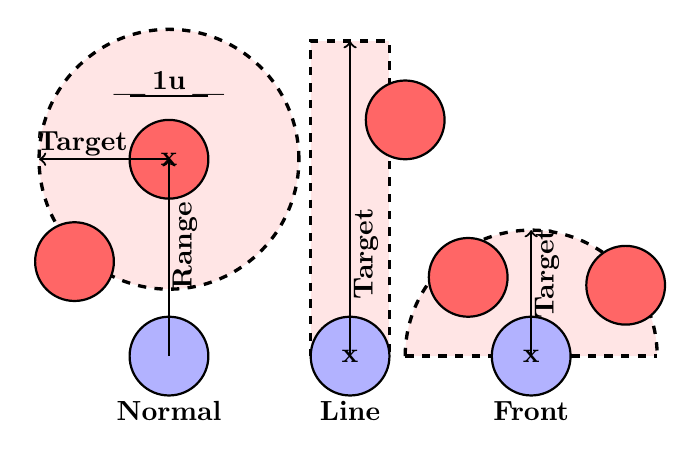
\begin{tikzpicture}[]
		\tikzstyle{test}=[thick, draw, circle, align=center]					
		%Normal
		\node[fill=blue!30!white, test,minimum size = 1cm](caster)at (0,0) {};
		\node[](t2)at (0,-0.7) {\bf Normal};
		\node[fill=red!10!white, test, very thick, dashed ,minimum size = 3.3cm](tarea)at (0,2.5) {};
		\node[fill=red!60!white, test,minimum size = 1cm](target)at (0,2.5) {};
		\node[fill=red!60!white, test,minimum size = 1cm](target)at (-1.2,1.2) {};
		\draw[thick, ->](0,0) -- node[] {}(0,2.5);
		\draw[thick, ->](0,2.5) -- node[] {}(-1.65,2.5);
		\node[rotate=90](t1)at (0.2,1.4) {\bf Range};
		\node[](t2)at (-1.1,2.7) {\bf Target};
		\node[](t3)at (0,2.5) {\bf x};
		\node[](fi)at (-0.5,3.3) {\bf |};
		\node[](se)at (0.5,3.3) {\bf |};
		\draw[thick, -](0.5,3.3) -- node[] {}(-0.5,3.3);
		\node[](sca)at (0,3.5) {\bf 1u};		
		%Line
		\node[draw, fill=red!10!white, rectangle, very thick, dashed ,minimum height = 4cm, minimum width=1cm](tarea)at (2.3,2) {};
		\node[fill=blue!30!white, test,minimum size = 1cm](caster)at (2.3,0) {};
		\node[](t2)at (2.3,-0.7) {\bf Line};
		\node[fill=red!60!white, test,minimum size = 1cm](target)at (3,3) {};
		\draw[thick, ->](2.3,0) -- node[] {}(2.3,4);
		\node[rotate=90](t1)at (2.5,1.3) {\bf Target};
		\node[](t3)at (2.3,0) {\bf x};		
		%Front
		\draw[fill=red!10!white, test, very thick, dashed] (3,0) arc (180:0:1.6cm);
		\draw[dashed, very thick, -](3,0) -- node[] {}(6.2,0);
		\node[fill=blue!30!white, test,minimum size = 1cm](caster)at (4.6,0) {};
		\node[](t2)at (4.6,-0.7) {\bf Front};
		\draw[thick, ->](4.6,0) -- node[] {}(4.6,1.6);
		\node[rotate=90](t1)at (4.8,1.05) {\bf Target};
		\node[fill=red!60!white, test,minimum size = 1cm](target)at (3.8,1) {};
		\node[fill=red!60!white, test,minimum size = 1cm](target)at (5.8,0.9) {};
		\node[](t3)at (4.6,0) {\bf x};
		\end{tikzpicture}
\end{figure}
%
\noindent
The illustration above shows the use of a ranged effect in the normal case and with the two
special target shapes \textbf{Line} and \textbf{Front}.
In situations where you are not able to measure distances accurately, you can also use the following descriptors to give a rough estimate:
%
\pagebreak
%
\begin{description}[leftmargin=*]
	\item[\accf{Adjacent}:] approxmimate distance of 1u or less.
	\item[\accf{Close}:] approxmimate distance between 1u and 3u.
	\item[\accf{Near}:] approxmimate distance between 3u and 6u.
	\item[\accf{Far}:] approxmimate distance of 6u or more.
\end{description}
%
\vfill
\subsubsection*{\hypertarget{status}{Status Effects}}
Status Effects alter your the combat potency in a positive or negative way for a limited duration.
Combatants can suffer multiple different Status Effects at once, but applying the same one twice only refreshes its duration. 
They can also be \textbf{Immune} to certain statuses, meaning they have no effect. 
Below is a list of all Status Effects.
\begin{description}[leftmargin=*]
	
	\item[\large\color{accent} \raisebox{-.2\height}{\includegraphics[width=\baselineskip]{./art/icons/doom.png}} \textbf{KO}:] 
	You are unconscious and your turns are skipped.
	You suffer KO when your current HP drops to 0 and your HP cannot be increased until this status is removed.  
	Immunity against KO only makes you immune against effects that cause it when above 0 HP.
		
	\item[\large\color{accent} \raisebox{-.1\height}{\includegraphics[width=\baselineskip]{./art/icons/blind.png}} \textbf{Blind}:] 
	Whenever you \hyperlink{action}{Attack} an enemy, he has \hyperlink{check}{Advantage} on the evasion check.
	
	\item[\large\color{accent} \raisebox{-.1\height}{\includegraphics[width=\baselineskip]{./art/icons/blink.png}} \textbf{Blink}:] 	
	Whenever you are targeted by an \hyperlink{action}{Attack}, you have \hyperlink{check}{Advantage} on the evasion check.
	
	\item[\large\color{accent} \raisebox{-.1\height}{\includegraphics[width=\baselineskip]{./art/icons/debrave.png} 
		\includegraphics[width=\baselineskip]{./art/icons/deprotect.png} \includegraphics[width=\baselineskip]{./art/icons/defaith.png} 
		\includegraphics[width=\baselineskip]{./art/icons/deshell.png}} \textbf{DeATR}:] 
	The according attribute is reduced by 3 (minimum 0), e.g. DeMAG reduces MAG. 
	
	\item[\large\color{accent} \raisebox{-.1\height}{\includegraphics[width=\baselineskip]{./art/icons/bravery.png} 
		\includegraphics[width=\baselineskip]{./art/icons/protect.png} \includegraphics[width=\baselineskip]{./art/icons/faith.png} 
		\includegraphics[width=\baselineskip]{./art/icons/shell.png}} \textbf{EnATR}:] 
	The according attribute is increased by 3, e.g. EnMAG increases MAG. 

	\item[\large\color{accent} \raisebox{-.1\height}{\includegraphics[width=\baselineskip]{./art/icons/immobile.png}} \textbf{Immobile}:] You are unable to move.

	\item[\large\color{accent} \raisebox{-.1\height}{\includegraphics[width=\baselineskip]{./art/icons/poison.png}} \textbf{Poison}:] 
	You take damage equal to 10\% of your maximum HP at the end of each turn, but cannot fall below 1 HP due to this effect.
	
	\item[\large\color{accent} \raisebox{-.1\height}{\includegraphics[width=\baselineskip]{./art/icons/silence.png}} \textbf{Silence}:]
	You cannot begin casting \hyperlink{action}{Magic} or using \hyperlink{action}{Techs}, but you can still \hyperlink{action}{Attack}.
	
	\item[\large\color{accent} \raisebox{-.1\height}{\includegraphics[width=\baselineskip]{./art/icons/stop.png}} \textbf{Sleep}:] 
	Your turns are skipped, but you wake up immediately if you take any damage.
	
	\item[\large\color{accent} \raisebox{-.1\height}{\includegraphics[width=\baselineskip]{./art/icons/zombie.png}} \textbf{Zombie}:] 
	All healing effects are reversed for you.
	Healing reduces your HP and effects that normally remove KO, inflict it to you instead.	
\end{description} 
%
\vspace*{0.5cm}
%
\example{Status Effects}
{
Noctis and his party fight \hyperlink{malboro}{Malboro}. 
The monster surprises them and uses his Bad Breath ability to inflict multiple Status Effects.
Prompto suffers Sleep and \textcolor{red}{Poison}. 
He cannot move or take actions and before his turn is finished, he loses \textcolor{red}{3} HP, because his maximum HP is 
\textcolor{red}{3}7.
Noctis suffers Silence and \textcolor{Plum}{Blind}.
He cannot use abilities, so he tries to \hyperlink{action}{Attack} Malboro. 
The monster~(AGI:~\textcolor{ForestGreen}{2}) rolls [1,6,4] on the evasion check, barely passing the 
\mbox{DC 12-\textcolor{ForestGreen}{2}} due to \textcolor{Plum}{Advantage}.
}
%
\pagebreak









\ofsection{Jogadores}
%
\ofquote{"Eu sou O Basch fon Rosenburg!"\\}{Vaan}\\\\
%
\includegraphics[width=\columnwidth]{./art/images/ff10-2.jpg}
%
\vfill
%
Cada jogador cria um \accf{Personagem} que é um protagonista no mundo de jogo criado pelo MJ. 
Para criar um personagem de Nível 1, copie ou imprima a \accf{Ficha de Personagem} da próxima página. 
Ela permite a você acompanhar vários aspectos de seu personagem, há também um exemplo de ficha preenchida, como guia. 
Escolha o \accf{Nome} de seu personagem e faça uma descrição curta sobre ele. 
Resuma a \accf{História} dele e explique suas motivações para se juntar ao grupo, considerando que o mais provável é que essa seja a sua primeira aventura séria. 
Escolha então uma \accf{Profissão} como explicado abaixo. 
Por fim, a subseção de \accf{Equipamento} explica como você pode personalizar os equipamentos iniciais de seu personagem. 
A tabela à direita resume os benefícios fornecidos em Níveis subsequentes, todos explicados em detalhes dentro desta seção.
%
\vfill
%
A \accf{Profissão} de seu personagem determina a proficiência em combate dele, incluindo habilidades, atributos e especialidade com equipamentos. 
Todas as profissões são detalhadas nas suas descrições logo após as fichas de personagem. 
Imprima ou copie a descrição daquela escolhida por você para usar como uma segunda página de sua ficha de personagem.
Os atributos de seu personagem iniciam em 0 e aumentam ao progredir em uma profissão. 
A descrição de cada uma delas mostra os atributos e habilidades recebidos em cada Nível, assim como todos os tipos de equipamentos que o seu personagem usa. 
Quando o seu personagem alcança o Nível 3, você tem que decidir entre um ou dois \accf{Arquétipos}. 
Arquétipos representam diferentes especializações de uma profissão e fornecem habilidades e atributos adicionais.
%
\newpage
%
\ofboxwithtitle{Exemplo: Criação de Personagem}
{
	Nós criamos um personagem chamado Vaan, que tem 17 anos, um garoto humano, loiro e de aparência atlética. 
	Vaan é um órfão que se vira na cidade grande roubando e geralmente age como uma figura paterna para os outros órfãos. 
	Ele sonha em ter sua própria aeronave e um dia ser um pirata dos céus. 
	Nós escolhemos a profissão Ladrão e de sua tabela de atributos, nós determinamos o PV máximo~(20), PM máximo~(19) e AGI (4), todos os outros atributos começam em 0. 
	Nós também anotamos que ele aprende a técnica Roubar. 
	Por fim, de nossos 1500G iniciais, compramos uma faca de Mithril, um Colete de Mithril, uma Pena de Fênix e 2 poções, o que nos deixa com 300G sobrando.
}
%
\vfill
%
\oftable{p{0.25\columnwidth} p{0.7\columnwidth}}
{\accf{Nível} & \accf{Benefício ganho}}
{
	1 & Profissão, Equipamento iniciante \ofrow
	2 & Talento \ofrow
	3 & Arquétipo \ofrow
	4 & Quebra de Limite, Equipamento avançado\ofrow
	5 & Esper \ofrow
	6 & Especialização \ofrow
	7 & Especialização \ofrow
	8 & Especialização, Equipamento Especialista \ofrow
	9 & Especialização \ofrow
	10 & Especialização
}
%
\vfill
%
Nos Níveis marcados como \accf{Especialização}, escolha um dos seguintes benefícios para seu personagem.\ofrow
\ofbullet{No início de cada uma das sessões, adicione um 6 extra à reserva de Dados de Fortuna.}
\ofbullet{Ganhe uma segunda escolha de Esper.}
\ofbullet{Ganhe uma segunda escolha de Talento.}
\ofbullet{Ganhe um segundo Modo Limite, permite a você obter Pontos Limite de 2 fontes. Além disso, o alcance máximo de sua Quebra de Limite é aumentado em 2.}
\ofbullet{Ganhe acesso ao segundo Arquétipo de sua profissão. Você pode alternar entre os dois sempre que for dormir e seus atributos e habilidades mudam de acordo com aquele ativo no momento.}
\ofbullet{Ao usar Magia, Técnica ou habilidade de Reação de seu Arquétipo, o custo de seu PM é reduzido pela metade e você ganha 1 Ponto Limite.}
\ofbullet{Armas e armaduras ganham um espaço de Matéria adicional enquanto estiverem equipadas.}
\ofbullet{Ganhe a capacidade de equipar uma arma ou armadura adicional à sua escolha.}
\ofbullet{Escolha um bônus da lista a seguir. Não é possível escolher o mesmo benefício mais de uma vez: PV+5, PM+5, FOR+1, DEF+1, MAG+1, RES+1.}
%
\clearpage
%
\ofcs{}
%
\ofcs{
	name=Lightning,
	%
	description={%
		\vspace*{-0.5cm}
		\begin{multicols}{2}
			Idade: 21\\Raça: humano\\Cabelo: rosa\\Altura: 1.70m\\Destra\\ Determinada\\ Fria
			\columnbreak\vspace*{-1.7cm}\\
			\hspace*{-1cm}\includegraphics[width=1\columnwidth]{./art/charactersheets/claire.jpg}
		\end{multicols}
		\vspace*{-0.9cm}
	},
	%
	story={\\
		Meus pais morreram quando eu era jovem.
		Eu criei minha irmã, Serah, e me alistei no exército, no qual me tornei sargento.
		Mas agora Serah está em perigo, então eu tenho que deixar o exército e para encontrá-la. \\\\\\
		"Não é uma questão de ser capaz ou não.\\Há coisas na vida que você simplesmente faz."
	},
	% 
	hpcur=19, hpmax=91, mpcur=13, mpmax=85, agi=3, movement=4u, evasiondc=9, str=5, def=3, mag=7, res=2, 
	%
	level=8, job=Mago Vermelho, archetype=Devastador\phantom{1234567}, talent=Corporações Guardião,
	%
	abilities={Cura, Fogo, Nevasca, Raio, Cegueira,\\ Veneno, Esuna, AnuElemento},
	specials={Sobrepujar, Conjuração Rápida}, status={Cegueira (1r), AnDEF (2r)},
	%
	limitbreak=Raiara, limitmode=Bravura, limitpoints=\ofcslimitbarfilled, 
	limitdesc={Uma chuva de raios irrompe dos céus sobre um inimigo dentro de 5u e todos a 2u dele. Todos os alvos afetados sofrem 2d+8 de dano de raio.},
	%
	summon=Odin, summonused=yes, summonsupport={Realize um pequeno ritual para invocar o cavalo de Odin, Sleipnir.\\}, summonability={Um alvo no campo de batalha é afetado por KO se falhar num teste de DF~8 ou recebe dano igual a 3x seu nível se passar.},
	%
	weapon=Lâmina Pistola Dobrável, weaponbox=\ofcsweaponboxexpert, weaponeffect=Ataque à distância após a habilidade, weapontype= contra-ataque de 11 a 12 no teste de evasão, armor=Uniforme da Corporação Guardiã, armorbox=\ofcsarmorboxbeginner, armortype=DEF~+1, accessory1=Bracelete do Poder, accessory1effect=FOR~+1,
	%
	gil=2009, inventory={\\Faca de sobrevivência, 5x Granada, 5x Poção maior,\newline3x Remédio, 2x Pena da Fênix, 1x Elixir}
}
%
\clearpage
\section*{\hypertarget{job}{Oficios}}
\addcontentsline{toc}{subsection}{Oficios}
%
"Fuera de mi silla, bufón. El rey se sienta ahí". \\
\indent -- Noctis 
%
\begin{center}
\includegraphics[width=\columnwidth]{./art/images/ff10-2.png} 
\end{center}
%
El oficio de tu personaje determina sus pericias en combate, incluidas las habilidades, atributos y equipo que pueden utilizar. La maestría en batalla de un personaje aumenta cuando se especializa en un oficio al ganar experiencia y niveles. Todos los oficios disponibles se detallan en la \textbf{Descripción de oficio}, detallada justo después de esta página. Te recomendamos que imprimas o copies la descripción del oficio elegido para usarla como segunda página de tu hoja de personaje. Los atributos de tu personaje empiezan en 0 y aumentan al mejorar en un oficio. La tabla de \textbf{Atributos básicos }muestra los aumentos de los atributos de tu personaje y el equipo que puede utilizar en el Nivel 1. La tabla de \textbf{Habilidades} muestra qué hechizos y técnicas aprenderá tu personaje en los diferentes niveles.

\subsubsection*{Arquetipo}
Cuando tu personaje llegue al \textbf{Nivel 4} en su oficio, debe decidir entre uno de sus dos arquetipos. Los arquetipos representan estilos de juego dentro de un oficio y se pueden considerar como diferentes enfoques para cumplir el mismo rol. Enfatizan el progreso en diferentes aspectos del combate, apoyando las habilidades de un personaje a través de beneficios pasivos. En el Nivel 4, el tipo de arquetipo elegido otorga a tu personaje habilidades \hyperlink{sabilities}{Pasivas y Reactivas}, así como también determina la progresión de atributos en los siguientes niveles.
%
\pagebreak
%
\subsubsection*{Superación de Límites}
A partir del \textbf{Nivel 5}, puedes elegir cualquiera de las habilidades de tu personaje para que sea su habilidad de Superación de Límites, que es una versión mejorada de la habilidad original. Solo puedes cambiar tu habilidad de Superación de Límites cuando subes de nivel. También puedes seguir utilizando la habilidad elegida en su versión original. Cuando utilizas la Superación de Límites, cuesta el doble de PM que de costumbre y obtiene \textbf{uno de los siguientes} efectos adicionales que elijas:
\begin{itemize}[leftmargin=*]  
	\item La cantidad de daño provocada o PV restaurados por la habilidad original se duplicará.
	\item Si la habilidad original afecta a un objetivo único, puedes dirigirlo a dos objetivos dentro de su alcance. Si la habilidad afecta a un área, la distancia máxima de la habilidad se duplicará.
	\item Si la habilidad original tiene un efecto que dura por un tiempo determinado, el mismo se duplicará. 
	\item Si la habilidad original requiere que tú o el objetivo pasen una tirada, puedes aumentar o disminuir la DC en 2 dependiendo de lo que te beneficie. 
\end{itemize}


\subsubsection*{Cambio de Oficio}
Puedes cambiar el oficio de tu personaje solo una vez durante la aventura después de subir de nivel. En lugar de aumentar el nivel de tu oficio inicial, tu personaje comienza en el nivel 1 del nuevo oficio. Al cambiar el oficio de tu personaje, mantienes todas las habilidades aprendidas, mejoras de atributos y competencia con el equipo de tu oficio inicial. La única excepción a esto es el atributo AGI, donde tu personaje solo obtiene la bonificación más alta entre los dos oficios. Sin embargo, tu personaje solo puede tener un máximo de 10 niveles en total entre ambos oficios. En consecuencia, la flexibilidad de cambiar de oficio es a costa de no ser capaz de convertirse en experto en ninguno.
\vspace{1cm}
%
\example{Cambio de Oficio}{
Después de luchar en el Santuario del Viento y de llegar a la cima, Bartz y su grupo se dan cuenta de que el Cristal del Viento ya ha sido destruido. De todas formas, el DJ otorga al grupo una subida de nivel y todos los miembros del grupo excepto Bartz pasan del nivel 2 al 3. Bartz recoge uno de los fragmentos del cristal y repentinamente siente un torrente de energía que le otorga poderes mágicos. En lugar de subir de nivel, cambia su oficio por el de Mago Negro, empezando en el nivel 1. Sin embargo, mantiene sus atributos y la capacidad de equipar espadas y armaduras de su antiguo oficio de Guerrero. Además, sus atributos se incrementan como se indica en la descripción del oficio de Mago Negro Nivel 1. La única excepción es el atributo AGI, que conserva la de su antiguo oficio ya que es más alto. Bartz también aprende los hechizos "Piro", "Hielo" y "Electro" además de las técnicas "Carga" y "Golpe fuerte" que ya sabe.
}
%
\clearpage
%
\ofjob{Dragoon}
{
	\ofquote{"Confident bastard, aren't you?"\\}{Kain}\\\\
	\includegraphics[width=\columnwidth]{./art/jobs/dragoon.jpg}\ofrow
	\accf{Dragoons} are masters of aerial combat, who strike their enemies with devastating attacks from the sky.
	They prefer spears as their weapon and have an affinity for the fire element. 
	Even though they are humanoid, it is said that Dragoons have the soul of a dragon.
}
{Spear}{Heavy Armor}{
	Level 1: & HP +23 & MP~+16 & AGI~+2,& STR~+1 \\
	Level 2: & HP~+10  & MP~+5 & STR~+1 & RES~+1 \\
	Level 3: & \multicolumn{3}{l}{Archetype Attribute Bonus} \\
	Level 4: & HP~+5  & MP~+10 & DEF~+2 &  	  \\
	Level 5: & HP~+10 & MP~+10 & STR~+1 & 		  \\ 
	Level 6: & HP~+10 & MP~+10 & RES~+1 		  \\
	Level 7: & HP~+10 & MP~+5  & STR~+1 & 	DEF~+1	  \\ 
	Level 8: & HP~+10 & MP~+10 & RES~+1 & 	 	  \\ 
	Level 9: & HP~+10  & MP~+10 & STR~+1 \\ 
	Level 10:& HP~+10  & RES~+1 & DEF~+2 
}{
	\ofjobtech{Jump}{3}{1r}{Single}{3u}{When you begin using this Tech, you jump 3u up into the air. After the cast time is up, you leap onto the target and make an Attack on him.}{}{1}\ofabilitygap
	\ofjobtech{Lancet}{3}{0r}{Single}{5u}{You reduce the target's HP and MP by 1d and increase your HP and MP by the same amount.}{}{2}\ofabilitygap
	\ofjobtech{Double Jump}{8}{1r}{Single}{3u}{When you begin using this tech, you jump 3u up into the air. After the cast time is up, you leap onto the target and make an Attack on him. You can then leap to another location within 3u. If you land on another enemy you can make an Attack on him too.}{}{6}\ofabilitygap
	\ofjobtech{Roar}{7}{0r}{5u}{Self}{All enemies in the target area make a DC 9 check and suffer Immobile for 1 round upon failure.}{\immobile}{8}\ofabilitygap
	\ofjobtech{Highwind}{24}{1r}{Single}{Self}{For the next 3 rounds, you stay up to 3u in the air from where you can move your usual distance and perform one of the following 2 actions without additional MP cost or cast time on each turn:\\ 
		\acc{Lance Barrage:} make an Attack against a target within 10u. If you hit, you score a Critical Hit.\\
		\acc{Fire Blast:} choose a target within 10u. He and all enemies within 2u of him suffer 4d fire damage.
	}{\fire}{10}
}{
	\ofarchetypet{Dragon Knight}
	{HP~+8 & MP~+12 & STR~+1 & RES~+2}
	{\ofarchetypetecha{Fire Breath}{7}{0r}{3u (front)}{Self}{You deal 2d fire damage to everyone in the target area.}{\fire}}
	{\ofarchetypepassive{Flametongue}{You gain permanent Resilience against fire damage. Furthermore, whenever you deal physical damage to an enemy, you can choose to let the damage dealt be of magical and fire type instead.}}
	{\ofarchetypereaction{Dragonheart}{Whenever you deal or receive fire damage, you gain EnSTR until the end of your next turn.}}
	{\ofarchetypetechb{Dragon Dive}{16}{1r}{3u}{7u}{When you begin using this Tech, you jump 3u up into the air. After the cast time is up you leap onto the target and deal 4d fire damage to everyone in the target area except yourself. Also, you create Hot Field in the target area that lasts for 3 rounds but does not affect you.}{\fire}}
}{
	\ofarchetypet{Valkyrie}
	{HP~+13 & MP~+7 & STR~+2 & DEF~+1}
	{\ofarchetypetecha{Full Thrust}{6}{0r}{5u (line)}{Self}{You dash forward in an up to 5u long line. Make an Attack on everyone in the way by making one damage roll that is applied to all targets that fail to evade.}{}}
	{\ofarchetypepassive{Duelist}{As long as you are in combat within 3u of one enemy and there is noone else within 3u of you, the STR bonus added to your Attacks and Abilities is doubled.}}
	{\ofarchetypereaction{Arm's Length}{Whenever an enemy walks within 2u of you, he has to make a DC~7 check and upon failure he cannot move any further towards you on this turn.}}
	{\ofarchetypetechb{Revenge}{12}{0r}{Single}{Weapon}{Make an Attack on an enemy that has damaged you since your last turn. On hit, you inflict the damage that he dealt to you before instead of your usual damage.}{}}
}
\thispagestyle{empty}
\subsection*{\huge Guerrero}
\vspace{0.3cm}
"Me da igual…". \\
\indent -- Squall 
\vspace{0.3cm} \\
Los Guerreros son especialistas en combate cuerpo a cuerpo debido a su poderosa capacidad física tanto en ataque como en defensa. Son expertos en el uso de espadas y armaduras, lo que les permite ser aún más peligrosos y resistentes. En su búsqueda de oponentes más fuertes, los Guerreros más experimentados saben que siempre hay un pez más gordo.
\vfill
\battrt{ \textbf{Nivel 1:} & PV~+25 & PM~+12 & AGI~+3 & FUE~+1 \\
 \textbf{Nivel 2:} & PV~+10 & PM~+5 & FUE~+1 & DEF~+1 \\
 \textbf{Nivel 3:} & PV~+10 & PM~+10 & RES~+1 &        \\
}{Espada}{Armadura Liviana, Armadura Pesada}
\vfill
\atypet{Caballero Oscuro} { \textbf{Nivel 4:} & PV~+5 & PM~+10 & FUE~+1 & RES~+1 \\ 
 \textbf{Nivel 5:} & PV~+10 & PM~+5 & DEF~+2 & 		  \\ 
 \textbf{Nivel 6:} & PV~+5 & PM~+10 & FUE~+2 &		  \\ 
 \textbf{Nivel 7:} & PV~+10 & PM~+5 & FUE~+1 & RES~+1 \\ 
 \textbf{Nivel 8:} & PV~+5 & PM~+5 & DEF~+1 & RES~+2 \\ 
 \textbf{Nivel 9:} & PV~+10 & PM~+5 & FUE~+1 & DEF~+1 \\ 
 \textbf{Nivel 10:}& PV~+10 & PM~+10 & RES~+1 &		  \\ 
} {Sacrificio} { Cuando hagas un \hyperlink{action}{Ataque} con éxito sobre un enemigo, puedes infligir daño \hyperlink{action}{Oscuro} equivalente a la mitad del daño original a ti y a todos los enemigos que se encuentren a ~3u. } {Precio de Sangre} { Siempre que un enemigo o un aliado (dispuesto) que se encuentre a 5u consuma PM, puedes obligarlo a que consuma sus PV en lugar de sus PM si tiene los suficientes PV para hacerlo. Luego, la mitad de ese valor se recupera a tus PV. }
\vfill
\atypet{Luchador} { \textbf{Nivel 4:} & PV~+10 & PM~+5 & FUE~+2 &        \\ 
 \textbf{Nivel 5:} & PV~+5 & PM~+10 & FUE~+1 & DEF~+1 \\ 
 \textbf{Nivel 6:} & PV~+10 & PM~+5 & DEF~+1 & RES~+1 \\ 
 \textbf{Nivel 7:} & PV~+5 & PM~+5 & FUE~+2 &        \\ 
 \textbf{Nivel 8:} & PV~+10 & PM~+5 & RES~+2 &        \\ 
 \textbf{Nivel 9:} & PV~+5 & PM~+10 & FUE~+1 & DEF~+1 \\ 
 \textbf{Nivel 10:}& PV~+10 & PM~+5 & DEF~+2 &        \\ 
} {Adrenalina} { Siempre que reduzcas los PV de un enemigo a 0, obtienes inmediatamente un turno extra. } {Punto Ciego} { Siempre que un enemigo en un radio de 1u inflija daño a un aliado o reciba daño de un aliado, inmediatamente puedes hacer un \hyperlink{action}{Ataque} sobre él. }
\pagebreak \\
\noindent {\Large\color{accent}\bf \uline{Habilidades\phantom{y}\hfill}}\\\\
\techt{Carga}{3}{0t}{Único}{Arma}{ Realiza un \hyperlink{action}{Ataque} contra el objetivo. Si lo golpeas, lo haces retroceder 1u además del daño infligido. }{}{1} \techt{Golpe Fuerte}{5}{0t}{Único}{Arma}{ Realiza un \hyperlink{action}{Ataque} en el que el objetivo tiene \hyperlink{check}{Ventaja} en la tirada de evasión. Si lo golpeas, haces \hyperlink{action}{Daño Crítico}. }{}{2} \techt{Rompearmadura}{10}{0t}{Único}{Arma}{ Realiza un \hyperlink{action}{Ataque} contra el objetivo. Si lo golpeas, el objetivo sufre \hyperlink{status}{disDEF} y \hyperlink{status}{disRES} por 3 turnos además del daño infligido. }{\dedef \deres}{3} \techt{Rompehuesos}{8}{0t}{Único}{Arma}{ Realiza un \hyperlink{action}{Ataque} contra el objetivo. Si lo golpeas, el objetivo queda \hyperlink{status}{Inmóvil} por 1 turno además del daño infligido. }{\immobile}{5} \techt{Enfocar}{6}{1t}{Objetivo}{Tú}{ Por los próximos 3 turnos, cada vez que realices un \hyperlink{action}{Ataque} sobre un enemigo, este tiene desventaja en la tirada de evasión. }{}{6} \techt{Valentía}{10}{1t}{2u}{Tú}{ Tú y todos los aliados que se encuentren en el área de efecto reciben \hyperlink{status}{aumFUE} y \hyperlink{status}{aumMAG} por 3 turnos. }{\enstr \enmag}{7} \techt{Vendaval}{8}{1t}{5u (línea)}{Tú}{ Realiza un \hyperlink{action}{Ataque} contra todos los que se encuentren en el área de efecto haciendo una sola tirada de daño que aplica a todos los afectados y que fallen la tirada de evasión. El daño infligido es de \hyperlink{type}{Viento}. }{\wind}{8} \techt{Andanada}{20}{1t}{5u}{Tú}{ Realiza un \hyperlink{action}{Ataque} contra todos los enemigos en el área de efecto haciendo una sola tirada de daño que aplica a todos los afectados y que fallen la tirada de evasión. Además, obtienes \hyperlink{status}{Reflejos} hasta el inicio de tu próximo turno. }{\blink}{9} \techt{Omnilátigo}{30}{0t}{Único}{Arma}{ Realiza 3 \hyperlink{action}{Ataques} separados contra el objetivo. Cada vez que el objetivo obtenga 4 o menos en la tirada de evasión, haces \hyperlink{action}{Daño Crítico}. }{}{10}
\pagebreak
\thispagestyle{empty}
\thispagestyle{empty}
\subsection*{\huge Summoner}
\vspace{0.3cm}
"I don’t like your plan. It sucks." \\
\indent -- Yuna 
\vspace{0.3cm} \\
Summoners are powerful spellcasters that can summon magical beasts to aid them in combat. 
They create a strong bond to their summon allowing the summoner to control their incredible powers to his
will. 
While the summoners themselves focus on using defensive magic, their summons can wreak havoc unlike any human being.
\vfill
\battrt{
	\textbf{Level 1:} & HP +16 & MP~+19 & AGI~+2 & MAG~+1 \\ 
	\textbf{Level 2:} & HP~+5  & MP~+10 & RES~+1 & STR~+1 \\ 
	\textbf{Level 3:} & HP~+10 & MP~+10 & MAG~+1 &         
}{Staff}{Robe}
\vfill
\atypet{Devout}
{	
	\textbf{Level 4:} & HP~+5  & MP~+10 & RES~+1 & DEF~+1 \\  
	\textbf{Level 5:} & HP~+10 & MP~+10 & MAG~+1 &        \\  
	\textbf{Level 6:} & HP~+5  & MP~+10 & MAG~+1 & RES~+1 \\  
	\textbf{Level 7:} & HP~+5  & MP~+10 & RES~+2 &        \\  
	\textbf{Level 8:} & HP~+10 & MP~+10 & DEF~+1 &		  \\  
	\textbf{Level 9:} & HP~+5  & MP~+10 & MAG~+1 & RES~+1 \\  
	\textbf{Level 10:}& HP~+10 & MP~+10 & MAG~+1 &        \\  
}
{Soulbind}
{	
	On your turn, your currently active summon can cast a spell where he can spend your MP in addition to his own and the spell's cast time is reduced by 1 round.
	You have to skip your own turn to use this effect.
}
{Sacrifice}
{	
	Whenever your currently active summon would receive any damage, you can choose to reduce your own HP by the same amount instead.
}
\vfill
\atypet{Evoker}
{		
	\textbf{Level 4:} & HP~+10 & MP~+5  & MAG~+1 & DEF~+1 \\  
	\textbf{Level 5:} & HP~+10 & MP~+10 & RES~+1 &		  \\  
	\textbf{Level 6:} & HP~+5  & MP~+10 & MAG~+1 & RES~+1 \\  
	\textbf{Level 7:} & HP~+10 & MP~+5  & DEF~+1 & RES~+1 \\  
	\textbf{Level 8:} & HP~+5  & MP~+10 & MAG~+2 &	      \\  
	\textbf{Level 9:} & HP~+5  & MP~+10 & RES~+1 & MAG~+1 \\  
	\textbf{Level 10:}& HP~+10 & MP~+10 & RES~+1 &		  \\  
}
{Channel}
{	
	On your turn, you can choose to cast a spell known by your currently active summon and the spell's cast time is reduced by 1 round. 
	The summon has to skip his turn to you use this effect.
}
{Lifesiphon}
{	
	Whenever you would receive any damage, you can choose to reduce the HP of your currently active summon by the same amount instead.
}
\pagebreak \\
\noindent {\Large\color{accent}\bf \uline{Abilities\phantom{y}\hfill}}\\\\
\spellt{Summon}{8}{3r}{Single}{Self}
{
	You summon a creature that acts with you on your turn, following your command.
	The summon is dismissed when you or the summon suffers \hyperlink{status}{KO}, but you can also dismiss it whenever you want.
	Once dismissed, you cannot summon the same creature again on the same day.
	All creatures that you can summon at different Levels are shown on the next page.
}{}{1}
\spellt{Pray}{5}{1r}{1u}{Self}{
	Everyone in the target area regains 1d HP. 
}{}{2}
\spellt{Image}{10}{1r}{1u}{3u}{
	The target gains \hyperlink{status}{Blink} for 3 rounds.
}{\blink}{4}
\spellt{Toad}{16}{1r}{Single}{3u}{
	The target makes a DC 8 check and is turned into a toad upon failure for 3 rounds or until he receives any damage.
	While being a toad, the target cannot talk or take any action and can only move 1u per turn.
}{}{6}
\spellt{Dispel}{20}{1r}{Single}{3u}{
	All \hyperlink{type}{Resiliences} and \hyperlink{status}{Immunities} of the target are removed for 3 rounds.
	Also, all beneficial \hyperlink{status}{Status Effects} that are active on the target when this spell takes effect are completely removed as well.
}{}{8}
\spellt{Twin Summon}{28}{5r}{Single}{Self}{
	You summon two different creatures that both follow your command and act with you on your turn.
	The summons are dismissed when you or they suffer \hyperlink{status}{KO}, but you can also dismiss them whenever you want.
	Once dismissed, you cannot summon the same creature again on the same day.
	All creatures that you can summon at different Levels are shown on the next page. 
}{}{10}
\vspace{5cm}
\pagebreak
\onecolumn
\noindent{\LARGE\color{accent}\bf \uline{Summons\hfill} \\} \\
\thispagestyle{empty}

\begin{multicols}{2}
\friendly{Carbuncle}{1}{\includegraphics[width=0.18\textwidth]{./art/monsters/carbuncle.png}}
{
	HP: & \hfill 20 & MP: & \hfill 36\\
	STR: & \hfill 1 & DEF: & \hfill 0 \\
	MAG: & \hfill 2 & RES: & \hfill 2 \\
	AGI: & \hfill 3 & Size: & \hfill S\\
}
{
	\textbf{Tackle}: 1d DMG\phantom{y} 
	
	\mspell{Reflect}{12}{1r}{Single}{3u}{The target gains a shield that reflects the next spell that targets them back to its caster.}{}		
}
\vspace{0.5cm} 
\friendly{Ifrit}{3}{\includegraphics[width=0.23\textwidth]{./art/monsters/ifrit.png}}
{
	HP: & \hfill 50 & MP: & \hfill 36\\
	STR: & \hfill 2 & DEF: & \hfill 3 \\
	MAG: & \hfill 1 & RES: & \hfill 0 \\
	AGI: & \hfill 3 & Size: & \hfill M\\
}
{
	\textbf{Claw}: 2d DMG \\
	\textbf{Resilience}:\fire \hfill \textbf{Weakness:}\ice
	
	\mspell{Fire}{4}{1r}{Single}{3u}{You deal 2d \hyperlink{fire}{fire} damage to the target.}{\fire}	
	\mtech{Hellfire}{12}{1r}{2u}{Self}{You deal 4d \hyperlink{type}{fire} damage to everyone in the target area except yourself.}{\fire}	
}
\vspace{0.5cm} 
\friendly{Shiva}{5}{\includegraphics[width=0.18\textwidth]{./art/monsters/shiva.png}}
{
	HP: & \hfill 60 & MP: & \hfill 80\\
	STR: & \hfill 1 & DEF: & \hfill 1 \\
	MAG: & \hfill 5 & RES: & \hfill 4 \\
	AGI: & \hfill 3 & Size: & \hfill M\\
}
{
	\textbf{Icicle}: 2d DMG, 3u Range \\
	\textbf{Resilience}:\ice \hspace*{\fill} \textbf{Weakness:}\fire
	
	\mspell{Deprotect}{5}{1r}{Single}{3u}{The target suffers \hyperlink{status}{DeDEF} for 3 rounds.}{\dedef}
	\mspell{Deshell}{5}{1r}{Single}{3u}{The target suffers \hyperlink{status}{DeRES} for 3 rounds.}{\deres}
	\mtech{Ice Wall}{10}{1r}{3u (line)}{3u}{
	You create a 3u tall and wide wall of ice that blocks the path for 5 rounds.
	The wall breaks down after 3 rounds or upon suffering a total of 30 damage.
	}{}
	\mspell{Diamond Dust}{20}{1r}{3u (front)}{Self}{
	All enemies in the target area suffer 6d \hyperlink{type}{ice} damage and \hyperlink{status}{Immobile} for 1 round.	
	}{\ice\immobile}		
}
\friendly{Phoenix}{7}{\includegraphics[width=0.2\textwidth]{./art/monsters/phoenix.png}}
{
	HP: & \hfill 70 & MP: & \hfill 90\\
	STR: & \hfill 0 & DEF: & \hfill 2 \\
	MAG: & \hfill 6 & RES: & \hfill 8 \\
	AGI: & \hfill 2 & Size: & \hfill M\\
}
{
	\textbf{Beak}: 1d DMG  \\ 
	\textbf{Immune}: \hyperlink{status}{All Status Effects} \hfill \textbf{Resilience:}\fire\holy
	
	\mspell{Protect}{5}{1r}{Single}{3u}{The target gains \hyperlink{status}{EnDEF} for 3 rounds.}{\enndef}
	\mspell{Shell}{5}{1r}{Single}{3u}{The target gains \hyperlink{status}{EnRES} for 3 rounds.}{\enres}
	\mspell{Curaga}{18}{1r}{1u}{3u}{Everyone in the target area regains 6d HP.}{}
	\mspell{Full-Life}{28}{3r}{Single}{3u}{Remove \hyperlink{status}{KO} from the target and fully heal his HP.}{\ko}	
	
}
\vspace{0.5cm} 
\friendly{Bahamut}{9}{\includegraphics[width=0.23\textwidth]{./art/monsters/bahamut.png}}
{
	HP: & \hfill 100 & MP: & \hfill 140\\
	STR: & \hfill 8 & DEF: & \hfill 6 \\
	MAG: & \hfill 7 & RES: & \hfill 4 \\
	AGI: & \hfill 4 & Size: & \hfill L\\
}
{
	\textbf{Claw}: 3d DMG, 2u Range \\
	\textbf{Immune}: \hyperlink{status}{All Status Effects} \hfill \textbf{Resilience:}\dark 

	\mtech{Obliterating Breath}{20}{1r}{3u (front)}{3u}{
	Everyone in the target area makes a DC 8 check and suffers 4d damage as well as \hyperlink{status}{Poison} and \hyperlink{status}{Blind} for 3 rounds upon failure.
	}{\poison \blind}
	\mspell{Banish}{30}{1r}{Single}{3u}{
	The target makes a DC 8 check and upon failure he is banished into another dimension and thus removed from the battlefield for 3 rounds.
	}{}
	\mspell{Megaflare}{40}{3r}{Single}{8u}{
		You deal 10d+20 \hyperlink{type}{fire} damage to the target.
	}{\fire}
	\mreaction{Final Attack}{If you are about to fall to 0 HP you may use one of your abilities without cost or cast time before falling \hyperlink{status}{KO}.}	
}
\end{multicols}
\twocolumn
\ofjob{Thief}
{
	\ofquote{"I PREFER the term ”treasure hunter!"\\}{Locke}\\\\
	\includegraphics[width=\columnwidth]{./art/jobs/thief.jpg}\ofrow
	\accf{Thieves} are mobile melee fighters, who can quickly traverse the battlefield and are difficult
	to hit with physical attacks. 
	They excel at "borrowing" items and money from enemies and have a heightened sense for worthwhile business. 
%	One would be advised to be careful when dealing with a Thief, they always have one more trick up their
%	sleeve than you would expect.
}
{Dagger}{Light Armor}{
	Level 1: & HP +20 & MP~+19 & AGI~+4 \\
	Level 2: & HP~+5  & MP~+10  & STR~+1 & DEF~+1 \\
	Level 3: & \multicolumn{3}{l}{Archetype Attribute Bonus} \\
	Level 4: & HP~+10 & MP~+5  & STR~+1 & DEF~+1 \\
	Level 5: & HP~+10 & MP~+10 & STR~+1 &        \\ 
	Level 6: & HP~+5  & MP~+5  & DEF~+2 & RES~+1 \\ 
	Level 7: & HP~+10 & MP~+10 & STR~+1 &        \\ 
	Level 8: & HP~+10 & MP~+5  & RES~+2 &        \\ 
	Level 9: & HP~+5  & MP~+10 & STR~+2 &        \\ 
	Level 10:& HP~+10 & MP~+10  & DEF~+1 
}{
	\ofjobtech{Steal}{4}{0r}{Single}{Weapon}{Make a DC 7 check and "borrow" something from the target if you succeed. Roll 1d and the you get 2d times 10G on 1 or 2, a Potion on a 3, a Remedy on a 4, an Ether on a 5 and a Phoenix Down on a 6. The item may also be determined in any other way by the GM.}{}{1} \ofabilitygap
	\ofjobtech{Flee}{3}{1r}{3u}{Self}{You and all allies in the target area can move twice as fast when running away from enemies for 3 rounds.}{}{2} \ofabilitygap
	\ofjobtech{Poison Dart}{6}{0r}{Single}{4u}{The target makes a DC~7 check and suffers 1d damage and one of the following Status Effects of your choice for 3 rounds upon failure: Poison, Immobile, Sleep}{}{4}\ofabilitygap
	\ofjobtech{Vanish}{8}{0r}{Single}{Weapon}{You become invisible for up to  5 rounds or until you take an action. While invisible, you gain Blink and have Advantage on all stealing related checks. Also, if you hit an Attack while invisible, you always score a Critical Hit.}{\blink}{6} \ofabilitygap
	\ofjobtech{Mirror Image}{23}{1r}{Single}{1u}{You create an exact copy of yourself. The clone lasts for up to 3 rounds and acts with you on your turn, following your command. The clone can use the same abilities except this one. You cannot create a clone while a previous one is still active.}{}{10}
}{
	\ofarchetypet{Ninja}
	{HP~+14 & MP~+11 & STR~+2}
	{\ofarchetypetecha{Throw}{4}{0r}{Single}{5u}{You throw a piece of equipment from your inventory on the target and deal an amount of damage depending on its equipment rank. The damage dealt is 1d for Beginner, 2d for Advanced and 3d for Expert level equipment. You can collect all thrown objects at the end of the battle.}{}}
	{\ofarchetypepassive{First Strike}{When an ally chooses you to take the next turn, you can immediately take it instead of waiting for a turn of the opposing party.}}
	{\ofarchetypereaction{Counter Attack}{When an enemy hits you with an Attack, you can immediately make an Attack on him if he is within range.}}
	{\ofarchetypetechb{Assassinate}{14}{0r}{Single}{3u}{Move to the target and make an Attack on him. If you hit, he makes a DC~7 check and suffers KO upon failure.}{\ko}}
}{
	\ofarchetypet{Treasure Hunter}
	{HP~+10 & MP~+20 & DEF~+1 & RES~+1}
	{\ofarchetypetecha{Quick Pockets}{6}{0r}{Single}{Self}{Make an Attack after which you can immediately use an Item.}{}}
	{\ofarchetypepassive{Gilionaire}{Whenever you deal damage to an enemy, you also receive an amount of Gil equal to the damage dealt.}}
	{\ofarchetypereaction{Counter Steal}{Whenever you evade an Attack by an enemy, you can immediately use "Steal" on him without any cost.}}
	{\ofarchetypetechb{Gil Toss}{8}{0r}{Single}{5u}{Throw an amount of Gil on the target up to maximum of 100G. The target suffers 1d damage for every 20G thrown.}{}}
}
\ofjob{White Mage}
{
	\ofquote{"Hey, that’s Cloud’s line! ’It’s too dangerous, I can’t get you involved...' Blah blah blah."\\}{Aerith}\\\\
	\includegraphics[width=\columnwidth]{./art/jobs/whitemage.jpg}\ofrow
	\accf{White Mages} are experts of defensive magic and boast a variety of recovery and protective spells.
	While mediocre in physical combat, they also feature incredible resistance against magic. 
%	Where others will succumb to the God of Death, a skilled White Mage will face him and say: "Not today".	
}
{Staff}{Robe}{
	Level 1: & HP~+19 & MP~+25 & AGI~+2 & STR~+1 \\
	Level 2: & HP~+5  & MP~+10 & MAG~+1 & RES~+1 \\
	Level 3: & \multicolumn{3}{l}{Archetype Attribute Bonus} \\
	Level 4: & HP~+10 & MP~+5 & MAG~+1 & DEF~+1	  \\
	Level 5: & HP~+5  & MP~+10 & RES~+1 &	STR~+1  \\ 
	Level 6: & HP~+5  & MP~+5 & MAG~+2 &        \\ 
	Level 7: & HP~+10  & MP~+10 & RES~+1 & DEF~+1 \\ 
	Level 8: & HP~+5 & MP~+5  & MAG~+2 & DEF~+1 \\ 
	Level 9: & HP~+5  & MP~+10 & RES~+1 &	MAG~+1   \\ 
	Level 10:& HP~+10 & MP~+10 & RES~+1 &	        
}{	
	\ofjobspell{Cure}{4}{0r}{Single}{3u}{The target regains 2d HP.}{}{1}\ofabilitygap
	\ofjobspell{Drain}{6}{0r}{Single}{3u}{Deal 1d damage to the target and increase your own HP by the total amount of damage dealt.}{}{2}\ofabilitygap
	\ofjobspell{Esuna}{6}{0r}{Single}{5u}{You remove all negative Status Effects except KO from the target.}{}{4}\ofabilitygap
	\ofjobspell{Curaga}{14}{1r}{2u}{5u}{Everyone in the target area regains 6d HP.}{}{6}\ofabilitygap
	\ofjobspell{Clear}{6}{0r}{5u}{50u}{You remove one active Field Effect within range.}{}{6}\ofabilitygap
	\ofjobspell{Holy}{21}{2r}{Single}{12u}{You deal 6d+45 holy damage to the target.}{\holy}{8}\ofabilitygap
	\ofjobspell{Auto-Life}{28}{2r}{Single}{3u}{You summon a guardian angel that watches over the target. The next time he falls KO, he is instantly revived with 1 HP. This effect does not stack and if not activated, it expires when the target goes to sleep.}{\ko}{10}
}{
	\ofarchetypet{Sage}
	{HP~+11 & MP~+9 & MAG~+2 & STR~+1}
	{\ofarchetypespella{Sleep}{6}{0r}{Single}{5u}{The target makes a DC 8 check and suffers Sleep for 3 rounds upon failure.}{\sleep}
	\vspace*{0.1cm}\\ \ofarchetypespella{Silence}{6}{0r}{Single}{5u}{The target makes a DC 8 check and suffers Silence for 3 rounds upon failure.}{\silence}}
	{\ofarchetypepassive{Ancient Wisdom}{Whenever you inflict on or more Status Effects on a target, you can also inflict DeDEF or DeRES on him for 3 rounds.}}
	{\ofarchetypereaction{Absorb MP}{When you are the target of an enemy ability, increase your MP by half the amount that the caster spent on it.}}
	{\ofarchetypespellb{Curse}{14}{1r}{Single}{5u}{The target makes a DC~9 check and upon failure he suffers 4d damage as well as Poison and Zombie for 3 rounds.}{}}
}{
	\ofarchetypet{Medic}
	{HP~+7 & MP~+13 & RES~+2 & DEF~+1}
	{\ofarchetypespella{Protect}{4}{0r}{Single}{5u}{The target gains EnDEF for 3 rounds.}{\enndef} \vspace*{0.1cm}\\ \ofarchetypespella{Shell}{4}{0r}{Single}{5u}{The target gains EnRES for 3 rounds.}{\enres}}
	{\ofarchetypepassive{Doctor's Code}{Whenever you use Magic on an ally within 1u, you can also immediately use an Item on him in addition.}}
	{\ofarchetypereaction{No Collateral}{Whenever you would be affected by a spell or tech that you are not the primary target of, you can choose that you and all other secondary targets are unaffected.}}
	{\ofarchetypespellb{Full-Life}{22}{2r}{Single}{5u}{You remove the KO status from the target and fully restore his HP.}{\ko}}
}
\thispagestyle{empty}
\subsection*{\huge Black Mage}
\vspace{0.3cm}
"You sure are a keen observer of the obvious, kupo!" \\
\indent -- Montblanc 
\vspace{0.3cm} \\
Black magic is a pathway to many abilities some consider to be unnatural. 
Black Mages are fragile in physical combat, but can wipe out multiple enemies from great distances and inflict nasty status effects. 
They can thus assert great control over the battlefield and are difficult to ignore for enemies. \\
\vfill
\battrt
{
	\textbf{Level 1:} & HP~+17 & MP~+21 & AGI~+2 & MAG~+1  \\
	\textbf{Level 2:} & HP~+5  & MP~+10 & STR~+1 & RES~+1  \\
	\textbf{Level 3:} & HP~+10 & MP~+10 & MAG~+1 &         
}
{Staff}
{Robe}
\vfill
\atypet{Arcanist}
{
	\textbf{Level 4:} & HP~+5  & MP~+5  & MAG~+2 & DEF~+1 \\ 
	\textbf{Level 5:} & HP~+5  & MP~+10 & RES~+1 & MAG~+1 \\ 
	\textbf{Level 6:} & HP~+5  & MP~+10 & RES~+1 & DEF~+1 \\
	\textbf{Level 7:} & HP~+10 & MP~+10 & MAG~+1 &  	  \\
	\textbf{Level 8:} & HP~+5  & MP~+10 & MAG~+1 & DEF~+1 \\
	\textbf{Level 9:} & HP~+10 & MP~+5  & RES~+1 & MAG~+1 \\
	\textbf{Level 10:}& HP~+5  & MP~+10 & RES~+2 &		  
}
{Magic Boost}
{	
	Whenever you cast \hyperlink{action}{Magic} that targets a single entity, you can choose to also target everyone within 1u of him. The damage dealt to secondary targets is halved.
}
{Critical Vanish}
{	
	Whenever you have more than 1 HP and an \hyperlink{action}{Attack} would reduce you to 0 HP, you remain at 1 HP and gain \hyperlink{status}{Blink} for 3 rounds or until you take an action.
}
\vfill
\atypet{Scholar}
{	
	\textbf{Level 4:} & MP~+10 & RES~+1 & DEF~+1 & MAG~+1 \\
	\textbf{Level 5:} & HP~+10 & MP~+10 & MAG~+1 		  \\
	\textbf{Level 6:} & HP~+5  & MP~+10 & RES~+1 & MAG~+1 \\
	\textbf{Level 7:} & HP~+5  & MP~+10 & MAG~+2  		  \\
	\textbf{Level 8:} & HP~+5  & MP~+10 & RES~+1 & DEF~+1 \\
	\textbf{Level 9:} & HP~+5  & MP~+10 & RES~+1 & MAG~+1  \\
	\textbf{Level 10:}& HP~+10 & MP~+10 & MAG~+1		  \\
}
{Turbo MP}
{	
	Whenever you begin casting \hyperlink{action}{Magic}, you can choose to double its range by also doubling the MP cost.
}
{Return Magic}
{	
	Whenever you suffer damage caused by \hyperlink{action}{Magic}, you can cast the same spell back to its caster.
	In doing this, you have to respect the cast time and MP cost of the spell.
	If you are already casting another spell, you have to break its concentration to use this effect. 
}
\pagebreak \\
\noindent {\Large\color{accent}\bf \uline{Abilities\phantom{y}\hfill}}\\\\
\spellt{Fire}{4}{1r}{Single}{3u}
{
	You deal 2d \hyperlink{type}{fire} damage to the target.
}{\fire}{1}
\spellt{Blizzard}{4}{1r}{Single}{3u}
{
	You deal 2d \hyperlink{type}{ice} damage to the target.
}{\ice}{1}
\spellt{Thunder}{4}{1r}{Single}{3u}
{
	You deal 2d \hyperlink{type}{lightning} damage to the target.
}{\lightning}{1}
\spellt{Blind}{6}{1r}{Single}{3u}
{
	The target makes a DC 8 check and suffers \hyperlink{status}{Blind} for 3 rounds upon failure.
}{\blind}{2}
\spellt{Bio}{8}{1r}{Single}{3u}
{
	The target makes a DC 8 check and suffers 2d damage and \hyperlink{status}{Poison} for 3 rounds upon failure.
}{\poison}{3}
\spellt{Firaga}{12}{2r}{Single}{5u}
{
	You deal 6d \hyperlink{type}{fire} damage to the target. 
}{\fire}{5}
\spellt{Blizzaga}{12}{2r}{Single}{5u}
{
	You deal 6d \hyperlink{type}{ice} damage to the target. 
}{\ice}{5}
\spellt{Thundaga}{12}{2r}{Single}{5u}
{
	You deal 6d \hyperlink{type}{lightning} damage to the target. 
}{\lightning}{5}
\spellt{Rasp}{4}{1r}{Single}{5u}
{
	You reduce the target's MP by 4d.
}{}{6}
\spellt{Quake}{22}{2r}{3u}{8u}
{
	Deal 8d \hyperlink{type}{earth} damage to everyone in the target area. 
}{\earth}{7}
\spellt{Flare}{24}{3r}{Single}{5u}
{
	You deal 9d+15 \hyperlink{type}{fire} damage to the target. 
}{\fire}{8}
\spellt{Doom}{28}{1r}{Single}{5u}
{
	The target makes a DC 8 check and suffers \hyperlink{status}{KO} after 3 rounds upon failure.
}{\ko}{9}
\spellt{Ultima}{40}{3r}{3u}{5u}
{
	Deal 10d+20 \hyperlink{type}{dark} damage to all enemies in the target area. 
}{\dark}{10}
\pagebreak
\ofjob{Red Mage}
{
	\ofquote{"Oh, I’ll show you how lightning strikes."\\}{Lightning}\\\\
	\includegraphics[width=\columnwidth]{./art/jobs/redmage.jpg}\ofrow
	\accf{Red Mages} are very versatile and possess a wide variety of abilities, but can also hold their own in melee combat. 
	Although they excel in neither discipline, Red Mages are still a force to be reckoned with.
}
{Rod or Sword}{Light Armor or Robe}{
	Level 1: & HP~+20 & MP~+21 & AGI~+3 & STR +1 \\
	Level 2: & HP~+5  & MP~+10 & MAG~+1 & DEF~+1 \\
	Level 3: & \multicolumn{3}{l}{Archetype Attribute Bonus}   \\
	Level 4: & HP~+10 & MP~+5  & STR~+1 & RES~+1 \\   
	Level 5: & HP~+5  & MP~+10 & MAG~+2 & 		  \\ 
	Level 6: & HP~+5 & MP~+10  & STR~+1 &	MAG~+1 \\ 
	Level 7: & HP~+10  & MP~+10 & DEF~+1 \\ 
	Level 8: & HP~+10 & MP~+5  & STR~+1 & MAG~+1 \\ 
	Level 9: & HP~+5  & MP~+10 & RES~+2 \\ 
	Level 10: & HP~+10 & MP~+10 & STR~+1 		  
}{	
	\ofjobspell{Cure}{4}{0r}{Single}{3u}{The target regains 2d HP.}{}{1}\ofabilitygap
	\ofjobspell{Fire}{4}{0r}{Single}{3u}{You deal 2d fire damage to the target.}{\fire}{2}\ofabilitygap
	\ofjobspell{Blizzard}{4}{0r}{Single}{3u}{You deal 2d ice damage to the target.}{\ice}{2}\ofabilitygap
	\ofjobspell{Thunder}{4}{0r}{Single}{3u}{You deal 2d lightning damage to the target.}{\lightning}{2}\ofabilitygap
	\ofjobspell{Blind}{6}{0r}{Single}{5u}{The target makes a DC~8 check and suffers Blind for 3 rounds upon failure.}{\blind}{4}\ofabilitygap	
	\ofjobspell{Esuna}{6}{0r}{Single}{3u}{You remove all negative Status Effects except KO from the target.}{}{6}\ofabilitygap
	\ofjobspell{NulElement}{10}{0r}{Single}{5u}{Choose an element (e.g. fire). The target does not suffer any damage of the chosen element for 3 rounds.}{}{8}\ofabilitygap
	\ofjobspell{Dualcast}{4}{0r}{Single}{Self}{You begin casting and concentrating on two spells of your choice simultaneously, but need to spend the necessary MP for both.}{}{10}
}{
	\ofarchetypet{Ravager}
	{HP~+6 & MP~+14 & MAG~+2 & RES~+1}
	{\ofarchetypespella{Poison}{6}{0r}{Single}{5u}{The target makes a DC~8 check and suffers Poison for 3 rounds upon failure.}{\poison}}
	{\ofarchetypepassive{Stagger}{Whenever you inflict one or more Status Effects on an enemy, he additionally suffers an amount of magical damage equal to your MAG.}}
	{\ofarchetypereaction{Swiftcast}{When you suffer damage from an enemy, you can immediately use an ability on him if he is within range.}}
	{\ofarchetypespellb{Imperil}{8}{0r}{Single}{5u}{The target suffers DeDEF and DeRES for 3 rounds.}{\dedef \deres} \ofabilitygap \ofarchetypespellb{Wall}{8}{0r}{Single}{5u}{The target gains EnDEF and EnRES for 3 rounds.}{\enndef \enres}}
}{
	\ofarchetypet{Spellblade}
	{HP~+14 & MP~+6 & STR~+2 & DEF~+1}
	{\ofarchetypetecha{Elemental Strike}{4}{0r}{Single}{Weapon}{Choose an element (e.g. fire) and make an Attack. If you hit, the damage is of magical type with the chosen element and you also add your MAG to the damage dealt.}{}}
	{\ofarchetypepassive{Magic Weapon}{Whenever you cast Magic, you can choose to store the spell inside your weapon. In this case, the spell's MP cost is halved. All stored spells take effect together with your next successful Attack and you can chose targets within their range including yourself. You cannot store more than two spells at once inside your weapon.}}
	{\ofarchetypereaction{Mana Shield}{Whenever your HP is reduced, you can instead choose to reduce your MP by the same amount.}}
	{\ofarchetypetechb{Phantom Blade}{5}{0r}{Single}{5u}{Make an Attack on a target within range as if you were standing next to him. This Attack cannot be evaded.}{}}
}
\thispagestyle{empty}
\subsection*{\huge Mago del Tiempo}
\vspace{0.3cm}
"¡El tiempo de jugar se acabó!" \\
\indent -- Ultimecia 
\vspace{0.3cm} \\
Los Magos del Tiempo son maestros del tiempo y el espacio, que comprenden que la imaginación es más importante que el conocimiento. Pueden manipular el flujo del tiempo y doblar el tejido de la realidad a su ventaja. Aunque los Magos del Tiempo rara vez luchan solos, pueden influir en gran medida durante una batalla con sus increíbles habilidades. \\
\vfill
\battrt{ \textbf{Nivel 1:} & PV~+17 & PM~+25 & AGI~+2 & MAG~+1 \\
 \textbf{Nivel 2:} & PV~+5 & PM~+10 & RES~+1 & FUE~+1 \\
 \textbf{Nivel 3:} & PV~+10 & PM~+10 & DEF~+1 &        \\
}{Bastón}{Túnica}
\vfill
\atypet{Ilusionista} { \textbf{Nivel 4:} & PV~+5 & PM~+10 & MAG~+2 &        \\ 
 \textbf{Nivel 5:} & PV~+10 & PM~+10 & RES~+1 &		  \\ 
 \textbf{Nivel 6:} & PV~+5 & PM~+10 & DEF~+1 & RES~+1 \\ 
 \textbf{Nivel 7:} & PV~+5 & PM~+10 & MAG~+1 & RES~+1 \\ 
 \textbf{Nivel 8:} & PV~+5 & PM~+10 & DEF~+1 & MAG~+1 \\ 
 \textbf{Nivel 9:} & PV~+5 & PM~+10 & RES~+2 &        \\ 
 \textbf{Nivel 10:}& PV~+5 & PM~+10 & MAG~+2 &		  \\ 
} {Ímpetu} { Siempre que te muevas al menos 1u en dirección a tu objetivo antes de lanzar un hechizo, el alcance del mismo aumenta 1u. } {Teletransportación Evasiva} { Siempre que seas objetivo de un \hyperlink{action}{Ataque}, puedes evadirlo teletransportándote a una ubicación que elijas a 3u de distancia. Si lo haces, no podrás utilizar ninguna habilidad por 1 turno, incluyendo esta. Tampoco puedes utilizar esta habilidad mientras estés concentrándote. }
\vfill
\atypet{Oráculo} { \textbf{Nivel 4:} & PV~+10 & PM~+5 & RES~+1 & MAG~+1 \\ 
 \textbf{Nivel 5:} & PV~+5 & PM~+10 & MAG~+1 & RES~+1 \\ 
 \textbf{Nivel 6:} & PV~+5 & PM~+10 & DEF~+2 &		   \\ 
 \textbf{Nivel 7:} & PV~+10 & PM~+10 & RES~+1 & 	      \\ 
 \textbf{Nivel 8:} & PV~+5 & PM~+10 & MAG~+2 &        \\ 
 \textbf{Nivel 9:} & PV~+5 & PM~+10 & RES~+1 & MAG~+1 \\ 
 \textbf{Nivel 10:}& PV~+5 & PM~+10 & RES~+2 &        \\ 
} {Ver Más Allá} { Puedes detectar siempre la presencia de personajes hostiles o monstruos que se encuentren en un radio de 50u. } {Karma} { Siempre tienes un dado en reserva, siendo el primero un 6. Siempre que alguien dentro de 3u de ti (incluido tú mismo) haga una tirada, puedes alterar el resultado intercambiando uno de los dados por el que tienes en reserva, si quien hizo la tirada te permite hacerlo. }
\pagebreak \\
\noindent {\Large\color{accent}\bf \uline{Habilidades\phantom{y}\hfill}}\\\\
\spellt{Gravedad}{5}{1t}{Único}{3u}{ El objetivo recibe 1d de daño mágico y solo puede moverse la mitad de la distancia habitual en su próximo turno. }{}{1} \spellt{Freno}{10}{1t}{Único}{3u}{ Por los próximos 3 turnos, el objetivo puede moverse o realizar una acción en su turno, pero no ambas. Además, todos sus tiempos de lanzamiento aumentan 1 turno. }{}{2} \spellt{Prisa}{10}{1t}{Único}{3u}{ Por los próximos 3 turnos, el objetivo puede hacer un movimiento o acción adicional en su turno y todos sus tiempos de lanzamiento se reducen 1 turno. }{}{3} \spellt{Gravedad++}{16}{2t}{2u}{5u}{ Todos los que se encuentren en el área de efecto reciben 4d de daño mágico y solo pueden moverse la mitad de la distancia habitual en su próximo turno. }{}{5} \spellt{Extender}{9}{0t}{Único}{5u}{ Elige un objetivo que esté siendo beneficiado o perjudicado por un estado alterado por un tiempo limitado. La duración de ese efecto se extiende 2 turnos. }{}{6} \spellt{Teletransportación}{14}{1t}{1u}{10u}{ Te teletransportas a una ubicación que puedas ver y que se encuentre dentro de un radio de 10u de ti. }{}{6} \spellt{Acelerar}{20}{0t}{Único}{3u}{El objetivo obtiene un turno extra inmediatamente después del tuyo. Este efecto no altera el orden de los turnos. }{}{7} \spellt{Levitar}{12}{1t}{Único}{3u}{ El objetivo puede levitar hasta 3u del piso por 3 turnos. Se mantiene su distancia habitual de movimiento. No puede recibir daño de \hyperlink{type}{Tierra} mientras esté flotando. }{}{8} \spellt{Paro}{32}{1t}{100u}{Tú}{ Detienes el tiempo para todos los que se encuentren en el área de efecto excepto para ti por hasta 1 minuto (6 turnos). Una vez que realices un \hyperlink{action}{Ataque} o lances \hyperlink{action}{Magia}, el tiempo vuelve a su curso normal nuevamente. }{}{9} \spellt{Paradoja}{45}{0t}{100u}{Tú}{ Vuelves 10 segundos en el tiempo (1 turno) dentro del área de efecto. Todas las entidades afectadas vuelven al estado (PV, PM, estados alterados) y posición del turno anterior. Sin embargo, tus PM actuales no están sujetos al efecto de "Paradoja". Además, todos los objetivos afectados no tienen ningún recuerdo de los sucesos ocurridos en el turno anterior. }{}{10}
\pagebreak

\thispagestyle{empty}
\subsection*{\huge Monk}
\vspace{0.3cm}
"Now I know why I have these stupid muscles!" \\
\indent -- Sabin 
\vspace{0.3cm} \\
Monks are adept melee fighters that posses a deadly combination of strength and technique.
While they do not have expertise in using magic, Monks can produce similarly incredible effects by tapping into their inner life force. 
A skilled monk absorbs what is useful, discards what is useless and adds what is specifically his own.
\vfill
\battrt
{
	\textbf{Level 1:} & HP +22 & MP~+10  & AGI~+4 & \\
	\textbf{Level 2:} & HP~+10 & MP~+5  & STR~+2 & \\
	\textbf{Level 3:} & HP~+10 & MP~+10 & DEF~+1 & \\
}{Claw}{Light Armor}
\vfill
\atypet{Black Belt}
{		
	\textbf{Level 4:} & HP~+10 & MP~+5  & STR~+2 &        \\ 
	\textbf{Level 5:} & HP~+5  & MP~+10 & DEF~+1 & RES~+1 \\
	\textbf{Level 6:} & HP~+10 & MP~+5  & STR~+1 & RES~+1 \\
	\textbf{Level 7:} & HP~+10 & MP~+5  & STR~+1 & DEF~+1 \\ 
	\textbf{Level 8:} & HP~+10 & MP~+5  & STR~+2 &        \\
	\textbf{Level 9:} & HP~+5  & MP~+10 & STR~+1 & RES~+1 \\ 
	\textbf{Level 10:}& HP~+10 & MP~+10 & STR~+1 &        \\ 
}
{Unscarred}
{	
	As long as your current HP is equal to your maximum HP, the STR bonus that is added to the damage dealt by your \hyperlink{action}{Attacks} is doubled.
}
{Strikeback}
{	
		Whenever you successfully evade an \hyperlink{action}{Attack} by an enemy, immediately make an \hyperlink{action}{Attack} on him.
}
\vfill
\atypet{Templar}
{	
	\textbf{Level 4:} & HP~+5  & MP~+10 & STR~+1 & RES~+1 \\ 
	\textbf{Level 5:} & HP~+10 & MP~+5  & DEF~+2 & 		  \\ 
	\textbf{Level 6:} & HP~+5  & MP~+10 & STR~+2 & 		  \\ 
	\textbf{Level 7:} & HP~+10 & MP~+5  & RES~+2 & 	      \\ 
	\textbf{Level 8:} & HP~+10 & MP~+10 & STR~+1 & 	      \\ 
	\textbf{Level 9:} & HP~+5  & MP~+10 & RES~+1 & STR~+1 \\ 
	\textbf{Level 10:}& HP~+10 & MP~+10 & STR~+1 & 		  \\ 
}
{Lifestream}
{	
	If you do not have enough MP to use an ability you can instead choose to reduce your HP by the amount of its MP cost in order to use it.
}
{Replenish MP}
{	
	Whenever you suffer \hyperlink{type}{physical} damage, increase your MP by 1d.
}
\pagebreak \\
\noindent {\Large\color{accent}\bf \uline{Abilities\phantom{y}\hfill}}\\\\
\techt{Boost}{3}{0r}{Single}{Self}
{
	You gain \hyperlink{status}{EnSTR} until the end of your next turn. 
}{\enstr}{1}
\techt{Chakra}{6}{1r}{Single}{Self}
{
	You regain 1d HP and remove all \hyperlink{status}{Status Effects} that you are currently suffering.
}{}{2}
\techt{Kick}{8}{0r}{1u}{Self}
{
	You make an \hyperlink{action}{Attack} against all enemies within 1u of you, by making one damage roll that applies to all affected targets that fail to evade. All targets that fail to evade are also knocked back by 1u. 
}{}{3}
\techt{Pummel}{9}{0r}{Single}{Weapon}
{
	You make 2 consecutive \hyperlink{action}{Attacks} against the target. 
}{}{5}
\techt{Vigilance}{6}{0r}{Single}{Self}
{
	You gain \hyperlink{status}{Blink} until the end of your next turn. 
}{\blink}{6}
\techt{Revive}{16}{3r}{Single}{1u}
{
	You remove \hyperlink{status}{KO} from the target and increase his HP by~1. 
}{\ko}{6}
\techt{Aurablast}{7}{0r}{Single}{3u}
{
	You deal 4d \hyperlink{type}{magical} damage to the target.
}{}{7}
\techt{Meteor Strike}{16}{0r}{Single}{Weapon}
{
	You slam the target into the ground dealing 7d damage.
	In doing this, you can also leap to a location of your choice within 3u.
}{}{8}
\techt{Blitz}{5}{0r}{Single}{Self}
{
	You use two different \hyperlink{action}{Techs} consecutively in the same turn.
	In doing this, you have to respect additional MP costs and cast times of both \hyperlink{action}{Techs}.
	If an enemy is affected by both \hyperlink{action}{Techs}, deal an additional 4d damage to him.
}{}{9}
\techt{Final Heaven}{24}{0r}{Single}{Weapon}
{
	You deal 6d damage to the target and knock him back by 3u.
	If he hits a wall or a similarly solid object in doing so, you deal another 4d damage to him.
}{}{10}
\pagebreak
\thispagestyle{empty}
\subsection*{\huge Sentinela}
\vspace{0.3cm}
"Permítanme destruir sus delirios de grandeza" \\
\indent -- Beatrix 
\vspace{0.3cm} \\
Los Sentinelas son maestros del combate defensivo que raramente caerán en batalla. Sus habilidades especiales les permiten no solo soportar grandes cantidades de daño, sino que también proporcionan protección a sus aliados. Un Sentinela competente es el último bastión entre el grupo y una muerte certera.
\vfill
\battrt { \textbf{Nivel 1:} & PV~+28 & PM~+13 & AGI~+3 & DEF~+1 \\
\textbf{Nivel 2:} & PV~+10 & PM~+10 & FUE~+1 & RES~+1 \\
\textbf{Nivel 3:} & PV~+10 & PM~+10 & DEF~+1 &  
}{Espada}{Armadura Pesada}
\vfill
\atypet{Defensor} { \textbf{Nivel 4:} & PV~+10 & PM~+5 & DEF~+1 & FUE~+1 \\ 
 \textbf{Nivel 5:} & PV~+10 & PM~+5 & FUE~+1 & DEF~+1 \\ 
 \textbf{Nivel 6:} & PV~+10 & PM~+10 & RES~+1 &        \\ 
 \textbf{Nivel 7:} & PV~+10 & PM~+5 & FUE~+1 & DEF~+1 \\
 \textbf{Nivel 8:} & PV~+10 & PM~+5 & RES~+1 & DEF~+1 \\
 \textbf{Nivel 9:} & PV~+10 & PM~+5 & DEF~+2 & 		\\ 
 \textbf{Nivel 10:}& PV~+10 & PM~+5 & FUE~+2 &        \\
} {Provocar} { Siempre que \hyperlink{action}{Ataques} a un enemigo con éxito, puedes intentar provocarlo. Si lo haces, el objetivo debe hacer una tirada con DC~7. Si falla, debe dirigir una acción hacia ti en su siguiente turno, si es posible. } {Bloqueo} { Cuando un enemigo que se encuentre a 1u de ti intenta alejarse de tu posición, debe hacer una tirada con DC 7. Si falla, sufre \hyperlink{status}{Inmóvil} hasta el comienzo de su próximo turno, evitando que se mueva más en este turno. }
\vfill
\atypet{Paladín} { \textbf{Level 4:} & PV~+10 & PM~+10 & DEF~+1 \\
 \textbf{Nivel 5:} & PV~+10 & PM~+5 & RES~+1 & DEF~+1 \\ 
 \textbf{Nivel 6:} & PV~+10 & PM~+5 & FUE~+2 &        \\
 \textbf{Nivel 7:} & PV~+10 & PM~+5 & RES +2 &        \\
 \textbf{Nivel 8:} & PV~+10 & PM~+5 & FUE~+1 & DEF~+1 \\
 \textbf{Nivel 9:} & PV~+10 & PM~+10 & FUE~+1 &        \\
 \textbf{Nivel 10:}& PV~+5 & PM~+10 & RES~+1 & DEF +1 \\
} {Guardia Sagrada} { Siempre que haya un aliado a 1u de ti, ambos reciben \hyperlink{status}{Reflejos}. Este beneficio no puede aplicarse a más de un aliado al mismo tiempo. } {Cubrir} { Siempre que un aliado que se encuentre a 1u de ti reciba daño \hyperlink{type}{Físico}, puedes elegir recibir la mitad del daño total en vez de que tu aliado reciba todo el daño. }
\pagebreak \\
\noindent {\Large\color{accent}\bf \uline{Habilidades\phantom{y}\hfill}}\\\\
\techt{Guardia}{3}{0t}{Único}{Tú}{ Obtienes \hyperlink{status}{aumDEF} hasta el final de tu próximo turno. }{\enndef}{1} \techt{Primeros Auxilios}{5}{0t}{Único}{1u}{ Elige a un objetivo que haya recibido daño este turno o el anterior (incluido tú). El objetivo recupera 2d de PV. }{}{2} \techt{Rompebrazo}{10}{0t}{Único}{Arma}{ Realiza un \hyperlink{action}{Ataque} sobre el objetivo. Si lo golpeas, el objetivo sufre \hyperlink{status}{disFUE} y \hyperlink{status}{disMAG} por 3 turnos además del daño infligido. }{\destr \demag}{3} \techt{Guardia Vital}{9}{1t}{Único}{Tú}{ Obtienes \hyperlink{status}{aumDEF} por 3 turnos. Cuando el efecto termine, recuperas 2d de PV. }{\enndef}{5} \spellt{Muro de Tierra}{10}{1t}{3u (línea)}{3u}{ Creas un muro de 3u de alto y ancho que bloquea el paso. El muro se rompe después de 5 turnos o tras sufrir un total de 30 puntos de daño. }{}{6} \techt{Hostigar}{8}{1t}{Único}{3u}{ El objetivo hace una tirada con DC 8. Si falla, queda \hyperlink{status}{Inmóvil} por 3 turnos. }{\immobile}{7} \spellt{Astra}{11}{1t}{Único}{3u}{ Por los próximos 3 turnos, el objetivo es \hyperlink{status}{Inmune} a todos los \hyperlink{status}{Estados Alterados}. }{}{8} \techt{Segar}{16}{0t}{Único}{Arma}{ Realiza un \hyperlink{action}{Ataque} sobre el objetivo. Si lo golpeas, el objetivo recibe como daño la diferencia entre tus PV actuales y tus PV máximos en lugar del daño normal. }{}{9} \techt{Guardia Total}{30}{1t}{Único}{Tú}{ Por los próximos 3 turnos, no recibes ningún daño. }{}{10}
\pagebreak

\thispagestyle{empty}
\subsection*{\huge Marksman}
\vspace{0.3cm}
"I play the leading man; who else?" \\
\indent -- Balthier 
\vspace{0.3cm} \\
Marksmen are experts of all kinds of ranged weapons that strike from great distance. 
Skilled Marksmen can see through their enemies, allowing them to know target's strengths and weaknesses. 
Therefore they can not only deal significant ranged damage, but also disable enemies with special techniques. 
For the Marksman there is but one rule: hunt or be hunted.
\vfill
\battrt
{
	\textbf{Level 1:} & HP +19 & MP~+12 & AGI~+2 & STR +1 \\
	\textbf{Level 2:} & HP~+5  & MP~+10 & STR~+1 & DEF~+1 \\
	\textbf{Level 3:} & HP~+10 & MP~+5  & STR~+1 & RES~+1 \\
}{Bow, Gun}{Light Armor}
\vfill
\atypet{Ranger}
{	
	\textbf{Level 4:} & HP~+10 & MP~+10 & STR~+1 &        \\
	\textbf{Level 5:} & HP~+5  & MP~+10 & DEF~+2 &        \\
	\textbf{Level 6:} & HP~+10 & MP~+10 & RES~+1 &        \\
	\textbf{Level 7:} & HP~+5  & MP~+10 & STR~+1 & RES~+1 \\
	\textbf{Level 8:} & HP~+5  & MP~+5  & RES~+1 & DEF~+2 \\
	\textbf{Level 9:} & HP~+5  & MP~+10 & RES~+1 & STR~+1 \\
	\textbf{Level 10:}& HP~+10 & MP~+5  & STR~+2 &        \\
}
{Recoil}
{	
	Whenever you make a successful \hyperlink{action}{Attack}, you can immediately move 1u even when wielding a bow.
}
{Magic Evade}
{	
	You can evade \hyperlink{action}{Magic} by passing an evasion check, the same way you evade \hyperlink{action}{Attacks}.
}
\vfill
\atypet{Sniper}
{	
	\textbf{Level 4:} & HP~+5  & MP~+5  & STR~+2 & RES~+1 \\
	\textbf{Level 5:} & HP~+10 & MP~+10 & DEF~+1 &		  \\
	\textbf{Level 6:} & HP~+5  & MP~+10 & STR~+1 & DEF~+1 \\
	\textbf{Level 7:} & HP~+5  & MP~+5  & STR~+1 & RES~+2 \\
	\textbf{Level 8:} & HP~+5  & MP~+10 & DEF~+1 & RES~+1 \\
	\textbf{Level 9:} & HP~+10 & MP~+5  & STR~+2 &        \\
	\textbf{Level 10:}& HP~+5  & MP~+5  & RES~+1 & STR~+2 \\
}
{Concentrate}
{	
	Whenever you \hyperlink{action}{Attack} an enemy, he has \hyperlink{check}{Disadvantage} on the evasion check.
}
{Auto-Item}
{	
	Whenever you suffer any damage, you can immediately use an \hyperlink{item}{Item}.
	You can only use this effect once per round.
}
\pagebreak \\
\noindent {\Large\color{accent}\bf \uline{Abilities\phantom{y}\hfill}}\\\\
	\techt{Big Shot}{3}{0r}{Single}{Weapon}
	{
		Make an \hyperlink{action}{Attack} on the target. 
		If you hit, the damage dealt ignores the target's DEF.
	}{}{1}
	\techt{Lay Trap}{4}{1r}{1u}{Self}{
		You set a trap where you are standing.
		An enemy that walks over it makes a DC 9 check and suffers 2d damage and \hyperlink{status}{Immobile} for 1 round upon failure.
		The trap disappears once it is activated.
	}{\immobile}{2}
	\spellt{Libra}{5}{0r}{Single}{3u}
	{
		You analyse the target thoroughly and know his \hyperlink{type}{Resiliences}, \hyperlink{type}{Weaknesses}, \hyperlink{type}{Immunities}, as well as his current HP and MP.
	}{}{3}
	\techt{Quick Shot}{9}{0r}{Single}{Weapon}
	{
		You make an \hyperlink{action}{Attack} after which you can immediately begin using an \hyperlink{action}{Ability} or \hyperlink{item}{Item} on the same turn.
	}{}{5}
	\techt{Pierceshot}{7}{0r}{10u (line)}{Self}
	{
		You make an \hyperlink{action}{Attack} against all targets in a line, by making one damage roll that applies to everyone that fails to evade.	
	}{}{6}
	\techt{Poison Ammo}{8}{0r}{Single}{Weapon}
	{
		Make an \hyperlink{action}{Attack} on the target. 
		If you hit, the damage dealt is \hyperlink{type}{magical} and the target makes a DC 8 check. 
		Upon failure, he suffers \hyperlink{status}{Poison} for 3 rounds.	
	}{\poison}{7}
	\techt{Target MP}{4}{1r}{Single}{Weapon}
	{
		Make an \hyperlink{action}{Attack} on the target.
		If you hit, you reduce his MP by the amount of damage dealt instead of his HP.
	}{}{8}
	\techt{Smoke Bomb}{12}{1r}{3u}{5u}
	{
		You create a smoke cloud that inhibits vision in the target area for 5 rounds.
		Everyone inside the cloud suffers \hyperlink{status}{Blind}, but gains \hyperlink{status}{Blink}.
	}{\blind\blink}{9}
	\techt{Barrage}{22}{1r}{Single}{Self}
	{
		For up to 3 rounds you make 2 consecutive \hyperlink{action}{Attacks} as your action on every turn.
		As long as this effect is active, you cannot move or take other actions.
		You can choose to end this effect at the start of every turn.
	}{}{10}
\pagebreak



\ofsubsection{Equipamento}
%
\ofquote{"Ah, é mesmo, você não sabia? Hoje em dia, tudo que se precisa para realizar seus sonhos é dinheiro e poder."\\}{President Shinra}\\
%
\includegraphics[width=\columnwidth]{./art/images/ff1.jpg}
%
\vfill
%
A força de combate de um personagem pode ser melhorada através de seu \accf{Equipamento}.
Enquanto \accf{Armas} aumentam o dano causado, \accf{Armaduras} protegem contra possíveis danos e \accf{Acessórios} servem de complemento.
Cada equipamento fornece um efeito \accf{Único} e, armas e armaduras têm um \accf{Tipo} adicional de efeito específico ao seu tipo.
Armas têm alcance de 1u, exceto se especificado o contrário.
Ao invés de armaduras, os personagens também podem usar roupas comuns que fornecem DEF~1.
Acessórios podem ser usados por todos, mas os personagens só podem equipar armas e armaduras determinadas pela sua profissão.
Embora, os personagens possam usar \accf{Itens}, que forneçam benefícios rápidos dentro e fora do combate, eles são consumidos após seu uso. 
Equipamentos são categorizados em diferentes \accf{Níveis de Equipamento} a depender de sua potência e raridade.
Enquanto todos carregarem equipamento Iniciante, é necessário alcançar Níveis mais altos para usar equipamentos Avançados e Especialistas.
Os detalhes de cada Nível de Equipamento está disponível na tabela abaixo.
%
\vfill
%
\oftable{p{0.2\columnwidth} p{0.125\columnwidth} p{0.15\columnwidth} p{0.15\columnwidth} p{0.3\columnwidth}}
{\accf{Nível de\newline Equip.} & \accf{Nível} & \accf{Dano da Arma} & \accf{Armadura\newline DEF/RES} & \accf{Valor\newline Aprox.}}
{
	Iniciante & 	1 - 3 	& 1d & +0 / +0   & 500G\ofrow
	Avançado &  4 - 7   & 2d & +1 / +1   & 2000G\ofrow
	Especialista   &  8 - 10	& 3d & +2 / +2   & 4000G 
}
%
\vfill
%
Todos os itens e posses não equipados são armazenados no \accf{Inventário} do personagem.
Eles podem ser saqueados de adversários derrotados ou recebidos como recompensas ao se completar missões.
Mas o grupo também pode comprar ou vender produtos específicos em lojas ou mercadores.
A moeda usada para comércio é chamada de \accf{Gil} (\accf{G}) e normalmente vem em forma de moedas de ouro.
Você pode tentar comprar e vender quase qualquer coisa, enquanto houver alguém disposto a negociar.
%
\newpage
%
\ofboxwithtitle{Exemplo: Comércio}
{
	Terra e seu grupo visitam uma casa de leilão para conseguir itens raros. 
	Hoje é o dia de sorte deles, o item em leilão é uma Chocobo falante!
	O grupo está impressionado com a talentosa criatura e decide usar todas as suas economias, um total de 10.000G!
	Parece que o lance deles está superando ao de todos, mas no último segundo, um pai amável anuncia 500.000G e adquire a Chocobo como um presente para seu filho.
	Talvez o grupo tenha mais sorte (ou dinheiro) da próxima vez...
}
%
\vfill
%
\ofquote{"Cloud, assine isso. É um contrato que diz que quando a guerra acabar, todas as matérias pertencerão a mim."}{Yuffie}
%
\vfill
%
Armas e armaduras podem ser melhoradas através do uso de \accf{Matéria}.
Matéria normalmente parece com um cristal, que concentra forças mágicas e pode ser usada por qualquer um.
Elas podem ser encaixadas em espaços nas armas ou armaduras e garantir ao usuário efeitos adicionais.
Aquelas encaixadas também podem ser removidas, trocadas ou armazenadas com facilidade.
A menos que especificado o contrário, cada arma e armadura pode carregar uma matéria, enquanto roupas e acessórios nenhuma.
Matérias podem ser divididas em duas categorias: Comando e Suporte.
Matérias de Comando permitem ao usuário usar novas habilidades, enquanto as de Suporte garantem efeitos passivos.
Se uma Matéria permite o uso de uma habilidade existente, o usuário deve atender às essas exigências, como custo em PM e tempo de conjuração.
%
\vfill
%
\ofquote{"Sim, as doze armas lendárias. São armas. São lendárias. Há até doze delas."\\}{Ghido}
%
\vfill
%
A menos que o MJ diga o contrário, cada personagem tem 1.500G no Nível~1, com esse valor ele pode comprar seus equipamentos iniciais, desta forma:
\ofrow
\ofbullet{Comprar qualquer arma Iniciante por 500G ou uma arma Mithril por 250G.}
\ofbullet{Comprar uma armadura Iniciante por 500G, uma armadura Mithril por 250G ou roupas por 100G.}
\ofbullet{Opcional, comprar qualquer conjunto de itens que puder pagar.}
\ofbullet{Opcional, compre um acessório Iniciante por 500G.}
\ofbullet{Opcional, compre uma Matéria que possa pagar.}\vspace*{-0.25cm}\\
As próximas páginas possuem vários exemplos de equipamentos para se escolher.
As tabelas detalham efeitos únicos de cada um, assim como os tipos diferentes de armas e armaduras.
Todas as armas e armaduras listadas são do nível Iniciante, exceto se o MJ dizer o contrário.
Note que a ficha de personagem fornece vários campos para acompanhar o inventário assim como os equipamentos atuais e seus efeitos.
%
\clearpage
%
\newcommand{\ofequipnote}[1]{\multicolumn{2}{p{\columnwidth}}{\hspace*{-0.15cm}\parbox{0.97\columnwidth}{\accf{Efeito Tipo:} #1}}}
\oftable{p{0.22\columnwidth} p{0.7\columnwidth}}
{\oficonweapon\accf{Arcos} & \accf{Efeito Único}}
{
	Arco Mythril & Possui um espaço de Matéria extra. \ofrow
	Arco Élfico & Adicione 3 ao dano ao atingir um alvo que tenha algum Efeito de Estado.\ofrow
	Arco\newline Assassino & Num Acerto Crítico, o alvo sofre KO. \ofrow
	Besta & Não sofre da penalidade do seu tipo de efeito, mas só tem alcance de 3u. \ofrow
	Aplu & Ignora efeitos que permitem ao alvo ter Vantagem no teste de evasão, exceto seu próprio tipo de efeito. \ofrow
	Anteros & Quando o alvo rolar 5 ou menos no teste de evasão, ele fica Cego por 3 rodadas.\ofrow
	\ofequipnote{Arcos tem alcance de 5u. Se você atacar ou usar uma técnica que precise atacar e se mover no mesmo turno, o alvo tem vantagem no teste de evasão.\phantom{y}}
}
%
\vfill
%
\oftable{p{0.22\columnwidth} p{0.7\columnwidth}}
{\oficonweapon\accf{Arma\newline de Fogo} & \accf{Efeito Único}}
{
	Arma Mythril & Possui um espaço de Matéria extra. \ofrow
	Fomalhaut & O dano causado é do tipo mágico. \ofrow
	Abelhinha & Num Acerto Crítico, aja novamente. \ofrow
	Metralhadora & Se o alvo se evadir do seu ataque, ele ainda sofre metade do dano. \ofrow
	Baforada de\newline Dragão & O dano causado é do tipo Fogo. Além disso, todos que terminarem o turno dentro de 1u de você, sofrem 3 de dano de Fogo.\ofrow
	Canhão \newline Espiritual & Ao acertar um ataque em um alvo que esteja Zumbi, será um Acerto Crítico.\ofrow
	\ofequipnote{Armas de Fogo tem alcance 3u. Diferentemente dos Arcos, seus danos não são aumentados pela FOR, ao invés disso, o dano delas é aumentado em 1d para cada 3 FOR do usuário.}
}
%
\vfill
%
\oftable{p{0.22\columnwidth} p{0.7\columnwidth}}
{\oficonweapon\accf{Lança} & \accf{Efeito Único}}
{
	Lança\newline Mythril & Possui um espaço de Matéria extra. \ofrow
	Gae Bolg & Tenha um Acerto Crítico quando o alvo rolar 3 ou menos no teste de evasão.\ofrow
	Vel & O dano causado por suas Técnicas se torna do tipo mágico. \ofrow
	Longinus & Quando o alvo do seu ataque rolar 5 ou menos no teste de evasão, ele fica Mudo por 3 rodadas.\ofrow 
	Tridente & Ataca o alvo e qualquer um atrás dele. \ofrow
	Naginata & Num Acerto Crítico, triplique, ao invés de dobrar, o dano causado. \ofrow
	\ofequipnote{Lanças têm 2u de alcance.}
}
%
\newpage
%
\oftable{p{0.22\columnwidth} p{0.7\columnwidth}}
{\oficonweapon\accf{Adaga} & \accf{Efeito Único}}
{	
	Faca Mythril & Possui um espaço de Matéria extra. \ofrow
	Sombra Noturna & Se o alvo rolar 5 ou menos no teste de evasão, ele fica Envenenado por 3 rodadas.\ofrow
	Faca\newline Assassina & Num Acerto Crítico, o alvo sofre KO. \ofrow
	Oricalco & Se seu PV cair à metade do máximo, ganhe AuFOR por 3 rodadas. \ofrow
	Gladio  & A DF de todos os testes relacionados a roubar tem -1. \ofrow
	Adaga de\newline Aparar & DEF~+1. Fornece DEF~+1 extra se equipado como faca secundária. \ofrow
	Sorriso Sutil & Se houver um aliado a 1u do alvo, causa +3 de dano com essa arma. \ofrow
	\ofequipnote{Você pode equipar uma Adaga secundária no lugar de um Acessório. Neste caso, você pode atacar com a arma secundária ao invés de se mover. \phantom{y}}
}
%
\vfill
%
\oftable{p{0.22\columnwidth} p{0.7\columnwidth}}
{\oficonweapon\accf{Espada} & \accf{Efeito Único}}
{
	Espada Mythril & Possui um espaço de Matéria extra. \ofrow
	Espada Bruta & Se o alvo rolar 5 ou menos no teste de evasão, o dano causado ignora a DEF. \ofrow
	Lâmina Pistola & Você pode fazer um ataque à distancia de até 3u. Nesse caso, não adicione sua FOR ao dano.\ofrow
	Organyx & Ao acertar um ataque, recupere 2 PM. \ofrow
	Espada\newline Sanguinária & Ao reduzir o alvo a 0 PV, recupere PV igual ao seu nível atual.\ofrow
	Murasame & O alcance de suas Técnicas é aumentado em 1u. \ofrow
	Yoshihara & Ao fazer um Contra-ataque através de um teste de evasão, sempre será Acerto Crítico.\ofrow
	Espada Vorpal & Num Acerto Crítico, triplique, ao invés de dobrar, o dano causado. \ofrow
	Salve a \newline Rainha & Sempre que você ou um aliado até 1u for afetado por uma magia, você pode reduzir o dano pela metade ao passar num teste de DF~9. \ofrow
	\ofequipnote{Ao fazer o teste de evasão, você pode contra-atacar no 11 e 12.}
}
%
\clearpage
%
\oftable{p{0.22\columnwidth} p{0.7\columnwidth}}
{\oficonweapon\accf{Cajado} & \accf{Efeito Único}}
{
	Cajado\newline Mythril & Possui um espaço de Matéria extra. \ofrow
	Cajado\newline Curativo & Ao restaurar PV com magia, adicione +2. \ofrow 
	Cajado de\newline Carvalho & Após acertar um ataque, você pode usar a ação Defender por 4 PM. \ofrow
	Cajado Rúnico & Ao causar dano mágico ao inimigo que sofra de um Estado, ele também fica Mudo por 3 rodadas. \ofrow
	Cajado\newline Dourado & Ao ter seus PV abaixo da metade, ganhe AuDEF por 3 rodadas. \ofrow
	Cajado\newline Poderoso & Após acertar um ataque, adicione também sua MAG ao dano. \ofrow
	Cajado do\newline Sábio & Você pode adicionar o tipo Sagrado aos danos causados por ataques e magias. \ofrow
	Osso Oráculo & O alcance de todas as magias de cura ou Estados aumenta em 1u.\ofrow
	\ofequipnote{Cajados aumentam o PM máximo do usuário em 10 por nível de equipamento. Em troca, eles não podem causar mais do que 1d de dano.}
}
%
\vfill
%
\oftable{p{0.22\columnwidth} p{0.7\columnwidth}}
{\oficonweapon\accf{Cetro} & \accf{Efeito Único}}
{
	Cetro Mythril & Possui um espaço de Matéria extra. \ofrow
	Cetro\newline Elemental & Tipo elemento (Ex.: Cetro de Fogo). Ao causar dano do seu elemento, adicione +2 ao dano. \ofrow
	Cetro\newline Adamante & O dano da arma ignora a DEF do alvo. \ofrow
	Cetro Estelar & Ao reduzir o inimigo a 0 PV, recupere PM igual ao seu nível atual.\ofrow
	Cetro\newline Malboro & Ao causar um ou mais Estados negativos, recupere 3 PV. \ofrow
	Cetro Lilith & Ao ter seu PV abaixo da metade, ganhe AuMAG por 3 rodadas. \ofrow
	Bigode de\newline Baleia & Você pode adicionar o tipo Água aos danos causados por ataques e magias.\ofrow
	Cetro Magus & Ao se beneficiar de AuMAG, o bônus é dobrado. \ofrow 
	\ofequipnote{Cetros aumentam a MAG do usuário em +2 por nível de equipamento, mas não podem causar mais do que 1d de dano.}
}
%
%
\newpage
%
\oftable{p{0.35\columnwidth} p{0.62\columnwidth}}
{\oficonarmor\accf{Armadura\newline Pesada} & \accf{Efeito Único}}
{
	Armadura Mythril & Possui um espaço de Matéria extra.  \ofrow
	Malha de Cristal & Resistência: Gelo\ofrow
	Malha Demoníaca & PM Máximo +5  \ofrow
	Armadura\newline Diamantina & Resistência: Raio  \ofrow
	Malha Dracônica & Resistência: Fogo \ofrow
	Armadura de\newline Cavaleiro & RES +1 \ofrow
	Malha Espelhada & Imunidade: Mudo \ofrow
	Aquiles & Imunidade: Lento \ofrow
	Armadura Completa & PV Máximo +5 \ofrow
	Karuta-gane & Ao Correr, mova-se o dobro. \ofrow
	\ofequipnote{Armaduras Pesadas fornecem DEF~+2 extra.}
}
%
\vfill
%
\oftable{p{0.35\columnwidth} p{0.62\columnwidth}}
{\oficonarmor\accf{Armadura Leve} & \accf{Efeito Único}}
{
	Colete Mythril & Possui um espeço de Matéria extra. \ofrow
	Vestes Gaia & Resistência: Terra \ofrow
	Kenpo Gi & Imunidade: Cego \ofrow
	Minerva & PM Máximo +5 \ofrow
	Colete Miragem & Imunidade: Adormecido \ofrow 
	Vestes Ninja & Imunidade: Imóvel \ofrow			 
	Colete Poderoso & DEF +1 \ofrow
	Jaqueta Rubra & Resistência: Fogo \ofrow
	Colete de\newline Sobrevivência &PV Máximo +5 \ofrow
	Colete à prova\newline de balas & Resistência contra danos de Arcos e Armas de Fogo. \ofrow
	Pele do leão \newline da Neméia & Resistência contra danos de Espadas e Adagas. \ofrow
	Vestes Behemoth & RES +1 \ofrow
	\ofequipnote{Armaduras Leves fornecem DEF~+1 e RES~+1 extras.\phantom{y}}
}
%
\vfill
%
\oftable{p{0.35\columnwidth} p{0.62\columnwidth}}
{\oficonarmor\accf{Robes} & \accf{Efeito Único}}
{
	Robe Mythril &  Possui um espaço de Matéria extra. \ofrow
	Robe Negros & Imunidade: Envenenado \ofrow
	Robe de Seda & DEF +1 \ofrow
	Robe de Algodão & Resistência: Vento \ofrow
	Robe Luminoso & Resistência: Sagrado \ofrow
	Robe Magus & RES +1 \ofrow
	Robe do Acadêmico  & PM Máximo +5  \ofrow
	Mortalha\newline Necromântica & Resistência: Escuridão \newline \ofrow
	Robe Branco & Imunidade: Adormecido \ofrow
	Hagoromo & Imunidades a Campos de Efeito. \ofrow
	\ofequipnote{Robes fornecem RES~+2 extra.}	
}
%
\clearpage
%
\oftablewide{p{0.32\columnwidth} p{0.25\columnwidth} p{1.45\columnwidth}}
{\oficonaccessory\accf{Acessórios} & \accf{Nível} & \accf{Efeito Único}}
{
	 Escudo Mythril & Iniciante & DEF +1  \ofrow
	 Bracelete Poderoso & Iniciante & FOR +1 \ofrow
	 Braçadeiras\newline Rúnicas & Iniciante & RES +1 \ofrow
	 Anel de Cristal & Iniciante & MAG +1 \ofrow
	 Botas de batalha & Iniciante & Imunidade: Imóvel  \ofrow
	 Óculos Prata & Iniciante & Imunidade: Cego  \ofrow
	 Colar Estelar & Iniciante & Imunidade: Envenenado  \ofrow
	 Capa Branca & Iniciante & Imunidade: Mudo  \ofrow
	 Insignia da Fúria & Iniciante & Ganhe AuFOR enquanto seu PM for 5 ou menos. \ofrow
	 Anel de Força & Iniciante & Ganhe AuMAG enquanto seu PM estiver cheio. \ofrow
	 Ninja Tabi & Iniciante & Ao Correr, mova-se o dobro. \ofrow
	 Colar Vital & Iniciante & Ao se recuperar de KO, fique Regenerando por 3 rodadas. \ofrow
	 Cinto Prático & Iniciante & Você pode Re-Equipar como ação livre.\ofrow
	 Broquel & Iniciante & Ao usar Defesa, recupere 3 PV. \ofrow
	 Botas Furtivas & Avançado & Seus passos são inaudíveis. \ofrow
	 Luvas de Ladrão & Avançado & Vantagem em testes relacionados a roubar. \ofrow
	 Anel Protetor & Avançado & Se um ataque te acertar, ganhe AuDEF por 1 rodada. \ofrow
	 Abotoadura \newline Elem. & Avançado & Tipo elemental (ex.: Abotoadura de Fogo). Ao causar danos desse elemento, cause +3 extra.  \ofrow
	 Guarda item & Avançado & Se fora de combate, coloque um item nele. Durante, use o item dele livremente.\ofrow
	 Diadema & Avançado & RES +1, MAG +1\ofrow
	 Elmo Grande & Avançado & FOR +1, DEF +1\ofrow
	 Bandana & Avançado & RES~+1, Imunidade: KO \ofrow 
	 Cinto Campeão & Avançado & FOR +1, Imunidade: ReATR \ofrow
	 Botas Germinas & Avançado & A altura de seus pulos é dobrada. \ofrow
	 Faixa Preta & Avançado & PV Máximo +10  \ofrow
     Anel Coração & Avançado & PM Máximo  +10  \ofrow
	 Amuleto Moogle & Avançado & Brilha quando há um monstro a 50u de você. \ofrow
	 Cinto Musculoso & Avançado & Se o alvo de seu ataque rolar 3 ou menos no teste de evasão, será um Acerto Crítico.\ofrow
 	 Escudo Égide & Especialista & Ao ser alvo de uma Magia que não envolva um teste, você pode fazer um teste de DF~10 e evitar o efeito. \ofrow
	 Pedra Roseta & Especialista & Você é capaz de entender qualquer língua escrita e falada. \ofrow
	 Sapato Alado & Especialista & Em toda batalha, você fica Acelerado no seu primeiro turno. Imunidade: Lento.\ofrow
	 Escudo Heroico & Especialista & DEF +1, RES +1, Imunidade: Adormecido. \ofrow
	 Pulseira Protetiva & Especialista & Ganhe AuDEF e AuRES enquanto estiver com PV abaixo de 50\%. \ofrow
	 Botas Pena & Especialista & Você pode levitar até 1u acima do chão. \ofrow
	 Sandália Alada& Especialista & AGI~+1 \ofrow
	 Sandália Divina & Especialista & Permite andar sobre a água ou líquidos. \ofrow
	 Elmo Genji & Especialista & RES~+2, DEF~+1.\ofrow
	 Escudo Genji & Especialista & DEF~+2, RES~+1.\ofrow
	 Luvas Genji & Especialista & FOR~+2, MAG~+2.\ofrow
	 Grampo Dourado & Especialista & Habilidades tem custo em PM -2.  \ofrow
 	 Fita de cabelo & Especialista & Ganhe Vantagem em todos os testes para resistir a Efeitos de Estado.\ofrow
	 \multicolumn{3}{p{2\columnwidth}}{\hspace*{-0.15cm}\accf{Nota:} Para alguns acessórios não faz sentido usar dois ao mesmo tempo (Ex.: escudos)}
}
%
\clearpage
%
\oftablewide{p{0.3\columnwidth} p{0.18\columnwidth} p{1.5\columnwidth}}
{\oficonitem\accf{Item} & \accf{Valor} & \accf{Efeito Único}}
{
	Verdura Gysahl & 25G & Vegetais favoritos das Chocobos. \ofrow
	Antídoto & 50G & Remove Envenenado. \ofrow
	Colírio & 50G & Remove Cego.  \ofrow 
	Grama Eco & 50G & Remove Mudo.  \ofrow 
	Agulha dourada & 50G & Remove Imóvel. \ofrow
	Vento Ártico & 100G & O alvo sofre 2d da dano de Gelo. \ofrow
	Granada & 100G & O alvo sofre 2d da dano de Fogo. \ofrow
	Gema Raio & 100G & O alvo sofre 2d da dano de Raio. \ofrow
	Poção & 100G & O alvo recupera 8 PV. \ofrow
	Água Benta & 150G & Remove Zumbi.\ofrow
	Éter & 150G & O alvo recupera 12 PM. \ofrow
	Cortina de luz & 200G & O alvo ganha AuDEF por 3 rodadas. \ofrow
	Cortina Lunar& 200G & O alvo ganha AuRES por 3 rodadas. \ofrow
	Tônico Gigante & 200G & O alvo ganha AuFOR por 3 rodadas.\ofrow
	Tônico Feérico & 200G & O alvo ganha AuMAG por 3 rodadas.\ofrow
	Óleo Elemental & 250G & Tipo elemental (Ex.: Óleo Flamejante). Aplique-o na sua arma e seu próximo ataque causa 6 de dano desse elemento.\ofrow
	Remédio & 250G & Remove todos os Estados negativos, exceto KO. \ofrow
	Vinha Malboro & 250G & O alvo faz um teste de DF~8 ou fica Envenenado por 3 rodadas.\ofrow
	Pó do Sono & 250G & O alvo faz um teste de DF~8 ou fica Adormecido por 3 rodadas. \ofrow
	Bebida Heroica & 300G & O alvo ganha AuFOR e AuMAG por 3 rodadas. \ofrow
	Pedra Teleporte & 300G & Teleporte-se a um lugar que possa ver até 10u. \ofrow
	Teia de Aranha & 350G & O alvo faz um teste de DF~8 ou fica Lento por 3 rodadas. \ofrow
	Poção Maior & 400G & O alvo recupera 20 PV. \ofrow
	Escaneadora & 500G & Revele as Resistências, Fraquezas,Imunidades e PV e PM atuais do alvo. \ofrow
	Super Éter & 500G & O alvo recupera 30 PM. \ofrow
	Vacina & 500G & Remove Envenenado e o alvo fica Imune a isso até o fim da batalha. \ofrow
	Megafone & 500G & Remove Mudo e o alvo fica Imune a isso até o fim da batalha. \ofrow
	Lentes Mágicas & 500G & Remove Cego e o alvo fica Imune a isso até o fim da batalha. \ofrow
	Analgésico & 500G & Remove Imóvel e o alvo fica Imune a isso até o fim da batalha. \ofrow
	Pena da Fênix & 500G & Remove KO e o alvo recupera 1 PV. \ofrow
	Matéria Escura & 500G & O alvo sofre 6d de dano de Escuridão. \ofrow
	Tenda & 750G & Permite ao grupo dormir no ermo confortavelmente. \ofrow
	Super Poção & 750G & O alvo recupera todo o PV. \ofrow
	Transfusão & 800G & Remove Zumbi e o alvo fica Imune a isso até o fim da batalha. \ofrow 
	Ampulheta\newline Prateada & 800G & Remove Lento e o alvo fica Acelerado por 3 rodadas. \ofrow
	Mega Poção & 800G & Todos a 1u recuperam 25 PM. \ofrow
	Super Éter & 900G & O alvo recupera todo o PM. \ofrow
	Lasca de Magicita & 1000G & Role 1d e faça uma invocação: 1-Ifrit, 2-Shiva, 3-Ramuh, 4-Odin, 5-Fênix, 6-Bahamut.\ofrow
	Magicita Esper & 1250G & Invoca um Esper específico (Ex.: Magicita Ifrit). Ao usar, ativa-se a habilidade Invocar. \ofrow
	Elixir & 1250G & O alvo recupera todo o PV e PM. \ofrow
	Ampulheta\newline Dourada & 1500G & Todos até 5u, exceto você, ficam Adormecidos por 1 rodada. \ofrow
	Mega Elixir & 1750G & Todos até 1u recuperam todo o PV e PM.\ofrow
	Mega fênix & 2000G & Remove KO de todos até 3u e recupera completamente todo o PV e PM deles.
}
%
\clearpage
%
\oftablewide{p{0.36\columnwidth} p{0.16\columnwidth} p{1.45\columnwidth}}
{\accf{Matéria de Comando} & \accf{Valor} & \accf{Efeito Único}}
{
	Matéria Conjuradora & 250G & Crie um efeito mágico simples, como um barulho alto ou clarão de luz, com uma ação. \ofrow
	Matéria Fogo & 500G & Permite conjurar a habilidade "Fogo" (veja Mago Negro) \ofrow
	Matéria Gelo & 500G & Permite conjurar a habilidade "Nevasca" (veja Mago Negro) \ofrow
	Matéria Raio & 500G & Permite conjurar a habilidade "Raio" (veja Mago Negro) \ofrow  
	Matéria Médica & 500G & Permite conjurar a habilidade "Primeiros Socorros" (veja Sentinela) \ofrow   
	Matéria Fúria & 500G & Permite conjurar a habilidade "Surrar" (veja Guerreiro)\ofrow   
	Matéria Coragem & 500G & Permite conjurar a habilidade "Escapar" (veja Ladrão). \ofrow    
	Matéria Kung-Fu & 500G & Permite conjurar a habilidade "Chute" (veja Monge). \ofrow 
	Matéria Improviso & 750G & Permite conjurar a habilidade "Improviso" (veja Bardo). \ofrow
	Matéria Miragem & 750G & Permite conjurar a habilidade "Imagem" (veja Invocador). \ofrow
	Matéria Cegueira & 500G & Permite conjurar a habilidade "Cegar" (veja Mago Vermelho). \ofrow  
	Matéria Restauração & 750G & Permite conjurar a habilidade "Cura" (veja Mago Branco). \ofrow
	Matéria Armadilha & 750G & Permite conjurar a habilidade "Armar Armadilha" (veja Atirador). \ofrow
	Matéria Dracônica & 750G & Permite conjurar a habilidade "Baforada de Fogo" (veja Dragoon). \ofrow
	Matéria de Aviso & 1000G & Use sua ação para disparar um clarão de luz no ar que é visível até 1000u.\ofrow 
	Matéria Transfusão & 1000G & Use sua ação para reduzir seu PV igual ao seu Nível atual e recuperar PV do alvo até 3u na mesma proporção.\ofrow 
	Matéria Bomba & 1250G & Use sua ação para empurrar todos até 1u de você até 2u. \ofrow 
	Matéria Vácuo & 1250G & Use sua ação para puxar inimigos dentro de 3u em sua direção até 2u. \ofrow
	Matéria Voadora & 1500G & Permite usar a habilidade "Propelir"  (veja Engenhoqueiro).\ofrow
	Matéria Temporal & 1500G & Permite usar a habilidade "Acelerar"  (veja Mago do Tempo).\ofrow   
	Matéria Item & 1500G & Permite usar a habilidade "Bolsos Rasos"  (veja Ladrão).\ofrow   
	Matéria Ampliadora & 1500G & Conjure lupas que permitem ver tudo em um local até 5000u como se estivesse ao seu lado. \ofrow
	Matéria Salto & 1750G & Use sua ação para saltar am altura ou distância até 10u. \ofrow
	Matéria Analítica & 2000G & Use sua ação para descobrir o PV restante do alvo dentro de 5u de você.\ofrow 
	Matéria Debandada & 2000G & Pode Correr e atacar imediatamente. \ofrow
	Matéria Esfregão & 2000G & Use sua ação para remover um Campo ativo ao seu lado. \ofrow
	Matéria Remendo & 2000G & Use sua ação para remover um Estado de Efeito de você. \ofrow
	Matéria Troca & 2000G & Use sua ação para trocar sua posição com um aliado dentro de 1u de você. \ofrow
	Matéria Escorregar & 2000G & Use sua ação para criar um Campo Derrapante centrado num ponto dentro de 3u de você, de 3u e que dure por 3 rodadas. Não pode ser usado se houver outro campo estiver ativo. \ofrow	
	Matéria Arcana & 2000G & Use sua ação para detectar a presença de magia imbuída em objetos dentro de 10u. \ofrow
	Matéria Lava & 2000G & Use sua ação para criar um Campo Ardente centrada num ponto dentro de 3u de você, de 3u e que dure por 3 rodadas. Não pode ser usado se houver outro campo estiver ativo. \ofrow
	Matéria Telepática & 2000G & Use sua ação para enviar uma mensagem telepática a um alvo dentro de 10u de você. \ofrow 
	Matéria Alarme & 2000G & Use sua ação para criar uma esfera invisível de 5u de diâmetro onde você está. Ela fica por 1 hora e ao alguém a entravessar, ela é destruída, emitindo um barulho alto que pode ser ouvido até 500u. Não pode ser usado se houver outra esfera ativa. \ofrow
	Matéria Enredante & 2500G & Se fora de combate, você pode criar uma armadilha invisível de 2u de diâmetro no chão. Se o inimigo pisar nela, ele se torna incapacitado temporariamente e se você engajar em combate com ele terá uma rodada surpresa. \ofrow 
	Matéria Camaleão & 3000G & Fora de combate, Misture-se ao ambiente. Inimigos só podem te notar se passarem num teste de DF~9. \ofrow 
}
%
\oftablewide{p{0.36\columnwidth} p{0.16\columnwidth} p{1.45\columnwidth}}
{\accf{Matéria de Suporte} & \accf{Valor} & \accf{Efeito Único}}
{
	Matéria Aquática & 250G & Permite respirar na água. \ofrow 
	Matéria Clima & 250G & Equipamento brilha para indicar tempestade ou chuva chegando. \ofrow 
	ATR+ & 500G & Aumente um atributo em +1: FOR, DEF, MAG ou RES.\ofrow 
	Matéria \newline Resistência & 500G &  Tipo elemental (ex.: Fogo). Ganhe resistência ao elemento.\ofrow
	Matéria \newline Elemental & 500G & Tipo elemental (ex.: Fogo). Seus ataques causam dano desse elemento. \ofrow
	Matéria \newline Imunidade & 700G &  Tipo Efeito de Estado (ex.: Cego). Ganhe imunidade a ele. \ofrow
	Matéria Brilhante & 750G & O equipamento brilha, iluminando área de 5u ao seu redor. \ofrow
	Matéria Estado & 750G & Tipo Efeito de Estado (ex.:Envenenado). Ao acertar um ataque e se o alvo rolar 5 ou menos no teste de evasão, ele sofre disso por 3 rodadas.\ofrow
	Matéria\newline Consumidora & 1000G & Ao usar um item em si mesmo, recupere 3 PV.  \ofrow 
	Matéria Chocobo & 1000G & Plane até o chão ao cair de qualquer altura. \ofrow 
	PV+ & 1250G & PV máximo aumenta em 10. \ofrow
	PM+ & 1250G & PM máximo aumenta em 10. \ofrow 
	Matéria Alerta & 1500G & Permite se evadir de ataques enquanto concentrando. \ofrow
	Matéria Moogle & 1500G & A arma ou armadura brilha na presença de monstros até 25u. \ofrow
	Matéria Visão\newline Noturna & 1500G & Tenha visão no escuro.  \ofrow
	Matéria Sentidos & 1750G & Veja o PV restante de todos os inimigos a 1u de você. \ofrow
	Matéria Fúria & 1750G &  Se seu PV estiver abaixo da metade, adicione +3 ao dano de seus ataques.\ofrow
	Matéria Item & 2000G & O alcance de uso de seus itens ganha +1u. \ofrow
	Matéria Robusta & 2000G & Ao resistir a um Estado, o teste tem DF-1. \ofrow
	Matéria \newline Contra-magia & 2000G & Ao sofrer dano de magia que conheça ou outra do mesmo elemento, você pode conjurá-la no atacante de imediato. \ofrow
	Matéria \newline Espectadora & 2000G & Todo dano de área de efeito sofrido, se não for o alvo principal, é reduzido pela metade. \ofrow
	Matéria \newline Concentração & 2250G & Se estiver concentrando e não puder atacar no seu turno, recupere PM igual ao seu nível atual. \ofrow
	Matéria Flutuar & 2250G & Não seja afetado por Campos. \ofrow
	Matéria Raio-X & 2500G & Veja através de paredes de até 1u de espessura se estiver em frente a elas. \ofrow
	Matéria Escalar & 2500G & Ande em superfícies verticais. \ofrow
	Matéria Atrair & 2500G &  Cada monstro dentro de 2u terá você como alvo sempre que possível. Alguns inimigos são imunes a esse efeito, o MJ decide. \ofrow
	Matéria Aprimorar & 2500G & Ao encaixar essa matéria numa arma ou armadura, ela é melhorada para o próximo nível de equipamento. Essa matéria é destruída no processo. \ofrow
	Matéria Revidar & 2500G & Ao rolar 10 ou mais no teste de evasão, você pode atacar o agressor. \ofrow
	Matéria Drenar & 2750G & Ao acertar um ataque, recupere 3 PV. \ofrow
	Matéria Osmose & 2750G & Ao acertar um ataque, recupere 3 PM. \ofrow
	Matéria PV/PM & 2750G &  Seu PV e PM máximos são trocados. \ofrow
	Matéria Rebobinar & 3000G & Ao rolar 2 ou 3 no teste de evasão, role mais uma vez. \ofrow
	Matéria Alcance & 3000G & Aumente o alcance da arma em +1u. \ofrow
	Matéria Ágil & 3000G & Mova-se 1u a mais por turno. \ofrow
	Matéria Fantasma & 3000G & Caminha através das pessoas, monstros ou objetos sólidos. \ofrow
}
%
\clearpage

\ofsubsection{Talents}
%
\ofquote{"Sweet Christmas, it's a talking turtle!"\\}{Bartz}\\
%
\includegraphics[width=\columnwidth]{./art/images/ff3.jpg}
%
\vfill
%
\accf{Talents} are non-combat related skills that a character is especially proficient with.
Every character gains a Talent when they reach \accf{Level 2}, but the GM may allow characters to gain additional Talents under special circumstances.
Below is a list of possible talents, the GM may also allow players to create their own talents using the ones given as examples.
%
\ofpar
%
\ofboxwithtitle{Example: Talents}
{
	Kefka leads the army of the Gestahlian empire in a siege on Doma Castle, who are accused of supporting rebel groups.
	Their first attempt at a frontal attack fails spectacularly.
	The castle is well fortified and led by a powerful soldier named Cyan.
	Kefka devises a vicious plan to secure victory: 
	he uses his Clown Talent to create a powerful liquid poison that leaves no trace.
	Despite protest among his allies, he pours the poison into Doma's water supply, resulting in the death of most its population.
	Although Cyan survives, Doma is severely weakened and the Gestahlian army is able to take the castle with ease.
}	
%	
\ofpar\vfill
%
\oftalent{Alchemist}
{
	After every successful battle against monsters you can create a Bomb Fragment, Arctic Wind or Lightning Gem out of their remains. 
}
\vfill
\oftalent{Apothecary}
{
	You can spend an hour to create a Potion or a Remedy from ingredients found in nature or stores.
}
\vfill
\oftalent{Archylte Hunter}
{
	You have Advantage on all checks related to hunting or fishing.
}
\vfill
\oftalent{Artist}
{
	Given enough time, you can create beautiful works of art in the form of paintings, sculptures or photographs.
	If you find interested buyers, each piece is worth an amount Gil up to 100 times your current Level.
}
\vfill
\oftalent{Blue Mage}
{
	You can quickly learn most simple non-combat skills by carefully observing someone proficient during the act for a while. 
	Such simple skills are for example cooking a meal or riding a Chocobo.
}
\newpage
\oftalent{Book Worm}
{
	You can understand the most important contents of any book or text in a matter of seconds.
}
\vfill
\oftalent{Calculator}
{
	Given enough time, you can solve any mathematical problem.
	Furthermore, you can make reliable numerical estimates, e.g. for various distances or the amount of people in a group.
}
\vfill
\oftalent{Camping Again}
{
	While outside, you can spend an hour to build a comfortable shelter to spend the night out of materials found in nature.
}	
\vfill
\oftalent{Carpenter}
{
	Given enough time and materials, you can create and repair any object that is mostly made out of wood, such as furniture or vehicles.
}
\vfill
\oftalent{Chocobo Sage}
{
	You can comfortably tame and build friendships with friendly animals and monsters.
}
\vfill
\oftalent{Cid's Apprentice}
{
	Given enough time and materials you are able to repair any broken machine or vehicle. 
}
\vfill
\oftalent{Clown}
{
	You can spend multiple hour to create a potent poison out of materials found in nature or in stores.
	The poison is liquid, tasteless and odorless and can only be detected by experts such as yourself.
	A character that consumes the poison makes a DC~8 check and suffers KO upon failure.
}
\vfill
\oftalent{Concealer}
{
	You can spend a few minutes of time to change your appearance such that you are not easily recognized.
	People who have seen you before have to pass a DC~9 check to realize the deception.
}
\vfill
\oftalent{Conjurer}
{
	You can spend a few minutes to perform a ritual that creates an illusion of a character or an at most similarly sized monster or object.
	To understand that it is an illusion, a character either has to touch it or pass a DC~8 check.
}
\vfill
\oftalent{Dedicated Driver}
{
	You are able to perfectly drive or navigate any vehicle including ships and airships. 
}
\vfill
\oftalent{Deja Vu}
{
	When you meet a new character, you may declare that you have met them before.
	In this case, the GM determines your connection.	
	You can only use this effect a total of 3 times in the entire adventure.
}
\vfill
\oftalent{Flower Girl} 
{
	You can identify any plant and know how to grow them even in very unfavorable conditions.
}
\vfill
\oftalent{Force of Nature}
{
	You have Advantage on all checks that require proficiency and experience related to nature, such as following tracks in a forest. 
}
%
\newpage
%
\oftalent{Guardian Corps} 
{
	You do not suffer damage by falling from any height.
}
\vfill
\oftalent{Hope's Assistant} 
{
	Given any object or trace, you can determine its date and place of creation accurately.
}
\vfill
\oftalent{Investor}
{
	You can lend Gil at an interest to any business of your choice.
	After at least one week has passed, you can collect back your money plus an additional amount equal to 10\% of the loan.
}
\vfill
\oftalent{It's a Unix System}
{
	You have no problems with understanding and using even the most complex technologies such as computer or communication systems.
}
\vfill
\oftalent{King's Shield}
{
	You have Advantage on all checks that rely on pure strength such as lifting heavy objects or opening tight jar lids.
}
\vfill
\oftalent{Leading Man}
{
	You have Advantage on all checks that involve impressing or persuading through speech. 
}
\vfill
\oftalent{Let's Mosey}
{
	You can perfectly imitate the behavior and mannerisms of a person that you have spent a few days of time with.
}
\vfill
\oftalent{Llymlaen's Disciple}
{
	You never lose your way, even in locations that you are unfamiliar with.
	Moreover, you have no issues with reading maps or following given directions. 
}
\vfill
\oftalent{O'aka XXIV}
{
	Whenever you sell goods to someone, you can convince him to buy them at their original value despite being used.
}
\vfill
\oftalent{Opera Floozy}
{
	You have Advantage on all checks that involve acting, singing, dancing or performing.
}
\vfill
\oftalent{Orator}
{
	Whenever you talk to a character that you know, you can spend a few minutes of time to motivate and inspire them.
	The character then has Advantage on the next check that they perform.
}
\vfill
\oftalent{Pharmacologist}
{
	Whenever you use an Item outside of combat on yourself, you additionally regain an amount of HP equal to your current Level. 
}
\vfill
\oftalent{Pyrotechnician} {
	You can spend an hour to create a potent explosive from almost anything that can be found in stores or in nature.
	An explosive takes a few minutes to set up and can for example be used as a distraction or to open a hole in a wall.
}
\vfill
\oftalent{Scan}
{
	While you are not in combat, you can observe a character or monster and immediately know their Level and current HP.
}
\vfill
\oftalent{Sceptic}
{
	You have Advantage on checks related to noticing whether someone is lying to you or withholding information.
}
%
\newpage
%
\oftalent{Shrouded One} 
{
	You have Advantage on all checks related to hiding or staying undetected.
}
\vfill
\oftalent{Simdemehkiym}
{
	You are fluent in 2 languages and can learn new ones in a matter of days.
}
\vfill
\oftalent{Skywatcher}
{
	You can accurately predict the weather in your current location for the next week.
}
\vfill
\oftalent{Spira's Historian}
{
	You have knowledge on most important historical facts about the world.
	Furthermore, you have Advantage on checks related to recollecting and making connections to  historical events. 	 
}
\vfill
\oftalent{Spoony Bard}
{
	You have perfectly mastered one music instrument of your choice.
	Furthermore, you can play any music piece on any music instrument to a convincing degree.
}
\vfill
\oftalent{Starplayer}
{
	You are among the best in the world in one sport or game of your choice.
}
\vfill
\oftalent{Strange Gourmand}
{
	You can spend an hour to prepare a tasty meal from almost anything that can be found in stores or in nature.
}
\vfill
\oftalent{Story Teller}
{
	You have advantage on all checks related to telling convincing lies or omitting the truth.
}
\vfill
\oftalent{Tantalus Performer}
{
	You can use magic to create simple illusions, including various voices and noises, small flames and gusts of wind.
}
\vfill
\oftalent{Telepathy}
{
	You can send telepathic messages to any person that you can see.
	If the recipient is further than 100u away, you have to pass a DC~7 check first.
}
\vfill
\oftalent{Theologian}
{
	You have perfect knowledge on all religions in the world, including their deities, as well as their different customs and factions.
}
\vfill
\oftalent{Thief's Caution}
{
	You have Advantage on all checks related to noticing possible ambushes or hostile intentions of characters.
}
\vfill
\oftalent{Wandering Gambler}
{
	You have Advantage on all checks that involve in-game random events such as dice rolls or card draws.
}
\vfill
\oftalent{Walkthrough}
{
	You have Advantage on all checks related to finding hidden locations and passages. 	 
}
\vfill
\oftalent{Weaver}
{
	Given enough time and materials, you are able to create any kind of cloth or clothing.
}
\vfill
\oftalent{Yin \& Yang}
{
	While not in combat, you can meditate for a few minutes to gain the following benefit: reduce your MP by an amount of your choice and increase your HP by the same amount.
}
%
\clearpage
\ofsubsection{Limit Breaks}
%
\ofquote{"This is the scene where you swear your undying\\ hatred for me!"}{Seifer}
%
\ofpar
%
\includegraphics[width=\columnwidth]{./art/images/ff14.jpg}
%
\ofpar
%
In clutch situations, heroes can push beyond their usual limits to unleash incredibly powerful abilities called \accf{Limit Breaks}.
When characters reach \accf{Level~4}, they can create their unique Limit Break ability.
To use a Limit Break, characters have to gather 10 \accf{Limit Points~(LP)} as a prerequisite, which are consumed upon activating a Limit Break.
Every character also chooses a \accf{Limit Mode} to decide under which circumstances they gain Limit Points, but they can never have more than 10 Limit Points.
All available Limit Modes, their conditions and how much Limit Points you receive by fulfilling the condition, are shown on the next page.
Furthermore, the GM can award additional Limit Points whenever a player character performs a particularly heroic or outstanding feat.
The chosen Limit Break ability and the Limit Mode can be changed on every subsequent Level Up.
%
\vfill
%
\ofquote{"When an enemy has pushed your anger to the limits, you can unleash unimaginable power."\\}{Cloud}
%
\vfill
%
\ofboxwithtitle{Example: Limit Points}{
	Vivi and his friends are traveling on an airship, when suddenly a hostile mage named Black Waltz descends on the deck.
	The fiend immediately inflicts KO to 5 passengers using a powerful lightning spell.
	Vivi has currently selected the Avenger Limit Mode, so he immediately gains 10 Limit Points as he watches this incident. 
	He vows to take revenge and engages in combat with Black Waltz.
	Vivi activates his Limit Break Trance, which empties his Limit Bar and temporarily grants him powerful combat benefits.
	The Limit Break gives Vivi and his party a much needed edge in the ensuing battle which ultimately allows them to defeat their mighty adversary.
}
%
\newpage
%
\ofquote{"Let's just fire like crazy and make a big hole, BOOM!"\\}{Selphie}
%
\ofpar
%
Limit Breaks are used in the same way as Magic and Techs, but they always have no MP cost or cast time.
You can start creating your unique Limit Break by choosing any of your known spells or techs as its basis.
Then, you can add a set of improvements and effects to turn the chosen ability into a Limit Break.
Each additional effect increases the \accf{Rating~(RTG)} of your Limit Break and this Rating cannot exceed 5 points.
However, there is no benefit to staying below this cap.
Finally, you should choose a new name for your Limit Break and try to visualize what it looks like when its effect is activated.
All possible improvements that you can use to create your Limit Break together their Rating costs are listed on the next page.
You cannot pick the same improvement more than once, but the GM may allow other improvements than the ones listed below by assigning them a Rating cost.
%
\vfill
%
\ofboxwithtitle{Example: Limit Breaks}{
	Cloud, who has the Warrior job, reaches Level 4, so he can create his own Limit Break.
	He chooses his Beatdown ability as its basis, which allows its user to make an Attack with low accuracy that always grants a Critical Hit if successful.
	Cloud chooses the following improvements to create a Limit Break with a rating of 5:
	\ofbullet{Move up to 3u before or after using ability.}
	\ofbullet{Attacks made during ability cannot be evaded.}
	\ofbullet{Damage dealt ignores the targets' DEF and RES.}
	Therefore, the new ability allows him to reposition himself and then perform a guaranteed Critical Hit that ignores the target's DEF and RES.
	Being a Limit Break it also has no MP cost or cast time.
	Cloud chooses the name Braver for his Limit Break and describes its use as follows: 
	you run towards the target and right before you reach him, you jump into the air to perform a powerful strike downwards.
}
%
\vfill
%
\includegraphics[width=\columnwidth]{./art/images/ff2.jpg}
%
\clearpage
%
\oftable{p{0.22\columnwidth} p{0.06\columnwidth} p{0.63\columnwidth}}
{\accf{Limit Mode} & \accf{LP} & \accf{Condition}}
{
	Altruist & 5 & You donate to a charitable organization or a person in need.\ofrow
	Assailant & 10 & You get a surprise round at the start of a battle. \ofrow
	Avenger & 4 & An ally that you can see suffers KO.\ofrow
	Brave & 5 & You pass a check where you have Disadvantage. \ofrow
	Coward & 5 & You flee from an ongoing battle.\ofrow
	Criminal & 5 & You break the law of the land.\ofrow
	Culinary & 5 & You prepare and eat a warm and tasty meal.\ofrow
	Daredevil & 5 & At the end of a battle and your current HP is less than half of your maximum HP. \ofrow
	Dominator & 5 & At the end of a battle your HP is full.\ofrow
	Elusive & 2 & You evade an Attack. \ofrow
	Explorer & 10 & You enter a new ruin, cave, dungeon or other natural structure.\ofrow
	Greedy & 5 & You receive Gil for completing a task.\ofrow
	Haggler & 5 & You convince a merchant to give a discount on a bought item or pay a greater price for a sold item.\ofrow
	Healer & 4 & You remove KO from an ally.\ofrow
	Loner & 1 & In combat you are picked last in the turn order of your party.\ofrow
	Last Stand & 10 & You are the only one in the party not suffering KO.\ofrow
	Lucky & 3 & You use a Fortune Die. \ofrow
	Pacifist & 5 & You successfully avoid combat.\ofrow
	Shadow & 5 & You sneak past someone without being noticed.\ofrow
	Slayer & 2 & You reduce an enemy to 0 HP.\ofrow
	Saboteur & 2 & You inflict Status Effects on one or multiple enemies.\ofrow
	Sleepy & 3 & You sleep for at least 8 hours.\ofrow
	Spiritual & 4 & You perform a religious ritual such as a prayer.\ofrow
	Supplier & 1 & You use an Item.\ofrow
	Social & 2 & You have a conversation with a person you haven't met before. \ofrow
	Unlucky & 4 & You fail a check where you have Advantage.\ofrow
	Urban & 10 & You enter a new village, town or city.\ofrow
	Victim & 5 & You suffer KO.\ofrow
	Wanderer & 5 & You walk to a destination for multiple hours by foot.\ofrow
	Warmed Up & 2 & You use the ability that your Limit Break is based on.
}
%
\oftable{p{0.85\columnwidth} r}
{\accf{Additional Effect} & \accf{RTG}}
{
	The ability gains one elemental type and deals an additional amount of damage equal to half of your current Level to its targets. & +1 \ofrow
	Change the type of the damage dealt between physical and magical. & +1 \ofrow
	Targets suffer additional damage equal to your current Level. & +1 \ofrow
	Targets recover HP equal to your current Level. & +1 \ofrow
	The Range is increased by 5u. & +1 \ofrow
	The Target area is increased by 2u. & +1 \ofrow
	If targets have to make a check, the DC is increased by 2. & +1 \ofrow
	Targets become Immune to a Status Effect of your choice for 3 rounds. & +1 \ofrow
	Targets recover MP equal to your current Level. & +1 \ofrow
	Move up to 3u before or after using ability. & +1 \ofrow
	Push all targets away by 3u. & +2 \ofrow
	Take the Defend action after using the ability & +2 \ofrow
	Effects that last for a duration are increased by 2 rounds. & +2 \ofrow
	Targets suffer a Status Effect of your choice except KO. & +2 \ofrow
	After using the ability, make an Attack against a target within range. & +2 \ofrow
	Damage dealt ignores the targets' DEF and RES. & +2 \ofgap
	Use the ability as a reaction under specific condition. Condition examples: you receive damage, a round ends, an enemy walks into range. & +2 \ofrow
	Use an Item from your Inventory. & +2 \ofrow
	You gain an amount of Gil equal to your current Level times 200. & +2 \ofrow
	The MP of all targets is reduced by amount equal to your current Level. & +2 \ofrow
	Only enemies in target area are affected.  & +2 \ofrow
	Attacks made during ability cannot be evaded. & +2 \ofrow
	An ally within 3u can use a known ability on the same target without cost or cast time. & +2 \ofrow
	The ability targets all enemies on the battlefield. & +3 \ofrow
	Targets become Immune to all Status Effects for 3 rounds. & +3 \ofrow
	Remove KO from all targets. & +3 \ofrow
	Take another action after using ability.  & +3 \ofrow
	Create a Field of your choice that reaches up to 3u around the target and lasts for 3 rounds. & +3 \ofrow
	Add a 6 to the pool of Fortune Dice before using the ability. & +3 \ofrow
	After using the ability, you gain EnSTR, EnMAG, EnDEF and EnRES for 3 rounds. & +3
}
%
\clearpage
\ofsubsection{Espers}
%
\ofquote{"Ter eidolons por perto não faz mal, né?"\\}{Rydia}\\\\
%
\includegraphics[width=\columnwidth]{./art/images/ff10.jpg}\\\\
%
\accf{Espers}, às vezes chamados de Eidolons, são seres mágicos que existem além dos reinos humanos, 
mas podem se manifestar no mundo real por curtos períodos de tempo.
Quando um Esper é impressionado por um mortal interessante, ele empresta seus poderes à sua causa ou auxílio.
Ao alcançar o \accf{Nível~5} cada jogador pode escolher um Esper para vincular ao seu personagem. 
Note que esses vínculos são independentes daqueles obtidos através da profissão Invocador. 
O vínculo com um Esper oferece uma efeito permanente, assim como a habilidade Invocar que pode ser ativado em combate com uma ação. 
Você pode usar essa habilidade uma vez por batalha, mas sem custo ou tempo de conjuração e todo dano causado pela invocação ignora a DEF e RES do alvo. 
Todos os Espers estão listados abaixo.
%
\vfill
%
\ofsummon{Alexander}{./art/esper/alexander.jpg}
{Ao usar um item, você pode também recuperar o PV do alvo igual ao seu nível atual.}
{Inimigos no campo de batalha sofrem dano Sagrado igual a 2 vezes seu nível atual. Além disso, alvos afetados ficam Imóveis por 1 rodada.}
%
\vfill
%
\ofsummon{Asura}{./art/esper/asura.jpg}
{Ao usar um Dado de Fortuna, você pode trocar dois dados na sua rolagem com aqueles removidos da reserva.}
{Role 1d. Você e aliados ganham um dos seguintes efeitos. \\ 1-2: recupere PV igual ao seu nível atual. \\ 3-4: AuDEF e AuRES por 3~rodadas. \\ 5-6: Acelerado por 3 rodadas.}
%
\vfill
%
\ofsummon{Átomos}{./art/esper/atomos.jpg}
{Use uma ação, você pode puxar um objeto dentro de 10u ou menos da metade de seu tamanho para si.}
{Conjure 2 portais em locais que possa ver dentro de 100u. Eles duram por 5 rodadas e qualquer um que atravesse um deles é imediatamente teleportado para o outro.}
%
\vfill
%
\ofsummon{Bahamut}{./art/esper/bahamut.jpg}
{Ao cair de qualquer altura, plane graciosamente e evite danos. Além disso, você pode levitar até 1u acima do chão por 10 segundos.}
{Escolha qualquer inimigo no campo de batalha. Após 3 rodadas, o alvo sofre dano de Fogo igual a 5 vezes seu nível atual.}
%
\vfill
%
\ofsummon{Carbuncle}{./art/esper/carbuncle.jpg}
{Você pode fazer sua mão brilhar em vermelho iluminando o lugar até 20u na escuridão.}
{Você e aliados ganham um escudo que reflete a próxima magia que mirem vocês de volta ao conjurador. Ele dura por 3 rodadas se não ativado.}
%
\vfill
%
\ofsummon{Diabolos}{./art/esper/diabolos.jpg}
{Enquanto está dormindo, você ainda tem um forte noção de seus arredores. Portanto, você não pode ser surpreendido por emboscadas durante a noite.}
{Inimigos no campo de batalha sofrem dano igual a 10\% do PV máximo deles.}
%
\vfill
%
\ofsummon{Gilgamesh}{./art/esper/gilgamesh.jpg}
{Ao escolher a ação Re-Equipar, ganhe AuFOR por 3 rodadas.}
{Até o fim do seu próximo turno, quando você ou um aliado acertar um ataque, considere um Acerto Crítico.}
%
\vfill
%
\ofsummon{Ifrit}{./art/esper/ifrit.jpg}
{Você pode conjurar uma pequena chama num local dentro de 10u de você, em algo que possa ser inflamável.}
{Crie um Campo Ardente centrado ao seu redor, que alcança 2u e dura por 5 rodadas. Ele o segue, mas não o afeta.}
%
\vfill
%
\ofsummon{Leviathan}{./art/esper/leviathan.jpg}
{Você pode ficar embaixo da água indefinidamente. Além disso, ganhe Resistência contra dano de Água.}
{De sua posição, conjure uma corrente de água de 3u de largura, alcance até 10u e dure por 5 rodadas. Ele age como um Campo Vagaroso que só afeta inimigos.}
%
\vfill
%
\ofsummon{Magus Sisters}{./art/esper/magus.jpg}
{Escolha 2 aliados. Vocês 3 podem se comunicar telepaticamente numa distância até 100u. Você pode mudar seus aliados selecionados quando for dormir.}
{Você pode tomar 3 ações no seu turno. Esse efeito nega todos os outros efeitos que garantiriam a você ações extras no mesmo turno.}
%
\vfill
%
\ofsummon{Odin}{./art/esper/odin.jpg}
{Você pode invocar o cavalo de Odin, Sleipnir. Ao monta-lo, você fica duas vezes mais rápido. Sleipnir disparece quando recebe dano ou quando você o dispensa.}
{Um inimigo no campo de batalha faz um teste de DF~8 e sofre KO ou dano físico igual 3 vezes o seu nível atual.}
%
\vfill
%
\ofsummon{Phoenix}{./art/esper/phoenix.jpg}
{Quando acordar do sono ou de um KO, ganhe um escudo temporário que quebra ao receber dano igual ao seu nível atual.}
{Remova KO de aliados no campo de batalha e recupere o PV deles em 1.}
%
\vfill
%
\ofsummon{Ramuh}{./art/esper/ramuh.jpg}
{Você envia, com dificuldade, pulsos elétricos, que viajam através de estruturas sólidas até uma distancia de 25u e permitem que você detecte a presença de seres vivos.}
{Conjure uma tempestade que cobre todo o campo de batalha e aja como um Campo Obscuro. Ele dura por 3 rodadas e não o afeta.}
%
\vfill
%
\ofsummon{Siren}{./art/esper/siren.jpg}
{Tenha Vantagem em testes relacionados a acalmar uma situação através do discurso.}
{Inimigos no campo de batalha fazem um teste de DF~8 ou ficam Mudos por 3 rodadas. Inimigos imunes a esse efeito, ao invés sofrem dano igual a 2 vezes seu nível atual.}
%
\vfill
%
\ofsummon{Shiva}{./art/esper/shiva.jpg}
{Você pode congelar qualquer líquido menor do que 1u em todas as dimensões com seu toque. Além disso, você pode criar um caminho de gelo sólido sobre um lago ou rio até um comprimento de 50u.}
{Escolha qualquer inimigo no campo de batalha. ele e qualquer um dentro de 3u sofrem dano de gelo igual a 2 vezes seu nível atual. Além disso, crie um Campo Derrapante na área alvo, que dura 3 rodadas.}
%
\vfill
%
\ofsummon{Titan}{./art/esper/titan.jpg}
{Sempre que você está num ambiente natural, ganhe Resistência contra todo dano elemental exceto Escuridão e Sagrado.}
{Cresça 3 vezes seu tamanho por 3 rodadas, você ocupa 3u de diâmetro. enquanto esse efeito estiver ativo, ganhe AuDEF e AuRES e se mova duas vezes o normal.}
%
\clearpage

\ofsection{Game Master}
%
\ofquote{"Tough... Don't blame us. Blame yourself or God."\\}{Delita}\\\\
%
\includegraphics[width=\columnwidth]{./art/images/ff4.jpg} \\
%
\vfill
%
The \accf{Game Master} has a different role compared to the players, who play from the perspective of the protagonists.
He creates the world and setting of the adventure and takes the role of all non-player characters.
Furthermore, the GM describes the environment and narrates the outcomes of all actions. 
Unlike the players, the GM is not bound by strict rules and may make his own rulings when necessary.
This chapter can be separated into two major sections: the following short one discusses general guidelines on the various tasks of a GM, such as world creation and handling of social and combat encounters.
The second section of this chapter is a large collection of optional and modular supplements to the game, including pre-prepared content and specialized rule sets.
%
\vfill
%
Most adventures are too long to be completed in a single sitting and have to be divided into multiple \accf{sessions}.
Therefore, it is sufficient to prepare content only for the next session instead of everything in advance.
Often, it also makes sense to dedicate the very first session of an adventure on its setup, including an introduction of the setting and the player characters.
During gameplay, look out for opportunities to gracefully end an ongoing session, for example after the conclusion of a quest.
Sessions can be planned according to adventure Milestones, where Level ups should occur roughly every one to four sessions.
Still, you will not be able to prepare for everything, so do not be afraid to improvise when necessary.
%
\newpage
%
\accf{Checks} are a powerful tool that help you to decide the outcome of uncertain actions.
When players attempt actions you can ask them for checks by assigning a secret DC to the task.
In some situations you can also proactively ask players to make checks, for example to decide whether the party notices an ambush.
All non-player characters controlled by you may also have to do checks, as they follow the same rules.
However, you can refrain from using checks whenever the outcome of an action is reasonably clear.
Also note that you have two tools to modify checks: \accf{(Dis)advantage} and \accf{Fortune Dice}. 
Giving Advantage on a check allows you to express that the odds are unusually in the favor of the actor, for example because he is very well prepared or has help from another character. 
In contrast, Disadvantage usually implies that something is actively working against him, which could be a natural circumstance but also a particularly clumsy or unsuitable approach to the problem by the actor.
In comparison, Fortune Dice allow the party to benefit from random luck in some situations, but suffer from misfortune in others.
While players can use them to improve their odds in crucial moments, you can use them to create dramatic and unexpected moments.
For example, while the party is running away from their pursuers, they perform a check to avoid an obstacle on the ground and you can use a low Fortune Die to make sure that a characters trips. 
Will the rest of the party help their friend and be confronted with the pursuers or will they leave him behind and return to save him later?
%
\ofpar
%
\ofboxwithtitle{Example: Using Checks}{
	Zidane and Blank try to deliver a convincing staged sword fight to an audience of nobles.
	The GM decides that this is difficult (DC 9), because the nobles have high expectations. 
	Zidane rolls 2d with the result 9, so he barely passes the check. 
	The GM decides that most of the nobles are happy with the delivered performance, but Queen Brahme is not impressed. 
}
%
\ofpar
%
The players can get familiar with the world, by \accf{exploring} different locations.
However, travelling on foot is often not the best choice due to difficult terrain, weather or ambushes.
Depending on the setting, more comfortable forms of transportation might be available such as ships, trains, airships, cars or Chocobos.
Usually, the party needs to employ such a service, but as they become more wealthy, they may acquire their own vehicles.
For longer journeys, keep track of the amount of time that passes, which also affects the rest of the world.
\accf{Time} often passes at a different speed in the game than at your table, because uneventful aspects of the adventure can be narrated quickly, while important decisions need to be thought through more carefully.
To immerse yourself and the players into your world, it is also helpful to give short, vivid descriptions of the party's current surroundings.
In doing so, focus on elements that could be interesting for the players to interact with.
Likewise, picture the descriptions given by players about their character's actions to create your narrations of the outcome.
This often requires you to take the role of many different characters yourself to interact with the party.
In that case, understand the perspective of the character to portray how they would talk and act when confronted with the party.
%
\ofpar
%
\ofboxwithtitle{Example: Narrating \& Roleplaying\vspace*{0.2cm}}
{
	\acc{Yasumi (Game Master):}
	As you enter Riovannes Castle, you find yourself inside a large hall with narrow water streams running on both sides.
	Among multiple dead knights that lie scattered on the ground, you can see a man standing at the end of the central stairway.
	He turns around and you realize it is none other than Wiegraf Folles! \vspace{0.25cm}\\
	\acc{Yasumi (playing as Wiegraf):} There you are Ramza. Draw your sword. \vspace{0.25cm}\\			
	\acc{Akihiko:} I don't draw my sword yet. Maybe we can solve this peacefully. \vspace{0.25cm}\\	
	\acc{Yasumi (playing as Wiegraf):} What's wrong? If you don't, I will. \vspace{0.25cm}\\			
	\acc{Akihiko (playing as Ramza):} How miserable you are. Giving away your spirit just to avenge yourself. \vspace{0.25cm}\\
	\acc{Yasumi (playing as Wiegraf):} Revenge? That's not what I'm after.
	I want to bring chaos into the world... But, don't worry. I'll kill you myself! \vspace{0.25cm}\\			
	\acc{Akihiko:} OK, NOW I definitely draw my sword! \vspace{0.25cm}\\
	\acc{Yasumi:} Alright, you can take the first turn.
}
%
\ofpar
%
To keep the game balanced and challenging, keep an eye on the \accf{Wealth} of the party, ensuring that they are rewarded fairly.
A party without sufficient Gil will not be able to afford essential items and equipment, but one with too much money may be able to avoid too many consequences.
The table below gives a rough guideline for combat rewards.
Note that rewards do not have be directly in Gil, but can also be equipment, items or materials of similar value and by default they are divided between all party members.
Aside from combat, the party can also receive rewards for completing quests, but in comparison the amount may vary greatly.
As a rule-of-thumb we recommend to hand out between one and three times the amount as for a combat encounter depending on the length and difficulty of the quest.
Another important aspect that affects the party's bottom line is the trade of goods and services.
By interacting with various traders and shopkeepers, the party can buy powerful items and equipment or sell loot to increase their wealth.
You can allow yourself and the players to negotiate, for example a merchant selling her goods in a remote and dangerous location might ask for a higher price than a village store.
Furthermore, rarely any trader will be willing to pay more than half the original value of an item to stay profitable.
A similar approach can be taken with services, where especially the price of resting in Inns or Tents has great impact on the overall difficult of the game.
%
\\\\
%
\oftable{p{0.3\columnwidth} p{0.7\columnwidth}}
{\accf{Level} & \accf{Combat Reward per Player}}
{
	1 & 200 Gil \ofrow
	2 & 300 Gil \ofrow
	3 & 500 Gil \ofrow
	4 & 800 Gil \ofrow
	5 & 1000 Gil \ofrow
	6 & 1200 Gil \ofrow
	7 & 1500 Gil \ofrow
	8 & 2000 Gil \ofrow
	9 & 2500 Gil \ofrow
	10 & 3000 Gil \ofrow
}
%
\vfill
%
Although adventurers spend most of their time on the road, they may sometimes rest for extended periods in towns and villages.
During this \accf{Downtime}, characters may, aside from resting, pursue a number of side activities.
You do not need to play this out in detail, instead you can quickly narrate downtime portions.
Usually, it is sufficient to assign a cost and a time frame to the activities, but for particularly difficult tasks you can also ask the player for a check to decide whether he can successfully complete it.
The list below gives some generic examples of such downtime activities and their approximate costs and durations.
%
\\\\
%
\oftable{p{0.6\columnwidth} r r}
{\accf{Downtime Activity} & \accf{Cost} & \accf{Time}}
{
	Build a small house & 5000 Gil & weeks \ofrow
	Build a boat or carriage & 1500 Gil & \ofrow
	Learn a simple skill (e.g. cooking or sewing) & 250 Gil & a week \ofrow
	Help locals with simple tasks (e.g. harvest) & 0 Gil & a week \ofrow
	Send a letter or messenger & 100 Gil & a day \ofrow
	Attend a local festivity & 50 Gil & a day \ofrow
	Build a platonic relationship & 10 Gil & a week \ofrow
	Conduct research (e.g. on a location or person) & 100 Gil & days \ofrow
	Craft a simple tool or gadget (e.g. an axe or watch) & 200 Gil & days \ofrow
	Explore the local area & 0 Gil & a day \ofrow
	Write a book & 100 Gil & weeks \ofrow
}
%
\clearpage
%
\ofquote{"World very simple place. World only have two things: things you can eat and things you no can eat."\\}{Quina}\\
%
\includegraphics[width=\columnwidth]{./art/images/ff13.jpg}
%
\\\\
%
Creating a \accf{World} is one of the most difficult, but also most rewarding parts of being a GM.
The players become part of your world, where they interact with the environment and change it through their actions and decisions. 
Therefore, you can catch their interest by offering engaging content that allows for meaningful choices.
Most adventures revolve around a \accf{Central Conflict}, which the party aims to solve as the goal of their adventure.
Usually, this conflict involves multiple forces with opposing interests and the adventurers can be part of either of these sides.
Accordingly, there is also an opposing side, a common enemy or antagonist that acts against the party.
As the GM, you take the role of characters on different sides of this conflict, so you need to consider their different perspectives. 
%
\ofpar
%
A good way to start building an adventure is to establish what the world looks like on a \accf{Map}. 
Begin by creating its natural layout including landmasses, water, forests, mountains and deserts. 
Afterwards, place and mark locations that could be interesting for players to visit, like cities, dungeons or ruins.
Then add more detail only to the places that the players will likely visit in the beginning, you can do the rest later on.
You may provide the players with this map at some point in the game to make them aware of these locations you have created.
After creating some detailed locations, think about who might live in these places.
These \accf{Non-Player Characters} are roleplayed by you when interacting with the party.
They live their own lives, independent of the players and have their own personalities, goals, abilities and outlooks on life. 
Accordingly, they often have knowledge about the world that the players do not.
They can be allied, neutral or enemies of the party depending on the circumstances.
For creating detailed non-player characters, you can use the standard character creation rules, but usually it is sufficient to write down some notes about them.
%
\ofpar
%
In general, the rules try to make as few assumptions as possible to allow for greater freedom in world building.
Nevertheless, some fantasy elements are deeply ingrained into the game such as \accf{Magic}, monsters and summons.
As such, think about the role they take in your world, but you can feel free to interpret them in your own way.
For magic it is important to establish its sources, for example in Final Fantasy games, crystals are often portrayed as powerful magic sources and are thus at the center of many conflicts.
The portrayal of summons can vary greatly, as they sometimes appear as god-like beings, but in other instances they are interpreted as a mortal race.
In contrast, monsters take a similar role as wild animals, but just as summons, they are usually connected to the sources of magic and thus are able to make use of its powers.
Finally, even though we assume the existence of these magical elements, we give no restrictions concerning their prevalence, so magic in your world can be pervasive and ubiquitous, but it could also be rare and alien.
%
\ofpar
%
Another important aspect that shapes your world is the progression of \accf{Technology}.
Different technologies, such as machines, vehicles and weapons can complement the magical forces in the world, but may also stand in conflict against them.
Thus, the societies of your world may prefer or rely on magic and technology to varying degrees in their daily lives.
However, the lines between these two forces can sometimes be blurry, after all, sufficiently advanced technology is indistinguishable from magic.
During their adventure, the party can make use of available technologies and might even contribute to the current state of art.
%
\ofpar
%
\ofboxwithtitle{Example: Worldbuilding}
{
	The world we create consists two parts: Pulse and Cocoon.
	Pulse is a huge uncharted planet with a vast nature that is home to various monsters.
	In contrast, Cocoon is a small planet that floats above Pulse and is inhabited by an advanced human society.
	The Cocoon citizen depend on the god-like beings for necessities such as food and electricity.
	These powerful beings are called fal'Cie and can directly or indirectly assert control over humans.
	The fal'Cie of Cocoon stand in conflict against the fal'Cie of Pulse and accordingly humans are conditioned to be hostile towards Pulse.		
	Our adventure starts on Cocoon, where an ancient Pulse fal'Cie has been discovered some days ago.
	In a radical answer, the Cocoon government orders the deportation of all humans that have been near the Pulse fal'Cie.
	Small rebellion groups form among the citizen to fight back against this so-called "Purge".
}
%
\clearpage
%
\ofquote{With each passing day, the world finds new and exciting ways to kill a man."}{Balthier}
%
\vfill
%
\includegraphics[width=\columnwidth]{./art/images/ff6.jpg}
%
\vfill
%
During \accf{Combat}, you play the role of all non-player characters and all regular combat rules apply to them. 
However, unlike the players, you may keep some crucial information secret, such as remaining HP and dice rolls of enemies.
While playing as an enemy party, make decisions from their perspective without using your own knowledge.
When creating combat encounters, aim to balance out the number of participants on both sides.
Large hordes of weaker enemies will often overwhelm the party, while lone ones rarely stand a chance.
A healthy mix of different enemies makes combat more interesting and balanced.
In addition, it also helpful to use visual aids like maps to keep track of the battlefield.
Combat is a matter of life and death, so it usually takes up a significant portion of playtime.
Therefore, we recommend to keep the focus on the important battles of the adventure.   
%
\vfill
%
Apart from non-player characters, \accf{Monsters} are another type of adversary that the party will often be confronted with. 
Monsters are wild beings similar to animals, that inhabit uncivilized places in the world.
Compared to animals, monsters can vary even more in their appearance and abilities due their link to magical forces.
Monsters have a natural habitat where they try to survive, so upon contact with the party they usually feel threatened and attack.
Different types of monsters often work together against hostiles, though this might not always be the case.
The party might also come across more powerful and intelligent monsters with accordingly more complex goals.
Monsters are often part or cause of ongoing conflicts and thus your adventure may feature various monsters at the center of its plot. 
In the following, we discuss the various technical aspects of creating monsters.
Note that most of these suggestions also apply for creating simple non-player character combatants. 
For important antagonist characters, we recommend to use the standard character creation rules and make additions and changes as needed.
%
\newpage
%
When creating a monster, first consider under the \accf{Circumstances} of the battle.
For example, granting a surprise round to either side can often tip the scale in an otherwise fair battle.
The composition of the player party is also crucial in determining their combat effectiveness.
A party consisting only of melee fighters will have no issues with ordinary enemies, but will likely struggle against ones with ranged damage and status effects.
In comparison, a well thought out party composition can present strategies and synergies that allow them to punch well above their weight.
In summary, understanding the strengths and weaknesses of the player party helps you to design fun and challenging encounters.
In addition, try to consider the level of experience and knowledge that the players have with the game.
Inexperienced players are prone to miss many opportunities, while very experienced ones often have unexpected tricks up their sleeves.
%
\vfill
%
You can assign the \accf{Attributes} of monsters with the following rule-of-thumb: each Level grants 6 points worth of attributes, where a point equals either 5~HP/MP or 1~STR/DEF/MAG/RES.
AGI usually ranges between 1 and 4.
Compared to characters, monsters can also vary greatly in size.
Monsters are classified as Medium~(\accf{M}) if they take up roughly 1u in diameter, as Large~(\accf{L}) if they take up more than 2u and as Small~(\accf{S}) if they take up less than 0.5u when viewed from above.
Monsters do not use regular weapons and armor, but they have equivalent parts integrated into their bodies, that follow the same rules.
Usually, we consider natural armor in the total DEF and RES and for weapons we assign the DMG of the equipment class appropriate to the monster's level.
Just like characters, monsters can also use Magic and Techniques, as well Passive and Reaction \accf{Abilities}.
However, we recommend keep the number of monster abilities low to allow for quick decisions during combat.
Still, you can feel free to give monsters access to unique and exotic abilities. 
You can also add more depth to a monster by assigning resiliences and weaknesses to specific damage types.
Note that monsters can also be inherently immune to some status effects.
During combat, you can give subtle hints about these specialties to the players when narrating combat actions and their effects.
Below is an example of a monster that was created using the guidelines discussed above.
%
\vfill
%
\ofmonster{Bomb}{3}{\includegraphics[width=0.23\columnwidth]{./art/monsters/bomb.png}}
{
	HP: & \hfill 25 & MP: & \hfill 15\\
	STR: & \hfill 3 & DEF: & \hfill 2 \\
	MAG: & \hfill 2 & RES: & \hfill 1 \\
	AGI: & \hfill 3 & Size: & \hfill M\\
}
{\textbf{Tackle}: 1d DMG \hfill \textbf{Resilient}:\fire \hfill \textbf{Weak}:\ice }
%{}
{\mtech{Self-Destruct}{15}{1r}{2u}{Self}{Inflict KO on yourself to deal 4d fire damage to everyone within the target area.}{\fire}}
%
\clearpage
%
\accf{Gladio: "So, this Blademaster." \ofrow Cor: "He's a master of blades. What, were you expecting something profound?"}\\\\
%
Even though we generally recommend to balance the participant count on both sides in combat, it can sometimes be interesting to have the party face very strong enemies, so-called \accf{Bosses}.
A Boss is usually significantly stronger than a player character and is either faced alone or only with some weak minions by his side.
To make up for his lack of numbers, a Boss needs not only significantly higher attributes, but also special abilities that increase his durability and allow him to take additional actions.
The table below gives some examples of such Boss Traits that you can add to enemies you create to make them feel more like Bosses.
Note that we do not make a strict distinction between Bosses and regular enemies, but rather use the following rule-of-thumb: the more Boss Traits an enemy has, the better he can stand on his own.
%
\vfill
%
\oftable{p{0.27\columnwidth} p{0.65\columnwidth}}
{\accf{Boss Trait} & \accf{Effect}}
{
	Auto-Blink & You permanently have Blink. \ofrow
	Auto-Haste & You permanently have Haste. \ofrow
	Auto-Regen & You permanently have Regen. \ofrow
	Auto-Quicken & You can take 2 turns per round. \ofrow
	All-Immune & You have permanent Immunity against all negative Status Effects. \ofrow
	Counter & Once per round, when you suffer damage by an enemy, you can immediately make an Attack against the perpetrator if he is in range. \ofrow
	CT-0 & All of your cast times of your spells and techs are reduced to 0r.\ofrow
	Dual Attack & Whenever you perform an Attack, you can make an Attack against two different targets within range. \ofrow
	Final Attack & When you suffer KO, you may immediately take one action before falling unconscious. That action cannot prevent you from suffering KO. \ofrow
	Revert & Once per round, you may re-roll an entire die roll directly after seeing its result. \ofrow 
	Retaliate & Once per round, when you suffer damage by an enemy, you can immediately use any ability against the perpetrator if he is in its range. \ofrow
	Surge & When your current HP falls below half of its maximum, you gain EnSTR, EnDEF, EnMAG and EnRES until the end of the battle. \ofrow
}
%
\newpage
%

\ofquote{Wait, he says... Do I look like a waiter?"\\}{Kefka}\\\\
%
The following pages are a large collection of modular \accf{Supplements} to the game.
These modules can be separated into two categories: rule changes and prepared content.
Rule changes are optional rule modifications and additions that you can use to customize your adventures.
In contrast, the prepared content provides you with optional world building blocks that you can easily incorporate in your game.
Even if you do not have a direct use for these supplements, you can still regard them as examples to create your own content.
Whenever you do use any of the given content, we strongly encourage you to make changes and additions whenever you feel it is necessary. 
Note that all of the following content is inspired by their appearance in various Final Fantasy games.
The list below gives an overview of all available supplements in the correct order with a short synopsis for each one.
%
\vfill
%
\accf{Rule Changes:}\\\\
\acc{Optional Rules:} a set of small rule changes and additions that can help you to customize the feeling of the game. \ofrow
\acc{Races:} rules and examples for incorporating different humanoid races in your game world, both for player and non-player characters.\ofrow
\acc{Chocobos:} rules for incorporating bird-like creatures called Chocobos as full-fledged party members.\ofrow
\acc{Triple Triad:} rules for a fun card game, allowing the party can collect cards and play against non-player characters.\ofrow
\acc{Blitzball:}  rules for a fun team-based sports game similar to water polo. 
%
\vfill
%
\accf{Prepared Content:}\\\\
\acc{Chaos in Cornelia:} a short adventure in which the party has to save a kidnapped princess. We highly recommend this for beginners! \ofrow
\acc{Tomb of Raithwall:} a short adventure in which the party has to recover an ancient artifact from a dangerous tomb. \ofrow
\acc{Gold Saucer:} a massive amusement park where the party can blow off steam an win rare prizes. \ofrow
\acc{Maria \& Draco:} a single-session adventure in which the party ensures the success of an opera performance. \ofrow
\acc{Siege of Dollet:} a single-session adventure in which the party has to pass a practical test to become members of an elite mercenary force. \ofrow
\acc{Worldbook:} a detailed book about the history and world of the Final Fantasy Tactics video game. \ofrow
\acc{Bestiary:} a large collection of prepared monsters.
%
\clearpage




\ofsubsection{Bestiary}
%
%%%%%%%%%%%%%%%%%%%%%%%%%%%%%%%L1%%%%%%%%%%%%%%%%%%%%%%%%%%%%%%%%%%%%%%%%%
%
\ofmonster{Goblin}{1}{\includegraphics[width=0.2\columnwidth]{./art/monsters/goblin.png}}
{
	HP: & \hfill 12 & MP: & \hfill 10\\
	STR: & \hfill 1 & DEF: & \hfill 1 \\
	MAG: & \hfill 0 & RES: & \hfill 0 \\
	AGI: & \hfill 3 & Size: & \hfill M\\
}
{\accf{Knife}: 1d DMG \hfill \accf{Immune}:\immobile}
{}
%
\vfill
%
\ofmonster{Skeleton}{1}{\includegraphics[width=0.17\columnwidth]{./art/monsters/skeleton.png}}
{
	HP: & \hfill 13 & MP: & \hfill 5\\
	STR: & \hfill 2 & DEF: & \hfill 1 \\
	MAG: & \hfill 0 & RES: & \hfill 0 \\
	AGI: & \hfill 2 & Size: & \hfill M \\   
}
{\accf{Sword}: 1d DMG \hfill \accf{Weak}:\fire\holy}
{\mpassive{Undead}{You permamently suffer Zombie.}}
%
\vfill
%
\ofmonster{Mandragora}{1}{\includegraphics[width=0.14\columnwidth]{./art/monsters/mandragora.png}}
{
	HP: & \hfill 10 & MP: & \hfill 12\\
	STR: & \hfill 0 & DEF: & \hfill 1 \\
	MAG: & \hfill 0 & RES: & \hfill 2 \\
	AGI: & \hfill 2 & Size: & \hfill S\\
}
{\accf{Head Butt}: 1d DMG \hfill \accf{Weak}:\lightning}
{\mspell{Sleep}{6}{0r}{Single}{3u}{The target makes a DC 8 check and suffers Sleep for 3 rounds upon failure.}{\sleep}		}
%
\vfill
%
\ofmonster{Tarantula}{1}{\includegraphics[width=0.25\columnwidth]{./art/monsters/tarantula.png}}
{
	HP: & \hfill 11 & MP: & \hfill 12\\
	STR: & \hfill 1 & DEF: & \hfill 0 \\
	MAG: & \hfill 0 & RES: & \hfill 1 \\
	AGI: & \hfill 3 & Size: & \hfill S\\
}
{\accf{Bite}: 1d DMG \hfill \accf{Weak}:\fire \hfill \accf{Immune}:\poison}
{\mtech{Web}{4}{0r}{Single}{5u}{The target makes a DC 8 check and suffers Immobile for 1 round upon failure.}{\immobile}}	
%
\vfill
%
\ofmonster{Bandersnatch}{1}{\includegraphics[width=0.27\columnwidth]{./art/monsters/bandersnatch.png}}
{
	HP: & \hfill 10 & MP: & \hfill 6\\
	STR: & \hfill 2 & DEF: & \hfill 1 \\
	MAG: & \hfill 0 & RES: & \hfill 0 \\
	AGI: & \hfill 3 & Size: & \hfill M\\
}
{\accf{Claw}: 1d DMG \hfill \accf{Weak}:\ice}
{\mtech{Bite}{2}{0r}{Single}{1u}{Make an Attack against the target. If you hit, the damage dealt, ignores the target's DEF.}{}}	
%
\vfill 
%
%%%%%%%%%%%%%%%%%%%%%%%%%%%%%%%L2%%%%%%%%%%%%%%%%%%%%%%%%%%%%%%%%%%%%%%%%%
%
%
\ofmonster{Sahagin}{2}{\includegraphics[width=0.17\columnwidth]{./art/monsters/sahagin.png}}
{
	HP: & \hfill 16 & MP: & \hfill 24\\
	STR: & \hfill 1 & DEF: & \hfill 1 \\
	MAG: & \hfill 2 & RES: & \hfill 1 \\
	AGI: & \hfill 3 & Size: & \hfill M\\
}
{\accf{Spear}: 1d DMG \hfill \accf{Resilient}:\water \hfill \accf{Weak}:\lightning}
{\mspell{Water}{6}{0r}{Single}{4u}{You deal 2d water damage to the target.}{\water}}
%
\newpage
%
\ofmonster{Basilisk}{2}{\includegraphics[width=0.2\columnwidth]{./art/monsters/basilisk.png}}
{
	HP: & \hfill 17 & MP: & \hfill 16 \\
	STR: & \hfill 2 & DEF: & \hfill 2 \\
	MAG: & \hfill 0 & RES: & \hfill 1 \\
	AGI: & \hfill 3 & Size: & \hfill M\\
}
{\accf{Lick}: 1d DMG \hfill \accf{Resilient}:\earth \hfill \accf{Weak:}\water}
{\mpassive{Stonetouch}{Whenever you successfully Attack a target he makes a DC 7 check and suffers Immobile for 3 rounds upon failure.}}
%
\vfill
%
\ofmonster{Ghoul}{2}{\includegraphics[width=0.18\columnwidth]{./art/monsters/ghoul.png}}
{
	HP: & \hfill 18 & MP: & \hfill 20\\
	STR: & \hfill 2 & DEF: & \hfill 1 \\
	MAG: & \hfill 1 & RES: & \hfill 2 \\
	AGI: & \hfill 2 & Size: & \hfill M\\
}
{\accf{Claw}: 1d DMG \hfill \accf{Weak}:\fire\holy \hfill \accf{Resilient}:\ice}
{	
	\mtech{Zombie Bite}{3}{0r}{Single}{1u}{The target takes 1d damage and makes a DC 8 check. Upon failure, he suffers Zombie for 5 rounds.}{\zombie}		
	\mpassive{Undead}{You permamently suffer Zombie.}
}
%
\vfill
%
\ofmonster{Cockatrice}{2}{\includegraphics[width=0.2\columnwidth]{./art/monsters/cockatrice.png}}
{
	HP: & \hfill 15 & MP: & \hfill 16\\
	STR: & \hfill 3 & DEF: & \hfill 1 \\
	MAG: & \hfill 0 & RES: & \hfill 2 \\
	AGI: & \hfill 3 & Size: & \hfill M\\
}
{\accf{Beak}: 1d DMG \hfill \accf{Weak}:\lightning}
{\mspell{Blind}{6}{0r}{Single}{3u}{The target makes a DC 8 check and suffers Blind for 3 rounds upon failure.}{\blind}}
%
\vfill
%
\ofmonster{Coeurl}{2}{\includegraphics[width=0.23\columnwidth]{./art/monsters/coeurl.png}}
{
	HP: & \hfill 19 & MP: & \hfill 15\\
	STR: & \hfill 2 & DEF: & \hfill 1 \\
	MAG: & \hfill 0 & RES: & \hfill 2 \\
	AGI: & \hfill 3 & Size: & \hfill M\\
}
{\accf{Claw}: 1d DMG}
{\mtech{Blaster}{5}{0r}{Single}{5u}{The target makes a DC 8 check and suffers Immobile for 3 rounds upon failure.}{\immobile}}
%
\vfill
%
%
%%%%%%%%%%%%%%%%%%%%%%%%%%%%%%%L3%%%%%%%%%%%%%%%%%%%%%%%%%%%%%%%%%%%%%%%%%
%
%
% 
\ofmonster{Ahriman}{3}{\includegraphics[width=0.25\columnwidth]{./art/monsters/ahriman.png}}
{
	HP: & \hfill 21 & MP: & \hfill 24\\
	STR: & \hfill 2 & DEF: & \hfill 1 \\
	MAG: & \hfill 0 & RES: & \hfill 4 \\
	AGI: & \hfill 4 & Size: & \hfill S\\
}
{\accf{Beam}: 1d DMG, 3u Range}
{\mtech{Eerie Soundwave}{6}{0r}{Single}{3u}{The target makes a DC 8 check and suffers 2d damage and Silence for 3 rounds upon failure.}{\silence}}
%
\clearpage
%
\ofmonster{Killer Bee}{3}{\includegraphics[width=0.17\columnwidth]{./art/monsters/killerbee.png}}
{
	HP: & \hfill 20 & MP: & \hfill 18 \\
	STR: & \hfill 3 & DEF: & \hfill 1 \\
	MAG: & \hfill 0 & RES: & \hfill 3 \\
	AGI: & \hfill 3 & Size: & \hfill S\\
}
{\accf{Sting}: 1d DMG \hfill \accf{Immune}:\poison}
{\mpassive{Venom}{Every target that rolls below 6 on an evasion check against your Attack, suffers Poison for 3 rounds.}}
%
\vfill
%
\ofmonster{Blue Flan}{3}{\includegraphics[width=0.3\columnwidth]{./art/monsters/flan.png}}
{
	HP: & \hfill 12 & MP: & \hfill 30\\
	STR: & \hfill 0 & DEF: & \hfill 4 \\
	MAG: & \hfill 5 & RES: & \hfill 1 \\
	AGI: & \hfill 1 & Size: & \hfill M\\
}
{\accf{Tackle}: 1d DMG \hfill \accf{Resilient}:\ice \hfill \accf{Weak}:\fire }
{\mspell{Blizzard}{4}{0r}{Single}{3u}{You deal 2d ice damage to the target.}{\ice}}
%
\vfill
%
\ofmonster{Death Claw}{3}{\includegraphics[width=0.25\columnwidth]{./art/monsters/deathclaw.png}}
{
	HP: & \hfill 26 & MP: & \hfill 15\\
	STR: & \hfill 2 & DEF: & \hfill 2 \\
	MAG: & \hfill 0 & RES: & \hfill 1 \\
	AGI: & \hfill 3 & Size: & \hfill M\\
}
{\accf{Claw}: 1d DMG}
{\mtech{Grapple}{5}{0r}{Single}{2u}{The target becomes grappled and at the start of each turn he can make a DC~8 check to free himself. While grappled, the target suffers Immobile and an additional 1d damage for each failed attempt to free himself.}{}}
%
\vfill
%
\ofmonster{Sorcerer}{3}{\includegraphics[width=0.23\columnwidth]{./art/monsters/sorcerer.png}}
{
	HP: & \hfill 22 & MP: & \hfill 40\\
	STR: & \hfill 0 & DEF: & \hfill 1 \\
	MAG: & \hfill 3 & RES: & \hfill 2 \\
	AGI: & \hfill 2 & Size: & \hfill M\\
}
{\accf{Blast}: 1d DMG, 3u Range \hfill \accf{Immune:}\silence\demag}
{
	\mspell{Silence}{6}{0r}{Single}{5u}{The target makes a DC 8 check and suffers Silence for 3 rounds upon failure.}{}
	\mspell{Drain}{8}{0r}{Single}{4u}{Reduce the target's HP by 1d and increase yours by the same amount.}{}
}
%
\vfill
%
%%%%%%%%%%%%%%%%%%%%%%%%%%%%%%%L4%%%%%%%%%%%%%%%%%%%%%%%%%%%%%%%%%%%%%%%%%
%
%
\ofmonster{Antlion}{4}{\includegraphics[width=0.28\columnwidth]{./art/monsters/antlion.png}}
{
	HP: & \hfill 42 & MP: & \hfill 24\\
	STR: & \hfill 2 & DEF: & \hfill 3 \\
	MAG: & \hfill 0 & RES: & \hfill 1 \\
	AGI: & \hfill 3 & Size: & \hfill M\\
}
{\accf{Bite}: 2d DMG \hfill \accf{Resilient}:\earth}
{\mtech{Sandstorm}{8}{0r}{3u}{Self}{All enemies in the target area suffer 2d earth damage and Blind for 1 round.}{\earth \blind}}
%
\newpage
%
\ofmonster{Imp}{4}{\includegraphics[width=0.17\columnwidth]{./art/monsters/imp.png}}
{
	HP: & \hfill 32 & MP: & \hfill 40 \\
	STR: & \hfill 2 & DEF: & \hfill 1 \\
	MAG: & \hfill 5 & RES: & \hfill 4 \\
	AGI: & \hfill 4 & Size: & \hfill S\\
}
{\accf{Claw}: 2d DMG \hfill \accf{Immune:}\sleep \hfill \accf{Resilient}:\dark}
{	
	\mspell{Confuse}{10}{0r}{Single}{5u}{
		The target makes a DC 8 check and upon failure you take control of him on his next turn.
		You can command him to move towards and Attack any target of your choice including himself. 
	}{}	
}
%
\vfill
%
\ofmonster{Minotaur}{4}{\includegraphics[width=0.3\columnwidth]{./art/monsters/minotaur.png}}
{
	HP: & \hfill 40 & MP: & \hfill 24 \\
	STR: & \hfill 3 & DEF: & \hfill 2 \\
	MAG: & \hfill 0 & RES: & \hfill 1\\
	AGI: & \hfill 2 & Size: & \hfill M\\
}
{\accf{Morning Star}: 2d DMG \hfill \accf{Resilient}:\earth\fire}
{
	\mtech{Earthsplitter}{6}{0r}{3u (line)}{Self}{Everyone in the target area suffers 3d earth damage. }{\earth}	
	\mreaction{Beef Up}{As long as your current HP is below half of its maximum, you gain EnSTR.}
}
%
\vfill
%
\ofmonster{Ghost}{4}{\includegraphics[width=0.2\columnwidth]{./art/monsters/ghost.png}}
{
	HP: & \hfill 35 & MP: & \hfill 50 \\
	STR: & \hfill 2 & DEF: & \hfill 9 \\
	MAG: & \hfill 0 & RES: & \hfill 0 \\
	AGI: & \hfill 2 & Size: & \hfill M\\
}
{\accf{Bite}: 2d DMG \hfill \accf{Resilient}:\fire \hfill \accf{Weak}:\ice}
{
	\mspell{Fire}{4}{0r}{Single}{3u}{The target suffers 2d fire damage.}{\fire}	
	\mpassive{Non-Solid Matter}{All physical damage that you suffer is halved.}
	\mpassive{Undead}{You permamently suffer Zombie.}
}
%
\vfill
%
\ofmonster{Black Knight}{4}{\includegraphics[width=0.22\columnwidth]{./art/monsters/blackknight.png}}
{
	HP: & \hfill 38 & MP: & \hfill 40 \\
	STR: & \hfill 3 & DEF: & \hfill 3 \\
	MAG: & \hfill 0 & RES: & \hfill 2 \\
	AGI: & \hfill 3 & Size: & \hfill M\\
}
{\accf{Sword}: 2d DMG \hfill \accf{Resilient}:\dark\ice \hfill \accf{Weak}:\holy\fire \\ \accf{Dual Attack, Counter} \hfill \accf{Immune}:\poison\blind}
{
	\mtech{Execute}{8}{0r}{Single}{1u}{This ability can only target enemies with at most half of their HP remaining. The target makes a DC~8 check and suffers KO upon failure.}{}	
	\mtech{Darkness}{6}{0r}{3u}{5u}{You create an Obscure Field in the target area that lasts for 3 rounds.}{}	
}
%
\clearpage
%
%%%%%%%%%%%%%%%%%%%%%%%%%%%%%%%L5%%%%%%%%%%%%%%%%%%%%%%%%%%%%%%%%%%%%%%%%%
%
%
\ofmonster{Gigas}{5}{\includegraphics[width=0.16\columnwidth]{./art/monsters/gigas.png}}
{
	HP: & \hfill 70 & MP: & \hfill 50\\
	STR: & \hfill 5 & DEF: & \hfill 4 \\
	MAG: & \hfill 0 & RES: & \hfill 3 \\
	AGI: & \hfill 1 & Size: & \hfill L\\
}
{\accf{Fist}: 2d DMG, 2u Range \hfill \accf{Final Attack}}
{
	\mtech{Headbutt}{8}{0r}{Single}{2u}{You deal 4d damage to the target and knock him back by 3u.}{}
	\mtech{Terrify}{10}{0r}{3u}{Self}{All enemies in the target area make a DC~7 check and suffer DeSTR and DeDEF for 3 rounds upon failure.}{}
}
%
\vfill
%
\ofmonster{Wyvern}{5}{\includegraphics[width=0.29\columnwidth]{./art/monsters/wyvern.png}}
{
	HP: & \hfill 53 & MP: & \hfill 40 \\
	STR: & \hfill 2 & DEF: & \hfill 3 \\
	MAG: & \hfill 3 & RES: & \hfill 2 \\
	AGI: & \hfill 3 & Size: & \hfill M\\
}
{\accf{Claw}: 2d DMG \hfill \accf{Immune}:\immobile \hfill \accf{Resilient}:\wind}
{	
	\mspell{Aero}{8}{0r}{Single}{4u}{You deal 2d wind damage to the target.}{\wind}
	\mpassive{Dive}{Every target that rolls below 6 on an evasion check against your Attack, suffers Immobile for 1 round.}
}
%
\vfill
%
\ofmonster{Chimera}{5}{\includegraphics[width=0.3\columnwidth]{./art/monsters/chimera.png}}
{
	HP: & \hfill 62 & MP: & \hfill 98\\
	STR: & \hfill 1 & DEF: & \hfill 3 \\
	MAG: & \hfill 4 & RES: & \hfill 3 \\
	AGI: & \hfill 3 & Size: & \hfill M\\
}
{\accf{Claw}: 2d DMG \hfill \accf{Resilient}:\fire\ice\lightning}
{
	\mspell{Firaga}{12}{1r}{Single}{5u}{You deal 6d fire damage to the target.}{\fire}	
	\mspell{Blizzaga}{12}{1r}{Single}{5u}{You deal 6d ice damage to the target.}{\ice}	
	\mspell{Thundaga}{12}{1r}{Single}{5u}{You deal 6d lightning damage to the target.}{\lightning}	
}
%
\vfill
%
\ofmonster{Cactuar}{5}{\includegraphics[width=0.16\columnwidth]{./art/monsters/cactuar.png}}
{
	HP: & \hfill 18 & MP: & \hfill 50\\
	STR: & \hfill 0 & DEF: & \hfill 0 \\
	MAG: & \hfill 0 & RES: & \hfill 15 \\
	AGI: & \hfill 4 & Size: & \hfill S\\
}
{\accf{Tackle:} 1d DMG \hfill \accf{All-Immune, Auto-Blink}}
{	
	\mtech{1000 Needles}{10}{0r}{Single}{1u}{You deal 10d damage to the target.}{}	
	\mpassive{Flee}{When running away from enemies you can move 2u further than usual.}	
}
%
\newpage
%
\ofmonster{Magic Pot}{5}{\includegraphics[width=0.16\columnwidth]{./art/monsters/magicpot.png}}
{
	HP: & \hfill 1 & MP: & \hfill 0\\
	STR: & \hfill 0 & DEF: & \hfill 99 \\
	MAG: & \hfill 0 & RES: & \hfill 99 \\
	AGI: & \hfill 1 & Size: & \hfill S\\
}
{	\accf{All-Immune, }}
{
	\mreaction{Gimme!}{When given a beneficial Item, you disappear (KO) and drop 1000 Gil. When attacked, make a DC 8 check and upon failure you suffer KO to deal 8d damage in 3u around you, dropping no Gil.}
}
%
\vfill
%
%%%%%%%%%%%%%%%%%%%%%%%%%%%%%%%L6%%%%%%%%%%%%%%%%%%%%%%%%%%%%%%%%%%%%%%%%%
%
%
\ofmonster{Mindflayer}{6}{\includegraphics[width=0.23\columnwidth]{./art/monsters/mindflayer.png}}
{
	HP: & \hfill 68 & MP: & \hfill 130 \\
	STR: & \hfill 0 & DEF: & \hfill 3 \\
	MAG: & \hfill 6 & RES: & \hfill 7 \\
	AGI: & \hfill 2 & Size: & \hfill M\\
}
{\accf{Staff}: 1d DMG \hfill \accf{Immune}:\poison\silence\sleep \hfill \accf{Resilient}:\water}
{	
	\mspell{Waterga}{14}{1r}{Single}{6u}{You deal 6d water damage to the target.  }{\water}
	\mtech{Mind Blast}{15}{1r}{2u}{5u}{All enemies in the target area suffer 4d dark damage and Immobile for 1 round.}{\immobile \dark}	
}
%
\vfill
%
\ofmonster{Lamia}{6}{\includegraphics[width=0.24\columnwidth]{./art/monsters/lamia.png}}
{
	HP: & \hfill 75 & MP: & \hfill 115 \\
	STR: & \hfill 3 & DEF: & \hfill 4 \\
	MAG: & \hfill 5 & RES: & \hfill 5 \\
	AGI: & \hfill 3 & Size: & \hfill M\\
}
{\accf{Slap}: 2d DMG \hfill \hfill \accf{Immune}:\poison\sleep\silence \hfill \accf{Weak}:\lightning}
{	
	\mspell{Toad}{16}{2r}{Single}{5u}{
		The target makes a DC 8 check and is turned into a toad upon failure for 3 rounds or until he receives any damage.
		While being a toad, he cannot talk or take any action and can only move 1u per turn.
	}{}	
	\mreaction{Entice}{
		When an enemy successfully Attacks you, he has to make a DC~6 check.
		Upon failure, you can decide which movements and actions he has to perform on his next turn.
	}
}
%
\vfill
%
\ofmonster{Iron Giant}{6}{\includegraphics[width=0.19\columnwidth]{./art/monsters/irongiant.png}}
{
	HP: & \hfill 85 & MP: & \hfill 70 \\
	STR: & \hfill 6 & DEF: & \hfill 5 \\
	MAG: & \hfill 0 & RES: & \hfill 2 \\
	AGI: & \hfill 2 & Size: & \hfill L\\
}
{\accf{Sword}: 2d DMG, 2u Range \hfill \accf{Counter, Surge}}
{
	\mtech{Sweep}{6}{0r}{3u (front)}{Self}{Make an Attack against all enemies in target area.}{}		
	\mtech{Tremor}{12}{0r}{5u (line)}{Self}{All enemies in the target area make a DC~8 check and upon failure suffer 2d damage, as well as Immobile and DeDEF for 1 round.}{}		
}
%
\vfill
%
\ofmonster{Medusa}{6}{\includegraphics[width=0.22\columnwidth]{./art/monsters/medusa.png}}
{
	HP: & \hfill 72 & MP: & \hfill 125\\
	STR: & \hfill 3 & DEF: & \hfill 3 \\
	MAG: & \hfill 6 & RES: & \hfill 4 \\
	AGI: & \hfill 3 & Size: & \hfill M\\
}
{\accf{Hair}: 2d DMG \hfill \accf{Immune}:\poison\sleep\immobile \hfill  \accf{Resilient}:\earth\lightning}
{	
	\mtech{Gaze}{16}{0r}{3u (front)}{Self}{Everyone in the target area makes a DC~8 check~and suffers Immobile for 3 rounds upon failure.}{\immobile}	
	\mspell{Thundaga}{12}{1r}{Single}{5u}{You deal 6d lightning damage to the target.}{\lightning}
}
%
\vfill
%
\ofmonster{Ogre}{6}{\includegraphics[width=0.22\columnwidth]{./art/monsters/ogre.png}}
{
	HP: & \hfill 90 & MP: & \hfill 60 \\
	STR: & \hfill 5 & DEF: & \hfill 4 \\
	MAG: & \hfill 0 & RES: & \hfill 2 \\
	AGI: & \hfill 2 & Size: & \hfill L\\
}
{\accf{Fist}: 2d DMG, 2u Range \hfill \accf{Immnue}:\immobile\destr\dedef}
{	
	\mtech{Beatdown}{5}{0r}{Single}{Weapon}{
		Make an Attack where the target has Advantage on the
		evasion check. If the Attack is successful, you automatically score a Critical Hit.
	}{}
	\mpassive{Change Stance}{
		At the end of each turn you can take one of two stances.
		In offensive stance, you score a Critical Hit, when the target of your Attack rolls 5 or less on the evasion check.
		In defensive stance, when an enemy successfully hits you with an Attack, you can immediately make an Attack on him.
	}
}
%
\vfill
%
%
%%%%%%%%%%%%%%%%%%%%%%%%%%%%%%%L7%%%%%%%%%%%%%%%%%%%%%%%%%%%%%%%%%%%%%%%%%
%
%
\ofmonster{Cerberus}{7}{\includegraphics[width=0.23\columnwidth]{./art/monsters/cerberus.png}}
{
	HP: & \hfill 100 & MP: & \hfill 140 \\
	STR: & \hfill 4 & DEF: & \hfill 5 \\
	MAG: & \hfill 6 & RES: & \hfill 4 \\
	AGI: & \hfill 3 & Size: & \hfill L\\
}
{\accf{Bite}: 2d DMG \hfill \accf{Counter} \hfill \accf{Resilient}:\fire\ice\lightning}
{	
	\mspell{Firaga}{12}{1r}{Single}{5u}{You deal 6d fire damage to the target. }{\fire}
	\mpassive{Triple Triad}{You can perform each action on up to 3 different targets within its range simultaneously.}
}
%
\vfill
%
\ofmonster{Zu}{7}{\includegraphics[width=0.25\columnwidth]{./art/monsters/zu.png}}
{
	HP: & \hfill 120 & MP: & \hfill 100 \\
	STR: & \hfill 7 & DEF: & \hfill 5 \\
	MAG: & \hfill 0 & RES: & \hfill 7 \\
	AGI: & \hfill 2 & Size: & \hfill L\\
}
{\accf{Beak}: 2d DMG \hfill \accf{Auto-Regen} \hfill \accf{Immune}:\poison\sleep\silence}
{
	\mtech{Tornado}{10}{1r}{9u (line)}{Self}{
		You create a tornado with a 2u diameter that travels 3u in a line per round for the next 3 rounds.
		Anyone except you that gets into contact with it suffers 4d wind damage and Immobile for 1 round.	
	}{\wind \immobile}	
}
%
\vfill
%
\ofmonster{Sand Worm}{7}{\includegraphics[width=0.24\columnwidth]{./art/monsters/abyssworm.png}}
{
	HP: & \hfill 115 & MP: & \hfill 125 \\
	STR: & \hfill 6 & DEF: & \hfill 5 \\
	MAG: & \hfill 2 & RES: & \hfill 6 \\
	AGI: & \hfill 1 & Size: & \hfill L\\
}
{\accf{Acid}: 2d DMG, 5u Range \hfill \accf{Resilient:}\earth\wind}
{	
	\mspell{Quake}{18}{1r}{3u}{7u}{Deal 6d earth damage to everyone in the target area.}{\earth}
	\mtech{Inhale}{10}{0r}{Single}{3u}{You inhale the target, removing him from the battle. At the beginning of every turn he may try to free himself by passing a DC 9 check.}{}		
}
%
\vfill
%
\ofmonster{Malboro}{7}{\includegraphics[width=0.24\columnwidth]{./art/monsters/malboro.png}}
{
	HP: & \hfill 105 & MP: & \hfill 130 \\
	STR: & \hfill 4 & DEF: & \hfill 4 \\
	MAG: & \hfill 0 & RES: & \hfill 7 \\
	AGI: & \hfill 2 & Size: & \hfill L\\
}
{
	\accf{Tentacle}: 2d DMG \hfill \accf{All-Immune, Dual Attack}  
}
{
	\mtech{Bad Breath}{16}{0r}{3u (front)}{Self}{
		All enemies in the target area make a DC 8 check and are suffer Sleep, Poison, Silence and Blind for 3 rounds upon failure.	
	}{\sleep \poison \silence \blind}	
	\mtech{Gastric Juice}{8}{0r}{2u}{8u}{
		All enemies in the target area suffer 4d damage and make a DC 8 check.
		Every one that fails suffers DeSTR and DeMAG for 5 rounds.	
	}{\destr \demag}
	\mreaction{Entangle}{Whenever you roll higher than 8 on an evasion check, the Attacker suffers Immobile for 1 round upon failure.}
}
%
\vfill
%
\ofmonster{Zombie Dragon}{7}{\includegraphics[width=0.31\columnwidth]{./art/monsters/zombiedragon.png}}
{
	HP: & \hfill 110 & MP: & \hfill 120\\
	STR: & \hfill 7 & DEF: & \hfill 6 \\
	MAG: & \hfill 0 & RES: & \hfill 3 \\
	AGI: & \hfill 2 & Size: & \hfill L\\
}
{\accf{Bite}: 2d DMG \hfill \accf{Immune}:\poison\sleep\silence\blind \hfill  \accf{Weak}:\holy}
{
	\mtech{Blindga}{18}{1r}{3u}{5u}{All enemies in the target area make a DC~8 check and suffer Blind for 3 rounds upon failure.}{\blind}	
	\mtech{Poison Breath}{10}{0r}{3u (front)}{Self}{Everyone in the target area suffers 3d damage, makes a DC~8 check~and suffers Poison for 3 rounds upon failure.}{\poison}	
	\mreaction{Rebirth}{Whenever you suffer KO, make a DC~7 check. If you succeed, KO is removed and you regain 50 HP.}	
}
%
\clearpage
%
%%%%%%%%%%%%%%%%%%%%%%%%%%%%%%%L8%%%%%%%%%%%%%%%%%%%%%%%%%%%%%%%%%%%%%%%%%
%
%
\ofmonster{Midgardsormr}{8}{\includegraphics[width=0.32\columnwidth]{./art/monsters/midgardsormr.png}}
{
	HP: & \hfill 160 & MP: & \hfill 180 \\
	STR: & \hfill 6 & DEF: & \hfill 7 \\
	MAG: & \hfill 0 & RES: & \hfill 4 \\
	AGI: & \hfill 3 & Size: & \hfill L\\
}
{\accf{Tail}: 3d DMG \hfill \accf{Immune:}\poison\immobile \hfill \accf{Counter, Final Attack}}
{	
	\mtech{Bite}{4}{0r}{Single}{2u}{Make an Attack against the target. If you hit, the target makes a DC 9 check and also suffers Poison for 3 rounds upon failure. }{\poison}		
	\mtech{Constrict}{6}{0r}{Single}{2u}{Make an Attack against the target. If you hit, the target makes a DC 9 check and also suffers Immobile for 3 rounds upon failure. }{\immobile}	
	\mtech{Burrow}{8}{0r}{2u}{5u}{You burrow into the ground where you cannot be targeted by enemies. At the start of your next turn, you emerge at a location of your choice within 5u and cause 4d damage to all enemies within 2u.}{}
	%\mpassive{Prey}{Whenever you successfully Attack a target that is suffering from a Status Effect, you automatically score a Critical Hit. }					
}
%
\vfill
%
\ofmonster{Behemoth}{8}{\includegraphics[width=0.31\columnwidth]{./art/monsters/behemoth.png}}
{
	HP: & \hfill 180 & MP: & \hfill 190 \\
	STR: & \hfill 8 & DEF: & \hfill 6 \\
	MAG: & \hfill 5 & RES: & \hfill 5 \\
	AGI: & \hfill 3 & Size: & \hfill L\\
}
{\accf{Claw}: 3d DMG, 2u \hfill \accf{Immune}:\poison\silence \hfill \accf{Resilient:}\fire \\ \accf{Auto-Haste, Counter, Final Attack}}
{
	\mspell{Flare}{20}{2r}{Single}{7u}{You deal 6d+20 fire damage to the target.}{\fire}	
	\mtech{Heave}{10}{0r}{Single}{2u}{You deal 6d damage to the target and knock him 3u into the air for 1 round.}{}		
}
%
\vfill
%
\ofmonster{Ochu}{8}{\includegraphics[width=0.3\columnwidth]{./art/monsters/ochu.png}}
{
	HP: & \hfill 170 & MP: & \hfill 150 \\
	STR: & \hfill 7 & DEF: & \hfill 6 \\
	MAG: & \hfill 0 & RES: & \hfill 3 \\
	AGI: & \hfill 2 & Size: & \hfill L\\
}
{\accf{Vines}: 3d DMG, 3u Range \hfill \accf{Resilient:}\water \hfill \accf{Weak:}\fire \\ \accf{All-Immune, Auto-Regen, Dual Attack} }
{	
	\mtech{Seed Shot}{8}{0r}{Single}{8u}{The target suffers 6d damage and DeSTR for 1 round.}{}	
	\mtech{Pollen}{15}{0r}{3u}{Self}{All enemies in the target area make a DC 8 check and suffer Sleep and Poison for 3 rounds on failure.}{\sleep \poison}	
	\mpassive{Grappling Vines}{Every target that rolls below 6 on an evasion check against your Attack, suffers Immobile for 3 rounds.}
}
%
\vfill
%
\ofmonster{Red Dragon}{8}{\includegraphics[width=0.24\columnwidth]{./art/monsters/reddragon.png}}
{
	HP: & \hfill 190 & MP: & \hfill 200 \\
	STR: & \hfill 7 & DEF: & \hfill 8 \\
	MAG: & \hfill 6 & RES: & \hfill 5 \\
	AGI: & \hfill 3 & Size: & \hfill L\\
}
{\accf{Bite}: 3d DMG \hfill \accf{Resilient}:\fire \hfill \accf{Immune}:\sleep\blind\immobile \\ \accf{Counter, Surge}}
{
	\mspell{Burn}{12}{0r}{3u (line)}{Self}{The target area is covered in a Hot Field that lasts for 3 rounds.}{\fire}	
	\mtech{Blaze}{14}{1r}{10u (line)}{Self}{You deal 6d fire damage to all enemies in the target area.}{\fire}
	\mpassive{Tail Whip}{Whenever you Attack, you can choose to target all enemies within 1u at once.}	
}
%
\vfill
%
\ofmonster{Vampire Lord}{8}{\includegraphics[width=0.22\columnwidth]{./art/monsters/vampire.png}}
{
	HP: & \hfill 175 & MP: & \hfill 250 \\
	STR: & \hfill 6 & DEF: & \hfill 6 \\
	MAG: & \hfill 8 & RES: & \hfill 7 \\
	AGI: & \hfill 4 & Size: & \hfill M\\
}
{
	\accf{Bite}: 3d DMG \hfill \accf{Resilient}:\ice\dark\earth \hfill \accf{Weak}:\ice\holy\\
	\accf{All-Immune, Auto-Regen}
}
{
	\mspell{Zombiga}{15}{1r}{Single}{5u}{All enemies in the target area DC~8 check and suffer 4d damage and Zombie for 5 rounds upon failure.}{}	
	\mspell{Blizzaga}{12}{1r}{Single}{5u}{You deal 6d ice damage to the target.}{\ice}	
	\mspell{Curaga}{14}{1r}{2u}{5u}{Everyone in the target area regains 6d HP.}{}	
	\mtech{Bloodsuck}{8}{0r}{Single}{1u}{Make an Attack against the target. If you hit, increase your HP by the amount of damage dealt.}{}
}
%
\vfill
%
%%%%%%%%%%%%%%%%%%%%%%%%%%%%%%%L9%%%%%%%%%%%%%%%%%%%%%%%%%%%%%%%%%%%%%%%%%
%
%
\ofmonster{Tonberry}{9}{\includegraphics[width=0.28\columnwidth]{./art/monsters/tonberry.png}}
{
	HP: & \hfill 250 & MP: & \hfill 100\\
	STR: & \hfill 15 & DEF: & \hfill 8 \\
	MAG: & \hfill 0 & RES: & \hfill 7 \\
	AGI: & \hfill 2 & Size: & \hfill S\\
}
{\accf{Knife}: 3d DMG \hfill \accf{All-Immune, Revert}}
{	
	\mpassive{Intimidate}{Whenever you move within 3u of an enemy, he makes a DC~8 check and suffers Immobile for 1 round upon failure.}	
	\mpassive{Grudge}{Every time you Attack an enemy, he makes a DC 7 check and suffers KO upon failure. }	
	\mreaction{Karma}{Whenever an enemy that is more than 3u away reduces your HP, deal 6d dark damage back. }
}
%
\clearpage
%
\ofmonster{Kraken}{9}{\includegraphics[width=0.25\columnwidth]{./art/monsters/kraken.png}}
{
	HP: & \hfill 280 & MP: & \hfill 400 \\
	STR: & \hfill 9 & DEF: & \hfill 7 \\
	MAG: & \hfill 12 & RES: & \hfill 8 \\
	AGI: & \hfill 2 & Size: & \hfill L\\
}
{
	\accf{Tentacle}: 3d DMG, 2u range \hfill \accf{Resilient}:\water\ice\\
	\accf{Auto-Haste, Counter, Dual Attack} \hfill \accf{Immune}:\poison\sleep 
}
{	
	\mspell{Waterga}{14}{1r}{Single}{6u}{You deal 6d water damage to the target.}{\water}	
	\mtech{Ink}{15}{1r}{3u}{6u}{All enemies within the target area make a DC 8 check and suffer Blind and 4d damage upon failure. }{\blind}
	\mtech{Flood}{18}{1r}{100u}{Self}{Everyone on the target area except you suffers 4d water damage. In addition, the target area is covered in a Slow Field for 3 rounds that does not affect you.}{}
}
%
\vfill
%
\ofmonster{Adamantoise}{9}{\includegraphics[width=0.32\columnwidth]{./art/monsters/adamantoise.png}}
{
	HP: & \hfill 300 & MP: & \hfill 350 \\
	STR: & \hfill 8 & DEF: & \hfill 9 \\
	MAG: & \hfill 7 & RES: & \hfill 6 \\
	AGI: & \hfill 1 & Size: & \hfill L\\
}
{
	\accf{Trample}: 3d DMG, 2u Target \hfill \accf{Immune}:\poison\silence \\
	\accf{Auto-Regen, Final Attack, Surge} \hfill \accf{Resilient}:\earth
}
{	
	\mspell{Ultima}{28}{2r}{2u}{7u}{You deal 6d+30 dark damage to all enemies in the target area.  }{\dark}	
	\mtech{Roar}{15}{0r}{5u}{Self}{All enemies within the target area make a DC 8 check and suffer Immobile for 3 rounds upon failure. }{\immobile}	
}
%
\vfill
%
\ofmonster{Lich}{9}{\includegraphics[width=0.28\columnwidth]{./art/monsters/lich.png}}
{
	HP: & \hfill 275 & MP: & \hfill 500\\
	STR: & \hfill 5 & DEF: & \hfill 6 \\
	MAG: & \hfill 14 & RES: & \hfill 9 \\
	AGI: & \hfill 2 & Size: & \hfill L\\
}
{
	\accf{Beam}: 3d DMG, 5u Range \hfill \accf{Resilient}:\dark \\
	\accf{All-Immune, Auto-Regen, Auto-Haste}  
}
{	
	\mspell{Zombiga}{15}{1r}{Single}{5u}{All enemies in the target area DC~8 check and suffer 4d damage and Zombie for 5 rounds upon failure.}{}	
	\mspell{Poisonga}{18}{1r}{3u}{5u}{Everyone in the target area makes a DC 8 check and suffers Poison for 3 rounds upon failure.}{\poison}	
	\mspell{Doom}{18}{0r}{Single}{5u}{The target makes a DC 8 check and suffers KO after 3 rounds upon failure.}{\ko}	
}
%
\vfill
%
\ofmonster{Deathgaze}{9}{\includegraphics[width=0.3\columnwidth]{./art/monsters/deathgaze.png}}
{
	HP: & \hfill 225 & MP: & \hfill 450 \\
	STR: & \hfill 8 & DEF: & \hfill 6 \\
	MAG: & \hfill 11 & RES: & \hfill 8 \\
	AGI: & \hfill 4 & Size: & \hfill L\\
}
{
	\accf{Claw}: 3d DMG, 2u Range \hfill \accf{Resilient}:\ice \hfill \accf{Weak:}\holy \\
	\accf{All-Immune, Auto-Blink, Auto-Haste}
}
{	
	\mspell{Mega-Doom}{30}{1r}{3u}{5u}{
		All enemies within the target area make a DC~8 check.
		Each target that fails suffers KO after 3 rounds.
	}{\ko}
	\mspell{Blizzaga}{12}{1r}{Single}{5u}{Deal 6d ice damage to the target. }{\ice}		
	\mtech{Retreat}{0}{0r}{Single}{Self}{You make a DC~7 check and if you succeed, you immediately remove yourself from the battle.}{}				
	%\mpassive{Deathtouch}{Whenever you successfully Attack a target, he makes a DC 6 check and immediately suffers KO upon failure.}
	\mreaction{Auto-Dispel}{Whenever an enemy within 5u gains a beneficial Status Effect, you can make a DC 7 check. If you succeed, the Status Effect is immediately removed.}	
}
%
\vfill
%
%%%%%%%%%%%%%%%%%%%%%%%%%%%%%%%L9%%%%%%%%%%%%%%%%%%%%%%%%%%%%%%%%%%%%%%%%%
%
\ofmonster{Ozma}{10}{\includegraphics[width=0.23\columnwidth]{./art/monsters/ozma.png}}
{
	HP: & \hfill 350 & MP: & \hfill 900 \\
	STR: & \hfill 8 & DEF: & \hfill 9 \\
	MAG: & \hfill 15 & RES: & \hfill 11 \\
	AGI: & \hfill 2 & Size: & \hfill L\\
}
{
	\accf{Ray}: 4d DMG, 8u Range \hfill \accf{Resilient}:\fire\ice\lightning\earth \\
	\accf{All-Immune, Auto-Haste, Retaliate, Revert, CT-0}
}
{
	\mspell{Curaga}{14}{0r}{2u}{5u}{All allies in the target area regain 6d HP.}{}
	\mspell{Thundaja}{18}{0r}{2u}{8u}{Everyone in the target area suffers 6d+15 lightning damage}{\lightning}		
	\mspell{Doomsday}{20}{0r}{2u}{10u}{All enemies in the target area make a DC~6 check and suffer KO upon failure and 6d damage otherwise.}{\earth}				
	\mspell{Curse}{16}{0r}{Single}{5u}{The target makes a DC~8 check and suffers Poison, Silence and Immobile upon failure.}{}	
	\mspell{Absorb MP}{0}{0r}{Single}{10u}{Decrease the target's MP by 4d an increase yours by the same amount.}{}	
	\mpassive{Turbo Cast}{You can cast magic without cast time.}
	\mreaction{Turbo Counter}{Whenever you suffer damage by an enemy, make a DC~8 check. If you succeed you can take an extra turn immediately after the perpetrator.}
}
%
\vfill
%
\ofmonster{Ruby Weapon}{10}{\includegraphics[width=0.3\columnwidth]{./art/monsters/rubyweapon.png}}
{
	HP: & \hfill 500 & MP: & \hfill 500 \\
	STR: & \hfill 13 & DEF: & \hfill 10 \\
	MAG: & \hfill 8 & RES: & \hfill 9 \\
	AGI: & \hfill 2 & Size: & \hfill L\\
}
{
	\accf{Ruby Ray}: 4d DMG, 10u Range \hfill \accf{Resilient}:\earth\dark \\
	\accf{All-Immune, Auto-Regen, Counter, Surge} 
}
{
	\mtech{Whirlsand}{15}{1r}{10u (line)}{Self}{Everyone in the target area is knocked back by 10u and suffers Blind as well as 6d+10 earth damage.}{\earth}				
	\mspell{Ruby Flame}{20}{1r}{Single}{8u}{The target suffers 6d+15 fire damage. The damage dealt is not reduced by the target's RES.}{\dark}
	\mspell{Comet}{28}{2r}{5u}{10u}{Everyone in the target area suffers 6d+20 damage and DeDEF for 3 rounds.}{\dark}
	\mtech{Burrow Tentacles}{8}{0r}{1u}{10u}{You burrow your arms into the ground and two 1u wide tentacles rise from the ground in locations within range, dealing 8d damage to everyone within the target areas.
	While your arms are burrowed, you cannot move and you have to use an action to unborrow them. While burrowed, your tentacles can each perform an Attack (4d DMG) against enemies that are within 3u of them in addition to your usual action on each turn.
}{}	
}
%
\vfill
%
\ofmonster{Chaos}{10}{\includegraphics[width=0.26\columnwidth]{./art/monsters/chaos.png}}
{
	HP: & \hfill 400 & MP: & \hfill 700 \\
	STR: & \hfill 10 & DEF: & \hfill 8 \\
	MAG: & \hfill 12 & RES: & \hfill 10 \\
	AGI: & \hfill 3 & Size: & \hfill L\\
}
{
	\accf{Beam}: 4d DMG, 5u Range \hfill \accf{Resilient}:\dark\fire \\
	\accf{All-Immune, Auto-Haste, Retaliate, Revert, Surge}  
}
{	
	\mspell{X-Zone}{13}{0r}{3u}{8u}{You create a Field effect of your choice in the target area that lasts for 3 rounds.}{}		
	\mspell{Ultima}{28}{2r}{2u}{7u}{You deal 6d+30 dark damage to all enemies in the target area.}{\dark}	
	\mspell{Curaja}{20}{1r}{2u}{8u}{All allies in the target area regain 6d+15 HP.  }{}	
	\mspell{Firaja}{18}{1r}{2u}{8u}{You deal 6d+15 fire damage to everyone in the target area.}{\fire}
	\mpassive{Chaos Touch}{Every target that rolls below 6 on an evasion check against your Attack, suffers Blind and Silence for 3 rounds.}
}
%
\vfill
%
\ofmonster{Shinryu}{10}{\includegraphics[width=0.2\columnwidth]{./art/monsters/shinryu.png}}
{
	HP: & \hfill 450 & MP: & \hfill 800 \\
	STR: & \hfill 12 & DEF: & \hfill 9 \\
	MAG: & \hfill 14 & RES: & \hfill 9 \\
	AGI: & \hfill 3 & Size: & \hfill L\\
}
{
	\accf{Tail}: 4d DMG, 4u Range \\
	\accf{All-Immune, Auto-Haste, Auto-Regen, Counter, Final Attack, Retaliate}
}
{
	\mspell{Blizzaja}{18}{1r}{2u}{8u}{Everyone in the target area suffers 6d+15 ice damage}{\ice}		
	\mspell{Tidal Wave}{22}{1r}{10u (front)}{Self}{All enemies in target area take 6d+10 water damage and suffer Immobile for 2 rounds.}{\water \immobile}	
	\mspell{Atomic Rays}{20}{1r}{8u}{Self}{All enemies in the target area take 6d fire damage and suffer Poison for 3 rounds.}{\fire \poison}		
	\mpassive{Adapt Element}{
		At the start of every turn, choose one element (e.g. fire). 
		You gain Resilience against the element until the start of your next turn.
	}
}
%
\vfill
%
\ofmonster{Omega}{???}{\includegraphics[width=0.3\columnwidth]{./art/monsters/omega.png}}
{
	HP: & \hfill 999 & MP: & \hfill 999 \\
	STR: & \hfill 19 & DEF: & \hfill 11 \\
	MAG: & \hfill 17 & RES: & \hfill 10 \\
	AGI: & \hfill 4 & Size: & \hfill L\\
}
{
	\accf{Laser}: 4d DMG, 10u Range \hfill \accf{Resilient}:\fire\dark\lightning \\
	\accf{All-Immune, Auto-Blink, Auto-Haste, Auto-Regen, Counter, Dual Attack, Revert, Retaliate, Surge}
}
{	
	\mspell{Meltdown}{29}{1r}{10u}{Self}{A system vulnerability forces you to leak restricted memory content and lava. Deal 6d+40 fire damage on the target, including yourself.}{\fire}	
	\mtech{Biohazard}{16}{0r}{3u}{10u}{All enemies in the target area make a DC~8 check and suffer Poison, Blind and Slow for 3 rounds.}{\fire}
	\mtech{Flamethrower}{8}{0r}{3u (front)}{Self}{Deal 6d+10 fire damage to all enemies in the target area. Also, the target area is covered in a Hot Field for 3 rounds.}{\fire}
	\mtech{Wave Cannon}{14}{1r}{3u}{12u}{You inflict 6d+20 dark damage and DeDEF, DeRES and DeSTR for 5 rounds on the target area. }{\dark \dedef \deres}		\\
	\vspace*{-0.2cm}\\
	\ofquote{”Man forges a weapon to fell the gods: Omega. The weapon knows nothing of compassion - only destruction! Its might knows no equal. The wise dare not cross its path, lest they meet their end.”}{Gentiana}
}
%
%
\clearpage
\ofsubsection{Chaos in Cornelia}
%
\ofquote{"I, Garland will knock you all down!"\\}{Garland}\\\\
%
\includegraphics[width=\columnwidth]{./art/chaosincornelia/map.jpg} \ofpar
%
\accf{Chaos in Cornelia} is a prepared adventure that is suitable for inexperienced players and GMs.
In this adventure, the party is tasked with finding the abducted princess Sarah of Cornelia, a plot based on the beginning of the first Final Fantasy game.
A map with all interesting locations is shown above and the players should create their Level 1 characters by following the character creation rules.
Since the adventure starts on a ship to Cornelia, their stories should explain why they set off on this journey.
%
\ofpar
%
\ofquote{"The moon'd tire of waitin' around for your ass!"\\}{Cid}\\\\
%
The party is on a small transport ship named \accf{Tiny Bronco}, which is on its way to deliver cargo to Cornelia.
Captain Cid has agreed to let the party board the ship for a small fee and apart from him there are only two more sailors on the ship named Biggs and Wedge.
The two sailors are wearing white bandannas and shorts as well as red shirts with stripes. 
Both of them are young and inexperienced, but friendly towards the party.
The same cannot be said of the older captain, who retreats to his cabin and prefers to be left alone.
%
\ofpar
%
\ofquote{"I don’t look like it, but I’m a coward at heart."\\}{Wedge}\\\\
%
If the adventurers are not familiar beforehand, they should introduce each other first after which they are free to explore the ship.
They can also talk to the sailors who are happy to kill time during the journey.
Biggs and Wedge tell them about recent pirate attacks on sea, which seem to have increased recently.
Furthermore, they also tell the party about Cornelia, as they have heard that the princess has disappeared.
If they ask about Cid, the sailors tell them about his past as a former soldier. 
As it starts getting dark outside, the crew retreats to their cabins.
When the adventurers prepare to finish the day, they suddenly hear loud noises surrounding the ship.
They quickly realize that several pirates have boarded the Tiny Bronco!
In the ensuing battle, the enemy party should consist of roughly one Pirate per player and due to restricted space 
you can assume that all participants within distance of each other.
Meanwhile, the crew is out of sight, fighting other pirates who have entered the ship below deck.
When the pirates are defeated, remember to award the party with the dropped Gil for each slain enemy.
%
\vfill
%
\ofmonster{Pirate}{1}{\includegraphics[width=0.2\columnwidth]{./art/chaosincornelia/pirate.jpg}}
{
	HP: & \hfill 10 & MP: & \hfill 0\\
	STR: & \hfill 1 & DEF: & \hfill 0 \\
	MAG: & \hfill 0 & RES: & \hfill 0 \\
	AGI: & \hfill 3 & Size: & \hfill M\\
}
{\accf{Scimitar}: 1d DMG \hfill \accf{Drops:} 150G}
{}
%
\vfill
%
After the battle, the crew comes together with the party and Cid thanks them for their help.
He explains that this is not the first time they have been raided by these pirates, who are part of Captain Bikke's crew.
The party may now go to sleep below deck to fully recover their HP and MP.
Shortly after they wake up in the morning, the ship arrives at Cornelia Port. 
Once there, the crew begins unloading the goods and parts ways with the party.
Cornelia Port is small and accommodates only a handful of cargo ships like the Tiny Bronco.
The sailors at the port are unloading boxes from the ships, either to store them in warehouses or carry them directly to Cornelia.
%
\vfill
%
\ofquote{"By the by, you need anything? Take a look at my wares! You might just be surprised at what you find."\\}{Dyce}
%
\clearpage
%
After getting off the ship, the party can ask around to find the way to Cornelia.
The sailors warn them to be careful on the way, as the castle guards are not patrolling the route anymore.
Cornelia is not far from the port and the path mostly leads through fields and grassland.
The party can meet a traveling merchant named \accf{Dyce} at the port.
Dyce is a well built, tall man, bald with beard and wears a dark outfit.
He also has a Chocobo at his side that he travels on.
Dyce provides the party with information on the troubles in Cornelia, as he has heard rumors about the princess being abducted.
He also sells Potions for 125G each, but he has more inventory which the party cannot afford at this point.
Dyce is a traveler, so it is likely that the party will run into him again in the future.
However, his prices are usually higher compared to regular stores.
%
\ofpar
%
\includegraphics[width=\columnwidth]{./art/chaosincornelia/port.jpg} \ofpar
%
\ofquote{"You must have cannonballs of steel to challenge me!"}{Bikke}\\\\
%
When talking to Dyce or other sailors, the party finds out that the port is often raided by pirates.
Usually, the area is protected by Cornelia's guards, but since the disappearance of the princess, the king has recalled all troops to the castle.
The pirates always attack at night and if the party waits around the port until after dark on any day, they will witness a raid.
As the party knows about their plan, they can try to take defensive measures such as setting up an ambush or traps beforehand.
The attack commences with a large pirate ship docking the port and several pirates storming out to pillage the warehouses and other ships.
The pirates are, once again, Captain Bikke's crew, but this time Bikke himself is present as well.
In the ensuing fight, Bikke stays in the back lines and immediately retreats to his ship once he receives any damage. 
There are also some of his men beside him, again roughly one pirate for each party member.
As Bikke likely runs away from this battle, the party may run into him again in the future.
After successfully scaring off the pirates, the sailors at the port are very thankful to the party and offer them free food accommodation for the night.
%
\vfill
%
\ofmonster{Bikke}{2}{\includegraphics[width=0.2\columnwidth]{./art/chaosincornelia/pirate2.jpg}}
{
	HP: & \hfill 32 & MP: & \hfill 25\\
	STR: & \hfill 1 & DEF: & \hfill 2 \\
	MAG: & \hfill 1 & RES: & \hfill 2 \\
	AGI: & \hfill 2 & Size: & \hfill M\\
}
{\accf{Scimitar}: 1d DMG}
{	
	\mspell{Thunder}{4}{0r}{Single}{3u}{You deal 2d lightning damage to the target}{\lightning}	
	\mtech{Cheer}{5}{0r}{Single}{3u}{The target gains EnSTR for 1 round.}{\enstr}	
}
%
\vfill
%
Below is map of \accf{Cornelia}, there are also some farms outside the city walls that are not shown.
All important locations are marked with numbers and in the following you can find paragraphs with corresponding numbers that give more details about the locations.
The party arrives in Cornelia from the southern gate, where two guards stop them as they do
not recognize the adventurers. 
They advise the party to stay clear of the castle and leave the town after finishing their business. 
Most townspeople are too scared to leave their homes since the princess has disappeared.
%
\ofpar
%
\includegraphics[width=\columnwidth]{./art/chaosincornelia/cornelia.jpg}
%
\clearpage
%
\ofquote{"Hello, there! I'm a dancer! What's that? You fancy a dance? Hee hee!"}{Arylon}\\\\
%
\accf{1. Fountain:} The party notices a beautiful fountain standing out in the otherwise unremarkable town.
Nearby is a blue-haired, cheerful, young woman in a red dress who practices dancing, her name is Arylon.
When asked about the princess or the castle, she reveals rumors that princess Sarah is being held hostage for a hefty ransom.
Accordingly, the castle is in chaos and has been locked off.
She also reveals that there have been multiple unsuccessful attempts at rescuing Sarah.
%
\vfill
%
\ofquote{"Please, come in! We charge 50G per night. Would you like to stay?"}{Elia}\\\\
%
\accf{2. Inn:} The party enters into a small room with a red rug on the ground and a counter at its end.
Behind the counter stands a young woman with dark blue hair wearing a long green dress, her name is Elia.
To the left is a large room with multiple beds and minor decorations on the walls where the guests sleep.
To the right is another room, with wooden chairs and tables where guests can sit to eat and drink.
The party can sleep at the Inn for 50G per night per person.  
They can also ask Elia for information, as she overhears a lot from visitors.
She points the party towards various people in town that may need their help such as the smith and the mages.
%
\vfill
%
\accf{3. Smith:} The party enters a large shop with a forge.
Behind the counter is an older man with brown hair and a full beard, his name is Todo.
He informs the party that the store is closed, he cannot work due to not receiving essential shipments from the port.
To help him, the party has to talk to Dyce at Cornelia Port, who is looking after the shipments. 
They consist of a large wooden box on a small wagon, which slightly slows down the carrier's movement.
On their way back to Cornelia, a bizarre monster named \accf{PuPu} makes an attempt to steal the shipments!
PuPu is sitting in the trees, and uses his \accf{Abduct} ability to make the box disappear. 
If the players look for him in the trees while he is doing this, he is easy to spot, because the top of his head is glowing.
Afterwards, he is difficult to spot, a player has to succeed on a check that can vary between DC 6-8.
The party may fail to find PuPu, but he will be nearby if they return later.
If detected, PuPu does not fight, he instead uses \accf{Potions~Please!} and returns the stolen goods if the party complies.
They can also just attack him, in which case the shipment reappears after PuPu is defeated.
Upon successfully returning the cargo, Todo rewards the party with 500G.
The smith can work again, but he will be busy completing outstanding orders for some time.
When the party returns in a few days, Todo may sell them Beginner Level weapons and armor.
%
\newpage
%
\ofmonster{PuPu}{?}{\includegraphics[width=0.15\columnwidth]{./art/chaosincornelia/pupu.jpg}}
{
	HP: & \hfill 10 & MP: & \hfill 10\\
	STR: & \hfill 0 & DEF: & \hfill 0 \\
	MAG: & \hfill 0 & RES: & \hfill 0 \\
	AGI: & \hfill 2 & Size: & \hfill S\\
}
{\accf{Drops}: All abducted objects{}}
{	
	\mtech{Abduct}{0}{1r}{Single}{5u}{
		An object that you can see within range disappears to an unknown location.  
	}{}	
	\mpassive{Potion Please!}{
		Ask your enemies to give you a Potion, if they comply make a DC 7 check.
		If you succeed you disappear to an unknown location (KO), otherwise you keep asking for more Potions.
	}
}
%
\vfill
%
\accf{4. Store:} This general goods store is dominated by a large counter in the center and heaps of wares and items around it.
Behind the counter is a young man with dark hair and a green bandana, his name is Guston.
He is not particularly concerned about the princess, but he is annoyed that the troubles in Cornelia have dampened his sales.
Accordingly, he is very friendly towards potential customers and sells the items listed below.
%
\ofpar
%
\oftable
{p{0.14\columnwidth} p{0.14\columnwidth} l} 
{\accf{Item} & \accf{Price} & \accf{Effect}}
{	
	Echo Grass 		& 50G & Removes Silence.  \ofrow
	Potion 			& 100G & Regain 8 HP. \ofrow
	Ether 			& 150G & The target regains 12 MP. \ofrow
	Phoenix Down	& 300G & Remove KO status and regain 1 HP. \ofrow
	Tent 			& 500G & Allows the party to sleep outside. \ofrow
	Lantern 		& 100G & Illuminates area up to 10u.
}
%
\vfill
%
\ofquote{"Do not lose heart, brave warriors."\\}{Gregory}\\\\
%
\accf{5. Chapel:} The chapel is small and cozy with few wooden banks, but it is also completely empty except for one person, father Gregory.
Gregory is an old man with a long white beard wearing a red hooded robe, he speaks slowly and quietly.
He laments that nobody has been visiting the chapel since the disappearance of Sarah.
Apparently, most townspeople believe that the incident is a divine punishment, so they avoid the chapel.
Gregory asks the party to restore the faith of Cornelia's citizen.
The party can for example convince people by clarifying details about Sarah's disappearance (she was kidnapped), that many are unaware of.
If the party manages to convince at least any 3 people in Cornelia to attend the chapel, Gregory is satisfied and rewards them with 500G.
Moreover, he offers his services to the party for free: he can cure the KO status by performing a 1 hour long ritual.
%
\clearpage
%
\accf{6. The Mages:} These two buildings are almost identical, each one consists of a single large room with a bed and shelves with heaps of magic and alchemy goods and books.
They are inhabited by the eccentric and stubborn twin brothers Gilles and Noah. 
Gilles is a Black Mage who wears a blue robe and a pointed hat, while Noah is a White Mage who wears a white hooded robe with red accents.
The other townspeople usually avoid the brothers, except when they need their services.
Getting annoyed by this, the mages have decided to develop a flask, which allows them to store their magic, so that others can use it without their presence.
Unfortunately, something went wrong during its development, causing the item to break apart in a violent explosion, the result of which the party can see in the back yard.
Out of pride, both of them blame their brother for the accident and they have stopped talking since.
The party can resolve the dispute by convincing them that they were both at fault.
First they have to repair the broken flask either through mechanical or magical means, which is easy.
Then, they have to study the flask and the recipe for creating it, which they can receive from the mages.
A character that can use magic himself, immediately understands the issue, one that cannot use magic has to pass a DC 8 check:
the flask broke, because after its creation each mage cast 2 spells into it, causing the flask overload as it cannot hold more than 3 spells.
This can be demonstrated by casting only 3 spells into the flask, which works fine.
If the party manages to convince the mages, they accept their wrongdoing and apologize to each other.
They gift the flask to the party as a token of gratitude and the party may visit them in the future to buy the Beginner accessories shown below, to which you may add any other of your choice.
%
\ofpar
%
\oftable
{p{0.28\columnwidth} p{0.15\columnwidth} p{0.47\columnwidth}} 
{\accf{Accessory} & \accf{Price} & \accf{Effect}}
{	
	Magic Flask & 900G & Can store up to 3 spells that are cast into it. The wearer can use an action to unleash a stored spell's effect on a chosen target. \ofrow
	Rune Bracers & 500G & RES +1 \ofrow
	Mythril Shield & 500G & DEF +1
}
%
\vfill
%
\accf{7. Abandoned Building:} This building has been left empty on purpose in case you may need it.
It could be related to one of the character's stories or it may have content that you want to add to the adventure.
Otherwise, the house is empty and the players can ask around to find out that it used to be a shop that has been abandoned due to not being profitable.
%
\vfill
%
\accf{8. Well:} It's a well. It looks like you could climb down it, but you can't. Really.
%
\newpage
%
\accf{9. Castle Entrance:}  This entrance directly leads to \accf{Castle Cornelia} and is permanently blocked by guards.
However, they let the adventurers through if they explain that they want to help find the princess.
The guards ask the party to report to the chancellor on the upper floor.
A map of the castle's ground floor with all relevant location is shown on the right.
The central stairway leads to the throne room, while the back entrance leads to the palace garden.
The palace is filled with armed guards at all times.
%
\ofpar
%
\includegraphics[width=\columnwidth]{./art/chaosincornelia/castle.jpg}
%
\\\\
%
\ofquote{"Please bring my daughter, my Sarah, back to me safely."}{Queen Jayne}\\\\
%
\accf{1. Queen's Room:} Queen Jayne is a middle-aged women with turquoise hair and blue eyes, wearing a long red dress and a golden tiara.
She has been depressed since her daughter's kidnapping and only talks to the party after they have won the king's trust.
Once she talks, she tells the party about the night of the kidnapping, which she has witnessed personally.
On that night, she woke up and encountered Garland who was escaping with the unconscious princess in his arms.
Garland told her to hand over control of Cornelia if she wants to see her daughter alive.
Then he disappeared with Sarah through the back entrance of the palace.
The Queen is traumatized by this event and she blames herself for not preventing it.
%
\ofpar
%
\accf{2. Sisters's Room:} This room is inhabited by Sarah's sister Alison, an emotional teenager who resembles her mother.
The guards at her door tell the party that she has locked herself in and won't open the door.
If they can convince her, for example by assuring that they will save Sarah, she opens the door to talk.
Alison knows her sister well, as she looks up to her very much.
She tells the party about Sarah's passion for music and that her precious lute has disappeared with her.
If the party manages to calm her down, they have a better chance at convincing the king, who is worried about his daughter.
%
\ofpar
%
\ofquote{"Garland was once the greatest knight in the kingdom. But power corrupted him, and he turned away from his own true nature."}{Ian}\\\\
%
\accf{3. Captain:} The captain of the guard is a young man with long blond hair named Ian, he is wearing a decorated heavy armor and a longsword on his back.
He is reluctant to talk the adventurers and they notice that he is missing his left arm. 
If the party has convinced the king, the captain is willing to talk to them about the mission to rescue Sarah, which he led.
Right after Sarah disappeared, him and his men followed Garland and confronted him at the Big Bridge, north of Cornelia.
However, Garland bested all of them in the ensuing battle and the captain was the only one survivor, albeit without his arm.
He is ashamed of his failure and seems deeply disturbed and scared of Garland's power.
%
\ofpar
%
\accf{4. Treasure Room:}
Both rooms of the treasury are guarded by two men in heavy armor.
If the party has obtained a letter from the king, they are given the following items by guards: 
A large Tent that fits the entire party plus a Potion and 200G per party member.
%
\ofpar
%
\ofquote{"Garland is no longer the man I once knew. I beg of you. Please return my daughter to me quickly!"\\}{King of Cornelia}\\\\
%
\accf{5. Throne Room:} The door is guarded by two guards with glaives and heavy armor.
Inside, the king sits on his throne and the chancellor stands beside him.
The king is a middle-aged man with light blue eyes and brown hair with a long brown beard, he is wearing a golden crown and long red robes.
The chancellor is slightly younger with dark hair, also wearing noble clothing.
The king is happy to see the adventurers, as he is desperate to find his daughter, but the chancellor is very skeptical.
In the following conversation, the party can try to convince the king that they can rescue Sarah, but the chancellor convinces him that they have to prove their trustworthiness first.
The king then laments that he has been neglecting his people while trying to rescue his daughter.
He asks the party to help the people of Cornelia to prove that they are capable of saving Sarah, in return he promises to provide them with supplies for the journey.
Completing some of the following tasks may convince the king: help the smith to receive his shipments, resolve the dispute between the two mages, defend the port against the pirates, help the chapel regain its members.
After the party wins the king's trust, he reveals further details on the kidnapping:
Sarah was kidnapped by a former knight of Cornelia named Garland, the most powerful swordsman in the kingdom.
Garland used to be close to the king, but power has corrupted him and he demanded to become his successor. 
When the king denied, Garland abducted his daughter as ransom for control over Cornelia.
Many other knights have tried to save her and even though none succeeded, they found out that Garland keeps Sarah in the Chaos Shrine, north of Cornelia and past the Big Bridge.
The king keeps his promise and writes a letter to confirm that they were officially given the task of rescuing the princess.
This letter allows the party to retrieve supplies from the treasury and other members of the palace are more willing to talk to them.
After successfully convincing the king, the party is also rewarded with a \accf{Level Up}!
%
\ofpar
%
\includegraphics[width=\columnwidth]{./art/chaosincornelia/bridge.jpg} 
%
\\\\
%
\ofquote{"Let's see how you handle the mighty me! And by me, I mean Gilgamesh!! And by handle, I mean DIE!"}{Gilgamesh}\\\\
%
When departing from Cornelia and heading north, the party finds themselves in the forests and grasslands surrounding the city.
After several hours of travel through the quiet nature, they arrive at the Big Bride, which is massive but also old and brittle.
When they reach its end, they encounter Gilgamesh who seems to have been awaiting them.
Gilgamesh is not necessarily good or evil, he travels the world to find powerful weapons for his collection.
Garland has convinced Gilgamesh to work for him, in return he has gifted him the legendary sword "Excalibur".
Upon meeting the party, Gilgamesh recognizes them as potentially worthy opponents and draws his weapons, his combat details are shown below.
When reduced to 0 HP, Gilgamesh does not immediately faint, instead he finally draws Excalibur for one last attack.
Upon trying to use it, the sword deals no damage and immediately breaks.
Gilgamesh realizes that he was tricked and seeing no other option, he flees. 
As he remains alive, the party may meet Gilgamesh again in the future.
The party can now finally cross the bridge to reach the dark forest before the Chaos Shrine.
The forest is unusually quiet and most of its trees and plants seem to have died out.
The adventurers can very likely not reach the Shrine before sunset, so they should rest the night in the forest.
%
\ofpar
%
\ofmonster{Gilgamesh}{2}{\includegraphics[width=0.2\columnwidth]{./art/chaosincornelia/gilgamesh.jpg}}
{
	HP: & \hfill 45 & MP: & \hfill 40\\
	STR: & \hfill 2 & DEF: & \hfill 1 \\
	MAG: & \hfill 0 & RES: & \hfill 0 \\
	AGI: & \hfill 4 & Size: & \hfill M\\
}
{\accf{Polearm}: 1d DMG \hfill \accf{Drops}: 500G}
{	
	\mtech{Death Claw}{6}{0r}{Single}{Weapon}{
		Make two Attacks against the target and if at least one of them hits, he suffers Immobile for 1 round.
	}{\immobile}	
	\mtech{Sword Dance}{8}{1r}{3u}{Self}{You make an Attack against every enemy in the target area.}{}
	\mreaction{Critical Strength}{When reduced below 20 HP, you gain EnSTR until the end of battle.}	
}
%
\ofpar\\\\\\
%
\includegraphics[width=\columnwidth]{./art/chaosincornelia/shrine.jpg} 
%
\\\\
%
As the party reaches the edge of the dark forest, they can see the menacing \accf{Chaos Shrine} in the distance.
As they move closer, they notice that the shine has been claimed by nature, as its walls are damaged and overgrown and the foundation has begun to sink into the ground.
An unnatural serenity surrounds the shrine with no other living being in sight and the only entrance is a set of brittle stairs that lead down into darkness. 
After descending the stairs, the party arrives at the south of the map shown above and can barely see in the dark.
The way north is blocked from rubble that is a product of pillars and large rocks which have broken off from the ceiling.
Upon closer inspection, the party realizes that this blockade has been created purposefully.
%
\newpage
%
\accf{1. Traps:} Both marked locations contain a magical trap on the ground that has been placed by Garland to alert him and  impede intruders.
A character that is actively looking for traps or taking similar precautions notices it by passing a DC~7 check. 
The trap explodes when stepped on, dealing 1d+3 fire damage to everyone within 1u of its center. 
%
\ofpar
%
\accf{2. Mimic:} Inside this room is a single large chest that once touched reveals itself to be a vicious Mimic.
A character can notice that something is wrong with the chest beforehand by passing a DC~8 check.
If they fail to do so, the Mimic gets an surprise round at the start of the ensuing battle.
%
\\\\
%
\ofmonster{Mimic}{2}{\includegraphics[width=0.28\columnwidth]{./art/chaosincornelia/mimic.jpg}}
{
	HP: & \hfill 20 & MP: & \hfill 0\\
	STR: & \hfill 2 & DEF: & \hfill 0 \\
	MAG: & \hfill 0 & RES: & \hfill 0 \\
	AGI: & \hfill 2 & Size: & \hfill M\\
}
{\accf{Bite}: 1d DMG \hfill \accf{Drops:} 200G}
{}
%
\ofpar
%
\accf{3. Healing Spring:} The heavy door of this room is locked and can be broken or lockpicked, by passing a check whose DC can vary from 6 to 9 depending on the character's expertise.
Inside the room, the party finds a large chalice that stands on a stone pedestal and is filled with what seems to be water.
Upon closer inspection, a character can understand that the liquid is of magical nature and a character that drinks it, fully recovers his HP and MP immediately.
However, the chalice itself has no magical properties and contains only 5 portions of the healing water.
%
\ofpar
%
\accf{4. Chests:} This room contains 2 chests, one can be opened easily and contains 3 Potions and a Phoenix Down.
The other one contains \accf{Sarah's Lute} and can only be lockpicked by passing a check where the DC varies between 7 and 10 depending on the character's expertise.
It can also be opened with a key that Garland carries with himself, but the chest is too robust to be broken through force.
%
\ofpar
%
\accf{5. Secret Door:} This room is empty except for a large stone tablet on the left wall with multiple different symbols on it.
Upon closer inspection, the party can understand that the symbols describe a short music piece. 
The wall next to it contains a secret door which is revealed by playing the piece on Sarah's Lute, which only Sarah herself should able to perform properly enough.
The secret door leads into a small room with a stone pedestal which has a golden ring on it.
The Beginner accessory is named \accf{Angel Ring} and has the following effect: when you suffer KO while wearing it, you can activate it to immediately get revived with 1 HP. The ring is destroyed after using this effect.
%
\clearpage
%
\ofquote{"Hmph. The king's lapdogs. Do you have any idea who you're messing with?"}{Garland}\\\\
%
\accf{6. Garland:} At the center of the temple, the party finally confronts Garland.
Sarah is also in this room, locked in a cage that stands in the corner. 
Garland is a tall, well-built man in full heavy armor wearing a purple cape and carrying a sword.
He is very arrogant and believes that he deserves to rule Cornelia, because he is the strongest warrior in the kingdom.
Garland has studied the dark secrets of the Chaos Shrine since his arrival to expand his power.
He sees the party as just another annoyance standing in the way of his grand plans.
%
\vfill
%
\ofquote{”You really think you have what it takes to cross swords with ME? Very well...”}{Garland}\\\\
%
Garland draws his weapon to commence the fight and he also summons multiple bats to aid him, one for each party member.
During the battle, he focuses on his positioning to pick off lone party members while he avoids getting outnumbered himself.
In the original story, Garland uses a magical artifact to escape after being defeated and goes on to become the main antagonist of the game.
If you want to continue the adventure differently, he may also die at hand of the adventurers or you can let the players decide his fate.
After being freed from her prison, Sarah is understandably still very scared and traumatized.
She thanks the party for rescuing her and asks them to find her precious lute, which Garland has taken.
The party can refuse her request to quickly return to Cornelia, which Sarah will understand but not be happy about.
%
\vfill
%
\ofmonster
{Garland}{3}{\includegraphics[width=0.2\columnwidth]{./art/chaosincornelia/garland.jpg}}
{
	HP: & \hfill 40 & MP: & \hfill 50\\
	STR: & \hfill 3 & DEF: & \hfill 2 \\
	MAG: & \hfill 2 & RES: & \hfill 1 \\
	AGI: & \hfill 2 & Size: & \hfill M\\
}
{\accf{Longsword}: 1d DMG \hfill \accf{Drops}: 1000G, Key \\ \accf{Auto-Blink, Dual Attack}}
{
	\mspell{Fire}{4}{0r}{Single}{3u}{The target suffers 2d fire damage.}{}	
	\mspell{Drain}{6}{0r}{Single}{4u}{Reduce the target's HP by 1d and increase yours by the same amount.}{}	
	\mspell{Silence}{6}{0r}{Single}{5u}{The target makes a DC 8 check and suffers Silence for 3 rounds upon failure.}{\silence}
}
%
\newpage
%
\ofmonster
{Bat}{1}{\includegraphics[width=0.2\columnwidth]{./art/chaosincornelia/bat.jpg}}
{
	HP: & \hfill 6 & MP: & \hfill 0\\
	STR: & \hfill 0 & DEF: & \hfill 0 \\
	MAG: & \hfill 0 & RES: & \hfill 2 \\
	AGI: & \hfill 4 & Size: & \hfill S\\
}
{\accf{Teeth}: 1d DMG \hfill \accf{Drops:} 100G }
{\mpassive{Absorb}{On every successful Attack you regain 1d HP.}}
%
\vfill
%
\ofquote{"You... you've come to rescue me? I don't know how I can ever thank you..."}{Sarah}\\\\
%
After rescuing Sarah, the party has to return her safely to Cornelia and therefore, they have to travel back the long way they came from.
The journey should be uneventful, but you can feel free add some surprises of your own.
Sarah is a young princess with turquoise hair like her mother and wears a gold colored dress as well as a golden pendant with red jewels.
She is polite but also very quiet and absent, because she is suffering from the physical and mental scars of the kidnapping.
Sarah is not capable of looking after herself, she needs the adventurers' guidance during the journey.
While travelling, she often asks about the state of Cornelia and her family because she blames herself for what has happened.
%
\vfill
%
\ofquote{"Thank you for returning my daughter to my side."\\}{King of Cornelia}\\\\
%
When entering Cornelia with the princess at their side, the adventurers are hailed as heroes by the townspeople and guards.
The inhabitants of the castle are surprised when meeting the party, as they had already given up on ever seeing the princess again.
The king is very grateful to the adventurers and orders his servants to prepare a banquet in their honor.
Furthermore, the king offers them very generous rewards for rescuing his daughter as he had promised.
In the original story, the king commands his men to rebuild a broken bridge, that leads to another  continent for the adventurers to explore.
Depending on how you want to continue the game, his gift should be something that helps the party on their upcoming adventures.
He could for example gift them a ship that allows them to reach new lands or a house in Cornelia if the city will stay relevant.
By rescuing princess Sarah and defeating Garland, the party has grown together and developed their individual skills.
Accordingly they are rewarded with another \accf{Level Up}!
Even though they still have a lot to learn, they have proven themselves to be capable adventurers that can stand up against the evil in the world.
From here, you can continue the adventure by building on the presented content and creating your own locations, characters and challenges.
%
\clearpage
%\ofsubsection{Tumba de Raithwall}
%
\ofquote{"Embora seja chamado de o Rei Dinástico, ao estabelecer a aliança, mostrou compaixão pelo seu povo e desprezo pela guerra. Uma filosofia foi passada a seus sucessores. Aquele que traria paz e prosperidade pelos séculos vindouros."}{Ashe}\\\\
%
\includegraphics[width=\columnwidth]{./art/tombofraithwall/tomb1.jpg}
%
\ofpar
%
\accf{Tumba de Raithwall} é uma aventura preparada independente, que pode ser jogada tanto avulsa quanto parte de uma campanha maior. 
Nela, o grupo explora uma antiga tumba em busca de um poderoso artefato lendário.
A Tumba de Raithwall é projetada para um grupo de nível 3, mas a depender dos fatores como tamanho e experiencia do grupo, talvez seja necessário adaptar alguns dos inimigos e recompensas.
Caso os jogadores criem personagens de nível 3, eles podem usar as regras padrão para escolha de equipamento e cada um recebe 1.500G adicionais.
Além disso, a história de cada um deles deve explicar o porque deles se juntarem nesta perigosa caçada ao tesouro.
%
\ofpar
%
\ofquote{"Não há garantia que sairemos com vida? Bestas malígnas. Armadilhas malditas. Algo parecido?"\\}{Balthier}\\\\
%
Após uma marcha através do vasto mar de areia de Nam-Yensa, o grupo se encontra perante um alto penhasco e percebem uma passagem estreita adentrando.
Próxima à entrada, eles encontram um marcador viajante \accf{Dyce} em seu acampamento montado.
Dyce é um homem atlético, alto, careca, barbudo e usa vestes negras, ele também tem uma Chocobo ao seu lado, na qual viaja.
Ele informa ao grupo que o caminho através do penhasco leva a Tumba de Raithwall e lhes conta a história dele: a tumba é o local de repouso do \accf{Rei Raithwall}, também chamado de Rei Dinástico.
As lendas dizem que em tempos antigos, Raithwall foi um rei generoso que uniu muitos reinos em guerra sob seu estandarte, trazendo paz e prosperidade às terras.
Acredita-se que a chave para seu poder era um artefato mágico, chamado de \accf{Fragmento da Aurora}.
Segundo a lenda, como seu último ato, ele selou a tumba consigo e com o fragmento da aurora a fim de prevenir que seu poder caísse em mãos erradas.
Muitos aventureiros tentaram reivindicar o fragmento da aurora, mas somente encontraram seu fim perante os muitos perigos e armadilhas da tumba.
Com mais investigação, o grupo pode descobrir que Dyce não está aqui por coincidência, na verdade ele está esperando lucrar com os muitos aventureiros passando por ali.
Assim, ele também oferece vender suas mercadorias ao grupo a um preço 50\% maior do que o normal (ele chama isso de "prêmio de risco").
Ele tem os seguintes itens e acessórios em seu inventário: poção, éter, poção maior, super éter, pena de fênix, cortina de luz, cortina lunar, braçadeira rúnica, escudo mithril, óculos prata, capa branca e pendente estelar.
%
\vfill
%
\includegraphics[width=\columnwidth]{./art/tombofraithwall/tomb2.jpg}
%
\vfill
%
Após o grupo por os pés na estreita abertura no penhasco, eles se encontram no conhecido \accf{Vale da Morte} com a enorme tumba em frente a eles.
Um conjunto de altos pilares de pedra em ambos os lados marcam o caminho até um longo lance de escadas que levam à Tumba de Raithwall.
À medida em que o grupo cobre metade do caminho até as escadas, de repente são atingidos por um guincho ensurdecedor vindo de uma criatura parecida com um pássaro, desce sobre eles.
\accf{Garuda} como um dos vários guardiões da tumba, protege a entrada durante a batalha a seguir.
Somente depois de derrotar a besta, o grupo pode entrar na tumba através do lance central de escadas.
%
\vfill
%
\ofmonster{Garuda}{3}{\includegraphics[width=0.3\columnwidth]{./art/tombofraithwall/garuda.jpg}}
{
	PV: & \hfill 60 & PM: & \hfill 80\\
	FOR: & \hfill 3 & DEF: & \hfill 2 \\
	MAG: & \hfill 4 & RES: & \hfill 3 \\
	AGI: & \hfill 2 & Tamanho: & \hfill G\\
}
{\accf{Bico}: 2d Dano\hfill \accf{Deixa:} 800G, Pena de Fênix\\ \accf{Resistente:}\wind \hfill \accf{Imune:}\poison\sleep\immobile \hfill \accf{Fraco:\lightning}}
{
	\mspell{Aero}{8}{0r}{Único}{4u}{Cause 2d de dano de Vento ao alvo.}{\wind}
	\mspell{Explosão Aérea}{10}{1r}{10u (linha)}{Você}{Inimigos na área sofrem 4d de dano de Vento.}{\wind}
	\mtech{Voar}{4}{0r}{Único}{Você}{Suba até uma altura de 3u. enquanto no ar, mova-se normalmente. Após 4 rodadas, desça ao lado de um inimigo dentro de 8u e o ataque.}{}
	\mpassive{Tapa de asa}{Sempre que atacar um inimigo ao alcance, você também pode atacar outro inimigo dentro de 2u.}
}
%
\clearpage
%
\ofquote{"Lutar ou fugir, melhor decidir logo!"\\}{Vaan}
%
\vfill
%
\colorlet{tombfloor}{yellow!10!white}
\colorlet{tombwall}{white!50!brown}
\colorlet{tombobstacle}{brown}
\colorlet{tombobject}{white!80!black}
\resizebox{\columnwidth}{!}{
	\centering
	\begin{tikzpicture}[]
	\tikzstyle{stairs}=[fill=tombfloor, ultra thick, draw, trapezium, trapezium angle=85, align=center, pattern=horizontal lines]
	\tikzstyle{pillar}=[ultra thick, draw, circle, align=center, fill=tombobstacle, minimum height=0.05\textwidth]
	\tikzstyle{room}=[fill=tombfloor, ultra thick, draw, rectangle, align=center]
	\tikzstyle{door}=[fill=tombobstacle, ultra thick, draw, rectangle, align=center]
	
	\node[ultra thick, fill=tombwall, draw, rectangle, minimum height=\textheight, minimum width=\textwidth](tarea)at (0,0) {};
	
	\node[fill=yellow!30!white, ultra thick, draw, rectangle, align=center, minimum height=0.2\textheight, minimum width=\textwidth](a1)at (0\textwidth, -0.4\textheight) {};
	
	\node[room, minimum height=0.175\textheight, minimum width=0.7\textwidth](a1)at (0\textwidth, 0.37\textheight) {};
	\node[room, minimum height=0.175\textheight, minimum width=0.8\textwidth](a1)at (0\textwidth, -0.1375\textheight) {};
	\node[room, minimum height=0.05\textheight, minimum width=0.8\textwidth](a1)at (0\textwidth, -0.025\textheight) {};
	\node[room, minimum height=0.28\textheight, minimum width=0.2\textwidth](a1)at (0\textwidth, 0.14\textheight) {};
	
	
	\node[fill=tombfloor, ultra thick, draw, trapezium, trapezium angle=85, align=center, rotate=180, minimum height=0.075\textheight](a1)at (0\textwidth, -0.2625\textheight) {};
	\node[stairs, rotate=180, minimum height=0.075\textheight](a1)at (0\textwidth, -0.2625\textheight) {};
	\node[stairs, minimum height=0.05\textheight](a1)at (-0.3\textwidth, -0.075\textheight) {};
	\node[stairs, minimum height=0.05\textheight](a1)at (0.3\textwidth, -0.075\textheight) {};	
	\node[stairs, pattern=vertical lines, rotate=90, minimum height=0.05\textheight](a1)at (-0.3125\textwidth, 0.37\textheight) {};
	\node[stairs, pattern=vertical lines, rotate=270, minimum height=0.05\textheight](a1)at (0.3125\textwidth, 0.37\textheight) {};
	
	\node[door, minimum height=0.01\textheight, minimum width=0.2\textwidth](a1)at (0\textwidth, 0.28\textheight) {};
	\node[door, minimum height=0.01\textheight, minimum width=0.15\textwidth](a1)at (0\textwidth, 0.455\textheight) {};
	
	\node[pillar, minimum height=0.02\textheight](a1)at (0.2\textwidth, -0.475\textheight) {};
	\node[pillar, minimum height=0.02\textheight](a1)at (0.2\textwidth, -0.4\textheight) {};
	\node[pillar, minimum height=0.02\textheight](a1)at (0.2\textwidth, -0.325\textheight) {};
	\node[pillar, minimum height=0.02\textheight](a1)at (-0.2\textwidth, -0.475\textheight) {};
	\node[pillar, minimum height=0.02\textheight](a1)at (-0.2\textwidth, -0.4\textheight) {};
	\node[pillar, minimum height=0.02\textheight](a1)at (-0.2\textwidth, -0.325\textheight) {};
	
	\node[fill=tombobject, ultra thick, draw, rectangle, align=center, minimum height=0.02\textheight, minimum width=0.2\textwidth](demonwall)at (0\textwidth, -0.05\textheight) {};
	
	\draw[tombfloor, -, ultra thick](-0.1\textwidth, 0\textheight) -- (0.1\textwidth, 0\textheight);
	\draw[tombfloor, -, ultra thick](0.335\textwidth, -0.05\textheight) -- (0.265\textwidth, -0.05\textheight);
	\draw[tombfloor, -, ultra thick](-0.335\textwidth, -0.05\textheight) -- (-0.265\textwidth, -0.05\textheight);	
	\draw[tombfloor, -, ultra thick](0.355\textwidth, -0.1\textheight) -- (0.245\textwidth, -0.1\textheight);
	\draw[tombfloor, -, ultra thick](-0.355\textwidth, -0.1\textheight) -- (-0.245\textwidth, -0.1\textheight);
	
	
	\node[align=center](a2)at (0.4\textwidth, -0.4\textheight) {\bf\LARGE Vale da \\\\ \bf\LARGE Morte};	
	\node[align=center](a2)at (0.25\textwidth, 0.075\textheight) {\bf\LARGE Salão do \\\\ \bf\LARGE Destruidor};
	
	\node[align=center](a2)at (0.425\textwidth, 0.37\textheight) {\bf\Large Passagem  \\ \bf\Large da Queda \\ \bf\Large norte};
	\node[align=center](a2)at (-0.425\textwidth, 0.37\textheight) {\bf\Large Passagem\\ \bf\Large da Queda \\ \bf\Large sul};
	\node[align=center](a2)at (0\textwidth, 0.33\textheight) {\bf\Large Câmara Real};
	\node[align=center](a2)at (0\textwidth, 0.48\textheight) {\bf\Large Câmara da Primeira Luz};
	
	\node[align=center](demonwalltext)at (0.1\textwidth, -0.125\textheight) {\bf\Large Parede \\ \bf\Large Demoníaca};
	\draw[->, ultra thick](demonwalltext) -- (demonwall);
	
	\draw[<->, ultra thick, dashed](-0.12\textwidth, 0\textheight) -- (-0.12\textwidth, 0.28\textheight);
	\node[align=center](a2)at (-0.15\textwidth, 0.14\textheight) {\bf\large 15u};
	\draw[<->, ultra thick, dashed](-0.1\textwidth, 0.15\textheight) -- (0.1\textwidth, 0.15\textheight);
	\node[align=center](a2)at (0\textwidth, 0.14\textheight) {\bf\large 5u};
	
	\end{tikzpicture}
}
%
\vfill
%
Após entrar na tumba, o grupo se vê dentro de um salão grande, o \accf{Salão do Destruidor}.
Sua entrada é construída numa plataforma elevada e, ao usar uma das duas escadarias paralelas, o grupo alcança o corredor central que leva tumba adentro.
No caminho, eles percebem que ela é iluminada por muitas tochas e fogueiras que parecem queimar eternamente e de maneira sobrenatural, provavelmente através de magia.
Além disso, eles passam por uma parte da parede altamente decorada com o que parece ser a estátua de um monstro afundado nela, mirando o corredor.
Logo que pisarem no corredor, o chão começa a tremer e um barulho alto surge atrás deles.
Ao se virar, o grupo é confrontado com uma enorme parede que tomou vida e bloqueia o caminho para a entrada.
%
\vfill
%
\includegraphics[width=\columnwidth]{./art/tombofraithwall/demonwall2.jpg}
%
\newpage
%
\accf{Parede Demoníaca} é outro guardião da tumba e na luta a seguir, ele se mantém avançando a cada turno, empurrando o grupo ao lado oposto do corredor.
Ele não recebe rodada surpresa, mas age primeiro.
O grupo não pode passar pela Parede Demoníaca, por ela bloquear toda a passagem. Assim, eles tem de lutar ou fugir pela porta do outro lado.
Quando um jogador alcançar a pesada porta dupla, ele tem de usar sua ação e passar um teste de DF~7 para a abrir.
Se falhar, ele só consegue movê-la um pouco, mas o próximo a tentar o mesmo, recebe Vantagem no teste.
Quando a criatura alcançar a porta, ela se fecha e esmaga a todos no caminho.
Após algum tempo, a Parede Demoníaca recua a sua posição original, mas no momento em que o grupo pisa no corredor novamente, ela reaviva e ataca do mesmo modo.
No entanto, ela não recupera PV, então o grupo pode tentar acabar com ela em várias tentativas.
Você pode descrever que partes dela estão desmoronando e quebrando, para se visualizar o dano sofrido.
O grupo não precisa derrotar a criatura de imediato, mas eles terão que fazer isso eventualmente, pois a passagem continuará a ser bloqueada por ela.
A maior vantagem em derrotá-la logo é que o grupo poderá sair, tanto para descansar quanto para comprar mais itens de Dyce.
%
\vfill
%
\ofmonster{Parede Demoníaca}{4}{\includegraphics[width=0.2\columnwidth]{./art/tombofraithwall/demonwall.jpg}}
{
	PV: & \hfill 100 & PM: & \hfill 150\\
	FOR: & \hfill 4 & DEF: & \hfill 3 \\
	MAG: & \hfill 3 & RES: & \hfill 4 \\
	AGI: & \hfill 2 & Tamanho: & \hfill G\\
}
{\accf{Espadas}: 2d Danos, \hfill \accf{Deixa:} 1000G, Poção maior\\ \accf{Resistente:}\earth \hfill \accf{Imune:}\poison\sleep\blind \hfill \accf{Fraco:\water}}
{
	\mspell{Envenenar}{6}{0r}{Único}{5u}{O alvo tem que fazer um teste de DF~8 ou ficar Envenenado por 3 rodadas.}{}
	\mspell{Cegar}{6}{0r}{Único}{5u}{o alvo tem que fazer um teste de DF~8 ou ficar Cego por 3 rodadas.}{}
	\mspell{Emudecer}{6}{0r}{Único}{5u}{O alvo tem que fazer um teste de DF~8 ou ficar Mudo por 3 rodadas.}{}
	\mspell{Retardar}{8}{0r}{Único}{5u}{o alvo fica Lento por 3 rodadas.}{}
	\mpassive{Conjuração rápida}{Ao atacar, você pode conjurar um magia em seguida.}
	\mpassive{Empurrar}{Ao se mover adiante, afaste os inimigos em seu caminho. Você pode usar essa habilidade para esmagar os inimigos entre você e a parede ou porta, causando KO de imediato.}
}
%
\clearpage
%
Após passar pela porta, o grupo se encontra em uma câmara chamada de \accf{Câmara real}.
Do outro lado da sala, eles percebem uma porta dupla decorada, a qual ainda não conseguem abrir.
A porta também tem duas cavidades circulares, uma de cada lado.
À esquerda e à direita da sala, há dois lances menores de escadas que levam para baixo.
Além disso, o grupo percebe um mural que foi gravado no chão da sala, mostrando um homem segurando um objeto, um pássaro à sua esquerda e uma parede à sua direita.
A imagem parece representar a criação de Garuda e da Parede demoníaca através do uso do fragmento da aurora.
Ademais, próximo à porta por onde vieram, o grupo percebe um homem ao chão. Ele parece ter sucumbido às suas feridas profundas e olhando melhor, podem deduzir que ele foi vítima da Parede demoníaca.
Da maneira que está vestido, ele dá a impressão de ser um bandido ou ladrão de tumbas, o grupo pode saquear o seguinte dele: uma arma de nível avançado (escolha alguma que um dos jogadores possa usar), 500G e 2 poções.
Para avançar mais, eles devem explorar as passagens da Queda norte e a Queda sul através das escadas nesta sala.
No entanto, antes de partirem, cada jogador recebe mais um \accf{Nível}!
%
\vfill
%
\ofquote{"Mas você deve considerar o prêmio. O fragmento da aurora jaz no interior assim como o tesouro de Raithwall."\\}{Ashe}
%
\vfill
%
\resizebox{\columnwidth}{!}{
	\centering
	\begin{tikzpicture}[]
	\tikzstyle{stairs}=[fill=tombfloor, ultra thick, draw, trapezium, trapezium angle=85, align=center, pattern=horizontal lines]
	\tikzstyle{pillar}=[ultra thick, draw, circle, align=center, fill=tombobstacle, minimum height=0.05\textwidth]
	\tikzstyle{room}=[fill=tombfloor, ultra thick, draw, rectangle, align=center]
	\tikzstyle{door}=[fill=tombobstacle, ultra thick, draw, rectangle, align=center]
	\tikzstyle{sarc}=[fill=tombobject, ultra thick, draw, rectangle, align=center, minimum height=0.05\textheight, minimum width=0.05\textwidth]	
	\tikzstyle{chest}=[fill=tombobject, ultra thick, draw, rectangle, align=center]
	\tikzstyle{statue}=[fill=tombobject, ultra thick, draw, circle, align=center, minimum height=0.03\textheight]	
	\tikzstyle{gargoyle}=[fill=tombobject, ultra thick, draw, circle, align=center, minimum height=0.04\textheight]	
	
	\node[ultra thick, fill=tombwall, draw, rectangle, minimum height=\textheight, minimum width=\textwidth](tarea)at (0,0) {};
	\node[align=center](text)at (0\textwidth, -0.45\textheight) {\bf\LARGE Câmara \bf\LARGE Real};
	
	% northfall	
	\node[align=center](text)at (-0.25\textwidth, 0.475\textheight) {\bf\LARGE Passagem da Queda norte};
	\node[fill=tombfloor, ultra thick, draw, trapezium, trapezium angle=85, align=center, minimum height=0.05\textheight](a1)at (-0.3\textwidth, -0.425\textheight) {};	
	\node[stairs, minimum height=0.05\textheight](a1)at (-0.3\textwidth, -0.425\textheight) {};	
	
	\node[room, minimum height=0.3\textheight, minimum width=0.3\textwidth](a1)at (-0.3\textwidth, -0.25\textheight) {};
	\node[room, pattern=checkerboard, pattern color=gray, draw=none, minimum height=0.25\textheight, minimum width=0.298\textwidth](a1)at (-0.299\textwidth, -0.226\textheight) {};
	\node[room, minimum height=0.3\textheight, minimum width=0.3\textwidth](a1)at (-0.3\textwidth, 0.05\textheight) {};
	\node[room, minimum height=0.25\textheight, minimum width=0.4\textwidth](a1)at (-0.25\textwidth, 0.325\textheight) {};	
	\node[room, minimum height=0.5\textheight, minimum width=0.1\textwidth](a1)at (-0.1\textwidth, -0.05\textheight) {};
	\node[room, minimum height=0.1\textheight, minimum width=0.1\textwidth](a1)at (-0.1\textwidth, -0.35\textheight) {};
	
	\node[door, minimum height=0.01\textheight, minimum width=0.1\textwidth](a1)at (-0.35\textwidth, -0.1\textheight) {};
	\node[door, rotate=90, minimum height=0.01\textheight, minimum width=0.1\textwidth](a1)at (-0.15\textwidth, 0.15\textheight) {};
	\node[door, minimum height=0.01\textheight, minimum width=0.1\textwidth](a1)at (-0.35\textwidth, 0.2\textheight) {};
	
	\node[sarc](a1)at (-0.25\textwidth, -0.025\textheight) {};
	\node[sarc](a1)at (-0.37\textwidth, -0.025\textheight) {};
	\node[sarc](a1)at (-0.25\textwidth, 0.05\textheight) {};
	\node[sarc](a1)at (-0.37\textwidth, 0.05\textheight) {};
	\node[sarc](a1)at (-0.25\textwidth, 0.125\textheight) {};
	\node[sarc](a1)at (-0.37\textwidth, 0.125\textheight) {};
	
	\node[chest, minimum height=0.01\textheight, minimum width=0.1\textwidth](a1)at (-0.1\textwidth, -0.3\textheight) {};
	\node[chest, minimum height=0.025\textwidth, minimum width=0.025\textwidth](a1)at (-0.1\textwidth, -0.35\textheight) {};
	\node[chest, fill=brown, minimum height=0.04\textheight, minimum width=0.025\textwidth](a1)at (-0.075\textwidth, -0.05\textheight) {};
	\node[chest, minimum height=0.04\textheight, minimum width=0.025\textwidth](a1)at (-0.075\textwidth, -0.15\textheight) {};
	
	\node[statue](a1)at (-0.25\textwidth, 0.375\textheight) {};
	\node[chest, minimum height=0.025\textheight, minimum width=0.1\textwidth](a1)at (-0.25\textwidth, 0.325\textheight) {};
	
	%southfall
	\node[fill=tombfloor, ultra thick, draw, trapezium, trapezium angle=85, align=center, minimum height=0.05\textheight](a1)at (0.3\textwidth, -0.425\textheight) {};	
	\node[stairs, minimum height=0.05\textheight](a1)at (0.3\textwidth, -0.425\textheight) {};	
	\node[align=center](text)at (0.25\textwidth, 0.475\textheight) {\bf\LARGE Passagem da Queda sul};
	\node[room, minimum height=0.85\textheight, minimum width=0.4\textwidth](a1)at (0.25\textwidth, 0.025\textheight) {};
	\node[room, minimum height=0.05\textheight, minimum width=0.3\textwidth](a1)at (0.3\textwidth, 0.175\textheight) {};
	\node[door, minimum height=0.01\textheight, minimum width=0.1\textwidth](a1)at (0.1\textwidth, 0.155\textheight) {};
	\node[chest, minimum height=0.01\textheight, minimum width=0.1\textwidth](a1)at (0.35\textwidth, 0.155\textheight) {};
	
	\node[statue](a1)at (0.25\textwidth, 0.375\textheight) {};
	\node[chest, minimum height=0.025\textheight, minimum width=0.1\textwidth](a1)at (0.25\textwidth, 0.325\textheight) {};
	
	\node[gargoyle](a1)at (0.125\textwidth, -0.25\textheight) {};
	\node[gargoyle](a1)at (0.125\textwidth, -0.1\textheight) {};
	\node[gargoyle](a1)at (0.125\textwidth, 0.05\textheight) {};
	\node[gargoyle](a1)at (0.375\textwidth, -0.25\textheight) {};
	\node[gargoyle](a1)at (0.375\textwidth, -0.1\textheight) {};
	\node[gargoyle](a1)at (0.375\textwidth, 0.05\textheight) {};
	\draw[-, color=red!65!black, ultra thick](0.155\textwidth, -0.25\textheight) -- (0.345\textwidth, -0.25\textheight);
	\draw[-, color=red!65!black, ultra thick](0.155\textwidth, -0.1\textheight) -- (0.345\textwidth, -0.1\textheight);
	\draw[-, color=red!65!black, ultra thick](0.155\textwidth, 0.05\textheight) -- (0.345\textwidth, 0.05\textheight);
	
	\node[chest, minimum height=0.04\textheight, minimum width=0.025\textwidth](a1)at (0.2\textwidth, 0.175\textheight) {};
	\end{tikzpicture}
}
%
\newpage
%
\ofquote{"Em vanglória eles se levantaram, bradando desafios aos deuses. Mas, prevaleçer, não conseguiram. A perdição deles foi caminhar na névoa até o fim do tempo."\\}{Fran, recitando uma lenda}\\\\
%
Se o grupo usar as escadas à direita da Câmara real, encontraram a si mesmos dentro de um grande corredor da \accf{Passagem da Queda norte}.
A maioria do piso desta sala tem um padrão quadriculado, com lajotas pretas e brancas, o lado direito da parede é preto, enquanto o esquerdo, branco.
Além disso, a parede esquerda contém uma linha de cavidades em formato de cone de altura aproximada de 1u.
Se investigarem a sala mais detalhadamente, percebem que as lajotas pretas são levemente mais elevadas e as cavidades da parede à esquerda têm buracos em seu centro.
A sala é uma armadilha, assim que alguém pisar em quaisquer lajotas pretas, os cones da parede à esquerda disparam.
Se a armadilha é ativada, cada membro do grupo faz um teste de DF~9 para definir se conseguem evitar os projéteis rápido o suficiente, quem falhar recebe 3d de dano de fogo.
A armadilha pode ser evitada ao se pisar somente as lajotas brancas ou se engatinharem pelo chão.
%
\vfill
%
Depois do corredor, o grupo entra numa câmara maior e vazia, exceto por seis sarcófagos de pedra que estão dispostos pela sala.
Ao entrar, os jogadores veem as palavras \accf{"GUARDIÕES DA ARMADURA"} gravadas no piso.
Uma vez que eles avancem até o outro lado da sala, de repente, os sarcófagos se abrem e um grupo de múmias surgem deles para atacar os personagens.
A quantidade delas deve ser igual ao tamanho do grupo e, na luta a seguir, elas terão uma rodada surpresa.
Entretanto, se os jogadores tentarem investigar os sarcófagos antes, eles terão a vantagem contra as criaturas e serão eles a ter a rodada surpresa.
Depois de as derrotar, eles podem investigar os sarcófagos abertos e encontrarem os seguintes itens: braçadeira poderosa, 2 poções maiores e um super éter.
A sala tem suas saídas, uma à direita e outra oposta à entrada.
%
\vfill
%
\ofmonster{Múmia}{4}{\includegraphics[width=0.18\columnwidth]{./art/tombofraithwall/mummy.jpg}}
{
	PV: & \hfill 38 & PM: & \hfill 0\\
	FOR: & \hfill 2 & DEF: & \hfill 3 \\
	MAG: & \hfill 1 & RES: & \hfill 1 \\
	AGI: & \hfill 2 & Tamanho: & \hfill M\\
}
{
	\accf{Mordida}: 2d Dano \hfill \accf{Deixa:} 300G, poção\\
	\accf{Imune}:\poison\sleep \hfill \accf{Fraco}:\fire 
}
{
	\mspell{Nevasca}{4}{0r}{Único}{3u}{O alvo sofre 2d de dano de Gelo.}{}	
	\mpassive{Toque zumbi}{Sempre que acertar um ataque, o alvo faz um teste de DF 8 ou fica Zumbi por 1~hora.}
	\mpassive{Morto-vivo}{Fique Zumbi permanentemente.}
}
%
\clearpage
%
\ofquote{"Posso ouvir seu chamado..."\\}{Fran}
%
\vfill
%
\includegraphics[width=\columnwidth]{./art/tombofraithwall/raithwall.jpg}
%
\vfill
%
Ao passar da porta do lado direito, o grupo entra em um longo corredor e logo percebem dois baús à esquerda.
Um é feito de madeira e sua tranca pode ser facilmente quebrada à força, ele contém uma granada e um éter.
O outro, é feito de metal e não pode ser aberto à força, ao invés disso, os personagens podem tentar arrombar sua tranca ao passar num teste de DF~8.
Depois de o abrir, o grupo encontrar uma matéria de PM+ e uma pena de fênix.
O corredor parece levar a um beco sem saída, mas o final da parede é decorado com imagens impactantes: retratando o rei Raithwall usando uma poderosa magia de fogo contra um monstro.
Ao olhar melhor, percebe-se que o fogo retratado na imagem emite um brilho avermelhado e fraco, provavelmente de origem mágica.
Se causarem algum dano de fogo à parede, um mecanismo mágico é ativado e um pequeno vão se abre na parede, revelando uma sala secreta.
No meio desta sala pequena há um pedestal sobre o qual se encontra um acessório, as abotoaduras de fogo, assim como uma matéria dracônica.
%
\vfill
%
Após caminhar pela porta além dos sarcófagos, o grupo entra numa grande sala com uma estátua em seu centro, com cerca de 2u de altura.
A estátua retrata o rei Raithwall usando armadura pesada e seu braço está esticado como se segurasse uma arma, apesar de vazia.
Em frente a ela há um pedestal com um conjunto de armadura pesada, muito parecida àquela retratada na estátua.
As paredes nesta sala são gravadas com imagens do rei Raithwall lutando contra vários monstros com uma espada longa decorada.
Quando o grupo recupera a \accf{Espada de Raithwall} da passagem da Quedas sul e a põe na mão da estátua nessa sala, eles ouvem um barulho fraco, como se um mecanismo tivesse sido ativado.
Depois de resolver o enigma nesta sala e retornar para a Câmara real, eles percebem que uma das duas gravuras na porta selada agora brilha.
A armadura no pedestal é a \accf{Armadura de Raithwall}, a qual o grupo precisa para a Passagem Quedas sul.
Após resolver o quebra-cabeça completamente e abrir a porta selada, eles podem reivindicar a armadura, que se trata de um equipamento de nível avançado que aumenta o PM máximo do usuário em 10 pontos.
%
\newpage
%
\ofquote{"Chame-me de antiquado, mas eu estava esperando um tesouro cujo valor nós PUDESSEMOS mensurar."}{Balthier}\\\\
%
Se o grupo pegar as escadas à esquerda da Câmara real, eles se encontrarão na \accf{Passagem Queda sul}, que consiste de duas salas.
A primeira é um salão enorme, com duas portas no lado oposto à entrada.
Ao entrar, os jogadores veem as palavras \accf{"GUARDIÕES DA ESPADA"} gravadas no piso.
Em frente ao centro do salão há três pares de estátuas de grandes gárgulas. Além do mais, fracas linhas vermelhas estão desenhadas no chão conectando os pares e, em caso de algum jogador atravessá-las, as duas estátuas de Gárgulas conectadas tomam vida e atacam.
Entretanto, há espaço atrás de cada uma delas, então os jogadores podem passar por trás delas e evitar a armadilha.
Se o grupo alcançar a outra extremidade do salão sem  ativar qualquer estátua, eles escutam um fraco barulho à medida que as linhas vermelhas no chão desaparecem.
Um pequeno compartimento se abre no pedestal das estátuas, que contém o seguinte tesouro: 1.000G, 3 cortinas de luz e 3 cortinas lunares.
%
\ofpar
%
\ofmonster{Gágula}{4}{\includegraphics[width=0.27\columnwidth]{./art/tombofraithwall/gargoyle.jpg}}
{
	PV: & \hfill 38 & PM: & \hfill 30\\
	FOR: & \hfill 3 & DEF: & \hfill 2 \\
	MAG: & \hfill 0 & RES: & \hfill 0 \\
	AGI: & \hfill 2 & Tamanho: & \hfill M\\
}
{%
	\accf{Garra}: 2d Dano \hfill \accf{Deixa:} 300G\hfill
	\accf{Resistente}:\earth \hfill \accf{Fraco}:\water
}
{%
	\mspell{Petrificar}{8}{0r}{Único}{5u}{O alvo faz um teste de DF~7 ou fica Imóvel por 3 rodadas.}{}
	\mpassive{Pele de pedra}{Todo dano que sofrer de armas cortantes é reduzido pela metade.}
}	
%
\ofpar
%
Do outro lado do salão, os jogadores se veem em frente à duas portas.
A primeira, à esquerda, é uma porta dupla comum que abre com facilidade, levando a outra sala.
A outra, é feita de pedra maciça e parece diferente de maneira distinta, com várias gravuras decorativas.
Além disso, não parece ter punho ou maçaneta, mas ao invés disso, algo que parece um botão em seu centro.
Se os jogadores investigarem a porta antes de apertar o botão, eles notam que é sua fachada está muito danificada e o piso à direita, em frete a ela há uma quantidade de rachaduras e fraturas incomuns.
Assim que o botão for pressionado. a porta despenca de suas dobradiças de imediato sobre quem estiver em frente a ela.
Todos que forem afetados fazem um teste de DF igual ao seu DF, quem falhar no teste não pode escapar da porta e sofre 4d de dano físico.
Além do mais, todos os alvos que falharem no teste ficam presos sob a porta, mas conseguem se libertar se se esforçarem ou com a ajuda de outros membros do grupo.
A armadilha pode ser evitada ao se encontrar uma maneira de pressionar o botão sem ficar em frente à porta, como arremessar algo nele.
Após a porta ser aberta, o grupo pode entrar numa minúscula câmara detrás, que contém somente um grande baú de madeira sem fechadura.
Ao abri-lo, encontram 500G assim como um acessório Elmo grande. Se os jogadores entrarem no salão noutro momento, eles percebem que a porta parece ter misteriosamente se movido de volta a sua posição original.
%
\ofpar
%
A segunda sala da passagem de Quedas sul, em sua maioria reflete a última sala da passagem Quedas norte, salvo algumas diferenças.
Em primeiro lugar, a estátua do rei Raithwall está no centro desta sala e tem a mesma pose, mas segua uma espada e não veste uma armadura.
Além do mais, uma espada longa jaz no pedestal em frente à estátua.
Por fim, as imagens nas paredes desta sala também representam batalhas do rei Raithwall contra vários adversários, mas o foco está nos méritos de sua armadura, mostrando que suportou a todos os ataques inimigos.
Quando o grupo recupera a \accf{Armadura de Raithwall} da passagem Quedas norte e a põe no corpo da estátua desta sala, eles ouvem um barulho fraco, como se um mecanismo tivesse sido ativado.
A espada no pedestal é a \accf{Espada de Raithwall}, a qual o grupo precisa para a Passagem Quedas norte.
Entretanto, após resolver o enigma por completo e abrir a porta selada, eles podem reivindicar a espada, que é tratada como uma espada de nível Avançado que aumenta o PV máximo de seu portador em 10 pontos.
%
\ofpar
%
Depois de resolver o enigma desta sala e retornar para a Câmara real, eles notam que outra das gravações na porta selada começou a brilhar.
A porta, uma vez trancada, agora leva a Câmara da primeira luz e pode ser aberta.
Ao passar pela porta, todos os membros do grupo têm que realizar um teste de DF~8, quem for bem sucedido tem o pressentimento de que estão sendo observados, mas não sabem o porquê.
%
\vfill
%
\includegraphics[width=\columnwidth]{./art/tombofraithwall/franandbalthier.jpg}
%
%
\newpage
%
\ofquote{"Minha família conta uma história do rei dinástico e um esper. Dizendo que, em sua juventude, o rei disnástico derrotou um poderoso gigas. Por causa disso, o deus lhe deu ouvidos e, a partir de então, estava ligado ao rei através de servidão."}{Ashe}
%
\vfill
%
\resizebox{\columnwidth}{!}{
	\centering
	\begin{tikzpicture}[]
	\tikzstyle{stairs}=[fill=tombfloor, ultra thick, draw, trapezium, trapezium angle=85, align=center, pattern=horizontal lines]
	\tikzstyle{pillar}=[ultra thick, draw, circle, align=center, fill=tombobstacle, minimum height=0.05\textwidth]
	\tikzstyle{room}=[fill=tombfloor, ultra thick, draw, rectangle, align=center]
	\tikzstyle{stairs2}=[fill=yellow!20!white, ultra thick, draw, rectangle, align=center]
	\tikzstyle{door}=[fill=tombobstacle, ultra thick, draw, rectangle, align=center]
	\tikzstyle{sarc}=[fill=tombobject, ultra thick, draw, rectangle, align=center, minimum height=0.05\textheight, minimum width=0.05\textwidth]	
	\tikzstyle{chest}=[fill=tombobject, ultra thick, draw, rectangle, align=center]
	\tikzstyle{statue}=[fill=tombobject, ultra thick, draw, circle, align=center, minimum height=0.03\textheight]	
	\tikzstyle{gargoyle}=[fill=tombobject, ultra thick, draw, circle, align=center, minimum height=0.035\textheight]	
	
	\node[ultra thick, fill=tombwall, draw, rectangle, minimum height=\textheight, minimum width=\textwidth](tarea)at (0,0) {};
	\node[room, minimum height=0.9\textheight, minimum width=0.9\textwidth](a1)at (0\textwidth, 0\textheight) {};	
	
	%stairs
	\node[stairs2, minimum height=0.225\textheight, minimum width=0.65\textwidth](a1)at (0\textwidth, 0.3375\textheight) {};	
	\node[stairs2, minimum height=0.2\textheight, minimum width=0.60\textwidth](a1)at (0\textwidth, 0.35\textheight) {};	
	\node[stairs2, minimum height=0.175\textheight, minimum width=0.55\textwidth](a1)at (0\textwidth, 0.3625\textheight) {};	
	\node[stairs2, minimum height=0.05\textheight, minimum width=0.5\textwidth](a1)at (0\textwidth, 0.325\textheight) {};	
	
	\node[room, minimum height=0.3\textheight, minimum width=0.4\textwidth](a1)at (-0.25\textwidth, -0.3\textheight) {};	
	\node[room, minimum height=0.3\textheight, minimum width=0.4\textwidth](a1)at (0.25\textwidth, -0.3\textheight) {};	
	\node[room, minimum height=0.1\textheight, minimum width=0.5\textwidth](a1)at (0\textwidth, 0.4\textheight) {};	
	
	\node[door, minimum height=0.01\textheight, minimum width=0.1\textwidth](a1)at (0\textwidth, 0.35\textheight) {};
	\node[door, minimum height=0.01\textheight, minimum width=0.1\textwidth](a1)at (0\textwidth, -0.445\textheight) {};
	\node[door, minimum height=0.01\textheight, minimum width=0.1\textwidth](a1)at (0\textwidth, -0.155\textheight) {};
	\node[door, rotate=90, minimum height=0.01\textheight, minimum width=0.1\textwidth](a1)at (0.05\textwidth, -0.3\textheight) {};
	\node[door, rotate=90, minimum height=0.01\textheight, minimum width=0.1\textwidth](a1)at (-0.05\textwidth, -0.3\textheight) {};
	
	\node[gargoyle](a1)at (0\textwidth, 0.325\textheight) {};
	\node[align=center](text)at (0\textwidth, -0.475\textheight) {\bf\LARGE Câmara Real};
	\node[align=center](text)at (0\textwidth, -0\textheight) {\bf\LARGE Câmara da \\\\ \bf\LARGE Primeira Luz};
	
	\node[pillar](a1)at (-0.25\textwidth, -0.1\textheight) {};
	\node[pillar](a1)at (-0.25\textwidth, 0.05\textheight) {};
	\node[pillar](a1)at (-0.25\textwidth, 0.2\textheight) {};
	\node[pillar](a1)at (0.25\textwidth, -0.1\textheight) {};
	\node[pillar](a1)at (0.25\textwidth, 0.05\textheight) {};
	\node[pillar](a1)at (0.25\textwidth, 0.2\textheight) {};
	
	\node[chest, minimum height=0.025\textheight, minimum width=0.15\textwidth](a1)at (0\textwidth, 0.43\textheight) {};
	\node[chest, minimum height=0.02\textheight, minimum width=0.04\textwidth](a1)at (0\textwidth, 0.4\textheight) {};	
	\node[door, minimum height=0.075\textheight, minimum width=0.04\textwidth](a1)at (0.2\textwidth, 0.4\textheight) {};
	\node[door, minimum height=0.075\textheight, minimum width=0.04\textwidth](a1)at (-0.2\textwidth, 0.4\textheight) {};
	
	%library
	\node[chest, minimum height=0.05\textheight, minimum width=0.04\textwidth](a1)at (-0.4\textwidth, -0.4\textheight) {};
	\node[chest, minimum height=0.05\textheight, minimum width=0.04\textwidth](a1)at (-0.4\textwidth, -0.325\textheight) {};
	\node[door, minimum height=0.075\textheight, minimum width=0.04\textwidth](a1)at (-0.4\textwidth, -0.235\textheight) {};
	\node[door, minimum height=0.02\textheight, minimum width=0.3\textwidth](a1)at (-0.225\textwidth, -0.165\textheight) {};
	\node[door, minimum height=0.02\textheight, minimum width=0.2\textwidth](a1)at (-0.2\textwidth, -0.425\textheight) {};
	
	%armory
	\node[chest, minimum height=0.025\textheight, minimum width=0.1\textwidth](a1)at (0.375\textwidth, -0.175\textheight) {};
	\node[door, minimum height=0.04\textheight, minimum width=0.15\textwidth](a1)at (0.2\textwidth, -0.175\textheight) {};
	\node[pillar, minimum height=0.03\textwidth](a1)at (0.2\textwidth, -0.25\textheight) {};	
	\node[pillar, minimum height=0.03\textwidth](a1)at (0.3\textwidth, -0.25\textheight) {};
	\node[pillar, minimum height=0.03\textwidth](a1)at (0.2\textwidth, -0.35\textheight) {};	
	\node[pillar, minimum height=0.03\textwidth](a1)at (0.3\textwidth, -0.35\textheight) {};	
	\node[door, minimum height=0.015\textheight, minimum width=0.3\textwidth](a1)at (0.25\textwidth, -0.435\textheight) {};	
	\end{tikzpicture}
}
%
\vfill
%
Ao sair da Câmara real, o grupo se vê em um corredor com três portas.
Assim que toma a porta da esquerda, adentram a biblioteca antiga. Embora, todos os livros não tenham suportado ao teste do tempo e estão ilegíveis. Ademais, a sala contém dois baús de madeira, ambos podem ser abertos com facilidade.
Dentro do primeiro está uma Super poção, uma pena de fênix e um super éter. Enquanto no outro, um livro pesado em perfeita condição. Ele conta a história de \accf{Belias o gigas}: Chamado de Gigas por sua aparência: homem e monstro fundidos em um só. Considerado uma falha durante sua criação, recebendo um papel diferente do qual lhe foi pretendido, o Giga desafiou os deuses e perdeu. Desprezado pelos seus antigos mestres, encontrou outro: o rei dinástico, cuja tumba jurou proteger pela eternidade." 
Ao passar pela porta da direita, o grupo entra no que parece ser um arsenal, com suportes de armas e armaduras espalhadas pela sala.
Infelizmente, a maioria dos equipamentos estão inutilizáveis, é possível encontrar algumas peças: um Osso oráculo, uma pele de leão de nemeia e um tridente de níveis avançado.
Sinta-se livre para os trocar por outros equipamentos que sejam mais úteis ao grupo.
%
\clearpage
%
No fim do corredor, o grupo entra em um salão enorme, a \accf{Câmara da primeira luz}.
No lado oposto, uma ampla escadaria leva a um altar no qual os personagens podem ver a estátua de um gigante de quatro braços com chifres de bode, que está sentando com uma lança decorada ao seu lado.
A sala é apoiada por seis pilares decorados, eles podem sentir a imensa quantidade de energia mágica fluindo deles.
Ao se dirigirem à escadaria, a estátua do gigante toma vida, levantando-se aos poucos e sacando sua arma para atacar!
Após ser derrotado, Belias se desintegra em um mar de chamas. O grupo percebe agora que a falta da estátua revela outra câmara pequena, dentro dela está um sarcófago dourado contendo os restos do rei Raithwall.
Vários baús estão espalhados ao redor da sala, contendo ouro e joias, somando 15.000G.
Além disso, há um pedestal decorado em frente ao sarcófago no qual jaz um orb brilhante, o fragmento da aurora. 
O fragmento da aurora é um artefato que pode dobrar o tecido da realidade e pode ser equipado como um acessório, possuindo o seguinte efeito: sempre que você realizar um teste, você pode gastar um Dado de Fortuna 3 ou maior de sua reserva para rolar novamente o teste.
%
\vfill
%
\ofmonster{Belias}{5}{\includegraphics[width=0.32\columnwidth]{./art/tombofraithwall/belias.jpg}}
{
	PV: & \hfill 90 & PM: & \hfill 150\\
	FOR: & \hfill 4 & DEF: & \hfill 2 \\
	MAG: & \hfill 5 & RES: & \hfill 3 \\
	AGI: & \hfill 2 & Tamanho: & \hfill G\\
}
{	
	\accf{Lança}: 2d Dano, 2u Alcance\hfill \accf{Deixa:} 1.000G\\
	\accf{Resistente}:\earth\fire\dark\holy \hfill \accf{Imune a tudo, Auto-Acelerar}
}
{
	\mspell{Labareda da dor}{20}{1r}{3u}{Você}{Inimigos na área sofrem 4d de dano de Fogo.}{\fire}
	\mspell{Barreira maior}{10}{1r}{Único}{5u}{Ganhe AuDEF e AuRES por 3 rodadas.}{}
}
%
\vfill
%
Subitamente, o grupo ouve a lentos bater de palmas atrás deles e ao se virarem, veem duas pessoas à entrada do salão: \accf{Fran e Balthier}.
Balthier, o homem é um bonito jovem de cabelos castanhos curtos, roupas extravagantes, muito carismático e astuto. Enquanto Fran é um alta e de corpo atlético, tem cabelos brancos e longos, negra e veste uma armadura leve.
Embora seja na maioria humanoide, ela possui características felinas, tais quais longas orelhas e garras.
Ela permanece quieta na maioria do tempo, observando a situação à distância. Ambos são criminosos motivados pela riqueza, mas não são inerentemente maliciosos ou violentos.
Balthier revela que eles entraram na tumba depois do grupo e que os tem seguido desde então. Por fim, pede que lhes entreguem o fragmento da aurora se quiserem sair com vida da tumba.
Nesse ponto, há decisões diferentes que o grupo pode tomar, algumas das quais serão discutidas abaixo.
Mesmo assim, você provavelmente terá de improvisar alguns aspectos dessa sessão final.
%
\newpage
%
\accf{Não entregar coisa alguma:}
Mesmo desejando evitar essa situação, Fran e Balthier sacam suas armas e atacam.
Durante a batalha, eles focam e se manterem afastados com suas armas à distância. Quando necessário, eles se escondem em outras salas para pegar seus inimigos de surpresa. Que acordam horas depois, com os dois sumidos e sem o tesouro e o fragmento da aurora.
Se o grupo ganhar, eles podem decidir o destino dos dois criminosos.
O grupo pode apenas acabar com eles, deixá-los inconscientes ou convencê-los a se juntar a sua causa.
De qualquer maneira, o grupo mantém tanto o tesouro quanto o fragmento da aurora.
%
\ofrow
%
\accf{Entregar o tesouro, mas manter o fragmento da aurora:}
Neste caso, Fran nota que o fragmento perdeu a maior parte de seu poder original e sugere que eles façam um acordo.
Balthier concorda, eles pegam o tesouro e ambos os grupos deixam a tumba e seguem seus caminhos.
%
\ofrow
%
\accf{Convinça-os a juntar forças:}
Para ser bem sucedido, eles têm que fazer os dois acreditarem que uma riqueza ainda maior os espera como membros do grupo.
Se eles conseguirem apresentar uma proposta totalmente convincente, terão que realizar um teste de DF~8 para serem bem sucedidos (o fragmento da aurora pode ser usado).
Se conseguirem, Fran e Balthier se juntam ao grupo e serão controlados pelo MJ. Todos deixam a tuma juntos com o tesouro e o fragmento da aurora.
%
\vfill
%
\ofmonster{Balthier}{5}{\includegraphics[width=0.3\columnwidth]{./art/tombofraithwall/balthier1.jpg}}
{
	PV: & \hfill 50 & PM: & \hfill 40\\
	FOR: & \hfill 4 & DEF: & \hfill 3 \\
	MAG: & \hfill 0 & RES: & \hfill 1 \\
	AGI: & \hfill 2 & Tamanho: & \hfill M\\
}
{\accf{Arma de fogo}: 2d Dano, 3u Alcance}
{
	\mtech{Mirar: pernas}{8}{0r}{Único}{Arma}{Se acertar um ataque contra o alvo, deixe-o Imóvel por 1 rodada.}{}
}
%
\\\\
%
\ofmonster{Fran}{5}{\includegraphics[width=0.28\columnwidth]{./art/tombofraithwall/fran1.jpg}}
{
	PV: & \hfill 45 & PM: & \hfill 45\\
	FOR: & \hfill 3 & DEF: & \hfill 3 \\
	MAG: & \hfill 1 & RES: & \hfill 4 \\
	AGI: & \hfill 3 & Tamanho: & \hfill M\\
}
{\accf{Arco}: 2d Dano, 5u Alcance}
{
	\mtech{Mirar: Braço}{8}{0r}{Único}{Arma}{Se acertar um ataque contra o algo, ele recebe ReFOR e ReMAG por 1 rodada.}{}
}
%
\vfill
%
Após deixar a tumba, o grupo se reune com Dyce à entrada do Vale da morte, ele os encara com espanto ao ouvir das maravilhas que presenciaram dentro da tumba.
Eles ficam no acampamento dele para descansar antes de partir para novas aventuras. Sendo a primeira a deixar a Tumba de Raithwall vivos, o grupo provou que possuem uma força a ser reconhecida e, portanto, recebem um \accf{Nível} a mais!
%
\clearpage
%\ofsubsection{Maria \& Draco}
%
\ofquote{"O Oeste e o Leste estão travando uma guerra. Draco, o grande herói do Oeste, pensa em sua amada Maria. Estará ela segura? Estará ela me esperando? As forças do Oeste cairam e o castelo de Maria, tomado. O príncipe Ralse, do Leste, tomou a mão dela à força. Mas ela nunca deixou de suspirar pelo Draco..."\\}{Excerto da opera Maria \& Draco}
%
\vfill
%
\includegraphics[width=\columnwidth]{./art/mariaanddraco/opera.jpg}
%
\vfill
%
\accf{Maria \& Draco} é uma aventura preparada para ser completada em uma única sessão, projetada para um grupo de personagens de nível 3. 
A história deles devem explicar o porquê de estarem na rica cidade de Jidoor.
Nesta aventura, o grupo é incumbido de evitar o rapto de uma famosa cantora de opera.
%
\vfill
%
\ofquote{"Isto é simplesmente terrível! Quero que a apresentação seja um sucesso, mas não quero que a Maria seja sequestrada!"}{Empresário}
%
\vfill
%
Enquanto descansando na cidade de Jidoor, os aventureiros encontram o proprietário da casa de opera, o auto intitulado "Empresário".
Ele é um homem velho, bem vestido e está constantemente preocupado sobre a próxima opera, "Maria \& Draco".
Ele está desesperado, procurando por guardas de segurança para a apresentação de amanhã e oferece 1.000G para o grupo aceitar o trabalho, o qual aceitam, mesmo não sendo pagos em adiantado.
Na manhã do grande dia, eles encontram o Empresário na casa de opera. Ao entrar, ele está correndo de um lado ao outro freneticamente e ao notá-los, imediatamente lhes entrega a seguinte carta.\\
%
\vfill
%
Querida Maria,\vspace{0.6cm}\\
Decidi tomá-la como esposa, portanto, virei raptá-la.\vspace{0.6cm}\\
\hspace*{0.5cm}O apostador andarilho\\
%
\newpage
%
Após ter se acalmado, o Empresário explica que o "Apostador andarilho" é um homem chamado Setzer Gabbiani e que já lhe causou problemas no passado.
Ele ainda descreve Setzer como "um apostador vagabundo que encontrou sua liberdade além da estreita visão de moralidade da sociedade, à bordo de sua aeronave", em tom sarcástico.
Empresário também explica que Maria é a estrela do show, portanto, sua segurança é de extrema importância.
Ele propõe o seguinte plano para a manter segura: um dos membros do grupo devem representar o papel de Maria e servir de isca.
Ele espera que Setzer aja no fim da primeira cena e tente levá-la para sua aeronave, mas ao capturar a isca, o grupo pode confrontá-lo ao invés. Também sugere que a isca carregue uma corda, dessa forma, ele ou ela pode puxar o resto do grupo para a aeronave, se necessário.
O grupo pode sugerir outras ideias, mas o Empresário rejeitará qualquer uma que possa por a verdadeira Maria em risco.
Se aceitarem o plano dele, eles terão que escolher um dos seus para atuar a parte de Maria na opera, a partir de então o personagem será tratado como "Maria".
%
\vfill
%
\ofquote{"Es...Espere! Eu sou o GENERAL, não uma opera vagabunda!"}{Celes}\\\\
%
O Empresário mostrará o quarto de Maria a eles, onde a "Maria" pode ser vestir e praticar a parte dela.
A "Maria" tem que se parecer igual à original o máximo possível, baixa, de cabelos loiros e um longo vestido branco.
Portanto, o grupo pode ter de comprar um novo vestido e peruca ou ser criativo de alguma maneira, pois precisam convencer o Empresário a cobrir os gastos.
Eles estão livres para explorar a cidade e comprar ou se preparar até a noite. "Maria" deve praticar o seguinte roteiro para sua parte na primeira cena:
%
\vfill
%
Maria entra no palco.\vspace{0.2cm}\\
"Ó, meu herói, estás tão distante. Verei eu, seu sorriso novamente?"\vspace{0.2cm}\\ 
"O amor se vai, assim como a noite dá lugar ao dia. Trata-se apenas de um sonho passageiro."\vspace{0.2cm}\\ 
"Nosso amor resplandece mais do que o sol. Pela eternidade, para mim haverá de ser somente a ti, o meu escolhido."\vspace{0.2cm}\\ 
Maria pega as flores, sobe as escadas até a sacada no topo do castelo, então ergue-as às estrelas.\vspace{0.2cm}\\
"Devemos nos separar agora. Minha vida seguirá, mas o meu coração jamais desistirá de ti."
%
%
\vfill
%
Durante a opera, "Maria" faz sua primeira aparição ao fim da primeira cena, em que ela representa dua parte acima mencionada.
Como MJ, você deve classificar a representação de "Maria" numa escala de 1 a 10.
Abaixo segue a lista de critérios a serem avaliados para conceder os pontos.
Você deve manter a classificação em segredo nesse momento, mas pode dar uma pista ao narrar a reação da audiência.
%
\clearpage
%
\includegraphics[width=\columnwidth]{./art/mariaanddraco/maria.jpg}\\
%
\vfill
%
\ofbullet{1 ponto por cada linha que o jogador recitou corretamente, até 4 pontos.}
\ofbullet{1 ponto extra, se o jogador realmente tentou cantar os versos.}
\ofbullet{Até 3 pontos a depender de quanto esforço o grupo empregou ao fazer "Maria" realmente se parecer com a Maria.}
\ofbullet{1 ponto se o jogador se lembrar de pegar  as flores, subir as escadas e erguer as flores.}
\ofbullet{O jogador faz um teste de DF~8 para determinar se ele ou ela consegue se portar graciosamente como a Maria. Se for bem sucedido, recompense-o com 2 pontos. A DF pode ser menor se a "Maria" tem qualquer experiência relacionadaa atuação.}
%
\vfill
%
\includegraphics[width=\columnwidth]{./art/mariaanddraco/ultros.png}
%
\vfill
%
Assim que a parte de Maria está terminando no palco, o Empresário e o grupo estão assistindo de seus aposentos.
De repente, ele nota algo na passarela: alguém, ou melhor alguma coisa, está tentando derrubar uma bigorna no palco!
O grupo o reconhece que é um estranho polvo, chamado Ultros, que está por trás desse plano.
Os aventureiros já o encontraram antes e derrotá-lo, então eles querem se vingar por sabotar a opera.
O empresário começa a entrar em pânico e implora para que o grupo frustre os planos de Ultros.
Ele aponta para um quarto ao lado do aposento e os diz para puxarem a alavanca mais a direita que encontrarem.
%
\newpage
%
\ofquote{"Silêncio! Você está na presença do polvo da realeza! Um bandido camponês como você nunca me derrotará!" \\}{Ultros}\\\\
%
Após de saírem de seus acentos, cada personagem tem que fazer um teste de DF~6 para decidir se eles perturbam ou não a audiência. 
Se pelo menos um deles falharem, deduza um ponto da apresentação.
Uma vez no quarto, eles percebem quatro alavancas na parede. A mais à direita abre um caminho até a passarela, as outras tem os seguintes efeitos e puxar cada uma delas reduz um ponto da apresentação da "Maria": alavanca 1, faz o som de um cachorro latindo, a 2, apaga as luzes no salão de opera, a 3, abre um alçapão abaixo de quem a puxou, o que o faz deslizar diretamente até o palco.
Assim que o grupo entrar na passarela, eles verão que Ultros já está para derrubar a bigorna na "Maria". 
À medida que se aproximam, as frágeis tábuas da passarela falham em suportar o peso deles combinados e tanto o grupo quanto Ultros caem no palco.
"Maria" tem que fazer um teste de DF~7 e se falhar, ela fica inconsciente, do contrário, também participa da batalha que iniciará.
Aqueles que caírem, Ultros incluso, recebem 1d de dano, mas podem se levantar de imediato para começar a luta!
%
\vfill
%
\ofmonster{Ultros}{3}{\includegraphics[width=0.32\columnwidth]{./art/mariaanddraco/ultrosmon.jpg}}
{
	PV: & \hfill 60 & PM: & \hfill 90 \\
	FOR: & \hfill 4 & DEF: & \hfill 2 \\
	MAG: & \hfill 1 & RES: & \hfill 3 \\
	AGI: & \hfill 2 & Tamanho: & \hfill G\\
}
{\accf{Tinta}: 1d Dano, 3u Alcance\hfill \accf{Deix:} 500G\\
\accf{Imune}:\poison\sleep\blind\immobile \hfill \accf{Ataque final, Golpe duplo}
}
{	
	\mspell{Água}{6}{0r}{Único}{4u}{Cause 2d de dano de Água ao alvo.}{\water}
	\mtech{Chuva ácida}{8}{0r}{3u}{Você}{Todos na área sofrem 2d de dano de Água, além disso, fazem um teste de DF~7 ou ficam Envenenados por 1 rodada.
	}{\poison\water}	
	\mtech{Tentáculo}{4}{0r}{2u (frontal)}{Você}{Cause 2d de dano a todos os inimigos na área.}{}	
	\mpassive{Toque cegante}{Cada alvo que rolar abaixo de 6 no teste de evasão contra seus ataques, ficam Cegos por 3 rodadas.}{}		
}
%
\vfill
%
Após o grupo derrotar Ultros, eles escutam uma voz alta exclamando: "Que apresentação!".
De repente, um homem desce no palco usando um arpéu. Ninguém mais, ninguém menos do que o Setzer.
Ele agarra "Maria" rapidamente e ativa o dispositivo mais uma vez para puxar a si até o alojamento, com "Maria" em seus braços.
De lá ele escapa para sua aeronave, a qual o espera sobre o telhado da casa de opera.
O grupo tenta segui-lo, mas eles têm que tomar uma rota mais longa até o telhado.
Assim que chegarem lá, Setzer está prestes a partir.
%
\clearpage
%
\ofquote{"Nada a perder altém de minha vida..."\\}{Setzer}\ofpar
%
%
\includegraphics[width=\columnwidth]{./art/mariaanddraco/setzer.jpg} 
%
\ofpar\\
%
Ele prende "Maria" em sua cabine e vai ao deque para ligar o motor.
Se a "Maria" havia ficado inconsciente, ela acordará agora e perceberá que Setzer a raptou.
Se tudo ocorrer de acordo com o plano até aqui, ela deverá ter a corda consigo. Assim sendo, poderá abaixá-la por uma das janelas desse quarto para que o grupo suba por ela. Opcionalmente, você pode pedir a cada membro do grupo que faça um teste de DF~7 para decidir se eles conseguem agarrar e subir por ela com sucesso.
Depois de se distanciar da casa de opera, Setzer retorna à cabine. Após olhar mais de perto a "Maria" e perceber o resto do grupo, ele entende que foi enganado e fica irado.
Como se dará o confronto depende das decisões do grupo. Abaixo seguem algumas ideias de interpretação de Setzer, mas você pode, ou pode ter que, improvisar alguns aspectos dessa parte.
%
\ofpar\\
%
\accf{O grupo tentar resolver o conflito pacificamente:}\\
Setzer normalmente estará aberto a isso ao perceber que está em menor número.
Ele pode ser convencido a deixar o grupo partir e não se manter longe da casa de opera dali então. Assim como, ele também pode ser juntar ao grupo, se oferecerem perspectiva de aventuras empolgantes à frente.
Será muito mais fácil o convencer se o acordo envolver algum tipo de aposta, coisa que ele ama.
Se o grupo tentar trapacear, ele mostrará ainda mais respeito por eles. Entretanto, não aceitará qualquer acordo que envolva ele ser capturado ou entregue às autoridades.
%
\ofpar\\
%
\accf{O grupo tenta matar ou capturar Setzer à força:}\\
Neste caso, as estatísticas de combate de Setzer estão listadas abaixo. Apesar de superado em quantidade, ele não desiste fácil e não hesitará em usar truques baixos para ter a vantagem.
Se o grupo conseguir derrotá-lo, eles podem decidir se querem o deixar vivo ou entregar às autoridades. De qualquer forma, precisarão manobrar e pousar a aeronave.
O jogador que a controlar tem que fazer um teste de DF que pode variar de 6 a 8, a depender da proficiência dele com veículos. Se falhar, a aeronave cai perto de Jidoor e é destruída. Todos os passageiros à bordo sobrevivem, mas sofrem 2d de dano.
%
\vfill
%
\ofmonster{Setzer}{4}{\includegraphics[width=0.25\columnwidth]{./art/mariaanddraco/setzermon.jpg}}
{
	PV: & \hfill 40 & PM: & \hfill 80 \\
	FOR: & \hfill 2 & DEF: & \hfill 1 \\
	MAG: & \hfill 0 & RES: & \hfill 1 \\
	AGI: & \hfill 4 & Tamanho: & \hfill M\\
}
{
\accf{Cartas}: 2d Dano, 3u Alcance \hfill \accf{Auto-Acelerar}
}
{
	\mtech{Espaços}{8}{0r}{?}{?}{
		Role 1d. Um dos seguintes efeitos ocorrem a depender do resultado:
		em 1 ou 2, a área dentro de 3u de você é preenchida com uma fumaça até o começo de seu próximo turno.
		Todos dentro dela, ficam Cegos, mas também Oscilando.
		em 3 ou 4, teleporte-se para um local à sua escolha dentro de 3u,
		em 5 ou 6, uma explosão causa 2d de dano de Fogo a todos os inimigos dentro de 2u.
	}{}	
	\mtech{Atirar Gil}{4}{0r}{2u}{5u}{Arremesse 100G para causar 2d de dano a todos os inimigos na área.}{}
	\mtech{Sumir}{8}{0r}{Único}{Arma}{Torne-se invisível por 5 rodadas ou até que aja. Enquanto isso, fique Oscilando. Além do mais, se você acertar um ataque enquanto invísivel, será um Acerto crítico automático.}{\blink}	
	\mreaction{Dado fixo}{Sempre que rolar para um teste ou determinar danos, role novamente um dado que resulte em ~1.}{}		
}
%
\vfill
%
Após lidar com Setzer, o grupo pode retornar para a casa de opera e coletar sua recompensa.
O Empresário considerará o contrato cumprido se conseguirem espantar o Setzer. Primeiro, cada membro ganha um \accf{Nível} a mais!
Além disso, também recebem uma recompensa a depender da classificação da atuação de Maria:\\\\
\ofbullet{\accf{1-3 pontos:} apesar de espantar Setzer, a apresentação foi um desastre, deixando a audiência muito insatisfeita. Empresário culpa o grupo de serem descuidades e reduz pela metade a recompensa originalmente oferecida para 500G.}\\\\
\ofbullet{\accf{4-6 points:} apesar dos percalços, a apresentação foi bem. Empresário está satisfeito e entrega ao grupo o montante combinado de 1.000G.}\\\\
\ofbullet{\accf{7-10 points:} o grupo foi capaz de impressionar a audiência com uma apresentação estonteante. Empresário está emocionado e dobra o montante originalmente acordado para 2.000G.}
%
\clearpage
%\ofsubsection{Siege of Dollet}
%
\ofquote{
"The elite mercenary force, SeeD! Learn from them, obey their
commands and accomplish the mission. Prove yourselves worth of
becoming a member of SeeD."
}{Headmaster Cid}
%
\vfill
%
\includegraphics[width=\columnwidth]{./art/siegeofdollet/island.jpg}
%
\vfill
%
\accf{Siege of Dollet} is a pre-prepared adventure that can be completed in a single session.
The players take the role of students who are training to become members of an elite mercenary group called SeeD. 
They can either use the pre-made character sheets at the end of this document or use them as examples to create their
own characters.
You as the GM take the role of their instructor to guide the students through their final exam.
%
\vfill
%
\ofquote{"Sounds boring. So what you're saying is, we do all the little, dirtywork..."}{Seifer}\\\\
%
Good morning, instructor.
My name is Xu and I will provide you with as much intel throughout the day as I can.
You and all of your students that will be taking today's exam should currently be on one of our assault gunboats that are on the way to Dollet.
Remember, your job is only to guide the students, we want to see if they can prove themselves worthy of becoming SeeD.
As such you will stay on this boat during the mission, but you can talk to the students at any time using the earpiece through which you are also hearing me right now.
Make sure that everyone makes it out alive!
%
\vfill
%
Concerning the mission:
the SeeD squads have been hired by the Dollet Parliament to defend them against a siege from the Galbadian army.
Your students form squad B and are tasked with clearing out and holding the inner city of Dollet.
We have intel that the majority of the Galbadian army have moved elsewhere, where the rest of the SeeD will be ambushing them. 
Make sure to go over these mission details with the students before you arrive. 
Oh, and don't forget to name one of them as the squad leader.
%
\newpage
%
\ofquote{"Look out, it's SeeD!"\\}{Galbadian Soldier}
%
\vfill
%
\includegraphics[width=\columnwidth]{./art/siegeofdollet/dollet.jpg} 
%
\vfill
%
You should soon arrive at Lapin Beach before Dollet.
The Galbadians have built up some defenses at the shore, but those should be no match for our gun boats.
After the beach is clear, squad B should leave the boat to start the exam.
They can move up the stairs to their left and from there follow the alley into the town square.
I can see 3 Galbadian soldiers guarding the town center, it could be more though.
Each student that passes a DC~7 check should be able to notice them as well.
Let's see how they handle themselves.
%
\vfill
%
\ofmonster{Galbadian Soldier}{1}{\includegraphics[width=0.15\columnwidth]{./art/siegeofdollet/gsoldier.png}}
{
	HP: & \hfill 12 & MP: & \hfill 0\\
	STR: & \hfill 1 & DEF: & \hfill 0 \\
	MAG: & \hfill 0 & RES: & \hfill 0 \\
	AGI: & \hfill 2 & Size: & \hfill M\\
}
{\accf{Machine Gun}: 1d DMG, 3u range \hfill \accf{Drops:} 100 Gil}{}
%
\vfill
%
The Galbadians sure aren't making it easy for them.
They are using the fountain as a cover to avoid going into melee.  
After defeating these soldiers, squad B just needs to make sure that the inner city stays clear. 
If they decide to look around they might find some useful things like Potions.
There is also a lone dog wandering around, poor guy probably got lost in this mess.
It has been an hour now and I think the students are getting bored. 
Looks like everything is... wait a second.
I can see a large group of Galbadians moving quickly towards the town square!
Squad B needs to hide immediately! 
Hmm... it doesn't look like the soldiers want to retake the inner city, they are going somewhere else.
What are they up to?
%
\vfill
%
They are moving towards the mountain path, but there is nothing up there, except that old radio tower I think.
I don't know if the students understood what is going on, but the dog sure has.
Well at least he is howling at the mountain.
What are your orders instructor?
Remember, squad B needs to hold the inner city, but those Galbadians are clearly up to something.
I hope the students will follow your orders...
%
\clearpage
%
\ofquote{"WEDGE! Where were you!? No pay for you this month!"}{Major Biggs}
%
\vfill
%
\includegraphics[width=\columnwidth]{./art/siegeofdollet/tower.jpg}
%
\vfill
%
Squad B is also making its way up the mountain, I hope they make sure to stay undetected.
There are a few of Dollet's soldiers stationed on the path, but the Galbadians are cutting through them like butter.
Still, they are suffering many casualties on the way, I think only 2 Galbadians have actually made it to the tower.
Squad~B should be able to reach the tower without any issues.
Looks like they have almost reached the mountain top.
The Galbadians have meanwhile made their way up to the platform of the radio tower and I think they are making repairs.
At least they have managed to reactivate the radio tower.
That also means the students can take the elevator on the ground floor to reach them.
%
\vfill
%
\ofmonster{Major Biggs}{2}{\includegraphics[width=0.22\columnwidth]{./art/siegeofdollet/biggs.png}}
{
	HP: & \hfill 28 & MP: & \hfill 24\\
	STR: & \hfill 2 & DEF: & \hfill 2 \\
	MAG: & \hfill 1 & RES: & \hfill 1 \\
	AGI: & \hfill 2 & Size: & \hfill M\\
}
{\accf{Machine Gun}: 1d DMG, 3u Range \hfill \accf{Drops:} 300 Gil}
{
	\mspell{Thunder}{4}{0r}{Single}{3u}{You deal 2d lightning damage to the target.}{\lightning}	
	\mtech{Rush}{3}{0r}{Single}{Weapon}{Make an Attack against the target. If you hit, you push him back by 1u on top of the damage dealt.}{}	
}
%
\vfill
%
\ofmonster{Wedge}{2}{\includegraphics[width=0.15\columnwidth]{./art/siegeofdollet/gsoldier.png}}
{
	HP: & \hfill 22 & MP: & \hfill 16\\
	STR: & \hfill 2 & DEF: & \hfill 1 \\
	MAG: & \hfill 1 & RES: & \hfill 1 \\
	AGI: & \hfill 3 & Size: & \hfill M\\
}
{\accf{Sword}: 1d DMG \hfill \accf{Drops:} 200 Gil}
{\mspell{Fire}{4}{0r}{Single}{3u}{You deal fire damage to the target.}{\fire}	}
%
\newpage
%
I can now see squad B on the top of the tower, confronting the 2 Galbadian soldiers, one of them seems to be their leader. 
I think I have understood their strategy: they are trying force the students to the edge of the platform to knock them off the tower.
Should that happen, I think the students should be able to hold onto something if they pass a DC 5 check and another squad member can then spend an action to pull them back up. 
Anyway, the Galbadians do not seem very competent otherwise.
And... Squad B was able to neutralize the enemy!
We have also just received an important order:
all squads are to retreat back to Lapin Beach immediately, our boats depart in half an hour.
Squads that do not make it to the shore in 30 minutes will get left behind!
I think squad~B can... wait, what the kupo is THAT?!\\\\
%
\vfill
%
\ofmonster{X-ATM092}{4}{\includegraphics[width=0.3\columnwidth]{./art/siegeofdollet/mech.png}}
{
	HP: & \hfill ??? & MP: & \hfill 80\\
	STR: & \hfill 2 & DEF: & \hfill 3 \\
	MAG: & \hfill 0 & RES: & \hfill 1 \\
	AGI: & \hfill 4 & Size: & \hfill L\\
}
{\accf{Claw}: 2d DMG, 2u Range}
{
	\mtech{Ray Bomb}{5}{0r}{2u}{5u}{You deal 2d fire damage to all enemies inside the target area.}{\fire}	
	\mtech{Arm Crush}{3}{0r}{Single}{Weapon}{The target makes a DC 8 check and suffers 2d damage and Immobile for 1 round upon failure}{\immobile}	
}
%
\vfill
%
I don't know where the Galbadians got that thing from, but it is running after the students.
It looks like the thing will overtake all squad members that fail to pass a DC 8 check, I hope the rest do not leave them behind.
There is no way squad B can destroy it in combat, especially if they want to make it in time.
But there is another way: if they attack its legs a few times, it will collapse and begin to repair itself, which gives them time to run.
It's one of the known common vulnerabilities in Galbadian machines, so it should work. 
Still, I think they will have to fight the thing at least twice before they reach the shore.
But maybe they can also come up with something to stop it, a blockade or distraction?
%
\vfill
%
Squad B is now running through Dollet and closing in on the beach, but the machine is still following them.
Instructor, there is a powerful machine gun mounted to the deck of your boat, it should melt through it! 
...I think you got it, great job! 
Squad B has also boarded the boat, so you are ready to go!
Phew... that was close, I hope everyone has made it out alive.
So what do you think Instructor, how did the students do on the exam?
Which ones should we promote to SeeD?
%
\clearpage
%\ofsubsection{Gold Saucer}
%
\ofquote{"Bem vindo a Gold Saucer! Você será comovido e empolgado, emocionado e aterrorizado! Levado de uma emoção a outra como nunca experienciou! Crie suas memórias hoje."}{Comercial}
%
\begin{center} \includegraphics[width=\columnwidth]{./art/goldsaucer/goldsaucer.jpg} \end{center}
%
\vfill
%
\accf{Gold Saucer} é um parque de diversões com uma enorme variedade de jogos e atrações para os jogadores aproveitar e participarem. 
Assim sendo, o conteúdo a seguir é, em sua maioria, uma lista de atrações do parque e suas respectivas regras.
Gold Saucer é construído como uma alta torre, rodeada por várias estruturas grandes que contém diferentes atrações.
A entrada do parque só pode ser alcançada através de um teleférico, o passe de entrada é de 50G por pessoa, já incluída a tarifa.
Há também, a opção vitalícia de 500G. Além disso, entrar numa atração normalmente custa Pontos de Ouro (PO), que são as únicas moedas aceitas dentro do parque.
Elas podem ser compradas ou vendidas na entrada ao custo de 1 PO por 50G.
logo após a entrada, os jogadores estarão no eixo central, de onde podem se locomover entre os principais locais do parque através de uma série de tubos.
%
\vfill
%
\begin{center} \includegraphics[width=\columnwidth]{./art/goldsaucer/hauntedhouse.jpg} \end{center}
%
\newpage
%
Este documento foca nas atrações principais do parque e oferece regras detalhadas de como as recriar em seu jogo.
Por outro lado, há também muitas atrações menores em Gold Saucer, algumas das quais estão listadas abaixo:\ofrow
\ofbullet{\accf{Cartomante:} um ser estranho que parece com um grande brinquedo de pelúcia com um gato em cima. Ele oferece leitura da sorte ao grupo pelo custo de 2 GP, um serviço que eles só podem usar uma vez. O MJ deve garantir que o cartomante dê ao grupo uma predição precisa ou conselho útel para o futuro.}
\ofbullet{\accf{Gôndola:} pelo preço de 1 GP por pessoa, o grupo pode andar na grande gôndola, que os permite ter uma bela visão de todo o parque de seu ponto mais alto. Se eles entrarem nela à meia noite, também podem observar os fogos de artifícios diários de Gold Saucer. O local perfeito para um encontro!}
\ofbullet{\accf{Casa Assombrada:} um castelo arrepiante que foi preparado para assustar seus visitantes através de adereços falsos, como fantasmas, esqueletos e aranhas espalhadas. Ao entrar pela primeira vez, cada jogador têm de realizar um teste de DF~8 ou ficar assustado ou apavorado. A casa assombrada funciona como um hotel, o grupo pode passar a noite aqui pelo preço de 1 GP por pessoa.}
%
\\\\
%
\ofquote{"Enquanto o carrinho faz ZOOM, você faz BANG BANG, então tem PHEW PHEW e você os destrói com um grande BOOM. Bem simples, né?"\\}{Funcionário}
%
%
%
%
%
%
\begin{center} \includegraphics[width=\columnwidth]{./art/goldsaucer/shootingcoaster.jpg} \end{center}
A \accf{Montanha-russa atiradora} é um jogo de montanhas-russas cuja entrada custa 1 GP por pessoa. 
Cada assento tem uma torreta acoplada que os visitantes podem usar para disparar contra várias projeções que surgem ao longo do trajeto.
Acertar um objeto projetado fornece aos jogadores uma quantidade de pontos que se revertem em prêmios ao se conseguir altas pontuações.
A duração do trajeto é separado em 5 rodadas.
No começo de cada um deles, o MJ rola uma quantidade de dados igual ao tamanho do grupo mais 1, a fim de determinar quais projeções aparecem nessa rodada.
Durante cada rodada, cada jogador tem seu turno, no qual podem atirar em uma das projeções à sua escolha.
Para fazer isso, eles devem passar num teste, a DF depende do tipo de projeção, pois algumas são rápidas e menores, e por isso, mais difíceis de atingir.
No entanto, aquelas que são mais difíceis de acertar também dão mais pontos.
Os personagens que puderem usar Arcos ou Armas de fogo, ou têm outras experiências com armas à distância, têm vantagem nesse teste.
As projeções desaparecem se forem atingidas ou ao final da rodada.
A tabela abaixo mostra todas aquelas possíveis, a quantidade de dados (Qd.) em que aparecem. A DF necessária para os acertar e quantos pontos fornecem.
%
\\\\
%
\oftable{p{0.2\columnwidth} p{0.3\columnwidth} p{0.2\columnwidth} r}
{\accf{Qd.} & \accf{Nome} & \accf{DF} & \accf{Pontos}}
{
	1 & Cacto 	& 5  & 10 \ofrow
	2 & Balão & 6  & 15 \ofrow		
	3 & Avião   & 7  & 20 \ofrow
	4 & Fantasma 	& 8  & 30 \ofrow
	5 & Estrela 	& 9  & 50 \ofrow
	6 & OVNI   	& 10 & 70 \ofrow			
}
%
\\\\
%
Durante o passeio, cada jogador deve anotar a quantidade de pontos que conseguiu e depois da 5º rodada ter terminado, cada um deles recebe os seguintes prêmios baseados em sua pontuação.
%
\\\\
%
\oftable{p{0.5\columnwidth} p{0.5\columnwidth}}
{\accf{Pontuação} & \accf{Prêmio}}
{
	Menor que 25 & Poção \ofrow
	de 25 a 50 & DEF+ \ofrow
	de 50 a 75 & Super poção \ofrow		
	de 75 a 100 & Amuleto Moogle\ofrow
	Maior que 100 & Fita de cabelo  																				
}
%
\\\\
%
%
%
%
%
\begin{center} \includegraphics[width=\columnwidth]{./art/goldsaucer/superdunk.jpg} \end{center}
\accf{Super Enterrada} é um jogo de basquetebol que custa 2 GP por jogador. 
Todos os participantes ficam num ponto determinado, em frente à máquina e lhes são dadas bolas para que sejam arremessadas no aro.
O jogo funciona rodada a rodada, e em cada uma delas, cada participante faz um arremesso.
Um teste de DF~6 decide se acertou ou não. Personagens com boa coordenação têm vantagem.
Para cada sucesso consecutivo, o prêmio do jogador é aumentado em 1 GP.
Aquele que errar o arremesso é eliminado do jogo, recebendo o prêmio em GP conseguido até então.
Após 3 rodadas bem sucedidas, o jogador recebe uma Chance em dobro, momento em que ele escolhe parar e receber seu prêmio em GP ou continuar arremessando. Se escolher continuar, o prêmio atual do jogador é dobrado se acertar o próximo arremesso, mas se falhar, será eliminado sem pontuação alguma.
%
\vfill
%
\ofquote{"Queria que pudessemos esquecer de tudo e só nos divertir!"}{Aerith}
%
\vfill
%
%
%
%
\begin{center} \includegraphics[width=\columnwidth]{./art/goldsaucer/armwrestling.jpg} \end{center}
\accf{Queda de braço} é uma competição de força que custa 1 GP por participante. 
Ele é jogado por uma única pessoa que enfrenta três campeões, um após o outro, em uma disputa de queda de braço.
O estado da disputa é regulada numa escala de +3 a -3, o jogador vence ao alcançar +3, já o oponente, -3.
Esta pontuação representa o ângulo do braço dos competidores, que começam em 0.
O jogador e o MJ, que será o campeão, fazem testes opostos até que um lado vença a disputa.
A cada teste, a pontuação aumenta em 1 se o jogador obter um resultado maior, do contrário, reduz-se em 1.
Jogadores com grande força ou habilidades atléticas têm vantagem nesse teste, enquanto os campeões têm bônus simples baseado em sua experiência no esporte.
Após derrotar um campeão, o valor do prêmio final é aumentada e o jogador pode decidir se avança para o próximo campeão ou se para e recebe seu prêmio.
Se avançar, ele não recebe o prêmio caso perca a partida. A tabela abaixo lista todos os campeões, o bônus que possuem para testes e o prêmio que garantem ao serem derrotados.
%
\\\\
%
\oftable{p{0.35\columnwidth} p{0.3\columnwidth} p{0.2\columnwidth}}
{\accf{Campeão} & \accf{Bônus} & \accf{Prêmio}}
{
	Marombeiro & +1 & 2 GP \ofrow
	Sumô 		 & +2 & 5 GP \ofrow
	Lutador 	 & +3 & 10 GP \ofrow
}
%
\clearpage
%
%
%
%
%
%
%
%
\begin{center} \includegraphics[width=\columnwidth]{./art/goldsaucer/battler.jpg} \end{center}
\accf{Batalhador} é um jogo que custa 1 GP para se jogar. 
O jogo funciona com um único jogador que encara até quatro lutadores, um a um, todos jogados pelo MJ.
Uma disputa é jogada em várias rodadas e em cada uma delas, os combatentes podem escolher uma de 3 ações:
Golpe baixo (GB), Golpe médio (GM) e Golpe alto (GA).
O jogador pode decidir à vontade, qual ação executar e então o MJ rola 1d para determinar a ação do oponente.
GA vence GB, GM vence GA e GB vence GM. Se ambos executarem a mesma ação, elas se cancelam.
O vencedor da rodada ganha 1 ponto e o primeiro a receber 3 pontos vence a disputa.
Após derrotar um lutador, o prêmio final é aumentado e o jogador pode decidir parar e o receber ou desafiar o próximo lutador mais forte.
Se continuar, o jogador não ganha prêmio algum caso perca. A tabela abaixo mostra todos os lutadores, quais ações dependem de qual resultado e os prêmios ao derrotá-los.
%
\\\\
%
\oftable{p{0.22\columnwidth} p{0.5\columnwidth} p{0.15\columnwidth}}
{\accf{Lutador} & \accf{Ações} & \accf{Prêmio}}
{
	Zell 	& 1-4: GB, 5-6: GA & 2 GP \ofrow
	Sabin	& 1: GB, 3-5: GM, 6: GA & 5 GP \ofrow
	Tifa 	& 1-2: GB, 3-4: GM, 5-6: GA & 10 GP \ofrow
}
%
\vfill
%
\ofquote{"Quase... Merda! Sem cigarros... está claro que você precisa de muito dinheiro. Por favor, não fale comigo agora. Estou tão entretido com isso."}{Visitante}
%
\vfill
%
%
%
%
%
%
\
\includegraphics[width=\columnwidth]{./art/goldsaucer/submarine.jpg}
%
\newpage
%
\accf{Ataque Torpedo} é um jogo de batalha submarina que custa 2 GP por jogo. 
O jogo pode ter até 3 jogadores, podendo dividir as 3 possíveis ações do submarino entre si.
Ataque Torpedo é parecido com um combate e os jogadores tem que derrotar todos os submarinos inimigos enquanto se asseguram de se manterem intactos.
Uma partida é jogada em várias rodadas e em cada uma delas o submarino dos jogadores pode realizar 2 das 3 seguintes ações: \\
\ofbullet{\accf{Movimento:} role 1d. O resultado multiplicado por 10 é a quantidade de unidades que você pode se mover nessa rodada.}\\
\ofbullet{\accf{Disparo:} escolha um submarino inimigo dentro de 30u. Faça um teste de DF~7 e se for bem sucedido, o alvo é destruído.}\\
\ofbullet{\accf{Sonar:} faça um teste de DF~7 e se for bem sucedido, todas as minas dentro de 50u são reveladas.}\\
Os submarinos inimigos agem após os jogadores, eles podem disparar da mesma maneira e se mover a uma distância de até 30u, mas eles não são afetados por minas.
O submarino dos jogadores pode sobreviver até 3 de dano, ser atingido por um inimigo ou se mover sobre uma mina causa 1 de dano.
Use um mapa parecido àquele abaixo para visualizar o jogo.
%
\vfill
%
\begin{figure}[h]
	\centering
	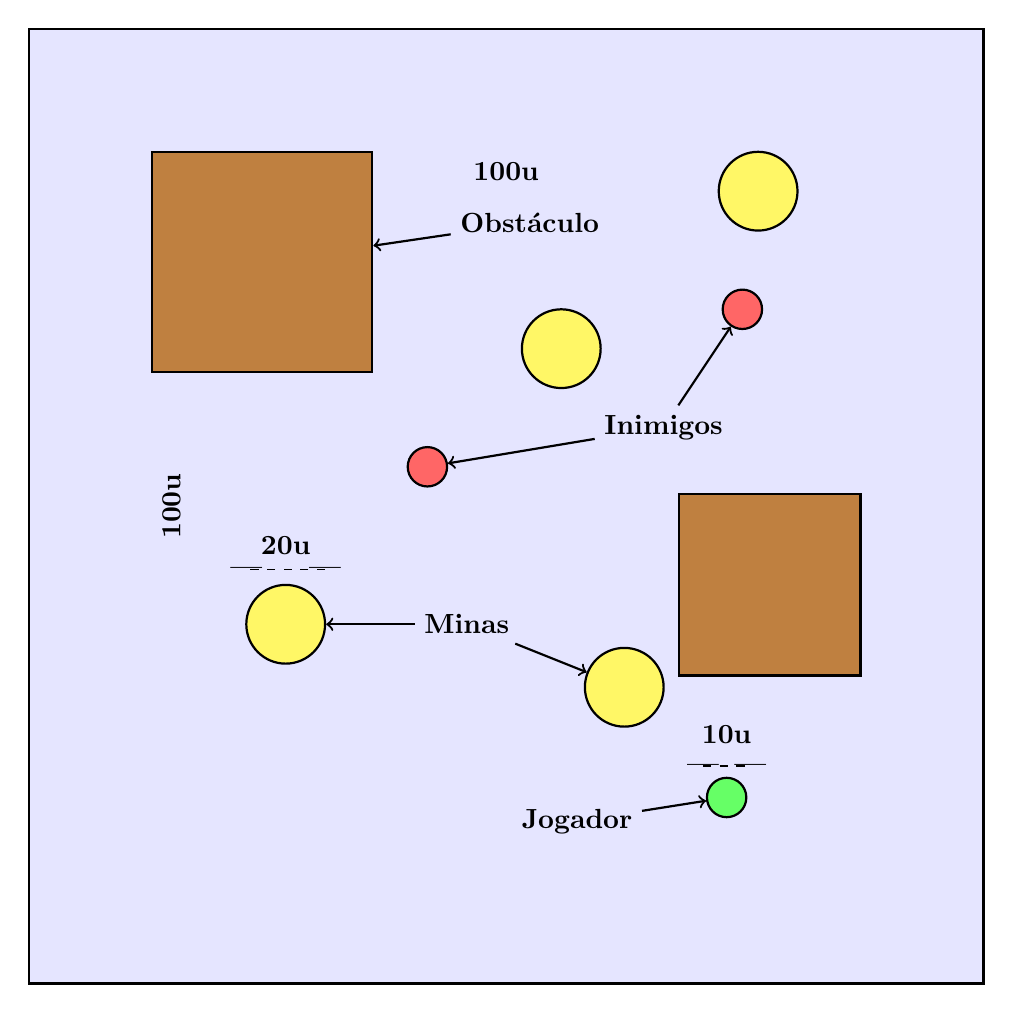
\begin{tikzpicture}[]
	\tikzstyle{sub}=[thick, draw, circle, align=center, minimum size = 0.5cm]					
	\tikzstyle{mine}=[thick, draw, circle, align=center, minimum size = 1cm, fill=yellow!60!white]					
	\tikzstyle{obstacle}=[thick, draw, rectangle, align=center, fill=brown]					
	\node[align=center, fill=blue!10!white, thick, draw, thick, rectangle, minimum height=\columnwidth, minimum width=\columnwidth](tarea)at (0,0) {};
	\node[](a1)at (0, 4.25) {\bf 100u};
	\node[rotate=90](a1)at (-4.25, 0) {\bf 100u};
	
	\node[obstacle, minimum size=2.8cm](obs1)at (-3.1, 3.1) {};
	\node[obstacle, minimum size=2.3cm](obs2)at (3.35, -1) {};
	\node[](tobs)at (0.3, 3.6) {\bf Obstáculo};
	\draw[->, thick](tobs) -- (obs1);

	\node[fill=green!60!white, sub](player)at (2.8, -3.7) {};	
	\node[](tplayer)at (0.9, -4) {\bf Jogador};
	\draw[->, thick](tplayer) -- (player);
	\node[](a1)at (3.1, -3.3) {\bf |};
	\node[](a2)at (2.5, -3.3) {\bf |};
	\draw[-, dashed](2.5, -3.3) -- (3.1, -3.3);
	\node[](a2)at (2.8, -2.9) {\bf10u};
	
	\node[fill=red!60!white, sub](enemy1)at (-1, 0.5) {};	
	\node[fill=red!60!white, sub](enemy2)at (3, 2.5) {};
	\node[](tenemy)at (2, 1) {\bf Inimigos};
	\draw[->, thick](tenemy) -- (enemy1);
	\draw[->, thick](tenemy) -- (enemy2);
	
	\node[mine](mine1)at (-2.8, -1.5) {};	
	\node[mine](mine2)at (1.5, -2.3) {};
	\node[mine](mine3)at (0.7, 2) {};
	\node[mine](mine4)at (3.2, 4) {};
	\node[](tmines)at (-0.5, -1.5) {\bf Minas};
	\draw[->, thick](tmines) -- (mine1);
	\draw[->, thick](tmines) -- (mine2);
	
	\node[](a1)at (-3.3, -0.8) {\bf |};
	\node[](a2)at (-2.3, -0.8) {\bf |};
	\draw[-, dashed](-2.3, -0.8) -- (-3.3, -0.8);
	\node[](a2)at (-2.8, -0.5) {\bf20u};	
	\end{tikzpicture}
\end{figure}
%
\vfill
%
No início do jogo, espalhe os submarinos do inimigo e dos jogadores, assim como possíveis obstáculos no mapa.
Além disso, determine a posição das minas, mas as mantenha em segredo até que sejam ativadas ou detectadas pelo sonar.
Antes de iniciar o jogo, os jogadores podem escolher um dos 3 níveis de dificuldade, que determinam a quantidade de minas e submarinos inimigos, assim como o prêmio recebido em caso de vitória.
%
\\\\
%
\oftable{p{0.2\columnwidth} p{0.35\columnwidth} p{0.4\columnwidth}}
{\accf{Dificuldade} & \accf{Inimgos / Minas} & \accf{Prêmio}}
{
	Fácil 	& 1 / 2 & Matéria negra\ofrow
	Médio	& 2 / 4 & Materia esfregão \ofrow
	Difícil 	& 3 / 6 & Grampo dourado \ofrow
}
%
\clearpage
%
%
%
%
%
%
%
%
%
\includegraphics[width=\columnwidth]{./art/goldsaucer/chocoborace.jpg}
%
\vfill
%
\accf{Corrida de chocobo} é um jogo de corrida cuja entrada custa 2 Gp por jogador. 
Cada jogador é um jóquei na corrida e podem escolher uma das seguintes Chocobos fornecidas pelo parque ou usar alguma própria.
O MJ adiciona e joga com os participantes restantes na corrida até que haja 5 competidores no total.
%
\\\\
%
\oftable{p{0.35\columnwidth} p{0.3\columnwidth} p{0.3\columnwidth}}
{\accf{Chocobo} & \accf{Fôlego} & \accf{Agilidade}}
{
	Eco 	& 4 & 5 \ofrow
	Cinco 	& 5 & 4 \ofrow
	Rex 	& 6 & 3 \ofrow
	Cody 	& 7 & 2 \ofrow
	Jesse   & 8 & 1 
}
%
\vfill
%
Uma corrida consiste em várias rodadas e durante cada uma delas, cada participante realiza um teste de arrancada para determinar a distância percorrida.
Eles somarão continuamente os resultados de seus testes à pontuação final, o primeiro a superar 50 pontos vence.
A pontuação de cada um deles deve ser anunciada ao final de cada rodada e registrada.
Se mais de um participante alcançar a linha de chegada na mesma rodada, aquele com a maior pontuação vence.
O teste de arrancada realizado a cada turno é modificado da seguinte maneira: \ofrow
%
\ofbullet{%
	O resultado de cada arrancada é reduzido pela diferença entre o Fôlego da Chocobo e sua fadiga atual.
	Todos começam com 0 de fadiga e ganham 1 ponto ao final de cada rodada.
	Por exemplo, se uma Chocobo tem fadiga 10 e Fôlego 8, o resultado do teste será reduzido em 2, mas se ela tivesse 10 ou mais de Fôlego, não receberia penalidade alguma.
	Esta redução não pode fazer com que a arrancada caia abaixo de 0.
}
\ofbullet{%
	Antes de cada teste, um participante pode decidir realizar uma ação de disparada.
	Neste caso, ele ganha Vantagem no teste de arrancada, mas também, um ponto de fadiga extra.
	Na corrida, você pode disparar somente uma quantidade de vezes igual à Agilidade da Chocobo.
}
\ofbullet{%
	Os personagens que são particularmente bons em lidar com Chocobos têm Vantagem nos testes de arrancada.
}
%
\\\\
%
Quando a corrida termina, o vencedor rola 1d e recebe o prêmio baseado no resultado.
%
\newpage
%
\oftable{p{0.4\columnwidth} p{0.7\columnwidth}}
{\accf{Resultado} & \accf{Prêmio}}
{
	1 & 10 GP \ofrow
	2 & Pena de Fênix \ofrow
	3 & Matéria de aviso \ofrow
	4 & Elixir \ofrow
	5 & Matéria debandada \ofrow
	6 & Sandália alada
}
%
\\\\
%
%
%
%
%
%
%
%
%
\begin{center} \includegraphics[width=\columnwidth]{./art/goldsaucer/snowgame.jpg} \end{center}
\accf{Jogo de Neve} é um jogo de snowboard que custa 1 GP por jogador. 
Ele funciona com vários jogadores que correm abaixo numa pista de ski tentando alcançar a maior pontuação.
Ela começa em 0, coletar balões a aumenta, enquanto esbarrar em obstáculos, a reduz, por isso a pontuação pode ser negativa.
O jogo tem até 7 rodadas e no começo de cada uma delas, o MJ rola 3d, um dado após o outro, a fim de determinar os objetos nas 3 pistas em frente aos jogadores da esquerda à direita.
A tabela abaixo mostra os possíveis objetos baseados no resultado do dado e seus efeitos, ao se colidirem com eles.
%
\\\\
%
\oftable{p{0.3\columnwidth} p{0.35\columnwidth} p{0.3\columnwidth}}
{\accf{Resultado} & \accf{Objeto} & \accf{Efeito}}
{
	1 - 2 & Nada & -- \ofrow
	3 & Boneco de neve & - 1 ponto \ofrow
	4 & Rocha & - 2 pontos  \ofrow
	5 & Balões vermelhos & + 1 pontos \ofrow
	6 & Balões azuis & + 2 pontos  \ofrow
}
%
\\\\
%\clearpage
%
Depois de aprender sobre os objetos em frente a eles, cada jogador pode decidir entre 1 de 3 ações:\ofrow
\ofbullet{\accf{Mova-se à pista da esquerda ou à da direita:} faça um teste de DF~6, se for bem sucedido, mude uma pista, do contrário, fique na atual.} 
\ofbullet{\accf{Mova das pistas à esquerda ou àdireita:} faça um teste de DF~8, se for bem sucedido, mude duas pistas, do contrário fique na atual.} 
\ofbullet{\accf{Saltar:} faça um teste de DF~8, se bem sucedido, evite o obstáculo a sua frente e ganhe 1 ponto. Se falhar, colida com ele e perca 1 ponto. Você pode usar essa ação mesmo se não haver objetos a frente.} \ofrow
Os personagens que são particularmente bons em coordenação ou têm experiência com snowboards, têm  Vantagem nesses testes. 
Após todas as ações serem realizadas, avalie em quais pistas que cada jogador terminou e com quais objetos colidiram, ou não, para anotar a pontuação antes do inicio da próxima rodada.
Ao fim da 7º rodada, todos os jogadores alcançam a linha de chegada a depender de sua pontuação, cada um deles recebem um dos seguintes prêmios.
%
\\\\
%
\oftable{p{0.4\columnwidth} p{0.7\columnwidth}}
{\accf{Ponruação} & \accf{Prêmio}}
{
	< 3 & Medalha de participação \ofrow
	3 - 4 & Super poção \ofrow
	5 - 6 & Pin de segurança \ofrow
	7 - 8 & PV+ \ofrow
	> 8 & 50 GP \ofrow
}
%
%
\ofpar\\\\
%
%
%
%
%
%
\includegraphics[width=\columnwidth]{./art/goldsaucer/gbike.jpg}
\\\\
\accf{Moto-G} é um jogo de moto em que os jogadores são perseguidos por motociclistas hostis numa auto estrada e têm que lutar para conseguir escapar. 
O jogo pode ser jogado por vários jogadores pelo custo de 1 GP por jogador.
A auto estrada tem 4 pistas e o foco é sempre colocar 3 filas, assim haverá 12 posições no total, onde motociclistas e obstáculos podem ser colocados no momento certo.
A ilustração abaixo mostra como o mapa pode se parecer durante o jogo.
%
%\newpage
%
\begin{figure}[h!]
	\centering
	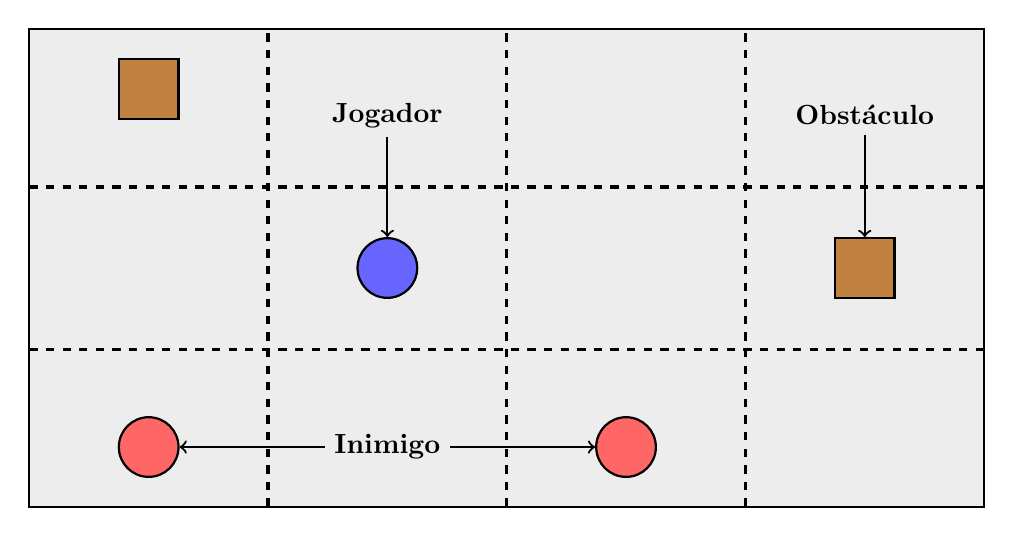
\begin{tikzpicture}[]
	\tikzstyle{biker}=[thick, draw, circle, align=center, minimum size = 0.5*0.125\columnwidth]					
	\tikzstyle{obstacle}=[thick, draw, rectangle, align=center, fill=brown, minimum size=0.5*0.125\columnwidth]					
	
	\node[align=center, thick, draw, thick, rectangle, minimum height=0.5\columnwidth, minimum width=\columnwidth, fill=black!7!white](tarea)at (0,0) {};		
	\draw[very thick, -, dashed](-0.25\columnwidth, -0.25\columnwidth) -- (-0.25\columnwidth, 0.25\columnwidth);
	\draw[very thick, -, dashed](0, -0.25\columnwidth) -- (0, 0.25\columnwidth);
	\draw[very thick, -, dashed](0.25\columnwidth, -0.25\columnwidth) -- (0.25\columnwidth, 0.25\columnwidth);
	\draw[very thick, -, dashed](-0.5\columnwidth, 0.5*-0.17\columnwidth) -- (0.5\columnwidth, 0.5*-0.17\columnwidth);
	\draw[very thick, -, dashed](-0.5\columnwidth, 0.5*0.17\columnwidth) -- (0.5\columnwidth, 0.5*0.17\columnwidth);
	
	\node[fill=red!60!white, biker](b1)at (-0.375\columnwidth, 0.5*-0.375\columnwidth) {};
	\node[fill=red!60!white, biker](b2)at (0.125\columnwidth, 0.5*-0.375\columnwidth) {};
	\node[fill=blue!60!white, biker](b3)at (-0.125\columnwidth, 0) {};
	\node[obstacle](obs1)at (0.375\columnwidth, 0) {};
	\node[obstacle](obs2)at (-0.375\columnwidth, 0.5*0.375\columnwidth) {};
	
	\node[](tobs)at (0.375\columnwidth, 0.16\columnwidth) {\bf Obstáculo};
	\draw[->, thick](tobs) -- (obs1);
	\node[](tplayer)at (-0.125\columnwidth, 0.16\columnwidth) {\bf Jogador};
	\draw[->, thick](tplayer) -- (b3);
	\node[](tenemy)at (-0.125\columnwidth, 0.5*-0.375\columnwidth) {\bf Inimigo};
	\draw[->, thick](tenemy) -- (b1);
	\draw[->, thick](tenemy) -- (b2);
	\end{tikzpicture}
\end{figure}
%
\newpage
%
O jogo funciona em 7 rodadas e durante cada uma delas, em primeiro lugar, todos os jogadores agem e então os motociclistas hostis.
Os jogadores começam com 3 PV e os inimigos com 1 PV, ao ser reduzido a 0 PV, o motociclista é removido do jogo.
Durante um turno, cada um pode fazer um movimento e realizar um ataque:
\vfill
\ofbullet{\accf{Movimento:} mova-se a uma pista à esquera / direita ou uma fila à frente / trás. se a posição não estiver ocupada por um obstáculo ou outro motociclista. Também é possível ativar o turbo da moto. Neste caso, faça um teste de DF~8, se for bem suceiddo, você pode realizar dois movimentos nesse turno, se falhar, não pode se mover. Os personagens que sejam particularmente bons em dirigir veículos recebem Vantagem neste teste}\ofpar
\ofbullet{\accf{Ataque físico:} faça um teste de DF~6, se bem sucedido, um moticiclista que estiver a 1 movimento de distância, sofre 1 ponto de PV.}\ofpar
\ofbullet{\accf{Ataque â distância:} faça um teste de DF~8, se bem sucedido, um motociclista que esteja a 2 ou menos movimentos de distância, sofre 1 PV de dano.}
%
\vfill
%
No início de cada rodada, role 1d para cada jogador que ainda estiver no jogo.
Baseado no resultado, ponha os seguintes itens em qualquer posição aberta à sua escolha: 1-2: nada, 3: motociclista vermelho, 4: motoqueiro azul, 5-6: obstáculo.
No entanto, não ponha qualquer motoqueiro hostil se já houver a mesma quantidade deles que a de jogadores.
Os motoqueiros vermelhos e azuis são controlados pelo MJ e seguem as mesmas regras que os jogadores, mas os vermelhos só podem realizar ataques à distância enquanto os azuis, somente ataques físicos.
Todos os obstáculos seguem as mesmas regras e o MJ é livre para escolher a aparência deles, podendo ser bloqueios ou veículos.
Sempre que um jogador terminar seu turno com um obstáculo na mesma pista em frente a ele, ele tem que fazer um teste de DF~6, se bem sucedido, ele salta o obstáculo, mas se falhar, sofre 1 PV de dano.
Motoqueiros inimigos esquivam de todos eles automaticamente. No fim de cada rodada, todos os motoqueiros ficam em suas posições e todos os obstáculos desaparecem, enquanto são deixados para trás do campo de visão.
Cada jogador que sobreviver até o fim da 7º rodada, ganha o prêmio.
Cada vencedor rola 1d e dependendo do resultado, recebe um dos seguintes prêmios.
%
\vfill
%
\oftable{p{0.4\columnwidth} p{0.5\columnwidth}}
{\accf{Resulto} & \accf{Prêmio}}
{
	1 	 & Suporte de item \ofrow
	2    & 5 GP \ofrow		
	3    & Super Éter \ofrow
	4    & Pena de Fênix \ofrow
	5    & Matéria alerta \ofrow    
	6    & Matéria bomba
}
%
\clearpage
%
%
%
%
%
%\includegraphics[width=\columnwidth]{./art/goldsaucer/proxycatcher.jpg}
%%
%\vfill
%%
%\accf{Proxy Catcher} is a crane game that costs 4 GP to play.
%The game is played by a single player who uses the controls of the machine to navigate a crane and potentially pick a valuable prize from a pile.
%The player only has one chance to lower the crane and grab something.
%To do so, the player makes a check and receives a prize based on the result as listed in the table below.
%However, the game is rigged as the crane has a fixed chance of properly grabbing something.
%Players can perform a DC~8 check to understand that the player skill has barely any influence on the odds of success.
%%
%\vfill
%%
%\oftable{p{0.5\columnwidth} p{0.5\columnwidth}}
%{\accf{Result} & \accf{Prize}}
%{
%	2 - 5 & Nothing \ofrow
%	6 - 7 & Potion \ofrow
%	8     & 5 GP \ofrow		
%	9     & Ether \ofrow
%	10    & Phoenix Down \ofrow
%	11    & 20 GP \ofrow    
%	12    & Counter Materia
%}
%\vfill
%%
%{
%\begin{center}\includegraphics[width=0.7\columnwidth]{./art/goldsaucer/caitsith.jpg}\end{center}
%%
%%
%%
%%
%\newpage
%%
%\includegraphics[width=\columnwidth]{./art/goldsaucer/arena.jpg}
%%
%\vfill
%%
%The \accf{Colosseum} is a battle arena that costs 1 GP per player to participate in.
%All players that want to participate, fight up to 7 groups of monsters together as a party, one after another, on a 10u by 10u battlefield with walls on all 4 sides.
%After the party defeats one group, roll 1d and depending on the result, they receive an additional handicap in each subsequent fight.
%If you roll the same number twice, roll again until you get a handicap that is not active yet.
%The list below shows the 6 possible handicaps, so by time the party reaches the 7th round, all of them will be active.
%%
%\vfill
%%
%\oftable{p{0.15\columnwidth} p{0.75\columnwidth}}
%{\accf{Result} & \accf{Handicap}}
%{
%	1 & You can no longer equip Materia. \ofrow
%	2 & You can no longer use Items.  \ofrow
%	3 & You can no longer equip Accessories. \ofrow
%	4 & You can no longer equip Armor.  \ofrow
%	5 & You can no longer use Limit Breaks. \ofrow
%	6 & You suffer Zombie until you leave the Colosseum (cannot be removed). \ofrow
%}
%%
%\vfill
%%
%After defeating a group, everyone in the party can take an additional turn before the next fight starts.
%At that point, they can also decide to forfeit and collect a prize depending on how many rounds they have completed.
%If the entire party is defeated within a round, they do not receive any prize.
%In any case, the party fully recovers their HP and MP after leaving the Colosseum.  
%The list below shows the possible prizes depending on how many rounds were completed.
%The following page shows the 7 types of monsters encountered from the 1st to the 7th round.
%At the start of each round, place as many of the current round's monster type on the battlefield as there are players.
%%
%\vfill
%%
%\oftable{p{0.4\columnwidth} p{0.75\columnwidth}}
%{\accf{Round} & \accf{Prize}}
%{
%	1 & Potion \ofrow
%	2 & Phoenix Down \ofrow
%	3 & 10 GP \ofrow
%	4 & Lure Materia  \ofrow
%	5 & Rewind Materia \ofrow
%	6 & Protect Bangle \ofrow
%	7 & Genji Gloves \ofrow
%}
%%
%\clearpage
%%
%\ofmonster{Python (Round 1)}{3}{\includegraphics[width=0.2\columnwidth]{./art/goldsaucer/python.jpg}}
%{
%	HP: & \hfill 24 & MP: & \hfill 18\\
%	STR: & \hfill 3 & DEF: & \hfill 1 \\
%	MAG: & \hfill 0 & RES: & \hfill 3 \\
%	AGI: & \hfill 3 & Size: & \hfill M\\
%}
%{\accf{Bite}: 1d DMG \hfill \accf{Immune:}\poison \hfill \accf{Weak:}\earth}
%{	
%	\mtech{Entangle}{6}{0r}{Single}{3u}{The target makes a DC 8 check and suffers 2d damage and Immobile for 1 round upon failure.}{\immobile}		
%}
%%
%\vfill
%%
%\ofmonster{Hecteyes (Round 2)}{4}{\includegraphics[width=0.2\columnwidth]{./art/goldsaucer/hecteyes.jpg}}
%{
%	HP: & \hfill 32 & MP: & \hfill 50\\
%	STR: & \hfill 1 & DEF: & \hfill 2 \\
%	MAG: & \hfill 6 & RES: & \hfill 8 \\
%	AGI: & \hfill 2 & Size: & \hfill M\\
%}
%{\accf{Tackle}: 2d DMG \hfill \accf{Immune:}\sleep \hfill \accf{Weak:}\lightning}
%{	
%	\mspell{Blind}{6}{1r}{Single}{3u}{The target makes a DC 8 check and suffers Blind for 3 round upon failure.}{\blind}		
%	\mspell{Thunder}{4}{1r}{Single}{3u}{You deal 2d lightning damage to the target.}{\ice}		
%}
%%
%\vfill
%%
%\ofmonster{Mantis (Round 3)}{5}{\includegraphics[width=0.23\columnwidth]{./art/goldsaucer/mantis.jpg}}
%{
%	HP: & \hfill 46 & MP: & \hfill 30\\
%	STR: & \hfill 4 & DEF: & \hfill 2 \\
%	MAG: & \hfill 0 & RES: & \hfill 2 \\
%	AGI: & \hfill 3 & Size: & \hfill M\\
%}
%{\accf{Cut}: 2d DMG \hfill \accf{Immune:}\immobile \hfill \accf{Weak:}\fire}
%{	
%	\mtech{Metal Cutter}{4}{0r}{Single}{Weapon}{Make an Attack against the target. If you succeed, the damage dealt ignores the target's DEF.}{}		
%	\mpassive{Leap}{When moving you can jump over enemies and obstacles up to a height of 2u, instead of having to walk around them.}	
%}
%%
%\vfill
%%
%\ofmonster{Griffon (Round 4)}{6}{\includegraphics[width=0.23\columnwidth]{./art/goldsaucer/griffon.jpg}}
%{
%	HP: & \hfill 67 & MP: & \hfill 50\\
%	STR: & \hfill 6 & DEF: & \hfill 3 \\
%	MAG: & \hfill 0 & RES: & \hfill 5 \\
%	AGI: & \hfill 3 & Size: & \hfill M\\
%}
%{\accf{Claw}: 2d DMG \hfill \accf{Immune:}\immobile\blind \hfill \accf{Resilient:}\wind}
%{	
%	\mtech{Feather Shot}{6}{0r}{Single}{4u}{The target suffers 3d wind damage.}{\wind}		
%	\mpassive{Peck}{Whenever you successfully Attack a target he makes a DC 7 check and suffers Blind for 3 rounds upon failure.}
%}
%%
%\newpage
%%
%\ofmonster{Big Horn (Round 5)}{7}{\includegraphics[width=0.23\columnwidth]{./art/goldsaucer/bighorn.jpg}}
%{
%	HP: & \hfill 90 & MP: & \hfill 80\\
%	STR: & \hfill 7 & DEF: & \hfill 5 \\
%	MAG: & \hfill 0 & RES: & \hfill 5 \\
%	AGI: & \hfill 2 & Size: & \hfill L\\
%}
%{\accf{Tackle}: 3d DMG \hfill \accf{Immune:}\poison \hfill \accf{Resilient:}\fire}
%{	
%	\mtech{Charge}{8}{1r}{Single}{10u}{Dash towards the target and deal 3d damage to him. In addition, the target is knocked back by 3u and if he hits a wall, he suffers an additional 3d damage.}{}		
%	\mreaction{Kickback}{Whenever you suffer damage from an enemy within 1u, you can deal 10 physical damage to him and knock him back by 2u.}
%}
%%
%\vfill
%%
%\ofmonster{Golem (Round 6)}{8}{\includegraphics[width=0.23\columnwidth]{./art/goldsaucer/golem.jpg}}
%{
%	HP: & \hfill 130 & MP: & \hfill 100\\
%	STR: & \hfill 9 & DEF: & \hfill 8 \\
%	MAG: & \hfill 0 & RES: & \hfill 6 \\
%	AGI: & \hfill 2 & Size: & \hfill L\\
%}
%{\accf{Fist}: 3d DMG \hfill \accf{Immune:}\poison\sleep\ \hfill \accf{Resilient:}\earth}
%{	
%	\mspell{Quake}{20}{1r}{3u}{7u}{Deal 6d earth damage to everyone in the target area.}{\earth}
%	\mtech{Earth Wall}{12}{0r}{3u (line)}{3u}{You create a 3u tall and wide wall of earth that blocks the path. The wall breaks down after 3 rounds or upon suffering a total of 15 damage.}{}
%}
%%
%\vfill
%%
%\ofmonster{Dark Dragon (Rnd 7)}{9}{\includegraphics[width=0.24\columnwidth]{./art/goldsaucer/blackdragon.jpg}}
%{
%	HP: & \hfill 200 & MP: & \hfill 180 \\
%	STR: & \hfill 10 & DEF: & \hfill 7 \\
%	MAG: & \hfill 9 & RES: & \hfill 8 \\
%	AGI: & \hfill 3 & Size: & \hfill L\\
%}
%{\accf{Bite}: 3d DMG \hfill \accf{Resilient}:\fire\ice\dark \\ \accf{Immune}: All Status Effects}
%{
%	\mtech{Obliterating Breath}{16}{0r}{3u (front)}{3u}{Everyone in the target area makes a DC 8 check and suffers 4d damage as well as Poison and Blind for 3 rounds upon failure.}{\poison \blind}{}
%	\mspell{Dark Flare}{30}{2r}{Single}{5u}{You deal 6d+20 dark damage to the target.}{\dark}
%	\mpassive{Tail Whip}{Whenever you Attack, you can choose to target all enemies within 1u at once.}	
%}	
%
%\clearpage
%\ofsection{Introduction}
%
\ofquote{"Names don't matter. What's important is how you live your life."}{Ramza Belouve}\\\\
%
This book is an updated version of the original Final Fantasy Tactics worldbook released in 2017.
The original version also included specific rules for the Final Fantasy Role Playing Game 4th Edition~(\textbf{FFPRG~4e}), that are improved in this update.
Additionally, this book includes specific rules for \textbf{Omega~Fantasy}, which is another game system that aims to recreate the feeling of the Final Fantasy series.
Nevertheless, the vast majority of the content and ideas presented in this worldbook are system agnostic and thus should be applicable to other tabletop RPGs. 
%
\\\\
%
\textbf{Final Fantasy Tactics}~(FFT) is a spin-off title in the main Final Fantasy series. 
Unlike most spin-offs, however, it has managed to be a great game on its own, having received universal acclaim upon its release, and critical opinion of the game has improved further over time. 
It is the first game of the Final Fantasy Tactics series and was released in Japan in June 1997 and in the United States in January 1998. 
The game combines thematic elements of the Final Fantasy video game series with a game engine and battle system unlike those previously seen in the franchise. 
In contrast to other 32-bit era Final Fantasy titles, Final Fantasy Tactics uses a 3D, isometric, rotatable playing field, with bitmap sprite characters.
For many Final Fantasy players, this represented their first foray into the Strategy RPG genre, with its own quirks and conventions established by several other games that came before, like Shining Force, the Langrisser series or Tactics Ogre. 
For this reason, and to celebrate the 20th anniversary of the original Japan release of this cult classic, this worldbook was born.
%
\\\\
%
Final Fantasy Tactics uses a three-dimensional isometric battle grid. 
This difference in functionality led to a game type that was more akin to chess than the traditional back and forth linear combat of previous Final Fantasy games. 
Instead of having six characters that were all-essential to the plot, and joined your party over a period, you had a singular main character that would occasionally be joined by story important characters that would depart and rejoin you when the plot demanded they do so. 
The bulk of your adventuring party was usually made up of interchangeable, nondescript characters whose appearance shifted radically depending on what \textbf{job class} they were.
The progression of job classes in this system is quite similar to that of older Final Fantasy games, in that there were several job classes to choose from, but fundamentally different in how certain
job classes were unlocked. 
Instead of obtaining crystals that granted certain job classes automatically, you were given two starting job classes and expanded upon them. 
Your job progress reveals others, and if you took multiple levels in multiple jobs, your amalgamated experience in those two jobs might reveal another job class that was unique. 
This system involved a lot of job class switching and of course, a small amount of class mapping to determine which job classes unlocked another.
%
\\\\
%
The story of Final Fantasy Tactics revolves around the aftermath of \textbf{The 50 Year War}. 
The kingdom of \textbf{Ivalice} is rife with political and economic discrepancies between the upper and lower class. 
This problem is compounded by the recent death of the king, whose only heir is an infant, and the need for a regent to rule in his place. 
The people are stuck between Prince Goltana, and Prince Large, known as the Black and White Lion respectively.
This leads into the main plot of the game, known as \textbf{The Lion War}, in which you take on the role of \textbf{Ramza Beoulve}. 
As the name implies, The Lion Wars were conflicts between the two princes in their attempt to become the ruling regent. 
Ramza is a young noble who takes part in many exploits of the war, discovers hidden corruption and machinations within the most powerful church in the lands, and comes to understand the plight of the common peoples. 
He was a decisive factor in the resolution of the war but was actively erased from history.
%
%
\\\\
\ofquote{"The best ways, don't always lead to the best results."}{Delita Hyral}
\vfill
\includegraphics[width=\columnwidth]{./art/images/everyone.jpg}
%
\clearpage
%
%
\ofsection{History of Ivalice}
%
\ofaccent{The Beginning (10000 B.C. -- 2000 B.C.)}\\
During this period of time, estimated from 10000 to 2000 B.C. on the Ajorian Calendar, the majority of humankind lived on the southwestern coast of what years later would become Kaladis. 
Most of the people of these times were simply tribes of hunter-gatherers. 
As the age neared its close, however, metallurgy was developed as well as basic magic study. 
Unfortunately, there are extremely few records from this period, partly in thanks to a lack of a written language, which was first developed during the age of the Ronan Empire, although there are some rare ruins left behind that have been found in remote parts of Kaladis.
During this period, the countries that would later become Kaladis and Mizuno were first settled. Ivalice, Romanda, and Ordalia were first settled during the Ronan Empire.
%
\\\\
\includegraphics[width=\columnwidth]{./art/images/ovelia.jpg}
\\\\
%
\ofaccent{The Ronan Empire (2000 B.C. -- 700 B.C.)}\\
History dates the first true civilization as the Ronan Empire; an empire that grew from a humble farm village near Zeltenia to a huge empire that spanned most of what would become Ivalice and parts of Romanda and Ordalia near its end, roughly estimated between 700 and 600 B.C.. 
Not much is known about this mysterious empire save that it excelled at the use of magic even compared to the level used by the most powerful of today's magicians. 
Even more mysterious is what caused its downfall. 
The Ronan Palace, the center of the empire, was up until its discovery during the Lion Wars a myth in and of itself. 
Several important ruins originated from this era including Matoya's cave, the Tower of Babel, Mirage Tower, and of course the \textbf{Ronan Palace}. 
The Ronan Empire was the first country to develop a written language with Mizuno soon following within its own language known as Nihonjin.
%
\\\\
\includegraphics[width=\columnwidth]{./art/images/tree.jpg}
\\\\
%
\ofaccent{The Age of Myth (700 B.C. -- 50 B.C.)}\\
Following the downfall of the Ronan Empire, the territories splintered into four separate countries: Melmond, the Baron Kingdom, the Kushuka Kingdom, and the Palamecian Empire. 
Like the Ronan Empire, these four nations covered Ivalice and began making inroads into the areas that would become Romanda and Ordalia in later years. 
This period is largely known as the age of myth in part due to the amount of fantastic ruins that were left behind as well as the level of technology developed.
\textbf{Baron Kingdom} was a kingdom whose military might rivaled many of the other nations during the age of myth. 
Baron supported a large number of elite knights as well as a well-known navy of airships. 
Baron covered much of what would become Gallione, Fovoham, and western Lesalia.  
Compared to its neighbors, the \textbf{Kushuka Kingdom} was a center of trade where traders from other countries would come to sell their wares. 
Unfortunately, for the country itself, its nobility ruled with harsh hand with little concern for their people.
After years of abusing the coffers of their nation, the royal family was dethroned by a huge revolution. 
On a modern map, Kushuka would occupy much of central Lesalia and most of Zeltenia.
Like its neighbors, the \textbf{Palamecian Empire} had a specialty, namely technology. 
It was the first to develop airships and maintained a fleet that was a fair equivalent of Baron's navy. 
In addition to its airships, Palamecia also first developed guns that used magical ammunition as well as its "war golems", powerful robots that were used as first line soldiers and guards. 
The empire covered what would become Lionel. 
Many historians believe that its capital is deep below Goug Machine City. 
Palamecia was also the first to develop steam-powered devices and were the first to develop the science of magitek, which involves the fusing of magic and machine.
\textbf{Melmond} was a secluded nation far to the east in what would later become southern Ordalia. 
More than other countries, Melmond embraced the study of magic in full and supported many academies dedicated to teaching the arcane arts to interested students. 
Other studies such as history, philosophy, and literature were also popular among Melmond people. 
Unfortunately, Melmond was considered by many of its neighboring countries to be working with the forces of Lucavi because of their magical might.
Like the Ronan Empire before them, all four kingdoms of the age of myth were destroyed by unknown circumstances. 
The \textbf{Zodiac Brave Story} first emerged during this era. 
For those that do not know it, the Zodiac Brave Story is the tale of an evil king who called on the powers of Lucavi, around the year 500~B.C..
Lucavi killed the king and caused great havoc throughout the world. 
In the end, a small group of 12 heroes banded together and used the sacred zodiac stones to become the Zodiac Braves. 
The Zodiac Braves were able to defeat Lucavi and supposedly restored order. 
Following the defeat of Lucavi, the \textbf{Holy Ydoran Empire} was founded, emerging from the ruins of the old Baron Kingdom.
The empire waged several wars, eventually defeating and conquering both Palamecia and Melmond.
%
\vfill
\includegraphics[width=\columnwidth]{./art/images/delita2.jpg} 	
\pagebreak\\
\includegraphics[width=\columnwidth]{./art/images/agrias.jpg}
\\\\
%
\ofaccent{The Life \& Death of St.~Ajora (50 B.C. -- 1 B.C.)}\\
The Ajorian Calendar begins its first year with the death of \textbf{St.~Ajora} and the beginning of the \textbf{Cataclysm}. 
By the time Ajora Glabados came, three of the four kingdoms of the age of myth had been conquered by the Holy Ydoran Empire, and the Kushuka Kingdom was the only other state to resist the power of its neighbor. 
The lands that once were Melmond laid abandoned and desolate, as refugees from the Jihads that would follow the rise of the Glabados Church would only resettle them several centuries later.
When Ajora Glabados was young, one day he sprang up, walked to a well, and prophesized that "soon, a calamity will befall this land. 
I am now sealing this well, and no one can drink from it." Several days later, the "Black Death" plagued Zeltenia. 
The people who drank from the contaminated well water fell ill and died one after another.
However, only the families that believed Saint Ajora's words survived and did not fall to disease. 
Since then, Saint Ajora became worshipped as "The Miracle Child" or "The Son of God".
Soon after these events, word of a new messiah spread, who would lead Ivalice out of the chaos born from years of war. 
By the time Ajora had reached 18 years old, he had already gained a devoted community of followers. 
Much like in earlier years, another ambitious king attempted to summon Lucavi. 
The emperor had created an army of immense size in the hopes of securing all of Ivalice under the Holy Ydoran Empire’s control. 
Once again, a new group of Zodiac Braves was created united by St.~Ajora to defeat the new Lucavi.
Despite his growing widespread fame, Ajora had made many enemies. 
The Holy Ydoran Empire feared Saint Ajora's rise to power; they feared his preaching of the coming of God. 
The \textbf{Clergy of the Pharism} faith was the predominant religion and even though they had great influence, the clergy feared Saint Ajora's power. 
The conclusion is obvious.
Saint Ajora was captured with a secret tip from Germonik, Ajora's 13th Apostle. 
Saint Ajora was executed at the Golgollada execution site. 
However, Saint Ajora was the "Son of God". 
God's anger struck at Pheisias, and the Cataclysm began, a series of seismic and volcanic events that shocked the world for the next 25 years.
The Cataclysm is often assumed to be the cause behind the loss of Ivalice's most advanced technologies, though the game never outright states this. 
It also destroyed at least two races, the "winged ones" (possibly the aegyl), the moogles (as told in the Siedge Weald) and the Clockwork City of Goug, and if the Ivalician myth is true, threatened humanity, leading some to believe it is responsible for the disappearance of the non-human races from Ivalice. 
The sinking of Mullonde, involving the drowning of an entire state of the Ivalician peninsula, also relates to it. 
The Cataclysm created the Floating Continent, and destroyed Eureka and of the Fortress of Trials. 
According to legend, the Hero-King Mesa saved humanity from its effects.
%
\\\\
\includegraphics[width=\columnwidth]{./art/images/delita.jpg}
\\\\
%
\ofaccent{Rise of Gloabados Church (25 A.C -- 1112 A.C.)}\\
Following the death of Saint Ajora, his remaining apostles established a new church under his name: the \textbf{Glabados Church}, using its namesake's exploits.
Soon after its establishment, it was able to cooperate with warring nations that sprung after the cataclysm and subsequent collapse of the Holy Ydoran Empire on a working peace treaty that set up the \textbf{Atkasha} family as the rulers of Ivalice. 
As part of the peace treaty, Limberry was assimilated into Ivalice. 
Despite the end of pen warfare among the remaining nations, a new cold war developed between the remaining followers of the Fara Clergy and the newly formed Glabados Church.
As Pharism was weakened thanks to the tragedy that led to the destruction of the Ydoran Empire, the Glabados church had no trouble forcing the Phara Clergy and its remaining followers from Ivalice. 
The remaining Phara followers would, slowly over the next 300 years, help create the nation of Ordalia to the east.
The Glabados Church during the first 1000 years of its existence was very powerful, to say the least.
Thanks to its iron handed fist, it helped create several different splinter factions of the Glabados religion, including the Argades church, which would later become the official religion of the Romanda Empire.
%
\\\\
\includegraphics[width=\columnwidth]{./art/images/luso.jpg}
\\\\
%
\ofaccent{The Fifty Years War (1113 A.C -- 1163 A.C.)}\\
By 1113, King Denamda II ruled Ivalice, while King Devanne III ruled its neighboring kingdom, Ordalia. 
Three knightly orders defended Ivalice: the Order of the Northern Sky Knights, led by Ramza's father, \textbf{Barbaneth Beoulve}, the Order of the Southern Sky Knights led by \textbf{Cidolfus Orlandeau}, and the Order of the Eastern Sky, under the leadership of \textbf{Goffard Gaffgarion}. 
Gustav Margriff and \textbf{Wiegraf Folles} served within the Order of the Northern Sky.
Strife erupted at Zelmonia, a once independent province near to Ivalice's border and now under Ordalian rule. 
About a century ago, Ordalia invaded and assimilated Zelmonia. 
Ivalice had secretly provided means to weaken Ordalia; however, the Zelmonian nobles decided to petition for King Denamda's direct intervention. 
King Devanne III died without naming a successor. 
His cousin Varoi VI was named as successor, but King Denamda II proclaimed himself as rightful heir, being Devanne's uncle, and declared war against Ordalia.
King Denamda II led the Ivalice army towards the Ordalian capital of Viura. 
On their way, knights of the three Orders fought valiantly, winning battle after battle.
As they were reaching the Ordalian border, King Denamda II fell ill and died soon after, never able to return to his kingdom. The Ivalician army became lost and confused due to their leader's death and Ordalia used that as an opportunity to strengthen its army and defend the borders. 
%
\begin{center}
	\includegraphics[width=0.56\columnwidth]{./art/images/cid.jpg}
\end{center}
%
The war raged fiercely, reaching a stalemate. 
A successor to Denamda II, Denamda III, was hastily enthroned to replace his father.
During the stalemate, Romanda's armies crossed the Rhana Strait in an invasion upon Ivalice. 
Romanda was a military nation ruled by a blood relative of King Varoi VI. 
King Denamda IV and his Ivalician army held off the invasion through the aid of Fovea’s ruler, Grand Duke Gerrith Barrington, and his assassination squad Khamja.
After three years of fighting, Romanda retreated. 
King Denamda IV was a fearless warrior who personally led his armies in battles against the combined forces of Romanda and Ordalia. 
The outbreak of Black Death within Romanda also led to their retreat.
With Romanda's retreat, Ivalice continued with the war against Ordalia.
Denamda IV died suddenly, believed to be assassinated. 
He was succeeded by King Ondoria Atkascha III, although the king was a weak-willed man and unfit to rule, and all his decisions being made by \textbf{Queen Louveria}.
Ordalia's ruler Varoi VI also died, and was replaced by Prince Lennard. 
Due to Ondoria's weakness, Ordallia forced Ivalice to cease fighting.
The last battle between Ivalice and Ordallia took place in Zeltennia, and though the Knights of the Orders fought bravely, Ordallia won and occupied the province. 
Ivalice and Ordallia agreed to a mutual peace treaty, though whispers persist that in reality, Ivalice had surrendered.
After the Fifty Years' War, Ivalice suffered a great loss as the people harbored ill feelings and dissatisfaction to the nobles and the royal family who placed them in the meaningless war. 
Farmers staged riots and revolted, and many turned banners to join the \textbf{Corpse Brigade}.
Ivalice's economy suffered, as payments could not be made to the knights who had fought in the war due to the spending on weapons and defenses. 
Many were discharged from the army, and with less food and little money, there was high unemployment and disloyalty to the ruling factions grew.
King Ondoria's two sons died, and the king adopted his younger sister, \textbf{Princess Ovelia}, as his daughter. 
Soon after, Queen Louveria gave birth to Prince Orinus, causing a conflict over who should become King Ondoria's successor, setting the stage for the War of the Lions.
Rumors spread of King Ondoria's failing health. 
Since his collapse during Prince Orinus' birthday celebration, it became obvious that he was on the brink of death. 
His advisers, the Board of Chamberlains, delivered news that the king was getting better, but the people knew the truth. Soon rumors surfaced that Queen Louveria and other nobles had argued over his successor.
Goffard Gaffgarion was dismissed from the Eastern Sky, and Gustav from the Northern Sky, both on charges of misconduct during the war. 
Gaffgarion turned to the life of a mercenary, claiming allegiance to the highest bidder.
%
\\\\
\includegraphics[width=\columnwidth]{./art/images/belouve.jpg}
%
\ofaccent{The War of the Lions (1164 A.C -- 1166 A.C.)}\\
The War of the Lions was fought between the Order of the Northern Sky Knights of \textbf{Duke Larg} under the banner of the White Lion, and the Order of the Southern Sky Knights of \textbf{Duke Goltanna} under the banner of the Black Lion. 
King Ondoria Atkascha III died due to the Black Death and his heir, Prince Orinus, was only two years old. 
A regent was sought to rule in the prince's place, and both dukes who were decorated generals in the Fifty Years' War were nominated as regent.
One of the main reasons behind the War is the rift between Queen Louveria and the nobles of Ivalice. 
Queen Louveria was regarded as a power-mad queen who desired her offspring on the throne so that she may rule the kingdom. 
The Council of Nobles, out to stop her from asserting influence onto the kingdom, appointed Duke Goltanna as their preferred candidate for the regency.
%
\\\\
\includegraphics[width=\columnwidth]{./art/images/cover.jpg}
\\\\
%
The first major battle of the War of the Lions, the Battle of Lesalia Plain, was a massive assault of Chocobo Knights from Gallionne on the plains south of the Royal City of Lesalia, where the royal palace is built. 
The Southern Sky was driven out of the city and forced to their strongholds at Fort Besselat and Limberry Castle. 
The victory lead to Southern plans mostly revolving around an attack on Lesalia, by sending an army led by Cidolfus Orlandeau to take the city, though it was driven away.
Further Southern attempts to attack Lesalia culminated in the Battle of Groffovia, fought on the plains between Limberry, which was generally pro-Southern, and Lesalia proper. 
The battle was inconclusive, but within three months casualties reached 40,000, sapping what little public support the war had.
Around this time, Queen Louveria and Chancellor Glevanne were accused of abducting Princess Ovelia to allow for Duke Larg's ascendancy to the throne. In addition, famine overtook Zeltennia, Limberry, Galionne and Fovoham due to a drought, causing mass starvation among civilians.
The losses sustained by the Southern Sky are worsened by the Battle of the Fusse Plains, in which Marquis Elmdore was killed by a stray arrow. 
He was possessed by the Lucavi \textbf{Zalera}, and fought for the Knights Templar at the Battle of Riovanes Castle.
Despite the death of countless soldiers, the war reached a stalemate.
%
\\\\
\includegraphics[width=\columnwidth]{./art/images/riovanes.jpg}
\\\\
% 
The Northern Sky planned to make an all-or-nothing attack at Fort Besselat, planning to take it and use it as a base from which they could wage total war against Southern food supply.
The War's decisive battle was the Battle of Fort Besselat, in which Ramza Beoulve intervened by opening the garrison's sluice, bringing the battle to an indecisive halt. 
Barich Fendsor, one of the Knights Templar, released Mossfungus poison into the air, severely weakening both sides. 
In the confusion, both Dukes were murdered by their respective traitors, Larg by \textbf{Dycedarg Beoulve} and Goltanna by \textbf{Delita Heiral}. 
As originally planned, the Church offered mediators. 
Despite the loss of both Order's leaders, their armies were still strong and refused the idea. 
This may be because of Ramza's intervention, whereas without it, both sides would have suffered major losses if the sluice were not opened.
Ramza Beoulve traveled with his companions to Orbonne Monastery to stop the Knights Templar and the Lucavi's plot for \textbf{Ultima's resurrection}. 
Killing the Church's forces that dared to stop them, they are teleported to the Airship Graveyard beneath the Necropolis of Mullonde and destroyed Ultima, the High Seraph, who wished to destroy Ivalice. 
Their own fate after that is a mystery.
The war finally ended with the two sides crippled. 
With the two dukes killed, Queen Louveria imprisoned in Fort Besselat, High Confessor Funebris murdered, Dycedarg slain, and Orlandeau missing and believed dead, Delita Heiral exploited the situation by claiming that he rescued Princess Ovelia, marrying her to become King of all Ivalice.
The Church of Glabados engineered the War so that it may take the center stage after both sides were weakened due to exhaustion. 
The High Confessor Marcel Funebris, wishing for the Church to gain power over the land, secretly supported both sides and assisted in their plots for the throne. 
The Church planned to destroy the two Lions from the inside and used the Zodiac Stones to strengthen the Church's military power.
%
\begin{center}
\includegraphics[width=0.85\columnwidth]{./art/images/ramza.jpg}
\end{center}
\vfill
\ofquote{"Your actions have meaning only if they hold true to your ideals."}{Ramza Belouve}\\\\
%
\ofaccent{The Glabados Schism (1167 A.C. -- 1250 A.C.)}\\
By 1171, the Glabados Church executed \textbf{Orran Durai} as a traitor after writing the Durai Papers. 
This caused unrest among several ordained priests, and one of them, Karling Nox, initiated a movement in Limberry which called for reformation within the Church, seeking, in his words, a “return to St.~Ajora’s true ways”. 
%
\pagebreak\\
\includegraphics[width=\columnwidth]{./art/images/chocoborider.jpg}
\vfill
%
This rippled through Ordalia and several of the eastern provinces of Ivalice, and after the Church declared Nox’s status as a heretic, the priest started to gather a sizable following. 
Sensing the opportunity to seize lands and riches from the church, several barons and counts declared their conversion to this new interpretation of Ajoran faith, and gave shelter to the new converts.
Weakened by the events of the Lion War, Glabados was unable to prevent the rise of the self-proclaimed Ajorans, and this religious divide kept growing for the next 80 years. In contrast, the Heiral dynasty's rule proved to be quite unsuccessful in keeping the power centralized, and had to make several concessions to the nobility to maintain its position as the Ivalice King.
These concessions increased the decentralization of the kingdom, empowering the local lords.
By 1240, the religious tensions had turned into violence, with hostilities between Glabados and Ajoran followers leading to several small-scale skirmishes, and culminating with the 1243 massacre of Yardrow, where an angry mob killed a congregation of 500 Ajoran faithful during a religious ritual. 
This sprung several mutual defense treaties between nobles, creating both the \textbf{Glabados League}, led by the Grand Duke Rudolph Barrington of Fovoham, and the \textbf{Ajoran League}, led by Marquis Henry Elmdore of Limberry. 
The creation of the two leagues only further increased the tension, but for the next seven years, peace reigned inside Ivalice.
In 1250, following a severe disease, king Luther Heiral went into a comatose state. 
His nephew, Paul Heiral, who was a fervorous devout of the Glabados faith, was designated as Regent. 
Fearing to be persecuted by its religious beliefs, the Ajoran League voted for a preemptive war against the Regent, intending to replace him with another noble who is more sympathetic with the Ajoran faith. 
In response, the Glabados League rallied their troops and this plunged Ivalice into civil war.
%
%
\clearpage
%
%
\ofsection{Timeline}
%
\oftablewide{p{0.3\columnwidth} p{1.6\columnwidth}}
{\ofaccent{Year} & \ofaccent{Important Events}}
{
	< 2000 B.C.& First settlements of hunter-gatherers form. Metallurgy and magic are discovered.\ofrow
%
	\textasciitilde 700 B.C.  & The Ronan Empire, which ruled somewhere in the world from the Ronan Palace, is wiped out by a mysterious disease. \ofrow
%
	\textasciitilde 600 B.C.  & The Ronan Empire splits into 4 countries: Barron Kingdom, Kushuka Kingdom, the Palmecian Empire and Melmond.
			     The level of technology and military develops rapidly.\ofrow
%
	\textasciitilde 500 B.C.  & Lucavi ravage the world.
	A great hero appears leading his twelve companions, each bearing a stone, and they become known as the Zodiac Braves. 
	They defeat the Lucavi. The Holy Ydoran Empire rises from the ashes of the destroyed Baron Kingdom. \ofrow
%
	\textasciitilde 200 B.C.   & The Holy Ydoran Empire conquers the Palmecian Empire and Melmond. 	
	The Orbonne Monastery is built. \ofrow
%
	50 B.C.	  & Saint Ajora is born in Bervenia. \ofrow
%
	22 B.C.	  & Saint Ajora is sent as a spy to the Holy Ydoran Empire and starts preaching about the coming Paradise and gathering Zodiac stones in secret. In total, Ajora gains 13 disciples first of which is Balias, last Germonik who was actually a Ydoran agent. \ofrow
%
	1 B.C.    & Saint Ajora is hanged at Golgollada Gallows by the Holy Ydoran Empire. A disaster sinks parts of Mullonde, forms the Black Coral Sea.\ofrow
%
	\ofaccent{0}  & The Cataclysm occurs. Moogles and winged people are wiped out immediately, along with several flourishing civilizations. The Hero-King Mesa Ricksen saves humanity. The Holy Ydoran Empire is destroyed.\ofrow
%
	25 A.C.   & The remaining disciples of Saint Ajora form the Glabados Church, which establishes itself as the mightiest power in Ivalice for many centuries.\ofrow
%
	150 A.C.  & The city of Yardrow is established.\ofrow
%
	\textasciitilde 300 A.C. & The Glabados Church extends its influence through many splinter factions. They drive the Phara Clergy out of Ivalice who go on to help the creation of Ordalia.\ofrow
%
	610 A.C.  & House Atkascha unifies seven warring kingdoms, establishing the Kingdom of Ivalice.\ofrow
%
	1014 A.C. & The kingdom of Ordallia annexes the independent state of Zelmonia.\ofrow
%
	1086 A.C. & Marcel Funebris is born. \ofrow
%
	1108 A.C. & Druksmald Goltanna, son of the Duke Goltanna and cousin of Ondoria III, is born. Cidolfus Orlandeau, son of Count Orlandeau, is born.\ofrow
%	
	1111 A.C. & Zalmour Lucianada is born.\ofrow
%
	1112 A.C. & Goffard Gaffgarion is born. Alphonse Delacroix is born.\ofrow
%	
	1113 A.C. & King Devanne III of Ordallia dies without naming a successor. King Denamda Atkascha II of Ivalice proclaims himself heir of Ordallia and declares war. The Fifty Years' War starts.\ofrow
% 
	1113 A.C. --\newline1136 A.C & Ivalician forces march on Zelmonia and conquer it. King Denamda II dies on the march of Ivalician forces towards Viura, the capital of Ordallia. Denamda Atkascha III is crowned king of Ivalice. Battles between Ivalice and Ordallia continue on Ordallian ground for these few decades while King Varoi VI of Ordallia tries to push Ivalician forces away from Zelmonia.\ofrow
%
	1117 A.C. & Gerrith Barrington, son of Grand Duke Barrington, is born.\ofrow
%
	1127 A.C. & Bestrald Larg, son of the Duke Larg and relative of Ondoria Atkascha III, is born. Dycedarg Beoulve, first son of Lord Barbaneth Beoulve, is born.\ofrow
%
	1129 A.C. & Messam Elmdore, son of Marquis Elmdore, is born. Gustav Margriff is born. Ondoria Atkascha III, son of Denamda Atkascha IV, is born. \ofrow
%
	1133 A.C. & Bestrald Larg and Dycedarg Beoulve become friends.\ofrow
%
	1134 A.C. & Wiegraf Folles is born.\ofrow
%
	1136 A.C. & Zalbaag Beoulve, second son of Lord Beoulve, is born.\ofrow
}
%
%
\clearpage
%
%
\oftablewide{p{0.3\columnwidth} p{1.6\columnwidth}}
{\ofaccent{Year} & \ofaccent{Important Events}}
{
%	
	1137 A.C. & King Varoi VI of Ordallia succeeds in pushing Ivalician forces back to Zelmonia, a decades-long period of Zelmonian battles follows between Ivalice and Ordallia. Louveria Larg, daughter of Duke Larg, is born.\ofrow
%
	1139 A.C. & Romandan forces invade Ivalice via the Rhana Strait. Ziekden Fortress is built.\ofrow
%
	1140 A.C. & Orran Durai is born.\ofrow
%
	1142 A.C. & Ivalice regains control of Riovanes Castle from the Romandan invaders. Romandan army withdraws from Ivalice due to ferocity of resistance from King Denamda IV and appearance of Black Death at home.\ofrow
%	
	1144 A.C. & Count Cidolfus Orlandeau becomes friends with Duke Druksmald Goltanna. Agrias Oaks is born.\ofrow
%
	1147 A.C. & Duke Bestrald Larg becomes general of the Order of the Northern Sky.\ofrow
%
	1148 A.C. & Delita Heiral is born.\ofrow
%
	1149 A.C. & Ovelia Atkascha, daughter of King Denamda IV, is born Alma Beoulve, fourth child of Barbaneth Beoulve, is born. Tietra Heiral is born. \ofrow
%
	1155 A.C. & Zalbaag Beoulve succeeds the position of Lord Commander of the Order of the Northern Sky after his father. The parents of Delita and Tietra
	Heiral die to the Black Death. Lord Beoulve takes custody of the two children. The parents of Marach and Rapha Galthena are killed. The two wander a while as orphans until Grand Duke Barrington takes them in.\ofrow
%
	1156 A.C. & King Denamda Atkascha IV of Ivalice dies of either illness or murder. Ondoria III is crowned 18th king of House Atkascha. Prince Lennard of Ordallia advances through Zelmonia and invades Zeltennia, and may have reached as far as Limberry.\ofrow
% 
	1157 A.C. & King Ondoria III marries Louveria Larg and she becomes the queen.\ofrow
%
	1161 A.C. & King Ondoria III's second-born son dies shortly after birth.\ofrow
%
	1162 A.C. & Ovelia Atkascha is adopted by King Ondoria III. Orran Durai's father is killed in Count Orlandeau's service, the count adopts him.\ofrow
%
	1163 A.C. & Prince Orinus Atkascha, third son of king Ondoria III, is born. Ramza Beoulve enters the Royal Military Akademy at Gariland. Lord Barbaneth Beoulve dies of poison. Delita Heiral enters the Royal Military Akademy at Gariland. Goffard Gaffgarion is expelled from the position of division commander of the Order of the Eastern Sky for brutality. Veteran soldiers that fought in the ranks of the Dead Men are dismissed without pay, they protest by forming the Corpse Brigade.\ofrow
%
	1164 A.C. --\newline1166 A.C. & After King Ondoria III dies, a dispute about his heir sparks the War of Lions, with the Order
	of the Northern Sky Knights of Duke Larg on the one side and the Order of the Southern Sky Knights of Duke Goltanna on the other. 
	Both are killed by the traitors Dycedarg and Delita respectively. Queen Louveria is imprisoned.
	Ramza Belouve prevents a massacre at the decisive Battle of Fort Basselat and then travels with his companions to prevent the resurrection of Ultima by the Lucavi. The war ends with both sides crippled and most of the important personalities of the period dead.
	\ofrow
%
	1166 A.C. & Delita Heiral marries Ovelia Atkascha and is crowned king of Ivalice. The Glabados Church exploits the situation to regain power.
	\ofrow
%
	1171 A.C. & Orran Durai writes the Durai Papers, and is executed as a traitor by the Glabados Church.\ofrow
%
	1173 A.C. & Karling Nox writes his thesis for Church reformation, and is branded as a heretic. Several nobles of Ordalia and Eastern Ivalice converts to the new Ajoran faith.\ofrow
%
	1243 A.C. & 500 Ajoran faithuls are massacred at Yardrow. The Ajoran league is founded. The Glabados league is founded.
	Tensions increase at first, but peace settles for a while.
	\ofrow
%
	1250 A.C. & Paul Heiral, a Glabados devout, becomes Regeant after his father falls into a coma. 
	Fearing persecution, the Ajoran League preemptively declares against him, starting the Schism War.\ofrow
}
%
%
\clearpage
%
%
\ofsection{Geography of Ivalice}
%
\ofimagewide{\includegraphics[width=\textwidth]{./art/images/map.jpg}} 	
%
\ofaccent{\large Fovoham} is a territory in the northernmost part of Ivalice. 
Ruled by Grand Duke Rudolph Barrington, it is separated from the military nation of Romanda by the Rhana Strait. 
Fovoham played an important role in deterring the Romandan invasion in the Fifty Years' War, thanks to the Grand Duke and his assassin squad Khamja. Nowadays, it is the main force behind the Glabados League, and some even say that the Royal Regent, Paul Heiral, is nothing more than a puppet for the
Grand Duke.
\textbf{Riovanes Castle} is the home and stronghold of Grand Duke Barrington. 
This castle is distinguished by its Romandan-style towers.
Its position enables not only a great defensive position but also control of all the trade that flows through northern Ivalice, as Mt.~Bervenia serves as natural barrier for the movement of goods and armies.
\textbf{Walled City of Yardrow}, also known as Yardrow Fort City is located east of Riovanes Castle and north of the Royal City of Lesalia. It is a fortress city with some ten centuries of history, protected by thick stone walls built to repel invaders. 
This walled city has an important past by securing the northern reaches of Fovoham and presenting an important threat to attacks from the Rhana Strait. 
For centuries, the royal family entrusted this city only to their most loyal vassals, as it is also a prime location for a sneak attack against the capital.
%
\\\\\\\\
\includegraphics[width=\columnwidth]{./art/images/riovanes.png}
%
\\\\\\
\ofquote{"Our nation exists because of the people! We exist because of them."}{Cidolfus Orlandu}
%
\pagebreak\\
\includegraphics[width=\columnwidth]{./art/images/yardrow.png}
\\\\\\
%
\textbf{The Yuguewood}, also known as Yuguo Woods, is located east of Riovanes Castle.
Two-century old yugue trees still grow here, but even this primeval forest was not spared from the ravages of war. 
Albeit the forest may be a great source of building materials, rumors of ghosts haunting its ancient trees keep anyone except for the most courageous or stupid lumberjacks from using it.
\textbf{The Fovoham Windflats}, also known as Fovoham Plains, is located east of Ziekden Fortress, and is the location of the Windflat Mill, also known as Windmill Hut. 
These sprawling flatlands are covered by low grasses and battered by fierce winds from the Rhana Straight. 
They are the main farmland area of the Grand Duchy, and provide food not only for Riovanes Castle, but also to Igros Castle as well.
%
\vfill
\includegraphics[width=\columnwidth]{./art/images/fovohamplains.png}
\pagebreak\\
%
\ofaccent{\large Gallionne} is a duchy in the kingdom of Ivalice. 
Ruled by Duke Lestrad Larg, it is located in western Ivalice. 
Its borders are the sea to the west and south, Fovoham to the northeast and Lesalia to the east.
Its seat of power is Eagrose Castle. 
As such, it was held by the Order of the Northern Sky knights during the War of the Lions. 
Lestrad is a stalwart ally of the Grand Duke Barrington, and stands for the Glabados League in the upcoming war.
%
\\\\
\includegraphics[width=\columnwidth]{./art/images/belouveresidence.png}
\\\\\\
%
\textbf{Eagrose Castle}, also known as Igros Castle, is the high seat of Gallionne and home to Duke Larg, its lord. 
This city is second in size only to the royal city of Lesalia. 
During the Lion War, it was the home base of House Beoulve and the Order of the Northern Sky.
It is also the site where the Lucavi demon Adrammelech was defeated.
\textbf{The Magick City of Gariland}, also known as Magic City Gariland, is Home to the Royal Academy for the Magickal arts, famous for producing Elidibus, a mage hero of the Fifty Years' War. 
It is located east of Eagrose Castle and west of the Merchant City of Dorter. 
During the Lion War, it was controlled by the Order of the Northern Sky and it contains the academy where Ramza Beoulve and Delita Heiral trained.
\textbf{The Merchant City of Dorter}, also known as Dorter Trade City, is a city that developed as a hub for overland trade. 
It is a lively place frequented by all sorts of merchants. 
Located east of the Magick City of Gariland and north of Orbonne Monastery, it sits at a major crossroad in Ivalice. 
It is also home to the biggest congregation of Ajoran faithfuls in Gallionne, and a major opponent to Glabados' influence inside Gallionne.
%
\pagebreak\\
\includegraphics[width=\columnwidth]{./art/images/gariland.png}
\\\\
%
\textbf{Ziekden Fortress}, also known as Fort Zeakden, is a fortress built during the Fifty Years' War to prevent a Romandan invasion from across the Rhana Strait. 
It is located east of Eagrose Castle. 
Nowadays, it is mostly undefended, as there are few hostilities between Romanda and Ivalice, but should it fall to anyone hostile to Gallionne or Fovoham, it may become an important stronghold.
\textbf{The Brigands' Den}, also known as Thieves' Fort, is a small structure built upon a pier, just south of Eagrose Castle. 
Once a refuge for fishermen, it was, for a time, a home to brigands: the chaos that followed the Fifty Year's War turned it into a notorious hideout for thieves, and the Corpse Brigade used it as its stronghold. 
After the War of Lions ended, it was again occupied by fishermen and is part of an important route to Mullonde.
\textbf{Mandalia Plains} is a location, famous for its large limestone spires protruding from the ground like the fangs of a great beast.
%
\vfill
\includegraphics[width=\columnwidth]{./art/images/zeakden.png}
\pagebreak\\
%
Its white limestone looks like tusks, giving it the name "Beast Plains". 
It is located southeast of Eagrose Castle and west of the Merchant City of Dorter.
\textbf{The Siedge Weald}, also known as Sweegy Woods, is an ancient forest surrounded on all sides by mountains. 
Rumors say that it has once been inhabited by Moogles. 
It is located east of the Magick City of Gariland and west of the Merchant City of Dorter.
\textbf{Lenalian Plateau}, also known as Lenalia Plateau, is a barren plateau dotted with jagged boulders, but little flora of which to speak.
It is located north of the Magick City of Gariland and south of the Fovoham Windflats.
As it connects the heart of the Gallionne territory with Fovoham, it is part of the main trade routes that connect Dorter to northern Ivalice.
%
\\\\
\includegraphics[width=\columnwidth]{./art/images/poeskas.png}
\\\\
%
\ofaccent{\large Limberry} is the easternmost region in Ivalice, ruled by Marquis Henry Elmdore, the young grandson of Messam Elmdore, one of the heroes of the Fifty Years' War who defended the borders of Ivalice from Romandan invaders.
\textbf{Limberry Castle} is the stronghold of the Elmdore family, a beautiful white castle that rests on the shores of Loch Dolla. 
Henry Elmdore, who experienced less than twenty winters, rules the land with the passion and the religious fervor only the very young can muster.
His father invited Nox himself as his advisor in his court, and was the first ruler to embrace the Ajoran reformation.
Since his father's conversion, their newfound wealth has helped turn Limberry into an economic powerhouse, and the lands that used to be controlled by the church are more productive than ever.
\textbf{Dorvauldar Marsh}, also known as Dolbodar Swamp, is a rich marshland in western Limberry.
The Dorvauldar River carries fertile soil from here to the plains. 
It is located between Fort Besselat and Limberry Castle. 
In the last 60 years, there were intense construction efforts, as dams and irrigation channels were built, taming most of the old swamp areas and creating an important farmland area, transforming it into the breadbasket of Limberry.
\textbf{Lake Poescas} was once a large body of water, but now is nothing but a dried lakebed covered in white salt.
It is located just east of Limberry Castle, and is haunted by the living dead. 
Like most of the Zeltennia-Limberry frontier, it is a wasteland devoid of much economic or political importance. 
Salt is mined from its outskirts, but the fear of the undead prevents this area to become the main producer of this good.
%
\\\\\\
\includegraphics[width=\columnwidth]{./art/images/bethla.png}
\\\\
%
\textbf{The Beddha Sandwaste}, also known as Bed Desert, is a wild desert covering much of western Limberry, located north of the Order of the Southern Sky fortress of Fort Besselat, and the tombs of ancient emperors can be seen buried in the sand. 
Before the Cataclysm, this used to be an important site of the Holy Empire, but it has transformed from lush farmland to sandy desert almost overnight. 
Caravans travel through it frequently, as it is part of an important trade route, connecting northeastern Ivalice and Lionel.
\textbf{Fort Besselat}, also known as Bethla Garrison was the stronghold of the Order of the Southern Sky.
It is located between the Dorvaudar Marsh and the Zeirchele Falls. 
It lies inside the Royal lands of Lesalia, but was taken by a surprise attack by Ajoran forces, and it is under Limberry occupation.
The occupation of Bethla marks the start of the Schism War, and its strategic position oversees most land-based trade routes that pass to Lionel.
%
\vfill
\includegraphics[width=\columnwidth]{./art/images/finath.png}
\pagebreak\\
%
\ofaccent{\large Zeltennia} is a duchy located in eastern Ivalice, along with the neighboring Limberry.
Zeltennia is ruled by the old Jotan Goltanna, youngest son of Druksmald Goltanna, who fought in the Fifty Years' War and is a descendant of late King Denamda II. 
Straddled at the easternmost border of Ivalice, Zeltennia was known as the fiercest battlefield during the Fifty Years' War. 
It is prone to invasion by the kingdom of Ordallia, and was almost lost to the Ordallian side, if not for the defenses led by Cidolfus Orlandeau, a knight serving House Goltanna.
Nowadays, it sides with Limberry in the Ajoran League.
\textbf{Zeltennia Castle} is the stronghold of the Goltanna House.
It was heavily reinforced during the Fifty Years' War, and is now a formidable stronghold.
Goltanna's conversion to the Ajoran faith was born not of faith, but of convenience, as the Zeltennia ruler saw itself surrounded by Ajoran believers both in the south and in the east, and foresaw the potential gains from joining the league and the war that was looming on the horizon.
\textbf{Trade City of Sal Ghidos}, also known as Zarghidas Trade City, is hub of trade between Zeltennia and Ordallia. 
Following the events of the Fifty Years' War, it went into decadence, as the sour relations between Ivalice and Ordallia blocked most of the trade. 
However, following the Schism and with the newfound wealth in the Dorvaudar Marsh area, it is experiencing a renaissance, and nowadays it bursts with activity.
%
\\\\
\includegraphics[width=\columnwidth]{./art/images/zeltenniachapel.png}
%
\textbf{The Finnath Creek}, also known as Finath River, is located between the Free City of Bervenia and Zeltennia Castle. 
It is an important defensive feature, blocking the advance of armies that could launch an attack from the Free City of Bervenia.
Knowing that, Goltanna has positioned most of his armies in a defensive stand in the riverbanks, unsure if he should trespass the imperial land - a hesitation that has not gone unnoticed by his allies.
\textbf{Mount Germinas}, also known as Germinas Peak is in the far east of Ivalice. It marks the highest point of a mountain range that dot
the eastern border of both Zeltennia and Limberry, directing most trade to the nearby Sal Ghidos City. 
Its frozen peaks are the source of most of the rivers that once filled up Lake Poescas, but now direct their course westward to the Finath River.
%
\\\\
\includegraphics[width=\columnwidth]{./art/images/warjilis.png}
\\
%
\ofaccent{\large Lionel} is one of the seven territories of Ivalice. 
It was once known as the land of the Holy Ydoran Empire and the center of the ancient teachings known as Pharism.
Both crumbled after a catastrophe struck the capital, which occurred soon after the execution of Saint Ajora Glabados, who is the central figure in the Glabados and Ajoran faiths. 
Before the Lion War, Lionel continued its role as a religious territory, ruled by Cardinal Delacroix, a prominent figure in the Church and one of the heroes of the Fifty Years' War. 
After the War, with the debacle of the Glabados power, Lionel was reformed into a secular duchy, granted to the Lenande family by the Heiral kings.
\textbf{Lionel Castle} is located in Southern Ivalice, and is the stronghold of Leonard Lenande, duke of Lionel. 
It is also the site of Saint Ajora Glabados's capture and of Ramza Beoulve's battle with Cúchulainn. 
Lionel is currently neutral in the Schism War, and emissaries from both the Glabados and the Ajoran leagues try their best to persuade the duke to join the fight.
\textbf{The Castled City of Zaland} also known as Zaland Fort City, is an elevated city built atop a low mountain, and serves as a gateway to the province of Lionel. 
It is located in the only land connection between Lionel and mainland Ivalice, and its strategic importance to the whole duchy is paramount.
\textbf{The Port City of Warjilis}, also known as Warjilis Trade City, is located south of Lionel Castle along the coast.
As the only merchant city in Lionel, this city developed as a port of transit for trade on the Bugross Sea. 
Warjjilis is an important harbor not only for Lionel, but also for the entire Ivalice kingdom, and the Lionel fleet stationed there is the undisputed strongest naval fleet in the entire region.
\textbf{The Clockwork City of Goug}, also known as Goug Machine City, is a mining city located in southwestern Lionel. 
It produces mechanical weapons with generation-old technology.
It is said that the ruins of a lost civilization lie buried beneath the streets of Goug, relics from the age of Saint Ajora, when airships numerous beyond counting filled the skies, and men of iron walked city streets. 
But the art of crafting such things was lost, if it ever truly existed at all.
\textbf{The Golgollada Gallows}, also known as the Golgorand Execution Site, is the site of Saint Ajora Glabados's execution. 
It is located south of Lionel Castle and is employed as a public execution ground by the province.
\textbf{Tchigolith Fenlands}, also known as Zigolis Swamp, is located west of Lionel Castle and east of the Clockwork City of Goug.
Countless people died here during the Fifty Years' War, changing this once fertile plain into a poisonous fen. 
Even now, more than a century after that war, the scars will not heal, and rumors that some unholy magic was unleashed there run among the common folk.
%
\\\\
\includegraphics[width=\columnwidth]{./art/images/bariaus.png}
\\\\
%
\textbf{Balias Tor}, also known as Bariaus Hill, is located north of Lionel Castle. 
It was here that the Holy Ydoran Empire put Balias, the first of Saint Ajora’s disciples, to death. 
It is a holy place for both the Glabados and the Ajoran faithful.
\textbf{Balias Swale}, also known as Bariaus Valley, is located between Lionel Castle and the Port City of Warjilis, and is the barren valley where Balias, the first of Saint Ajora's disciples, hid from pursuers from the Holy Ydoran Empire.
\textbf{Mullonde Cathedral}, also known as St.~Murond Temple, is the main center of the Glabados Church, and sits on an island to the west of the Lionel mainland. 
Once an independent archbishopric, Mullonde was incorporated into the Lionel Duchy after the Lion War, but remains under the Church's control.
%
%
\pagebreak\\
%
\ofaccent{\large Lesalia} is the center of the kingdom of Ivalice in Final Fantasy Tactics. 
It was the seat of the Atkascha royal family, who have ruled from this region even during the Fifty Years' War and the War of the Lions, but now houses the Heiral royal family. 
The signs of wealth and luxury persisted even as Ivalice faced war after war.
\textbf{The Royal City of Lesalia}, also known as Lesalia Imperial Capital is the capital of the kingdom Ivalice. 
It is the high seat of the Crown, and in it towers the luxurious keep that houses Ivalice's royal family. 
As the king is comatose and Paul Heiral, the regent, dances by the music played by the Fovoham Grand Duke, the royal lands are aligned with the Glabados league, but the Regent's inability to coordinate his armies has led to many early Ajoran victories. 
If he can join forces with the main Glabados armies, the tides of this war may turn.
\textbf{The Mining Town of Gollund}, also known as Goland Coal City, is located south of the Royal City of Lesalia and contains a large coalmine. 
Rich in mineral resources, these highlands where the town lies are also battered by year-round snowstorms.
\textbf{The Bervenia Free City}, famous for being Saint Ajora Glabados's birthplace, is under the direct control of the Church of Glabados.
It is located on the road between the Royal City of Lesalia and Zeltennia Castle. 
It is the most direct course from Zeltennia to the capital, but it was not attacked until now, for some reason.
%
\includegraphics[width=\columnwidth]{./art/images/orbonne.png}
\\\\
%
\textbf{Orbonne Monastery} was built more than twelve centuries ago, and is under the control of the Church of Glabados. 
It houses the Underground Book Storage, a mysterious library holding old tomes from the era of St.~Ajora. 
It is said to be filled with many great literary works, such has historical writings and scriptures including works in foreign languages. 
The literary works are strewn in piles of disarray on the floors, and ancient scrolls and lithographs are piled among the printed works. 
Priests are restricted in going to the third underground floor. 
In the deepest area of the vault, the floor covers a tunnel entrance, and a magical rune is inscribed on the floor.
\textbf{The Zeklaus Desert} lies north of the Merchant City of Dorter on the road to the Royal City of Lesalia, and is the location of the Sand Rat Sietch, where Marquis Elmdore was held hostage by the Corpse Brigade. 
Scorching in the daytime and freezing at night, it is no mystery why so few travel through this desert. Because of that, most of the trade that goes to Lesalia uses Fovoham as a route, instead of going through the most direct route by Dorter.
%
\\
\includegraphics[width=\columnwidth]{./art/images/goland.png}
\\
%
\textbf{Mount Bervenia}, also known as Bervenia Volcano is the largest active volcano in Ivalice and located southeast of Riovanes Castle. Molten lava flows down its surface, white ash and smoke darken the sky. 
It is the second reason Zeklaus is not used as a trade route, except for smugglers and the most daring of merchants.
\textbf{Araguay Woods} is located east of the Merchant City of Dorter and is a sprawling forest covering the southern Lesalian region inhabited by a variety of rare fauna. 
Its wood is famous in all Ivalice, and much of it adorns the richest castles in the kingdom.
\textbf{Grogh Heights}, also known as Grog Hill, is located between the Royal City of Lesalia and the Walled City of Yardrow. 
The heights compose the largest farm belt in the Lesalia region, and most of the crops harvested here are destined for the capital city. 
It is one of the oldest and most developed farmland regions of the entire kingdom.
\textbf{Zeirchele Falls}, also known as Zirekile Falls is a great waterfall located west of Fort Besselat. Few can help but be enchanted by the sight of Zeirchele Falls cascading down the stair like Algost Mountains. 
The waters of the falls go eastward to Limberry, to feed the riches of Dorvaudar.
\textbf{Dugeura Pass}, also known as Dogoula Pass, is located on the road between Riovanes Castle and Zeltennia Castle. 
Nearly 2,000 dohms in height, Mount Landria was once used by monks as a holy place of fasting and atonement. 
This passage is the safest route between the Grogh region and Bervenia, and even a small force could defend it from an attack, should the need arise.
%
%
\clearpage
%
\ofsection{Campaign Ideas}
\onecolumn
%
\includegraphics[width=\textwidth]{./art/images/chocobos.jpg}
%
\begin{multicols}{2}
%
\ofaccent{\large Mythological Heroes:}
Set in the Age of Myths, the players will explore the tales of the legendary heroes of Baron, Paramecia, Kushuka and Melmond. This age is akin to more
traditional Final Fantasy histories, as it includes guns, magic and magitek, airships, flying continents, non-humans, and a general high-fantasy theme.
Adventure hooks include the wars between the kingdoms, the discovery of the Ronan ruins and artifacts, the Kashuka revolution and the fight of the first Zodiac Braves against Lucavi and his demons.
%
\\\\
%
\ofaccent{\large Ydoran Intrigue:}
The Holy Ydoran empire was a very busy place. 
Nobles and courtly intrigue abound, and while it still had the high levels of technology and magic of the previous era, the strict social order and iron fist enforced by the Ydoran rulers on their quick conquest makes this a prime candidate for espionage and social drama.
Along with that, the five decades before the Cataclysm also saw the rise of St Ajora, who himself was also a Ydoran spy.
Lots of religious conflict with the Pharism vs Ajora debate, along with the second Lucavi plot make this an exciting setting for adventures.
%
\\\\
%
\ofaccent{\large The Cataclysm:}
Starting with the execution of St.~Ajora, this campaign explores the events around the time of the Cataclysm.
Therefore, the story can give insight into the height and sudden destruction of one of the most advanced civilizations in the history of Ivalice.
The players take the role of heroes who fight alongside the hero-king Mesa to save humanity and possibly also other races of Ivalice from the effects of the Cataclysm.
In this foray into the supernatural, they have to face divine champions and catastrophes and maybe even the gods themselves.\\
%
\columnbreak\\
%
\ofaccent{\large Warring Kingdoms:}
Set in between the first and fifth centuries after the Cataclysm, this campaign hook explores the conflicts between the six kingdoms of Kaladis and the rise to prominence of Mullonde and the Glabados Church.
In this moment of time, Lesalia, Fovoham, Zeltennia, Gallionne, Lionel and Limberry were independent kingdoms, forging aliances and warring constantly between themselves. 
Unlike the earlier eras, there are no more non-humans and high magic, with the technology level regressing to a level comparable to the early periods of the middle ages.
%
\\\\
%
\ofaccent{\large Wars of Ivalice:}
This campaign idea is set in the sixty years between the two last major wars Ivalice has undergone: the Fifty Year’s war and the War of the Lions.
This period can be visited either to recreate the events of the videogame by another point of view, or to explore untold tales of unsung heroes from either side of the conflict.
How was life inside Romanda and what is the aftermath of its defeat? 
What voices inside the Church begged for reason before they started to plot the Lion War?
How did the common folk react after the fall of the Corpse Brigade? 
These questions can warrant interesting stories to be told.
%
\\\\
%
\ofaccent{\large The Schism:}
This is the default setting for this worldbook, set in 1250 A.C..
The schism between the Ajoran and Glabados faiths sparks the underlying tensions of the kingdom, leading to the formation of the two religious leagues. 
Which side will the players take in this conflict? 
How will the other nations respond to Ivalice’s weaknesses? 
What are the secret motives of the major political players?
%
\end{multicols}
%
\ofquote{"A small stone may only make a small ripple at first, but someday it will be a wave."}{Wiegraf Folles}
%
\twocolumn
\clearpage
%\ofsubsection{Optional Rules}
%
\ofquote{"Listen up! Teamwork means staying out of my way.\\ It's a Squad B rule."}{Seifer}
%
\vfill
%
\includegraphics[width=\columnwidth]{./art/images/ff7.jpg}
%
\vfill
%
You may decide to change the existing rules or add new rules to customize the game to your preferences.
We strongly encourage you to explore such ideas to optimize the rules for group's playstyle.
However, be aware that the game's content is designed around the default rules and we cannot guarantee that everything will work well once you change them.
Nevertheless, this subsection gives you some examples of interesting rule changes and additions to consider.
%
\vfill
%
\accf{Survival:}
The default rules do not focus on realism and survival, which should generally come second to existing fantasy elements.
However, with some small additions you can make your world significantly more unforgiving.\ofrow
\ofbullet{The inventory capacity of characters is limited to a total of 10 items or equipment pieces.}
\ofbullet{Characters who have not eaten properly in one day suffer DeATR for all attributes except AGI.}
\ofbullet{At night or inside unlit areas, characters permanently suffer Blind.}
\ofbullet{Character who have less than half of their maximum HP have Disadvantage on all checks.}
%
\vfill
%
\accf{Surrender:}
In some cases the party might want to resolve combat more peacefully than simply beating the enemies until they are KO.
The following rule allows players to conclude battles in a more graceful way:
a combatant can use his action to intimidate a target within 1u to surrender the battle.
In this case, the target performs a check and if he fails, he lays down his arms and stops fighting. 
The check usually has DC~7, but is increased to DC~10 if the target's current HP is less than 10\% of his maximum HP.
However, the check always succeeds if either the target's current HP is more than half of his maximum HP or if he has at least as many allies as enemies within 3u.
%
\newpage
%
\ofquote{"I can't stop thinking about dark knights! They're cool, and by cool, I mean totally sweet!"}{Young Villager}
%
\vfill
%
\accf{Unrestricted Archetypes:}
With this rule, you may allow for more customization in the job system:
when players select an Archetype for their character, they may select an Archetype from any job instead of just the ones from their own jobs.
%
\vfill
%
\accf{Experience Points:}
You can use an experience point system to track character experience instead of the default milestone based scheme. 
In this system, each party member gains one experience point per Level of an enemy defeated in combat, for example every party member is awarded 10 points when a Level 10 enemy is defeated.
In addition, you can award the party experience points for other achievements such as completing certain tasks.
The table below shows how many total experience points a character needs to reach a certain Level, which you can modify as you see fit.
%
\ofgap
%
\oftable{p{0.35\columnwidth} l}
{\accf{Level} & \accf{Cumulative Experience Points}}
{
	1 & 0 \\
	2 & 20 \\
	3 & 50 \\
	4 & 100 \\
	5 & 175 \\
	6 & 300 \\
	7 & 450 \\ 
	8 & 600 \\
	9 & 800 \\
	10 & 1000\\
}
%
\vfill
%
\accf{Equipment Upgrades:}
This rule allows player characters to upgrade their weapons and armor to higher equipment ranks.
Upgrading an equipment piece from Beginner to Advanced rank costs 1000G and from Advanced to Expert rank costs 2000G worth of materials.
The GM may enforce additional restrictions on upgrades, such as requiring specific materials or expertise to complete them.
Alternatively, the party may seek out a smith with enough expertise to perform the upgrade.
%
\vfill
%
\accf{Cinematic Finishers:}
This rule allows you to put additional emphasis on heroic moments in combat.
Whenever a player character causes KO to an enemy with a Critical Hit, Limit Break, Call or by using a Fortune Die, they can perform a special finishing move.
In this case, the player describes in detail how his character finishes off the enemy and if he wants he can also strike a pose or utter a cheesy one-liner afterwards.
All enemies on the battlefield then make a DC~8 check and everyone who fails becomes frightened and cannot target the player character on their next turn.
%
\clearpage
%
\ofquote{"Once Lady Yuna fixes her hair, we leave."\\}{Auron}
%
\vfill
%
\accf{Short Rests:}
When the players have to face many challenging combat encounters per day, they may struggle with sustaining themselves.
You can use the following rule to provide the party with an additional tool that dampens the stress of long days.
Characters can take a short rest for 30 minutes to regain half of their maximum HP and MP. 
A party can take up to 3 such rests per day, and any further short rests afterward have no effect.
%
\vfill
%
\accf{Unlimited Progression:}
Characters usually cannot increase in Levels past a total of 10, but you can remove this limitation to allow for further progression.
Accordingly, only the most powerful antagonists will be able to provide a challenge to such a high Level party.
We recommend to use this rule in conjunction with the Job Change rule to allow characters to progress past Level 10 by mastering different aspects of combat.
%
\vfill
%
\accf{Job Change:}
This rule allows character's to change their job, but only once during the adventure after reaching a Level up.
Instead of increasing the Level of his or her old job, your character starts at Level~1 in the new job.
When changing your character's job, he or she keeps all of the learned abilities, attribute improvements and equipment expertise from the old job.  
The only exception to this is the AGI attribute, where your character only gains the higher bonus between the two jobs.
However, your character can only have a total maximum of 10 Levels between both jobs.
Accordingly, the flexibility of changing jobs comes at the cost of not being able to become an expert in either one.
%
\vfill
%
\ofboxwithtitle{Example: Job Change}{
	After fighting through the Wind Shrine and reaching its top, Bartz and his party realize that the Wind Crystal has already been destroyed.
	Regardless, the GM awards the party with a Level Up and everyone in the party except Bartz advances from Level 2 to 3.
	Bartz picks up one of the crystal shards and suddenly feels a rush of energy, which imbues him with magical powers.
	Instead of leveling up, he changes his job into Black Mage, starting at Level 1.
	Nevertheless, he keeps his attributes and the ability to equip swords and armor from his old Warrior job.
	In addition, his attributes	are increased as noted in the job description for Level 1 Black Mages.
	The only exception is the AGI attribute, which he keeps from its old job since it is higher.
	Bartz also learns the spells "Fire", "Ice" and "Lightning" in addition to the "Rush" and "Beatdown" Techs that he already knows.
}
%
\newpage
%
\accf{Legendary Equipment:}
Apart from normal weapons and armor, there is a special rank of equipment that may exist in your world called the Legendary Equipment.
These are extraordinarily powerful weapons and armor with great relevance to the game world and accordingly tremendous effort is required to find them.
Legendary Equipment pieces are always unique and can only be wielded by Level 10 characters.
Legendary Weapons provide 4d DMG, Legendary Armor provide DEF~+3 and RES~+3, but they are still subject to specific rules of their type.
Below is a list of all legendary equipment pieces.
%
\vfill
%
\oftable{p{0.2\columnwidth} p{0.14\columnwidth} p{0.55\columnwidth}}
{\accf{Weapon} & \accf{Type} & \accf{Effect}}
{
	Omega Weapon & Any & Maximum HP +10. This weapon can be of any type (e.g. Sword). \ofrow 
	Ultima Weapon & Any & Maximum MP +10. This weapon can be of any type.  \ofrow  
	Artemis & Bow & Attacks by this weapon cannot be evaded. \ofrow
	Mage Masher & Dagger & Inflict the same damage on the target's MP as on his HP.  \ofrow	
	Death Penalty & Gun & Whenever you KO an enemy, instantly make another Attack.\ofrow
	Gungnir & Spear & Whenever you leap on a target from above, deal 2 additional lightning damage. \ofrow
	Nirvana & Staff & Whenever you cast Magic that causes damage or heals HP, add 2 to the amount.\ofrow
	Zeus Mace & Rod & Whenever you successfully cast Magic you regain 2 MP. \ofrow 
	Excalibur & Sword &  On hit, deal 2 holy damage in addition. \ofrow	
	Masamune & Sword & Damage dealt by this weapon ignores Resilience.
}
%
\vfill
%
\oftable{l p{0.75\columnwidth}}
{\accf{Accessory} & \accf{Effect}}
{
	Godhand & When you have no weapon equipped, you gain STR~+3 and DEF~+3.
}
%
\vfill
%
\oftable{l l p{0.42\columnwidth}}
{\accf{Armor} & \accf{Type} & \accf{Effect}}
{
	Genji Armor & Heavy Armor & STR +2 \ofrow
	Maximillian  & Heavy Armor & Maximum HP +10 \ofrow
	Black Garb & Light Armor & AGI~+1 \ofrow
	Brave Suit & Light Armor & All benefits gained by EnATR are doubled. \ofrow
	Lordly Robes & Robe & Resilience:\newline All elemental damage \ofrow
	Sage Robe & Robe & Maximum MP +10
}
%
\clearpage
%
\ofsubsubsection{Row Combat}
\ofquote{"Lucky you. You get front row seats!"\\}{Rikku}
%
\\
%
\includegraphics[width=\columnwidth]{./art/images/tactics.jpg}
%
\\\\
%
This optional rule presents the \accf{Row Combat} system as an alternative to the default combat system.
The main advantages of Row Combat are that it does not require tracking the positions of combatants on a map and it resolves battles more quickly than the default system.
However, the game is designed around the default combat system and you might run into some issues with this optional rule.
Row Combat is implemented as a set of changes on the default combat rules as listed below.
All aspects not mentioned remain unchanged.
%
\ofpar
%
The Row Combat system divides the battlefield into rows and each party has a Front Row and a Back Row.
Combatants may position themselves in either the Front Row or the Back Row before the battle commences, but the GM may enforce a layout under special circumstances, for example in surprise rounds.
Movement is absent in this system so every combatant only takes an action on his or her turn.
All effects, including Attacks, Spells, Techs and Items, that have a range of 2u or less are defined as \accf{Melee} effects and ones with a range of 3u or more are defined as \accf{Ranged} effects.
%
\ofpar
%
The \accf{Front Row} is where the maelstrom of battle takes place. 
Combatants in this row can target the opposing Front Row with all effects, but the opposing Back Row only with Ranged effects.
There is one exception to this: if the opposing Front Row is empty, then you can also target the opposing Back Row with Melee effects.
In contrast, the \accf{Back Row} is better suited for ranged combatants with lower defense.
Combatants in this row can target the opposing Front Row only with Ranged effects, but cannot reach the opposing Back Row. 
Targeting your allies, for example with supportive abilities or Items works similarly: you can target allies in your own row with all effects but allies in the other row only with Ranged effects.
%
\ofpar
%
When using effects that target an area, you can choose one additional target on the same row for each 1u of target distance. 
For example, if an effect has a target distance of 2u, you can target up to 3 combatants on the same row with it.
If the effect has a target distance of 3u or more, you can choose targets from both rows.
To use effects with the target shape Front, you have to be in the Front Row and you can only target enemies in their front Front Row. 
When using effects with target shape Line, you can always choose two targets regardless of which row you and they are in.
%
\ofpar
%
The Dash action is replaced with the \accf{Switch Row} action which you can use to switch between the Front and Back Row.
While in the Back Row, you can also use the \accf{Escape} action as follows: make an evasion check and if successful, you flee from the battle.
Furthermore, the Immobile status is replaced by Sleep in every instance and the Slow status has a new effect: you can only take an action on every other turn.
You could also encounter other effects that rely on movement or positioning. 
In these cases, the GM may reinterpret the effect in a way that works with the Row Combat system.
%
\vfill
%
\ofboxwithtitle{Example: Row Combat}
{
	Cecil and his friends fight the Magus Sisters with the current layout as shown below.
	It is Mindy's turn and she uses her Passado ability, which damages enemies in a 1u Front shape.
	She targets Cecil and Yang and afterwards ends her turn by selecting Sandy as next in order.
	Then it is Tella's turn and he uses the Ranged spell Fire and he targets Mindy with it, dealing enough damage to cause KO.
	Tella ends his turn by picking Cecil as next in order.
	Now it is Sandy's turn and she uses her Razzia ability which damages enemies in a Line shape and she targets Cid and Tella with it, causing KO to both of them.
	Then it is Cecil's turn and because the enemy Front Row is empty now, he can target the Back Row with Melee Attacks.
	He chooses to Attack Sandy and deals enough damage to KO her.
	Cindy, as the last standing Magus Sister, tries to Escape, but fails the evasion check.
	Finally, Yang takes his turn and uses the Melee Kick ability on Cindy and deals enough damage with it to cause her KO.
	The Magus Sisters are defeated!
}
%
\ofrow
%
\begin{figure}[h!]
	\centering
	\begin{tikzpicture}[]
	\tikzstyle{player}=[thick, fill=blue!15!white, draw, circle, align=center, minimum size = 0.125\columnwidth]					
	\tikzstyle{enemy}=[thick, fill=red!20!white, draw, circle, align=center, minimum size = 0.125\columnwidth]					
	
	\node[](txt)at (-0.375\columnwidth, 0.35\columnwidth) {\accf{Back}};
	\node[](txt)at (-0.125\columnwidth, 0.35\columnwidth) {\accf{Front}};
	\node[](txt)at (0.375\columnwidth, 0.35\columnwidth) {\accrf{Back}};
	\node[](txt)at (0.125\columnwidth, 0.35\columnwidth) {\accrf{Front}};
	
	\footnotesize
	\draw[color=accent, thick, dashed, -](-0.25\columnwidth, -0.3\columnwidth) -- (-0.25\columnwidth, 0.3\columnwidth);
	\draw[color=accent, thick, dashed, -](0, -0.3\columnwidth) -- (0, 0.3\columnwidth);
	\draw[color=accent, thick, dashed, -](0.25\columnwidth, -0.3\columnwidth) -- (0.25\columnwidth, 0.3\columnwidth);

	\node[player](cecil)at (-0.125\columnwidth, 0.225\columnwidth) {Cecil};
	\node[player](cid)at (-0.125\columnwidth, 0.075\columnwidth) {Cid};
	\node[player](tella)at (-0.375\columnwidth, -0.075\columnwidth) {Tella};
	\node[player](yang)at (-0.125\columnwidth, -0.225\columnwidth) {Yang};

	\node[enemy](sandy)at (0.375\columnwidth, 0.225\columnwidth) {Sandy};
	\node[enemy](cindy)at (0.125\columnwidth, 0.075\columnwidth) {Mindy};
	\node[enemy](mindy)at (0.375\columnwidth, -0.075\columnwidth) {Cindy};
	
	\end{tikzpicture}
\end{figure}
%
\clearpage
%\ofsubsection{Raças}
%
\ofquote{"Acredito que nos ache meio... estranhos, não é? Tudo bem. Nós, os Guado, estamos acostumados a isso.
Se quiser saber, vocês humanos nos são completamente nojentos. Ainda assim, que isso importa? Esse tipo de besteira está abaixo de nós, não? Uma vez, uma criança humana apenas olhou para mim e então começou a chorar. Isso me magoou."}{Guado fêmea}\\
%
\vfill
%
\includegraphics[width=\columnwidth]{./art/races/races.jpg}
%
\vfill
%
Geralmente, nos diferenciamos entre dois tipos de criaturas vivas: personagens, que por padrão, assumimos serem humanos e os monstros, estes que supomos serem similares aos animais.
Assim como no mundo real, alguém pode identificar diferentes tribos e raças dentro daqueles grupos e quanto aos monstros, apresentamos uma ampla variedade de espécies diferentes no bestiário.
A seguir, exploraremos as raças de personagem ficcionais, mas que lembram humanos tanto na aparência quanto na inteligência.
Estas, intituladas \accf{Raças humanoides} podem ser interessantes para ambos os jogadores e mestres de jogo, porque eles aumentam a diversidade do mundo, enquanto ainda cumprem os mesmos papéis que os humanos.
%
\vfill
%
\ofquote{"Nós anões temos um ditado: Seja forte. Mas se as coisas parecerem perigosas, fuja e seja forte outro dia. \\}{Anão}\\\\
%
Como MJ, você pode criar várias raças humanoides para compor a população de seu mundo.
Normalmente, aquelas raças se encaixam em algo entre humanos e monstros.
Por um lado, eles são inteligentes, podem interagir e se comunicar com humanos e criar suas próprias civilizações e tecnologias.
Por outro lado, elas podem variar enormemente em aparência, língua, aspectos e jeito de viver comparado aos humanos.
Além do mais, as raças com anatomias diferentes podem preferir condições de vida que são desagradáveis aos humanos, como submersos, subterrâneos ou no topo de árvores.
Naturalmente, a existência de tais raças diferentes terão consequências no estado do mundo: assim como tribos humanas, outras raças podem criar conflitos e alianças entre si mesmos e um com o outro.
Portanto, cada raça escreverá seu história única e moldar o mundo à sua próprio interesse.
%
\newpage
%
\ofquote{"Tenho que descobrir quem sou. Estou assustado, e se eu não for humano?"}{Vivi}\ofpar
%
Como habitantes do mundo de jogo, os personagens dos jogadores também podem ser parte de uma raça humanoide que exista nele.
Portanto, é importante que o MJ introduza brevemente as raças existentes aos jogadores antes deles criarem seus personagens.
Quando um jogador decidir que seu personagem é de uma raça não humana, isso implica em algumas consequências:
primeiro, é importante que o jogador considere a raça de seu personagem e origem como parte de sua história.
Portanto, a aparência de um personagem será altamente influenciada pela sua raça e eles podem mostrar traços de personalidade específicos comuns àqueles de seu povo.
Durante a aventura, os membros do grupo de raças diferentes podem ser percebidos e tratados de formas distintas, a depender de com quem interagem.
%
\vfill
%
A escolha da raça não deve mudar fundamentalmente as mecânicas do jogo para os personagens jogadores.
No entanto, é benéfico explorar elementos de jogabilidade que ajudam aos jogadores a considerar suas raças de personagem enquanto interpretam.
Cada raça comumente tem pelo menos um ofício ou disciplina na qual se destacam, normalmente permitido pela sua anatomia ou conhecimento único.
Tal perícia pode ser expressada através de Talentos exclusivos da raça, os chamados \accf{Talentos raciais}.
Eles funcionam exatamente como os Talentos comuns, mas estão disponíveis apenas para os personagens de raças específicas.
Quando os jogadores criarem seus personagens, eles podem escolher um deles;
A seguir, alguns exemplos de raças humanoides são mostradas, as quais são inspiradas naquelas que aparecem em vários jogos de Final Fantasy.
Eles devem servem como exemplos e ao MJ não é esperado inclui-los como parte do mundo que criem.
O propósito principal é de fornecer inspiração para que se criem as suas próprias.
Por fim, note que dois Talentos raciais são dados para cada exemplo a fim de que os jogadores escolham entre eles.
%
\vfill
%
\ofboxwithtitle{Exemplo: Talentos raciais} 
{
	Kimahri Ronso é um guardião da Invocadora Yuna, a quem jurou proteger em sua peregrinação.
	Quando um jovem chamdo Tidus também tentou se tornar seu guardião, ele decidiu testar seu poder de combate.
	Escondeu-se no topo de algumas ruínas a sua espera a fim de emboscá-lo.
	O MJ pede que ambos façam um teste para decidir se a emboscada foi ou não bem sucedida.
	Kimahri tem o Talento racial Caçador poderoso para os Ronso, então tem vantagem nesse teste.
	Ele rola [1,~5,~4] enquanto Tidus [3,~2].
	Portanto, o MJ decide que Tidus foi pego de surpresa  Kimahri começa a batalha com uma rodada surpresa.
}
%
\clearpage
%
%
\ofquote{"É preciso coragem para chamar um Bangaa de lagarto!"\\}{Bangaa macho}
%
\begin{center} \includegraphics[width=0.88\columnwidth]{./art/races/bangaa.jpg} \end{center}
%
Com sua pele coberta em escamas, assim como suas longas cabeça e cauda, o \accf{Bangaa} claramente lembra um lagarto.
Outra característica notável deles são suas quatro longas orelhas que recaem sobre a lateral de seu rosto.
O físico impressionante deles e traços incomuns os fazem parecer intimidante perante outras raças.
Mesmo assim, eles são bem inteligentes. A anatomia de suas bocas torna difícil para eles falar na linguagem humana apropriadamente.
Os Bangaa não têm estruturas sociais rígidas.
Geralmente, eles viajam ou residem em grandes cidades e não têm problemas em viver entre outras raças.
Embora sejam tradicionalmente guerreiros, muitos vão além disto em direção ao comércio, política ou artesanato.
Muitos Bangaas evitam a magia, mas podem compensar isso com sua força física e inteligência.
Também têm uma preferência a usar armas e armaduras bem feitas.
%
\\\\
%
\accf{Talento racial - Regenerar:} As escamas do Bangaa 
não somente o protegem de danos recebidos, mas também o ajudam e se recuperar de ferimentos muito mais rápido.
Após cada batalha vencida, imediatamente recupere uma quantidade de PV igual ao seu nível atual se não tiver sofrido KO.
%
\\\\
%
\accf{Talento racial - Força bruta:} Como uma das raças fisicamente mais formidáveis, você recebe vantagem em testes relacionados a empurrar, mover e quaisquer testes opostos de força.
%
%
\newpage
%
%
\ofquote{"Embora nós Guado sejamos diferentes em aparência aos humanos, nosso respeito pelos mortos é o mesmo."\\}{Guado macho}
%
\begin{center} \includegraphics[width=0.5\columnwidth]{./art/races/guado.jpg} \end{center}
%
A maioria das características proeminentes dos \accf{Guado} são seus braços longos que terminam em dedos em forma de garras e suas orelhas longas.
O cabelo deles cresce de forma incomum e normalmente se compara a galhos de uma árvore.
Os Guado são levemente mais esbeltos e mais flexíveis do que os humanos, que os permitem ser incrivelmente ágeis.
No entanto, eles preferem vestir roupas longas ou armadura pesada. Normalmente estabelecem seus assentamentos em ambientes naturais como florestas e cavernas.
São uma raça religiosa que pratica rituais elaborados para celebrar os mortos.
O intitulado Maester é o religioso oficial e, de fato, o líder político da tribo.
Os Guado são extremamente bem versados em magia e preferem a usar ao invés da tecnologia.
Eles acreditam em si mesmo como sendo superiores às outras raças e em retorno são tidos como arrogantes.
%
\\\\
%
\accf{Talento racial - Além-mundo:} Os Guados têm uma conexão única com o mundo dos mortos, o qual eles chamam de Além-mundo. Você pode realizar um longo ritual de 10 minutos e se for bem sucedido no teste, você pode falar com o fantasma de um personagem morto.
A DF é determinada pelo MJ, mas fica mais fácil quanto mais próximo que você estiver do local de morte da pessoa, além do quanto mais íntimo a ela você tenha sido.
%
\\\\
%
\accf{Talento racial - Célere:} Os Guado recebem vantagem em corridas e testes opostos relacionados a velocidade.
%
\clearpage
%
\ofquote{"Um animal empalhado!? Vou te mostrar que eu sou um moogle, kupo!"}{Montblanc}
%
\begin{center} \includegraphics[width=0.8\columnwidth]{./art/races/moogle.jpg}  \end{center}
%
Os \accf{Moogle} são pequenos, geralmente não mais do que 1u e têm vozes bem agudas.
Com suas longas orelhas e sua pelugem, que podem ser quase de qualquer cor, eles lembram coelhos.
Além disso, eles têm pequenas asas em suas costas assim como uma antena na cabeça, com uma bola peluda na extremidade dela.
Esse "pom pom" é muito sensível ao toque e, portanto, os Moogle são normalmente muito protetivos quanto a eles.
Eles variam muito: enquanto alguns vivem em tribos escondidas em florestas, outros preferem viajar sozinhos ou viver em grandes cidades.
Também são uma raça ambiciosa que ama explorar e descobrir disciplinas diferentes.
Enquanto têm tradicionalmente dependência à magia para sobreviver, Moogles modernos também se tornam artífices, artistas, comerciantes e até mesmo guerreiros.
A dieta deles consiste em sua maioria de nozes e plantas, pois eles raramente comem qualquer tipo de carne.
Moogles são geralmente percebidos como gentis e confiáveis, mas com frequência não são levados a sério devido à sua aparência. 
%
\\\\
%
\accf{Talento racial - Planar:} Usar suas asas, Moogles podem voar até 0.5u acima do chão e podem cobrir uma distância de até 10u antes de aterrizar.
Enquanto voando, eles podem se mover apenas metade se comparado ao seu movimento normal.
Além do mais, eles podem planar de alturas até 10u de altura sem receber danos.
%
\\\\
%
\accf{Talento racial - Redemog:} Devido às suas habilidades mágicas, você é capaz de se comunicar telepaticamente com qualquer Moogle conhecido ou não Moogles dispostos com quem você compartilhe um vínculo, por exemplo com alguém de seu grupo.
%
\newpage
%
\ofquote{"É difícil quanto todos pensam em você como um gênio"\\}{Ezel}\\
%
\begin{center} \includegraphics[width=\columnwidth]{./art/races/numou.jpg} \end{center}
%
Os \accf{Nu Mou} são levemente mais curtos do que as outras raças e a cor de suas peles suaves podem variar bastante.
Eles têm corpos bem redondos e rostos que, juntamente a suas caudas longas, lembram de animais caninos.
Suas longas orelhas se bifurcam perto da extremidade, deixando grandes buracos que normalmente decoram com brincos.
A média de expectativa de vida de um Nu Mou é significantemente mais longa do que qualquer outra raça, com alguns tendo vivido até mais de 300 anos.
Acredita-se que os Nu Mou são de longe a raça mais antiga existente, que já governaram sobre as civilizações mais ricas e poderosas.
Atualmente, os membros dessa raça estão espalhados ao redor do mundo com pouca coesão. 
Eles sempre têm sido usuários de magias altamente habilidosos, mas cada vez mais Nu Mous também têm mostrado interesse em pesquisar alquimia, astronomia e dominação de monstros.
A maioria deles tendem a ser introvertidos e focados em uma área de especialização, que é o porquê das outras raças os terem como seres estranhos, mas inofensivos.  
%
\\\\
%
\accf{Talento racial - Sabedoria antiga:} resquícios da sabedoria Nu Mou sobreviveu através dos séculos e ainda são conhecidas entre os seus membros.
Portanto, você é capaz de ler e entender quase que qualquer linguagem ou dialeto antigo indiferente de quanto tempo não sejam usadas.
%
\\\\
%
\accf{Talento racial - Nobre Nu Mou:} como um membro de um clã Nu Mou, você é mais inteligente quanto às artes mágicas. Você sempre pode identificar qualquer magia ou efeito máfico similar a alguns dos seus e receber Vantagem quanto tentar identificar magias não familiares. 
%
\clearpage
%
\ofquote{"Você enfureceu Kimahri! Os espíritos do Ronso guiarão a lança de Kimahri!"}{Kimahri}
%
\begin{center} \includegraphics[width=\columnwidth]{./art/races/ronso.jpg} \end{center}
%
Os \accf{Ronso} parecem como uma mistura entre humanos e leões.
Enquanto apresentam muitas características felinas como garras e uma cauda, seus maneirismos são mais próximos aos humanos.
Contudo, se diferenciem pelos seus pelos azulados e seus chifres na testa.
Eles preferem roupas leves, pois seu pelo já cobrem todo o seu corpo.
As tribos Ronso preferem viver em climas frios, normalmente no topo de montanhas, que consideram ser sagradas.
Eles são uma raça de guerreiros primariamente e que raramente lidam com magia ou tecnologia. Tendem a ser religiosos e têm um orgulho especial de seus chifres, o qual entendem como a fonte de sua força.
Apesar disso, eles normalmente são indiferentes à forasteiros e ocasionalmente se metem com outras raças e civilizações em termos amigáveis.
Portanto, os Ronso são tidos como um povo gentil, mas primitiva.
%
\\\\
%
\accf{Talento racial - Pele dura:} A pelugem espessa permite aos Ronso estar confortável independente do ambiente ao seu redor.
Você não fica lento devido a terreno difícil como pântanos ou neve e você não necessita de abrigo mesmo sobre condições climáticas extremas.
%
\\\\
%
\accf{Talento racial - Poderoso caçador:} como uma espécie carnívora, os Ronso se tornaram caçadores por excelência. Tenha vantagem em rolagens que envolvam tanto perseguir quanto evitar ser notado pela sue presa.
%
\newpage
%
\ofquote{"As Viera podem começar como parte da floresta, mas não é o único fim que podemos escolher."}{Fran}
%
\begin{center} \includegraphics[width=0.58\columnwidth]{./art/races/viera.jpg} \end{center}
%
As \accf{Viera} se parecem com os humanos, exceto por algumas de suas características: orelhas longas e cobertas por pelos, mãos com garras e pés pontudos, reminiscencias de membros felinos.
A maioria das Viera vestem luvas e salto altos que são feitos para se ajustar à sua anatomia única.
Em geral, preferem roupas leves e reveladoras que não impedem seu movimento.
Suas tribos vivem em florestas que são fechadas ao resto do mundo.
Não somente consideram esse bioma como seu próprio, mas também sentem uma conexão espiritual à sua flora e fauna. 
Assim, normalmente não se relacionam com outras raças e são hostis a forasteiros.
Aquelas que decidem deixar a floresta são imediatamente consideradas exiladas e tratadas como forasteiros.
Enquanto suas tribos consistam em sua maioria de caçadores e coletores, alguns também têm uma forte afinidade à magia.
Vieras exiladas são com frequência não tão proficientes em suas disciplinas tradicionais, mas podem possuir uma variedade de habilidades devido a suas experiencias em outras civilizações.
%
\\\\
%
\accf{Talento racial - Naturalmente perceptiva:} as Viera tem os sentidos muito mais aguçados do que as outras raças. 
Tenha vantagem em todos os testes que envolvam perceber sons, cheiros, rastros e movimentos ao seu redor.
%
\\\\
%
\accf{Talento racial - Proscrito da floresta:} como um dos Viera que abandonaram seu lar ancestral, você aprendeu a sobreviver ao aprimorar sua arte. Você é adepta a identificar ervas, montar acampamento e disfarçar suas localizações anteriores, tendo vantagem em tais testes.
%
\clearpage
%
\ofquote{"Quando uma pessoa tem alguém com quem se preocupa tanto, sacrificar-se é algumas vezes o mínimo que se pode fazer e, talvez, isso é o que nos faz humanos."}{Vincent}
%
\begin{center} \includegraphics[width=0.9\columnwidth]{./art/races/human.jpg} \end{center}
%
Os \accf{Humanos}, além de qualquer coisa, são tão adaptáveis e aventureiros como suas contra partes do mundo real.
Vindo de aparentemente todo mundo no multi-verso, estes seres têm a tendência a serem ambiciosos, astutos, inquisitivos e têm gerado tantos heróis quanto vilões!
De fato, sua ambição pelo auto aprimoramento e de apenas saber parece ilimitada. 
Como um testamento de sua ambição pelo poder, a humanidade é uma das espécies mais prevalentes a serem encontradas em muitos planetas e planos.
Uma das forças da humanidade é a impressionante variedade de línguas e instituições sociais que possuem.
Diz-se que isso explica sua convicção em liberdade individual, embora também resulte em uma relativa falta de solidariedade e coesão de grupo.
\\\\
\accf{Talento racial - Força de vontade:} algumas pessoas são guiadas pelo desejo pela perfeição e auto aprimoramento, deixando nada em seu caminho, salvo sua bússola moral. Você é uma dessas pessoas, com o sangue de conquistadores correndo através de suas veias. Tenha vantagem em testes relacionados a negociação e liderança.
\\\\
\accf{Talento racial - Por um fio:} seja uma benção, destino ou mera reflexão de sua essência interior, muitos humanos têm uma aptidão incomum a sobreviver aos maiores dos perigos e você não é uma exceção. Sempre que passar um teste no qual teve desvantagem, tenha vantagem em qualquer outro próximo que realize.
%
\pagebreak\\
%
\ofquote{"uuuaaah...Quer lutar? Depois desse mapa, talvez..."\\}{Miqo'te macho}
%
\begin{center} \includegraphics[width=0.7\columnwidth]{./art/races/miqote.jpg} \end{center}
%
Uma espécie de humanoides felinos, os \accf{Miqo'te} são muito poucos em número e mais insulares do que as outras raças.
Com suas orelhas pronunciadas e caudas cobertas de pelo, eles aparentam uma mistura entre humanos e gatos.
Contudo, diferente de outras raças, preferem se vestir muito parecido com os humanos.
A maioria deles vivem em tribos isoladas com estruturas hierárquicas rígidas, mas alguns também se integraram com sucesso em outras culturas.
Tradicionalmente, o Miqo'te venera o sol e a lua como seus deuses.
Uma ampla variedade de personalidades é representada dentro desta raça: alguns são astuciosos, impetuosos e facilmente entediados enquanto outros são mais reservados e taciturnos, embora tanazes. 
Os Miqo'te são bem adaptados a vários ambientes, seja selva, deserto ou planícies e possuem habilidades impressionantes em caça e pesca devido à sua enorme destreza.
\\\\
\accf{Talento racial - Reflexos gatunos:} sua maior benção são seus olhos, orelhas e sua cauda.
Tenha vantagem em testes que envolvam espreitar sua presa e equilíbrio, enquanto ignora desvantagem devido à escuridão.
\\\\
\accf{Talento racial - Nove vidas:} algumas vezes você apenas não consegue se manter morto.
Sempre que sofrer KO, recupere-se disso ao descansar por 1 hora ao invés de precisar de uma noite completa de sono.
%
%
\clearpage

%\ofsubsection{Chocobo}
%

\ofquote{"There's no wrong way to love a chocobo."\\}{Noctis}\\\\
%
\includegraphics[width=0.95\columnwidth]{./art/chocobo/chocobo.jpg}
%
\\\\
%
%
\accf{Chocobos} are large, flightless avian creatures with yellow feathers and a long neck.
They are very intelligent and even understand humanoid languages to some degree.
Therefore, Chocobos are often domesticated and used as mounts, making them comparable to horses and renting out Chocobos is a lucrative business for farmers.
Although prices may fluctuate, the party can usually rent a Chocobo for about 10G per day.
In rare cases, farmers also sell Chocobo at extremely expensive prices, starting at around 3000G. 
Alternatively, the party can try to catch Chocobos that roam in the wild, they can usually be found in forests or wide grasslands.
Such Chocobos generally consider them to be hostile by default and engage in combat when feeling threatened.
When taking any damage, a wild Chocobo performs a DC~7 check and upon failure it becomes scared and flees as quickly as possible.
A character can gain its trust by using their action to feed it a Chocobo's favorite food, the \accf{Gysahl Greens}.
In this case, the player performs a check with a DC of 6 + the Chocobo's Level and if successful, it will join the party and follow his or her command from now on.
%
\ofpar
%
%\ofquote{"Fat Chocobo? You're rude! Here it's the bird of gods!"}{Dwarf}\\\\
%
As most avian creatures, Chocobos lay eggs from which their babies hatch.
However, they grow surprisingly quickly: an egg hatches a few weeks after it is laid and after another month, 
most Chocobos are already as large as their owner.  
They are usually bred in stables, where they can be kept in a warm and safe environment.
Chocobos can be of different types, which is determined by the color of their feathers.
The most common one is the yellow Chocobo, other types are rather rare compared to it.
A Chocobo's type depends on its parents and the following table shows the outcome of different pairings.
In all cases that are not listed, a Chocobo has its parents' type if they are both the same and it is yellow otherwise.\\\\
%
\oftable{p{0.37\columnwidth} p{0.37\columnwidth} p{0.3\columnwidth}}
{\accf{Parent 1} & \accf{Parent 2} & \accf{Child}} {
Yellow 	& Blue   & Green \\
Yellow 	& Red    & Green \\
Blue 	& Green  & Red \\
Red 	& Green  & Blue \\
Blue 	& Blue   & White \\
Red 	& Red    & Black \\
Black 	& White  & Gold\\
}
%
\vfill
%
This knowledge is available at many experienced Chocobo breeders or in books about the topic.
The party can try to breed some of the rare types, which often come with special abilities.
Details about the different Chocobo types are shown at the end of this subsection.
In some cases a newly born Chocobo's type might not adhere to the table above.
Whenever a new Chocobo is born, make a DC 11 check and if you succeed, its type is instead determined as follows:
roll 2d, the Chocobo is white on 2-3, blue on 4-5, yellow on 6-8, red on 9-10, black on 11-12.
%
%\ofpar
%
Raising a Chocobo is not a simple task, as they require a lot of care and attention.
In return, a Chocobo can the help the party in various ways through their unique capabilities, which improve throughout the adventure.
As such, the current experience of a Chocobo is tracked through its Level, the same way as for player characters. 
However, Level ups are performed slightly differently for Chocobos.
Firstly, a Chocobo can only learn a pre-determined set of abilities depending on its type.
Secondly, the attribute increases at Level up are also handled differently for Chocobos:
their maximum HP and MP increase both by 5 at each Level up. 
In addition, its owner can spend an additional 3 points to further improve the Chocobo's attributes as desired.
The table below shows how many points need to be spent for different attribute bonuses.
A final noteworthy difference compared to player characters is that Chocobos posses the additional \accf{Stamina~(STA)} attribute, which determines their affinity for long distance travel.
%
\ofpar
%
\oftable{p{0.5\columnwidth} p{0.3\columnwidth}} 
{\accf{Attribute Bonus} & \accf{Required Points}} {
  Max. HP +5 	& 1 \ofrow
  Max. MP +5 	& 1 \ofrow
  STR +1 		& 1 \ofrow
  DEF +1 		& 1 \ofrow
  MAG +1 		& 1 \ofrow
  RES +1 		& 1 \ofrow
  STA +1 		& 2 \ofrow
  DMG +1d 		& 3 \ofrow
  AGI +1 		& 3 \ofrow
}
%
\clearpage
%
%\ofquote{"Man... Chocobo, we just can’t get a break, can we?"\\}{Sazh}\\\\
\ofquote{"My hair does NOT look like a Chocobo's butt!"\\}{Prompto}\\\\
%
Characters can ride Chocobos for a fast and comfortable travel experience.
Riding domesticated ones is simple, but a more experienced rider may come out ahead in sticky situations.
They can carry a reasonable amount of weight without being affected.
Nevertheless, Chocobos get tired after too much uninterrupted travel time.
A Chocobo can walk an amount of hours equal to its Stamina attribute before it needs a break.
This time is halved, if the carried total weight significantly exceeds that of two average humans.
Even though Chocobos usually follow their owner's orders, they might refuse to keep going whenever they are particularly scared or caught by surprise.
Chocobos can also be very capable combatants and thus crucial additions to the party line-up.
They can fight alongside the party, in which case they are treated as any other allied combat participant.
A Chocobo is controlled by the player whose character is its owner and it obeys their commands.
Alternatively, characters can also decide to stay mounted on their Chocobo during combat.
If they do so, the Chocobo and its owner always take their turn together, where only the Chocobo handles the movement. 
Whenever the rider Attacks a small or medium sized enemy while mounted, the target has Disadvantage on the evasion check.
However, when the Chocobo suffers damage while carrying a rider, it has to make a check with a DC of 12 minus its STR attribute. 
If it fails this check, the rider is thrown off and suffers Immobile for 1 round.
%
\vfill
%
\ofmonster{Yellow Chocobo}{1}{\includegraphics[width=0.23\columnwidth]{./art/chocobo/chocyellow.jpg}}
{
	HP: & \hfill 19 & MP: & \hfill 17\\
	STR: & \hfill 1 & DEF: & \hfill 0 \\
	MAG: & \hfill 1 & RES: & \hfill 0 \\
	AGI: & \hfill 2 & STA: & \hfill 2 \\
}
{\accf{Beak}: 1d DMG}
{
	\mspell{Cure (Level 1)}{4}{0r}{Single}{3u}{The target regains 2d HP.}{\accf{Level 1}}		
	\mspell{Esuna (Level 3)}{6}{0r}{Single}{5u}{Remove all Status Effects except KO.}{\accf{Level 3}}	
	\mtech{Enrage (Level 6)}{10}{0r}{Single}{5u}{The target performs a DC 8 check and upon failure he has to move towards you on his next turn and if possible perform an Attack on you.}{\accf{Level 6}}	
	\mtech{Fat Chocobo (Level 9)}{16}{1r}{1u}{5u}{Everyone in the target area suffer 6d damage and Immobile for 1 round.}{\accf{Level 9}\immobile}	
	\mpassive{Choco Glide}{You can glide down slowly from heights up to 30u without taking any damage.}
}
%
\newpage
%
\ofquote{"Ya know, all I want to do is ride on a chocobo. Faster than the wind!"}{Clasko}\vfill
%
\ofmonster{Red Chocobo}{1}{\includegraphics[width=0.23\columnwidth]{./art/chocobo/chocred.jpg}}
{
	HP: & \hfill 21 & MP: & \hfill 13\\
	STR: & \hfill 2 & DEF: & \hfill 1 \\
	MAG: & \hfill 0 & RES: & \hfill 0 \\
	AGI: & \hfill 2 & STA: & \hfill 2 \\
}
{\accf{Beak}: 1d DMG \hfill \accf{Resilient:}\fire}
{	
	\mtech{Choco Kick (Level 1)}{4}{0r}{Single}{Weapon}{The target suffers 2d damage and is knocked back by 1u.}{\accf{Level 3}}
	\mtech{Choco Dash (Level 3)}{7}{0r}{5u (line)}{Self}{You dash in a line of up to 5u dealing 3d damage to everyone in the target area and knocking them to the side by 1u.}{\accf{Level 6}}
	\mtech{Choco Blaze (Level 6)}{14}{0r}{3u}{Self}{Everyone in the target area except you suffers 5d fire damage.}{\accf{Level 9}\fire}
	\mreaction{Choco Counter}{Whenever you are hit by an Attack, immediately make an Attack on the perpetrator.}
	\mpassive{Choco Jump}{You can perform a powerful high jump to cover a distance of up to 10u vertically.}		
}
%
\vfill
%
\ofmonster{Blue Chocobo}{1}{\includegraphics[width=0.23\columnwidth]{./art/chocobo/chocblue.jpg}}
{
	HP: & \hfill 15 & MP: & \hfill 25\\
	STR: & \hfill 0 & DEF: & \hfill 0 \\
	MAG: & \hfill 2 & RES: & \hfill 1 \\
	AGI: & \hfill 2 & STA: & \hfill 2 \\
}
{\accf{Beak}: 1d DMG \hfill \accf{Resilient:}\water}
{	
	\mspell{Water (Level 1)}{6}{0r}{Single}{4u}{You deal 2d water damage to the target.}{\accf{Level 1}\water}	
	\mspell{Accumulate (Level 3)}{3}{0r}{Single}{5u}{The target gains EnMAG for 3 rounds.}{\accf{Level 3}\enmag}	
	\mspell{Waterga (Level 6)}{14}{1r}{Single}{6u}{You deal 6d water damage to the target.}{\accf{Level 6}\water}	
	\mtech{Supersonic Wave (Level 9)}{18}{0r}{3u (front)}{Self}{All enemies in the target area suffer 4d damage and make a DC~8 check. Upon failure they suffer Silence for 3 rounds.}{\accf{Level 9}\silence}
	\mpassive{Choco Swim}{You can swim slowly through any river or sea without excessive current.}		
}
%
\clearpage
%
\ofmonster
{Green Chocobo}{1}{\includegraphics[width=0.23\columnwidth]{./art/chocobo/chocgreen.jpg}}
{
	HP: & \hfill 16 & MP: & \hfill 21\\
	STR: & \hfill 0 & DEF: & \hfill 1 \\
	MAG: & \hfill 1 & RES: & \hfill 1 \\
	AGI: & \hfill 2 & STA: & \hfill 2 \\
}
{\accf{Beak}: 1d DMG \hfill \accf{Immune:}\poison\blind\sleep}
{
	\mspell{Protect (Level 1)}{5}{0r}{Single}{5u}{The target gains EnDEF for 3 rounds.}{\accf{Level 1}\enndef}
	\mspell{Regen (Level 3)}{6}{0r}{Single}{5u}{The target gains regen for 3 rounds.}{\accf{Level 3}}	
	\mspell{Reflect (Level 6)}{10}{0r}{Single}{3u}{The target gains a shield that reflects the next spell that targets them back to its caster.}{\accf{Level 6}}	
	\mspell{Full-Life (Level 9)}{24}{1r}{Single}{3u}{Remove KO status from the target and fully restore his HP.}{\accf{Level 9}\ko}	
	\mpassive{Choco Mend}{Whenever you are not in combat, you can spend 10 minutes of time to cure an ally from any Status Effect except KO.}
}
%
\vfill
%
\ofmonster{White Chocobo}{1}{\includegraphics[width=0.23\columnwidth]{./art/chocobo/chocwhite.jpg}}
{
	HP: & \hfill 18 & MP: & \hfill 24\\
	STR: & \hfill 1 & DEF: & \hfill 0 \\
	MAG: & \hfill 1 & RES: & \hfill 1 \\
	AGI: & \hfill 2 & STA: & \hfill 3 \\
}
{\accf{Beak}: 1d DMG \hfill \accf{Resilient:}\holy}
{	
	\mspell{Haste (Level 1)}{8}{0r}{Single}{3u}{The target gains Haste for 3 rounds.}{\accf{Level 1}}
	\mspell{White Wind (Level 3)}{14}{0r}{4u (line)}{Self}{All allies in the target area regain an amount of HP equal to half of your current HP and are cured of all negative Status Effects except KO.}{\accf{Level 3}}
	\mspell{Recharge (Level 6)}{8}{1r}{3u}{Self}{All allies within the target area except you regain 3d MP.}{\accf{Level 6}}
	\mspell{Holy (Level 9)}{20}{2r}{Single}{7u}{You deal 6d+20 holy damage to the target.}{\accf{Level 9}\holy}
	\mpassive{Choco Sense}{You can sense the presence of hostile monsters in distance of up to 200u.}		
}
%
\vfill
%
\ofquote{"She’ll tell us when she’s ready, so just hold your Chocobos until then, ya?"}{Wakka}
%
\newpage
%
\ofmonster{Black Chocobo}{1}{\includegraphics[width=0.23\columnwidth]{./art/chocobo/chocblack.jpg}}
{
	HP: & \hfill 19 & MP: & \hfill 23\\
	STR: & \hfill 1 & DEF: & \hfill 1 \\
	MAG: & \hfill 1 & RES: & \hfill 0 \\
	AGI: & \hfill 2 & STA: & \hfill 3 \\
}
{\accf{Beak}: 1d DMG \hfill \accf{Resilient:}\dark}
{
	\mspell{Gravity (Level 1)}{6}{0r}{Single}{3u}{The target suffers 2d damage and can only move half his usual distance on his next turn. 
	}{\accf{Level 1}}
	\mspell{Petrify (Level 3)}{7}{1r}{Single}{5u}{The target makes a DC 8 and suffers Immobile for 3 rounds upon failure.}{\accf{Level 3}\immobile}
	\mspell{Imperil (Level 6)}{10}{1r}{Single}{5u}{The target suffers DeDEF and DeRES for 3 rounds}{\accf{Level 6}\dedef \deres}	
	\mspell{Ultima (Level 9)}{25}{2r}{2u}{7u}{Deal 6d+35 dark damage to all enemies in the target area.}{\accf{Level 9}\dark}
	\mpassive{Choco Fly}{You can fly up to 50u above the ground.}		
}
%
\vfill
%
\ofmonster{Golden Chocobo}{1}{\includegraphics[width=0.23\columnwidth]{./art/chocobo/chocgold.jpg}}
{
	HP: & \hfill 25 & MP: & \hfill 35\\
	STR: & \hfill 1 & DEF: & \hfill 1 \\
	MAG: & \hfill 1 & RES: & \hfill 1 \\
	AGI: & \hfill 3 & STA: & \hfill 3 \\
}
{\accf{Beak}: 2d DMG \hfill \accf{All-Immune}}
{
	\mtech{Shine (Level 1)}{5}{0r}{3u}{Self}{All enemies in the target area perform a DC 7 check and suffer Blind for 2 rounds upon failure.}{\accf{Level 1}\blind}
	\mtech{Good Breath (Level 3)}{8}{0r}{3u (front)}{Self}{Remove all Status Effects except KO from all allies in the target area.}{\accf{Level 3}}	
	\mspell{Diaga (Level 5)}{14}{1r}{Single}{6u}{You deal 6d holy damage to the target.}{\accf{Level 5}\fire}
	\mspell{Curaja (Level 7)}{20}{2r}{3u}{5u}{All allies in the target area regain 6d+15 HP.}{\accf{Level 7}}	
	\mtech{Choco Meteor (Level 8)}{27}{2r}{3u}{10u}{Everyone in the target area suffers 6d+40 damage.}{\accf{Level 8}}	
	\mtech{Final Phoenix (Level 10)}{30}{2r}{3u}{Self}{Remove KO from all allies in the target area and fully restore their HP.}{\accf{Level 10}}	
	\mpassive{Choco Sense}{You can sense the presence of hostile monsters in distance of up to 200u.}		
	\mpassive{Choco Fly}{You can fly up to 50u above the ground.}	
}
%
\clearpage
%\ofsubsection{Tríade tripla}
%
\ofquote{"Sabia que estávamos destinados a jogar. Vamos começar!"\\}{Quistis}
%
\begin{center} \includegraphics[width=\columnwidth]{./art/tripletriad/board.jpg} \end{center}
%
\accf{Tríade tripla} é um jogo de cartas inventado pelo psíquico Orlan, inspirado pelas cartas de tarô.
Primeiro, era jogada por soldados para passar o tempo, mas eventualmente se popularizou entre pessoas de várias idades e profissões.
Antes de iniciar o jogo, cada participante escolhe uma mão de 5 cartas de sua coleção.
O MJ decide quem vai primeiro e ambos os jogadores agem em turnos alternados até que a partida termine.
Durante cada turno, um jogador tem que pôr uma carta num espaço vazio em um tabuleiro de 3x3.
Toda carta tem um número em cada um de seus quatro lados e quando colocada adjacente a uma carta do oponente, os números dos lados que se tocam são comparados. O maior vence e captura a outra carta.
Os jogadores podem somente capturar cartas durante o seu turno, aquela que acabou de ser colocada não pode ser capturada.
Você pode pôr pequenas fichas para acompanhar quem é o atual dono daquela carta. O objetivo é capturar a maioria, aquelas que ainda estão nas suas mãos também contam.
Quando a pontuação final empata, o jogo é reiniciado, até que algum jogador vença.
Mesmo que as regras acima se apliquem, algumas outras extras podem ser usadas por alguns jogadores a depender do local.
Abaixo estão algumas das regras especiais mais comuns.
%
\vfill
%
\oftable{p{0.15\columnwidth} p{0.8\columnwidth}}
{\accf{Regra} & \accf{Descrição}} {
	Aberta &  Ambos os jogadores jogam com a mão à mostra.\ofrow
	Igual & Ao colocar uma carta próxima a outra com o mesmo número em contato, você ainda a captura.\ofrow
	Combo & Ao capturar uma carta, você captura todas as outras adjacentes a ela também, que tenham um número menor do que a dela nos lados que se tocam. A regra é então aplicada a todas as cartas capturadas.\ofrow
	Aleatório & Os jogadores não podem escolher sua mão. Ao invés disso, puxe 5 cartas aleatoriamente.\ofrow
	Morte \newline súbita & No momento de puxar, o jogo é reiniciado e ambos os jogadores usam suas cartas capturadas da partida anterior. 
}
%
\newpage
%
\ofquote{"Posso ver que você coletou e jogou cartas por todo o mundo. Você me lembra dela... seu talento em específico. Ah, já falei demais."\\}{Príncipe de espadas}\\\\
%
Enquanto os torneios da Tríade Tripla geralmente recompensam com Gil, itens ou equipamentos, jogos casuais focam na aquisição de novas cartas.
Com a regra mais comum usada, o vencedor pega uma carta de sua escolha da mão do perdedor.
Contudo, há também regras diferentes para recompensas de cartas, algumas das quais estão listadas abaixo.
Além disso, as cartas também podem ser compradas, vendidas ou trocadas assim como qualquer mercadoria.
Os preços podem variar significativamente a depender da popularidade do jogo e da raridade da carta.
%
\\\\
%
\oftable{p{0.15\columnwidth} p{0.8\columnwidth}}
{\accf{Regra} & \accf{Descrição}} {
    Diferença & O vencedor pega cartas igual à diferença de suas pontuações finais.\ofrow	
    Direta & Ambos os jogadores pegam todas as cartas que estão em sua posse ao final da partida.\ofrow	
	Tudo & Os vencedores pegam todas as 5 cartas da mão do perdedor.
}
%
\vfill
%
%	
\begin{center} \includegraphics[width=1\columnwidth]{./art/tripletriad/example.jpg} \end{center}
%
No exemplo acima, ambos os jogadores já colocaram 3 cartas e suas pontuações estão empatadas. Os marcadores coloridos nas cartas indicam qual jogador possui cada uma. É a vez de Quistis, então ela também que jogar uma das duas cartas em sua mão em um dos espaços vazios.
Uma jogada forte seria colocar a carta Goblin (aquela de baixo) no espaço central, pois isso permitiria a ela capturar tanto as cartas do centro acima quanto aquelas do centro à esquerda.
Outra jogada esperta seria também colocar qualquer uma delas em um dos outros lugares vazios por segurança, mas isso não a permitiria capturar qualquer uma das cartas de Rinoa. Abaixo está uma lista de cartas de Tríade tripla sorteadas por raridade de cima para baixo.
%At its end, there is a page with backsides, which you can use to print both sides of the cards.
%
\clearpage
%
\newgeometry{bottom=2mm,top=2mm,right=5mm,left=5mm}	
\setlength{\columnsep}{11cm}

\newcommand{\cardback}[0]
{
	\includegraphics[width=6cm]{./art/tripletriad/cardback.jpg}
	\vskip0.445cm
}

\newcommand{\card}[1]
{
	\includegraphics[width=6cm]{./art/tripletriad/#1.jpg}
	\vskip0.4cm
}
%
\begin{multicols}{3}[][20cm]
%
%col1
\card{l1_astos}
\card{l1_parasite}
\card{l2_helldiver}
\card{l2_worm}
%col2
\card{l1_cobra}
\card{l1_spider}
\card{l2_sahagin}
\card{l3_cockatrice}
%col3
\card{l1_goblin}
\card{l2_bloodsucker}
\card{l2_skeleton}
\card{l3_mantis}
%
\clearpage
%
%col1
\card{l3_nitemare}
\card{l4_eye}
\card{l4_pirate}
\card{l5_ankylo}
%col2
\card{l3_zombie}
\card{l4_gargoyle}
\card{l4_soldier}
\card{l5_deadringer}
%col3
\card{l4_cerberus}
\card{l4_ghost}
\card{l5_adamantoise}
\card{l5_gigas}
%
\clearpage
%
%col1
\card{l5_shark}
\card{l6_medusa}
\card{l7_behemoth}
\card{l7_ochu}
%col2
\card{l6_chimera}
\card{l6_troll}
\card{l7_bull}
\card{l7_witch}
%col3
\card{l6_manticore}
\card{l6_wizard}
\card{l7_giant}
\card{l8_deadrider}
%
\clearpage
%
%col1
\card{l8_ghost}
\card{l9_badman}
\card{l9_vampire}
\card{l10_lich}
%col2
\card{l8_hydra}
\card{l9_dragon}
\card{l10_kraken}
\card{l10_tiamat}
%col3
\card{l8_mancat}
\card{l9_malboro}
\card{l10_marilith}
\card{l10_chaos}
%
\clearpage
%
%\cardback
%\cardback
%\cardback
%\cardback
%\cardback
%\cardback
%\cardback
%\cardback
%\cardback
%\cardback
%\cardback
%\cardback

\end{multicols}

\restoregeometry
\pagebreak
%\ofsubsection{Blitzball}
%
\ofquote{"Os jogadores lutam com toda sua força: os fãs torçem pelo seu time favorito. Eles equecem da dor, do sofrimento... somente o jogo importa! Esse é o porquê Blitz está vivo por tanto tempo. Pelo menos é o que acho."\\}{Wakka}\\\\
%
\accf{Blitzball} é um esporte de grupo que pode ser comparado ao polo aquático, exceto que se é jogado sob a água, dentro de uma grande esfera. 
A água em si é imbuída com propriedades mágicas que permitem aos jogadores ficar submergidos por períodos longos.
Nesse jogo dois times opostos jogam um contra o outro e aquele que pontuar mais, vence.
Um time consiste em um goleiro e de 2 a 5 jogadores.
O jogo parece um combate, exceto que se é focado em controlar a bola.
A ordem de turno é determinado da mesma maneira que no combate, o jogador que age primeiro pega a bola após o pontapé inicial.
Cada partida consiste em dois tempos, em que cada um tem 10 rodadas.
Após terminar o primeiro tempo, os times têm um intervalo em que cada jogador recupera seus pontos de fôlego.
Blitzball é jogado dentro de uma esfera de 15u de diâmetro cheia de água, mas você pode usar um esquema simplificado como mostrado abaixo para ilustrar o jogo.
%
\vfill
%
\begin{figure}[h]
	\centering
	\resizebox{\columnwidth}{8cm}{%
	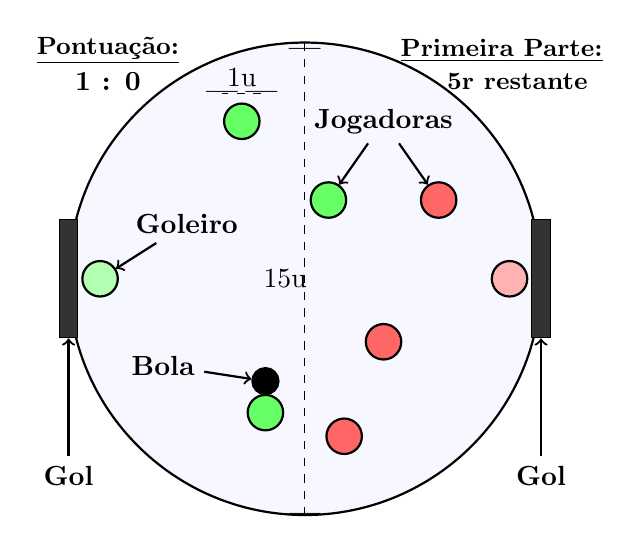
\begin{tikzpicture}[]
	\tikzstyle{test}=[thick, draw, circle, align=center]					
	\node[fill=blue!3!white, test, thick ,minimum size = 6cm](tarea)at (0,0) {};

	\node[fill=red!60!white, test,minimum size = 0.45cm](player2)at (1.7,1) {};
	\node[fill=red!60!white, test,minimum size = 0.45cm](target)at (1,-0.8) {};
	\node[fill=red!60!white, test,minimum size = 0.45cm](target)at (0.5,-2) {};

	\node[fill=green!60!white, test,minimum size = 0.45cm](target)at (-0.8,2) {};
	\node[](a1)at (-0.55,2.35) {\bf |};
	\node[](a2)at (-1.05,2.35) {\bf |};
	\node[](a2)at (-0.8,2.55) {1u};
	\draw[-, dashed](-0.55,2.35) -- (-1.05,2.35);
	
	\node[fill=green!60!white, test,minimum size = 0.45cm](player)at (0.3,1) {};
	\node[fill=green!60!white, test,minimum size = 0.45cm](target)at (-0.5,-1.7) {};
	\node[fill=black, test,minimum size = 0.1cm](ball)at (-0.5,-1.3) {};		
	\node[](tball)at (-1.8,-1.1) {\bf Bola};
	\node[](tplayer)at (1,2) {\bf Jogadoras};
	\draw[->, thick](tball) -- (ball);
	\draw[->, thick](tplayer) -- (player);
	\draw[->, thick](tplayer) -- (player2);
	
	\node[](tgk)at (-1.5,0.7) {\bf Goleiro};
	\node[](tgoal)at (-3,-2.5) {\bf Gol};
	\node[fill=black!80!white, draw, rectangle,minimum height=1.5cm, minimum width=0.05cm](goal)at (-3,0) {};
	\node[fill=green!30!white, test,minimum size = 0.45cm](gk)at (-2.6,0) {};
	\draw[->, thick](tgk) -- (gk);
	\draw[->, thick](tgoal) -- (goal);
	
	\node[](tgoal2)at (3,-2.5) {\bf Gol};
	\node[fill=black!80!white, draw, rectangle,minimum height=1.5cm](goal2)at (3,0) {};
	\node[fill=red!30!white, test,minimum size = 0.45cm](target)at (2.6,0) {};
	\draw[->, thick](tgoal2) -- (goal2);
	
	\node[](se2)at (0,2.9) {\bf ---};
	\node[](se2)at (0,-3) {\bf ---};
	\draw[-, dashed](0,3) -- node[] {}(0,-3);
	\node[](sca)at (-0.25,0) {15u};		
	
	\node[](sca)at (2.5,2.9) {\small\bf\underline{Primeira Parte:}};
	\node[](sca)at (2.5,2.5) {\small\bf\hspace*{0.4cm}5r restante};
	\node[](sca)at (-2.5,2.9) {\small\bf\underline{Pontuação:}};
	\node[](sca)at (-2.5,2.5) {\bf 1 : 0};
	\end{tikzpicture}
	}
\end{figure}
%
\vfill
%
As proficiências do jogador em diferentes aspectos do jogo são definidas pelos 4 atributos a seguir:\ofrow
\accf{Pontos de fôlego (PF):} Representa sua durabilidade durante o jogo.
	A maioria das ações custam uma quantidade de PF para se executar.
	Quando seus PF alcançam 0, você pode continuar jogando, mas não pode realizar ações que custam PF.
%
\ofrow
%
\accf{Ataque (ATQ):} Melhora suas chances de passar e chutar a bola.\ofrow
\accf{Defesa (DEF):} Melhora suas chances de roubar e interceptar a bola.\ofrow
\accf{Velocidade (VE):} Determina o quão rápido você pode nadar.
%
\newpage
%
%\ofquote{"When you got the ball, you gotta score!"\\}{Tidus}
%
%\ofpar
%\begin{center}  \includegraphics[width=\columnwidth]{./art/blitz/stadium.jpg} \end{center}
\includegraphics[width=\columnwidth]{./art/blitz/stadium.jpg}
%
\vfill
%
Durante cada turno, um jogador pode mergulhar uma distância total até sua VE+1 em unidades e realizar uma das seguintes ações.
A única exceção é o goleiro, que fica em frente ao gol o tempo todo e somente reage aos chutes dos inimigos.
O conjunto de ações que você pode realizar muda a depender de se você tem ou não a bola.
%
\ofrow
%
\accf{Passe:} Você passa a bola a outro jogador.
A bola pode viajar uma distância máxima igual a seu ATQ+1d em unidades.
Enquanto realizando o passe, cada oponente dentro de 1u de você pode tentar bloquear a bola.
Ao fazer isso, cada bloqueador reduz a distância do passe pela sua DEF+1d.
Se essa distância for reduzida a 0, ele pega a bola.
Se a bola passa de todos os bloqueadores, mas não alcança seu alvo, o jogador mais próximo a pega.
%	
\ofrow
%
\accf{Chute:} Você chuta a bola ao gol.
A bola pode viajar uma distância máxima igual a seu ATQ+1d em unidades.
Primeiro, cada chute pode ser bloqueado por oponentes próximos da mesma maneira que o passe. Assim, se a bola alcança o gol, o goleiro pode tentar pegá-la.
Se a DEF+1d do goleiro é maior do que a distância restante da bola, ele a pega, do contrário você pontua.
Se o goleiro pega a bola, ele pode imediatamente fazer um passe que não pode ser bloqueado. Se um ponto foi marcado, então um novo pontapé inicial será realizado ao inicio da próxima partida.
Cada chute custa a você uma quantidade de PF igual ao seu ATQ.
%	
\ofrow
%
\accf{Encontrão:} Você rouba a bola de um jogador que esteja a 1u.
Se sua DEF+1 é maior do que a DEF+1d do alvo, então você rouba a bola com sucesso. Também, adicione 1d à sua rolagem, para cada encontrão que o alvo receber desde seu último turno.
Ao realizar o encontrão, você também pode disparar a uma distância de sua VE+1 em unidades.
Cada encontrão custa uma quantidade de PF igual à sua DEF.
%
\ofrow
%	
\accf{Técnica:}
Técnicas são habilidades especiais que podem te ajudar a vencer um jogo.
Cada técnica contém seu efeito e custo em PF na sua descrição.
Uma lista de técnicas é mostrada na próxima página.
%
\vfill
%
Durante o jogo, os jogadores podem sofrer os seguintes efeitos por uma duração limitada.\ofrow
\accf{Veneno:} No início de cada turno, seu PF atual é reduzida em 10\% de seu máximo.\ofrow
\accf{Enfraquecido:} Seu ATQ, DEF e PF são reduzidos pela metade.\ofrow
\accf{Soneca:} Seus turnos são pulados e você não pode pegar ou bloquear a bola.
Quando um jogador passa para você enquanto estiver dormindo, você acorda e a bola é recebida pelo jogador mais próximo.
%
\clearpage
%
\ofquote{"Este é o chute Jecht, não é?"\\}{Yuna}\ofpar
%
\includegraphics[width=\columnwidth]{./art/blitz/ingame.jpg}
%
\ofpar
%
Todos os atributos de um jogador de Blitzball são derivados e melhorados pelos seus atributos de combate como a seguir:\ofrow
\accf{Pontos de fôlego = Pontos de vida + Pontos de mana} \ofrow
\accf{Ataque = Força + Magia} \ofrow
\accf{Defesa = Defesa (físca) + Resistência} \ofrow
\accf{Velocidade = Agilidade} \ofrow
%
Então se um personagem jogador aumenta de nível fora de uma partida e ganha FOR+1, seu ATQ também é aumentado em +1.
Para evitar confusão, os atributos de Blitzball devem ser acompanhados separadamente daqueles de combate.
No início cada jogador já sabe uma técnica a sua escolha.
Cada jogador aprende até 3 técnicas no máximo, ao observar outros jogadores que as executam.
Se durante uma partida, alguém a 3u de você executa uma técnica, você pode tentar passar num teste de DF~9 para aprendê-la.
Se já conhecer 3, você pode esquecer uma delas para substituir pela nova. Jogar Blitzball é uma fonte de experiência para os personagens jogadores, o que os ajudam a alcançar marcos na aventura mais rapidamente.
Além do mais, vencedores do Blitzball são normalmente premiados com várias recompensas e prêmios, incluindo equipamentos, itens e Gil.
%
\vfill
%
\oftable{p{0.15\columnwidth} l p{0.73\columnwidth}}
{\accf{Técnica} & \accf{PF} & \accf{Efeito}}
{
	Chute Jecht & 20 & Você dá um chute que não pode ser bloqueado, exceto pelo goleiro.\ofrow
	Luvas de agarrar & 8 & Até o inicio de seu próximo turno, adicione 1d a sua DEF enquanto tenta pegar um passe ou chute. \ofrow
	Parrudo & 8 & Até o fim de seu próximo turno, sua DEF aumenta em um valor igual a seu ATQ.\ofrow
	Espírito dos\newline auroques & 12 & Todos os aliados dentro de 5u aumentam seu ATQ e DEF em 3 até o início de seu próximo turno. \ofrow
	Passe\newline drenante & 8 & Você passa a bola, em que se adiciona 3u à distância dela. Cada jogador que falhar ao interceptar a bola, perde 5 PF e seu PF aumenta na mesma quantidade.\ofrow
}
%
\newpage
%
\oftable{p{0.16\columnwidth} l p{0.73\columnwidth}}
{\accf{Técnica} & \accf{PF} & \accf{Efeito}}
{
%	Jecht Shot & 20 & You make a shot, that cannot be blocked by any player except the goalkeeper.\ofrow
	Chute\newline esfera & 15 & Chute e adiciona 2d em unidades a distância da bola.\ofrow
	Chute\newline voleio & 6 & Ao receber um passe ou pegar a bola antes do início de seu próximo turno, você pode chutar imediatamente. \ofrow
	Chute\newline venenoso & 10 & Chute e adiciona 3u à distância da bola. Cada jogador que tentar bloqueá-la faz um teste de DF~8 ou fica envenenado por 3 rodadas.\ofrow
	Chute Enfraquecedor & 10 & Chute e adiciona 3u à distância da bola. Cada jogador que tentar bloqueá-la faz um teste de DF~8 ou fica Enfraquecido por 3 rodadas.\ofrow
	Chute\newline soneca & 10 & Chute e adiciona 3u à distância da bola. Cada jogador que tentar bloqueá-la faz um teste de DF~8 ou fica Dormindo por 3 rodadas.\ofrow
	Passe Enfraquecedor & 8 & Passe e adiciona 3u à distância da bola. Cada jogador que tentar bloqueá-la faz um teste de DF~8 ou fica Enfraquecido por 3 rodadas. \ofrow
	Passe\newline venenoso & 8 & Passe e adiciona 3u à distância da bola. Cada jogador que tentar bloqueá-la faz um teste de DF~8 ou fica Envenenado por 3 rodadas. \ofrow
	Passe\newline soneca & 8 & Passe e adiciona 3u à distância da bola. Cada jogador que tentar bloqueá-la faz um teste de DF~8 ou fica Dormindo por 3 rodadas.\ofrow
	Encontrão\newline venenoso & 10 & Dê um encontrão e adiciona +3 à sua DEF atual. Cada jogador que tentar bloqueá-la faz um teste de DF~8 ou fica Envenenado por 3 rodadas.\ofrow
	Encontrão\newline soneca & 10 & Dê um encontrão e adiciona +3 à sua DEF atual. Cada jogador que tentar bloqueá-la faze um teste de DF~8 ou fica Dormindo por 3 rodadas.\ofrow
	Encontrão Enfraquecedor & 10 & Dê um encontrão e adiciona +3 à sua DEF atual. Cada jogador que tentar bloqueá-la faz um teste de DF~8 ou fica Enfraquecido por 3 rodadas. \ofrow
	Encontrão\newline drenante & 10 & Dê um encontrão e adiciona +3 à sua DEF atual. Cada jogador que tentar bloqueá-la faz um teste de DF~8 ou seu PF é reduzido em -5 e o seu PF aumenta na mesma quantidade.\ofrow
	Encontrão\newline escorrega & 7 & Até o início do seu próximo turno, cada oponente que tentar dar um encontrão em você tem que fazer um teste de DF~8 primeiro ou errará o encontrão.\ofrow
	Defesa \newline de Elite & 8 & Até o início de seu próximo turno, quando um oponente se mover dentro de 1u de você, você pode dar um encontrão nele imediatamente.\ofrow
}
%
\clearpage
%
\end{document}